

\chapter{A statistical model for basal sliding}

Basal sliding is a source of great uncertainty in glacier dynamics.  Yet it is the primary control on the fast flow of ice, responsible for more than 90\% of the flux of ice into the Earth's oceans.  Mathematical models of basal sliding typically relate the speed of sliding to the shear stress as well as basal water pressure, topography, and composition.  To date, a general `sliding law' has eluded investigators at least in part due to a lack of observational data.  In recent years, Interferometric Synthetic Aperture Radar (InSAR) surface velocity observations have grown from a few outlet glaciers to nearly complete coverage of both Antarctica and Greenland.  Reported errors in these data sets are typically less than 1\% of the observed speed.  These data, in turn, can be inverted using a thermo-mechanically coupled higher-order ice sheet model.  The result of this inversion is a continuous basal friction field.  While the inverse process for determining basal friction, and hence basal sliding rates, is dependent on model assumptions regarding the mathematical formulation of ice dynamics, these inversion results nonetheless represent the scientific community's best estimate of basal sliding rates.  In this work, we will focus on basal friction fields determined through inverse modeling of the the observed surface speed.  We will treat these modeled basal friction fields as observations, effectively removing the primary obstacle of formulating a general sliding law.  Our approach utilizes dual general and generalized linear models, utilizing possibly transformed independent and dependent variables of the control model as explanatory variables, complete with all 2nd order interactions.  The resulting statistically generated basal friction fields produce a surface velocity similar to the observations, while the linear-model coefficients offer some physical insight into the corresponding variable's effect on basal sliding.

By applying the control method \citep{macayeal_1993} over Antarctica and Greenland, we generate high-resolution-basal-friction fields ($\beta$) which we then use to form the general linear model, 
$$\bm{\beta} = \mat{X} \bm{\alpha} + \bm{\epsilon},$$
where the design matrix $\mat{X}$ includes a subset of the independent and dependent variables of the control model, along with their interactions.  It is our hope that the statistically generated $\bm{\hat{\beta}}$-fields which result after solving for the parameters $\bm{\alpha}$ may be used to generate time-dependent-basal-friction values for an evolving ice-sheet.

\begin{figure}
  \centering
    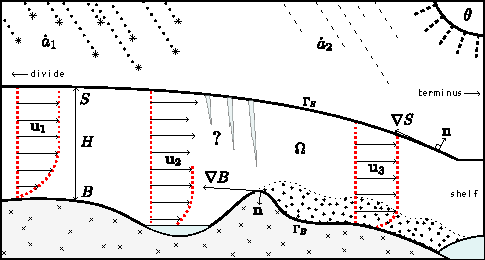
\includegraphics[width=\linewidth]{images/ice_profile.pdf}
	\caption[Basal sliding diagram]{Illustration of the complex mechanics of an ice-sheet with surface boundary $\Gamma_S$, basal boundary $\Gamma_B$, interior $\Omega$, and outward-pointing normal vector $\mathbf{n}$.  The velocity profiles (dashed red) depend heavily on basal traction; for example, the velocity profile $\mathbf{u}_1$ is frozen to the bed, corresponding to very high basal traction.  However, if the ice is supported by a layer of water (a lake for example), as is the case for velocity profile $\mathbf{u}_2$, basal traction is very close to zero, and hence the velocity at the bed is much higher.  This region is also affected by crevasses, a phenomenon not accounted for mathematically; likewise the profile $\mathbf{u}_3$ is flowing over a layer of deformable till and contains sediment within the ice.  These \emph{internal} effects are included implicitly by optimizing the basal traction to match the observed surface velocity.  As such, the basal traction estimates in our statistical model also implicitly include these effects.  Note that the accumulation rate $\dot{a}$, surface energy $\theta$, thickness $H$, surface $S$, bed $B$, and topography gradients $\nabla S$ and $\nabla B$ vary over the ice-sheet.  We incorporate these variables as explanatory terms in our general linear model.}
\end{figure}

\section{Multiple linear regression}

After inverting for $\beta$, we form the model
\begin{align*}
  \bm{\beta} = \mat{X} \bm{\alpha} + \bm{\epsilon},
\end{align*}
for vector of friction coefficients $\bm{\beta}$ of length $n$, defined over $\Gamma_B$, parameter vector $\bm{\alpha}$ of dimension $p$, $n \times p$ design matrix $\mat{X}$, and length-$n$ error vector $\bm{\epsilon}$.  The assumptions implicit to this model are independent observational errors with equal variance and normality of errors,
$$\bm{\beta}\ |\ \mat{X} \distras{iid} \mathcal{N}\left( \mat{X}\bm{\alpha}, \sigma^2 \mat{I}\right),\hspace{8mm} \bm{\epsilon} \distras{iid}\mathcal{N}\left(\bm{0},\sigma^2\mat{I}\right)$$ 
which implies that the expected value $\Ex\left(\bm{\beta}|\bm{\alpha}, \mat{X}\right)$ is linear in $\mat{X}$.

In order satisfy the normality requirements we use the left-hand-side transformation $\ln\left(\bm{\beta}\right)$.  We also reduce the non-linearity of the expected value by appending all 2\sups{nd}-order interactions between variables to the design matrix $\mat{X}$ such that
\footnotesize
\begin{align*}
  \mat{X} = \begin{bmatrix}
        \mathbf{1} & \mathbf{x}_0 & \mathbf{x}_1 & \cdots & \mathbf{x}_p & \mathbf{x}_0 \star \mathbf{x}_1 & \mathbf{x}_0 \star \mathbf{x}_2 & \cdots & \mathbf{x}_0 \star \mathbf{x}_p & \cdots 
      \end{bmatrix},
\end{align*}
\normalsize
where $\star$ indicates component-wise multiplication and $p$ is the number of original parameters, given in Table 2.

\begin{figure}
  \centering
    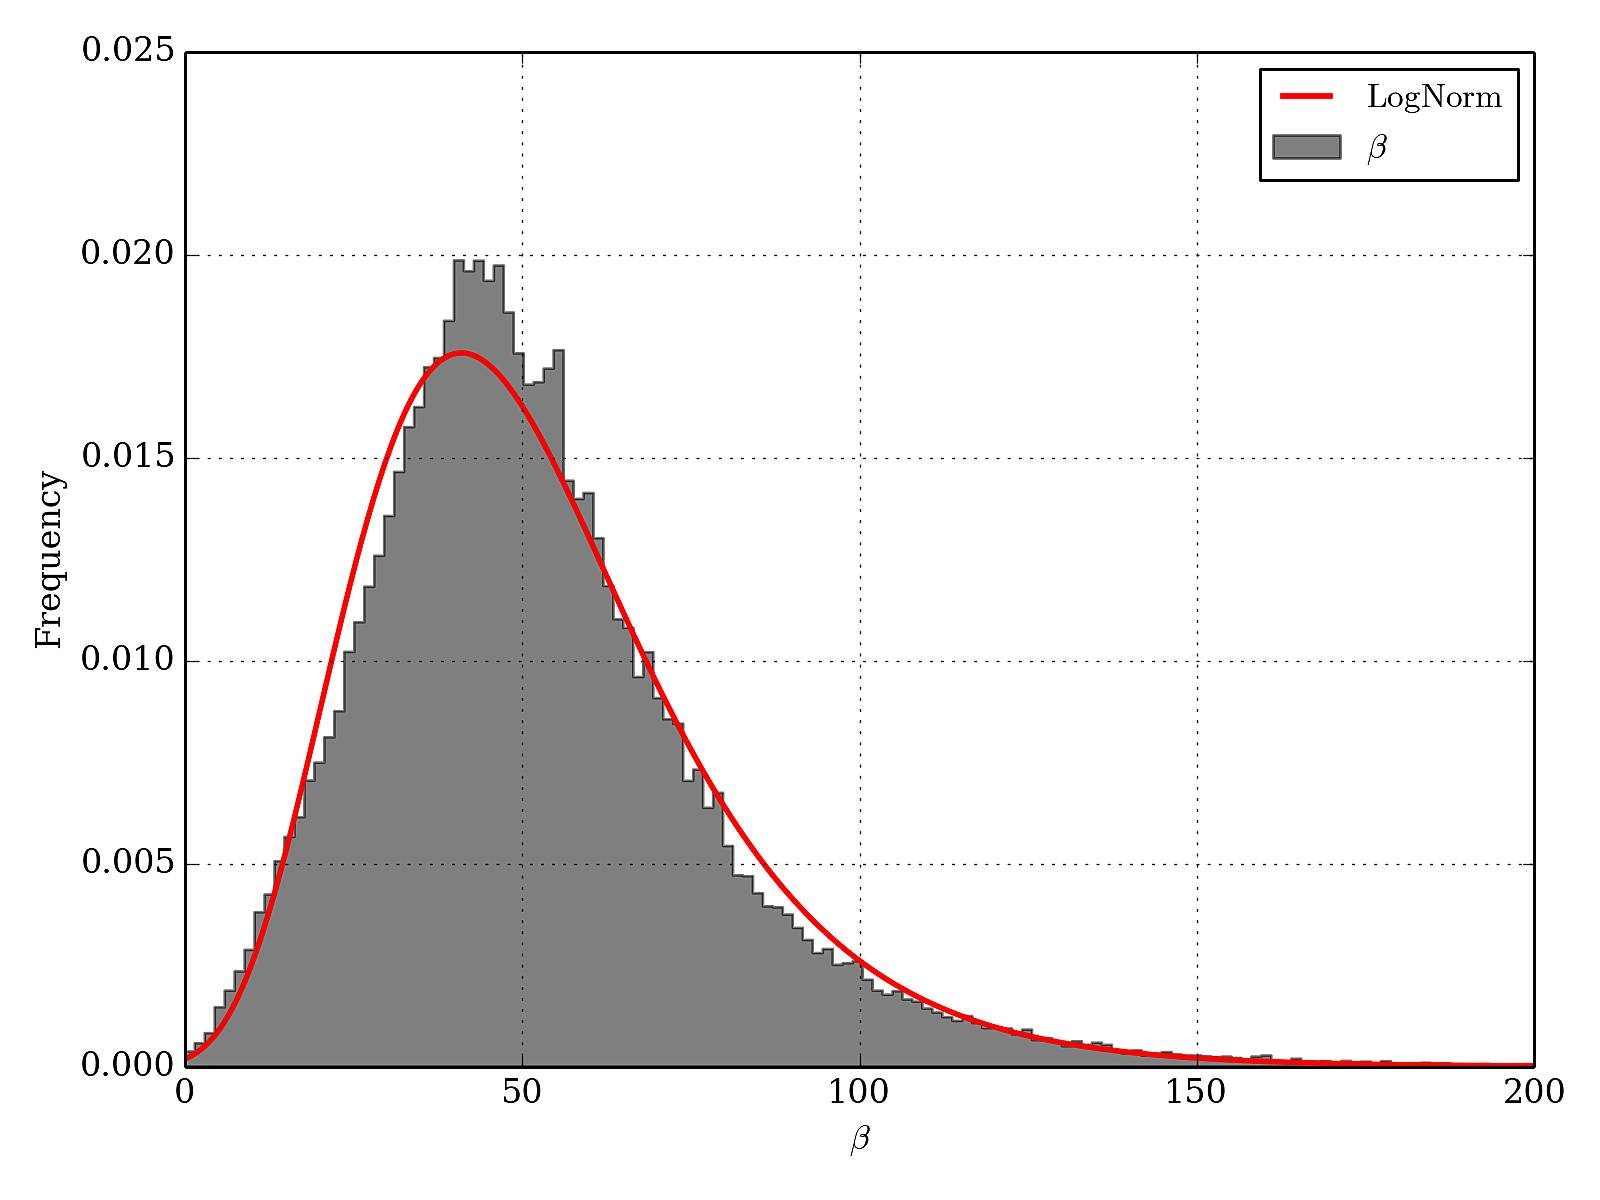
\includegraphics[width=\linewidth]{images/greenland/stats/beta_distribution.jpg}
  \caption[Basal traction distribution]{Distribution of assimilated $\beta$ field with log-normal distribution best-fit line.}
\end{figure}

\begin{table*}[t]
\centering
\footnotesize
  \caption[Basal sliding statistical model variables]{The variables used in the columns of the design matrix.}
\begin{tabular}{l|l|l|l}
  \textbf{Field} & \specialcell{\textbf{Variable and}\\\textbf{transformation}} & \textbf{Antarctica source} & \textbf{Greenland source} \\
  \hline
  surface height                     & $S$                                                & \citep{fretwell_2013} & \citep{bamber_2013}               \\
  surface temperature                & $T_S$                                              & \citep{lebrocq_2010}  & \citep{fausto_2009}               \\
  under sea-level ?                  & $D$                                                & \citep{fretwell_2013} & \citep{bamber_2013}               \\
  ice thickness                      & $H = S - B$                                        & \citep{fretwell_2013} & \citep{bamber_2013}               \\
  accumulation                       & $\dot{a}$                                          & \citep{lebrocq_2010}  & \citep{burgess_2010,annoortvanvanderveen_2001} \\
  modeled basal temperature          & $T_B$                                              & -                 & -                             \\
  modeled basal melt rate            & $M_B$                                              & -                 & -                             \\
  balance velocity                   & $\ln\left(\Vert \bar{\mathbf{u}} \Vert \right)$    & -                 & -                             \\
  modeled basal velocity norm        & $\ln\left(\Vert \mathbf{u}_B \Vert \right)$        & -                 & -                             \\
  surface slope in direction of flow & $\nabla_{\mathbf{u}} S$                            & -                 & -                             \\
  bed slope in direction of flow     & $\nabla_{\mathbf{u}} B$                            & -                 & -                             \\
  along flow driving stress          & $\tau_{id}$                                        & -                 & -                             \\
  across flow driving stress         & $\tau_{jd}$                                        & -                 & -                             \\
  long.\ stress along flow           & $\tau_{ii}$                                        & -                 & -                             \\
  lat.\ shear along flow             & $\tau_{ij}$                                        & -                 & -                             \\
  long.\ stress across flow          & $\tau_{ji}$                                        & -                 & -                             \\
  lat.\ shear across flow            & $\tau_{jj}$                                        & -                 & -                             \\
\end{tabular}
\end{table*}

\section{Generalized linear model}

The exponential-family form of the probability density function $f$ is defined as \citep{mccullagh_1989}
\begin{align*}
  f(y; \theta, \phi) = \exp\left\{ \frac{y\theta - b(\theta)}{a(\phi)} + c(y,\phi) \right\},
\end{align*}
with canonical parameter $\theta$, observation $y$, cumulant function $b(\theta)$, dispersion parameter $\phi$, and normalization function $c(y,\phi)$.

The normal density for our model with $y = \beta$ and $\Ex(\beta) = \mu$ is
\begin{align*}
  f(\beta; \mu, \sigma^2) &= \frac{1}{\sqrt{2\pi \sigma^2}} \exp\left\{ - \frac{(\beta - \mu)^2}{2\sigma^2} \right\} \\
  &= \exp\left\{ - \frac{(\beta - \mu)^2}{2\sigma^2} + \ln\left( \frac{1}{\sqrt{2\pi \sigma^2}} \right)  \right\} \\
  &= \exp\left\{ - \frac{(\beta - \mu)^2}{2\sigma^2} + \ln(1) - \ln\left( \sqrt{2\pi \sigma^2} \right)  \right\} \\
  &= \exp\left\{ - \frac{\beta^2 - 2\beta \mu + \mu^2}{2\sigma^2} - \frac{1}{2}\ln\left( 2\pi \sigma^2 \right)  \right\} \\
  &= \exp\left\{ \frac{\beta \mu - \mu^2 / 2}{\sigma^2} - \frac{\beta^2}{2\sigma^2} - \frac{1}{2}\ln\left( 2\pi \sigma^2 \right)  \right\}.
\end{align*}
Thus we have determined the exponential-family form with 
\begin{align*}
  \theta = \mu, \hspace{5mm} \phi = \sigma^2, \hspace{5mm} b(\mu) = \frac{\mu^2}{2}, \hspace{5mm} a(\sigma^2) = \sigma^2,
\end{align*}
and
\begin{align*}
  c(\beta,\sigma^2) &= -\left( \frac{\beta^2}{2\sigma^2} + \frac{1}{2}\ln\left( 2\pi \sigma^2 \right) \right).
\end{align*}

Using i.i.d.\ observations $\bm{\beta}$, the joint density may be stated
$$\bm{f}(\bm{\beta}; \bm{\mu}, \sigma^2) = \prod_{i=1}^n \exp\left\{ \frac{\beta_i \mu_i - \mu_i^2 / 2}{\sigma^2} - \frac{\beta_i^2}{2\sigma^2} - \frac{1}{2}\ln\left( 2\pi \sigma^2 \right)  \right\}.$$

If we assume a log-normal model \citep{hardin_2012}, we relate the expected value of the observations to the linear predictor through the \emph{link function} $g\left(\cdot\right) = \ln\left(\cdot\right)$.  Hence the new predictor variable is
\begin{align*}
  \eta_i &= g\left(\mu_i\right) = \ln\left(\mu_i\right) = \mat{X}_i \bm{\alpha},
\end{align*}
where the mean may be recovered from the inverse link function
\begin{align*}
  \mu_i &= g^{-1}\left(\eta_i\right) = \exp\left(\eta_i\right) = \exp\left( \mat{X}_i \bm{\alpha} \right).
\end{align*}

Therefore, the log-normal probability density as a function of $\eta$ is,
\begin{align*}
  f(\beta; \eta, \sigma^2) &= \exp\left\{ \frac{\beta \exp\left(\eta \right) - \left( \exp\left(\eta \right) \right)^2 / 2}{\sigma^2} - \frac{\beta^2}{2\sigma^2} - \frac{1}{2}\ln\left( 2\pi \sigma^2 \right)  \right\},
\end{align*}
with
$$\theta = \exp\left( \eta \right), \hspace{5mm} \phi = \sigma^2, \hspace{5mm} b(\eta) = \frac{\left( \exp\left( \eta \right) \right)^2}{2}, \hspace{5mm} a(\sigma^2) = \sigma^2,$$
and
$$c(\beta,\sigma^2) = - \left( \frac{\beta^2}{2\sigma^2} + \frac{1}{2}\ln\left( 2\pi \sigma^2 \right) \right).$$

\section{Maximum likelihood}

Expressing the distribution in exponential-family form allows us to easily state the log-likelihood function $\bm{\ell} = \ln(\bm{f})$,
\begin{align*}
  \bm{\ell}(\bm{\mu}, \sigma^2; \bm{\beta}) = \sum_{i=1}^n \left\{ \frac{\beta_i \mu_i - b(\mu_i)}{a(\sigma^2)} + c(\beta_i,\sigma^2) \right\}.
\end{align*}

%===============================================================================
%
%It can be shown by differentiating with respect to $\mu_i$ the identity
%$$\int f(\beta_i; \mu_i, \sigma^2) \d{\beta_i} \equiv 1$$
%that
%\begin{align*}
%  \Ex\left( \parder{\ell_i}{\mu_i} \right) = 0 \hspace{5mm} \text{and} \hspace{5mm}
%  \Ex\left( \parder[2]{\ell_i}{\mu_i} \right) + \Ex\left( \parder{\ell_i}{\mu_i} \right)^2 = 0,
%\end{align*}
%such that with
%\begin{align*}
%  \parder{\ell_i}{\mu_i} = \frac{\beta_i - b'(\mu_i)}{a(\sigma^2)}, \hspace{10mm} 
%  \parder[2]{\ell_i}{\mu_i} = -\frac{b''(\mu_i)}{a(\sigma^2)}
%\end{align*}
%we have
%\begin{align*}
%  0 &= \Ex\left( \parder{\ell_i}{\mu_i} \right) &&= \frac{\Ex\left(\beta_i\right) - b'(\mu_i)}{a(\sigma^2)} \implies \Ex\left( \beta_i \right) = b'(\mu_i) = \mu_i, \\
%  0 &= \Ex\left( \parder[2]{\ell_i}{\mu_i} \right) + \Ex\left( \parder{\ell_i}{\mu_i} \right)^2 &&= -\frac{b''(\mu_i)}{a(\sigma^2)} + \frac{\Ex\left[\left(\beta_i - \mu_i \right)^2\right]}{\left(a(\sigma^2)\right)^2} \\
%  & &&= \frac{-b''(\mu_i) a(\sigma^2) + \var\left(\beta_i\right)}{\left(a(\sigma^2)\right)^2}.
%\end{align*}
%Therefore,
%$$\Ex\left( \beta_i \right) = \mu_i = b'(\mu_i), \hspace{8mm} \var\left(\beta_i\right) = V(\mu_i) a(\sigma^2),$$
%with variance function $V(\mu_i) = b''(\mu_i)$ and $a(\sigma^2) = \sigma^2 / w_i$ with prior weight $w_i$.
%
%===============================================================================

It can be shown by differentiating with respect to $\mu$ the identity
$$\int f(\beta; \mu, \sigma^2) \d{\beta} \equiv 1$$
that
\begin{align*}
  \Ex\left( \parder{\ell}{\mu} \right) = 0 \hspace{5mm} \text{and} \hspace{5mm}
  \Ex\left( \parder[2]{\ell}{\mu} \right) + \Ex\left( \parder{\ell}{\mu} \right)^2 = 0,
\end{align*}
such that with
\begin{align*}
  \parder{\ell}{\mu} = \frac{\beta - b'(\mu)}{a(\sigma^2)}, \hspace{10mm} 
  \parder[2]{\ell}{\mu} = -\frac{b''(\mu)}{a(\sigma^2)}
\end{align*}
we have
\begin{align*}
  0 &= \Ex\left( \parder{\ell}{\mu} \right) &&= \frac{\Ex\left(\beta\right) - b'(\mu)}{a(\sigma^2)} \implies \Ex\left( \beta \right) = b'(\mu) = \mu, \\
  0 &= \Ex\left( \parder[2]{\ell}{\mu} \right) + \Ex\left( \parder{\ell}{\mu} \right)^2 &&= -\frac{b''(\mu)}{a(\sigma^2)} + \frac{\Ex\left[\left(\beta - \mu \right)^2\right]}{\left(a(\sigma^2)\right)^2} \\
  & &&= \frac{-b''(\mu) a(\sigma^2) + \var\left(\beta\right)}{\left(a(\sigma^2)\right)^2}.
\end{align*}
Therefore,
$$\Ex\left( \beta \right) = \mu = b'(\mu), \hspace{8mm} \var\left(\beta\right) = V(\mu) a(\sigma^2),$$
with variance function $V(\mu) = b''(\mu)$ and $a(\sigma^2) = \sigma^2 / w$ with prior weight $w$.

The maximum likelihood estimation of the parameters $\alpha_r$, $r \in 1,2,\ldots, p$ requires that
$$\sum_{i=1}^n \parder{\ell_i}{\alpha_r} = 0,$$
where we apply the chain rule
\begin{align*}
  \parder{\ell_i}{\alpha_r} &= \parder{\ell_i}{\mu_i} \parder{\mu_i}{\eta_i} \parder{\eta_i}{\alpha_r},
\end{align*}
and derive
\begin{align*}
  \parder{\ell_i}{\mu_i} &=  \frac{\beta_i - b'(\theta_i)}{a(\sigma^2)} = \frac{\left(\beta_i - \mu_i\right)w_i}{\sigma^2} \\
  \parder{\eta_i}{\alpha_r} &= \parder{}{\alpha_r} X_{ir} \alpha_r = X_{ir}.
\end{align*}
Therefore,
\begin{align*}
  \parder{\ell_i}{\alpha_r} &= \left( \frac{\left(\beta_i - \mu_i\right)w_i}{\sigma^2} \right) \left( \parder{\mu_i}{\eta_i} \right) X_{ir} \\
  &= \frac{w_i}{\sigma^2} \left( \parder{\mu_i}{\eta_i} \right)^2 \left(\beta_i - \mu_i\right) \left( \parder{\eta_i}{\mu_i} \right) X_{ir}.
\end{align*}

\section{Deriving optimal parameters}

The estimated parameters $\bm{\hat{\alpha}}$ may be determined by using Newton's method using the first two terms of the Taylor series of the derivative of $\bm{\ell}$ expanded about $\bm{\alpha}_0$,
\begin{align*}
  \mathbf{0} &= \parder{\bm{\ell}}{\bm{\alpha}} \\
  &\approx \left( \parder{\bm{\ell}}{\bm{\alpha}} \right)_0 + \left( \frac{\partial^2 \bm{\ell}}{\partial \bm{\alpha} \partial \bm{\alpha}\T} \right)_0 \left( \bm{\alpha} - \bm{\alpha}_0 \right) \\
  \implies \bm{\alpha} &\approx \bm{\alpha}_0 - \left( \frac{\partial^2 \bm{\ell}}{\partial \bm{\alpha} \partial \bm{\alpha}\T} \right)_0^{-1} \left( \parder{\bm{\ell}}{\bm{\alpha}} \right)_0,
\end{align*}
where the derivatives are evaluated at $\bm{\alpha}_0$.  Using the method of Fisher scoring, we approximate the $p \times p$ Hessian matrix from its expectation.  For a single observation $i$, the $(r,k)$ element may be thus derived,
\begin{align*}
  \frac{\partial^2 \ell_i}{\partial \alpha_r \partial \alpha_k} &\approx - \Ex\left[ \frac{\partial^2 \ell_i}{\partial \alpha_r \partial \alpha_k} \right] \\
  &= - \Ex\left[ \parder{\ell_i}{\alpha_r} \parder{\ell_i}{\alpha_k} \right] \\
  &= - \Ex\left[ \left( \frac{w_i}{\sigma^2} \right)^2 \left( \parder{\mu_i}{\eta_i} \right)^4 \left(\beta_i - \mu_i\right)^2 \left( \parder{\eta_i}{\mu_i} \right)^2 X_{ir} X_{ik} \right] \\
  &= - \left( \frac{w_i}{\sigma^2} \right)^2 \left( \parder{\mu_i}{\eta_i} \right)^2 \Ex\left[ \left(\beta_i - \mu_i\right)^2 \right] X_{ir} X_{ik} \\
  &= - \left( \frac{w_i}{\sigma^2} \right)^2 \left( \parder{\mu_i}{\eta_i} \right)^2 \var\left(\beta_i\right) X_{ir} X_{ik} \\
  &= - \left( \frac{w_i}{\sigma^2} \right)^2 \left( \parder{\mu_i}{\eta_i} \right)^2 \frac{\sigma^2}{w_i} X_{ir} X_{ik} \\
  &= - \frac{w_i}{\sigma^2} \left( \parder{\mu_i}{\eta_i} \right)^2 X_{ir} X_{ik}.
\end{align*}
The matrix-vector form for the first derivative can be derived,
\begin{align*}
  \parder{\ell}{\alpha_r} &= \sum_{i=1}^n \parder{\ell_i}{\alpha_r} = \sum_{i=1}^n \frac{w_i}{\sigma^2} \left( \parder{\mu_i}{\eta_i} \right)^2 \left(\beta_i - \mu_i\right) \left( \parder{\eta_i}{\mu_i} \right) X_{ir} \\
  &= \Bigg[ \mat{X}_{:,r} \Bigg]_{1 \times n}\T \cdot \Bigg[ \frac{\mathbf{w}}{\sigma^2} \left( \parder{\bm{\mu}}{\bm{\eta}} \right)^2 \big(\bm{\beta} - \bm{\mu}\big) \left( \parder{\bm{\eta}}{\bm{\mu}} \right) \Bigg]_{n \times 1} \\
  \implies \left( \parder{\bm{\ell}}{\bm{\alpha}} \right)_0 &= \mat{X}\T \mat{W}_0 \big(\bm{\beta} - \bm{\mu}_0\big) \left( \parder{\bm{\eta}}{\bm{\mu}} \right)_0,
\end{align*}
where $\mat{W}_0$ is the $n \times n$ diagonal matrix evaluated at iterate 0,
\begin{align*}
  \mat{W}_0 = \diag\left\{ \frac{\mathbf{w}}{\sigma^2} \left( \parder{\bm{\mu}}{\bm{\eta}} \right)_0^2 \right\}.
\end{align*}
The matrix form for the second derivative is
\begin{align*}
  \frac{\partial^2 \ell}{\partial \alpha_r \partial \alpha_k} &= \sum_{i=1}^n \frac{\partial^2 \ell_i}{\partial \alpha_r \partial \alpha_k} = - \sum_{i=1}^n \frac{w_i}{\sigma^2} \left( \parder{\mu_i}{\eta_i} \right)^2 X_{ir} X_{ik} \\
  &= - \Bigg[ \mat{X}_{:,r} \Bigg]_{1 \times n}\T \cdot \Bigg[ \mat{W} \Bigg]_{n \times n} \cdot \Bigg[ \mat{X}_{:,k} \Bigg]_{n \times 1} \\
  \implies \left( \frac{\partial^2 \bm{\ell}}{\partial \bm{\alpha} \partial \bm{\alpha}\T} \right)_0 &= - \mat{X}\T \mat{W}_0 \mat{X}.
\end{align*}

Therefore, we have the matrix-vector form of the estimation,
\begin{align*}
  \mathbf{0} &= \left( \parder{\bm{\ell}}{\bm{\alpha}} \right)_0 + \left( \frac{\partial^2 \bm{\ell}}{\partial \bm{\alpha} \partial \bm{\alpha}\T} \right)_0 \left( \bm{\alpha} - \bm{\alpha}_0 \right) \\
  &= \mat{X}\T \mat{W}_0 \big(\bm{\beta} - \bm{\mu}_0\big) \left( \parder{\bm{\eta}}{\bm{\mu}} \right)_0 - \mat{X}\T \mat{W}_0 \mat{X} \left( \bm{\alpha} - \bm{\alpha}_0 \right).
\end{align*}
In order to include the predictor variable for observation $i$,
\begin{align*}
  \eta_i &= \sum_{k=1}^p X_{ik} \alpha_k,
\end{align*}
in the estimation, we multiply the residual of this equation by the common factor
\begin{align*}
  \frac{w_i}{\sigma^2} \left( \parder{\mu_i}{\eta_i} \right)^2 X_{ir},
\end{align*}
providing the relation
\begin{align*}
  0 &= \frac{w_i}{\sigma^2} \left( \parder{\mu_i}{\eta_i} \right)^2 X_{ir} \eta_i - \frac{w_i}{\sigma^2} \left( \parder{\mu_i}{\eta_i} \right)^2 X_{ir} \sum_{k=1}^p X_{ik} \alpha_k \\
  &= \frac{w_i}{\sigma^2} \left( \parder{\mu_i}{\eta_i} \right)^2 X_{ir} \eta_i - \sum_{k=1}^p \frac{w_i}{\sigma^2} \left( \parder{\mu_i}{\eta_i} \right)^2 X_{ir} X_{ik} \alpha_k,
\end{align*}
which when summed over all $i$ gives
\begin{align*}
  0 = &\sum_{i=1}^n \frac{w_i}{\sigma^2} \left( \parder{\mu_i}{\eta_i} \right)^2 X_{ir} \eta_i - \sum_{i=1}^n \sum_{k=1}^p \frac{w_i}{\sigma^2} \left( \parder{\mu_i}{\eta_i} \right)^2 X_{ir} X_{ik} \alpha_k \\
  = &+ \Bigg[ \mat{X}_{:,r} \Bigg]_{1 \times n}\T \cdot \Bigg[ \frac{\mathbf{w}}{\sigma^2} \left( \parder{\bm{\mu}}{\bm{\eta}} \right)^2 \bm{\eta} \Bigg]_{n \times 1} \\
    &- \sum_{k=1}^p \Bigg[ \mat{X}_{:,r} \Bigg]_{1 \times n}\T \cdot \Bigg[ \mat{W} \Bigg]_{n \times n} \cdot \Bigg[ \mat{X}_{:,k} \Bigg]_{n \times 1} \alpha_k \\
  \implies \mathbf{0} = &\mat{X}\T \mat{W}_0 \bm{\eta}_0 - \mat{X}\T \mat{W}_0 \mat{X} \bm{\alpha}_0.
\end{align*}
We now add this to equation [?],
\begin{align*}
  \mathbf{0} = &+ \mat{X}\T \mat{W}_0 \big(\bm{\beta} - \bm{\mu}_0 \big) \left( \parder{\bm{\eta}}{\bm{\mu}} \right)_0 - \mat{X}\T \mat{W}_0 \mat{X} \left( \bm{\alpha} - \bm{\alpha}_0 \right) \\
  &+ \mat{X}\T \mat{W}_0 \bm{\eta}_0 - \mat{X}\T \mat{W}_0 \mat{X} \bm{\alpha}_0 \\
  = &+ \mat{X}\T \mat{W}_0 \Bigg[ \bm{\eta}_0 + \big(\bm{\beta} - \bm{\mu}_0 \big) \left( \parder{\bm{\eta}}{\bm{\mu}} \right)_0 \Bigg] - \mat{X}\T \mat{W}_0 \mat{X} \left( \bm{\alpha} - \bm{\alpha}_0 + \bm{\alpha}_0 \right) \\
  = &+ \mat{X}\T \mat{W}_0 \Bigg[ \bm{\eta}_0 + \big(\bm{\beta} - \bm{\mu}_0 \big) \left( \parder{\bm{\eta}}{\bm{\mu}} \right)_0 \Bigg] - \mat{X}\T \mat{W}_0 \mat{X} \bm{\alpha}.
\end{align*}
We then define the new adjusted dependent variable
$$\mathbf{z} = \bm{\eta}_0 + \big(\bm{\beta} - \bm{\mu}_0\big) \left( \parder{\bm{\eta}}{\bm{\mu}} \right)_0$$
and set $\bm{\alpha} = \bm{\hat{\alpha}}$ and $\bm{\eta}_0 = \bm{\hat{\eta}}_0$ so that we can solve for the estimated parameters
\begin{align*}
  \mathbf{0} &= \mat{X}\T \mat{W}_0 \mathbf{z} - \mat{X}\T \mat{W}_0 \mat{X} \bm{\hat{\alpha}} \\
  \implies \hat{\bm{\alpha}} &= \left( \mat{X}\T \mat{W}_0 \mat{X} \right)^{-1} \mat{X}\T \mat{W}_0 \mathbf{z}.
\end{align*}
Note that for our log-normal model, we use the substitutions
\begin{align*}
  \bm{\hat{\mu}}_0 = \exp\left( \bm{\hat{\eta}}_0 \right), \hspace{5mm} \left( \parder{\bm{\hat{\eta}}}{\bm{\hat{\mu}}} \right)_0 = \frac{1}{\bm{\hat{\mu}}_0},
\end{align*}
such that
\begin{align*}
  \mathbf{z} = \bm{\hat{\eta}}_0 + \frac{\bm{\beta}}{\bm{\hat{\mu}}_0} - \mathbf{1}, \hspace{10mm} 
  \mat{W}_0 = \diag\left\{ \frac{\mathbf{w} \bm{\hat{\mu}}_0^2}{\sigma^2} \right\}.
\end{align*}

This model also allows us to easily estimate the variance of the parameters $\hat{\alpha}$, taken to be the diagonal of the expected Hessian matrix \citep{hardin_2012}, \ie,
\begin{align*}
 \var\left( \bm{\hat{\alpha}} \right) &= \diag\left\{ \left( \mat{X}\T \mat{W} \mat{X} \right)^{-1} \right\};
\end{align*}
the estimate of the error variance $\hat{\sigma}^2$ from the mean standard error,
$$\hat{\sigma}^2 = \frac{1}{n - p} \sum_{i=1}^n \left( \beta_i - \hat{\beta}_i \right)^2;$$
and the estimated standard error of the parameters,
\begin{align*}
 \mathrm{SE}\left( \bm{\hat{\alpha}} \right) &= \sqrt{ \diag\left\{ \left( \mat{X}\T \mat{W} \mat{X} \right)^{-1} \right\} }.
\end{align*}
With the standard errors in hand, we then calculate the Bonferroni-corrected 95\% confidence intervals via
\begin{align*}
  \mathrm{CI}_{\pm} \left( \bm{\hat{\alpha}} \right) = \bm{\hat{\alpha}} \pm t_{.95}^{\mathrm{bonf}} \cdot \mathrm{SE}\left( \bm{\hat{\alpha}} \right),
\end{align*}
where $t_{.95}^{\mathrm{bonf}}$ is derived from Student's t-distribution with parameter $n-p$ evaluated at $1 - 0.05/p$.  Using the Bonferroni correction takes into account the fact that we are testing $p$ hypotheses, one for each coefficient, and as such the confidence intervals need to be increased due to the added uncertainty.

\section{Analytic Hessian?}

The Hessian matrix might be evaluated analytically,
\begin{align*}
  \frac{\partial^2 \ell_i}{\partial \alpha_r \partial \alpha_k} &= \parder{}{\alpha_k} \left[ \left( \frac{(\beta_i - \mu_i)w_i}{\sigma^2} \right) \mu_i X_{ir} \right] \\
  &= \parder{}{\alpha_k} \Big[ \left( \beta_i - \mu_i \right) \mu_i \Big] \frac{w_i X_{ir}}{\sigma^2} \\
  &= \left[ \mu_i \parder{}{\alpha_k} \left( \beta_i - \mu_i \right) + \parder{\mu_i}{\alpha_k} \left( \beta_i - \mu_i \right) \right] \frac{w_i X_{ir}}{\sigma^2} \\
  &= \left[ - \mu_i \parder{\mu_i}{\alpha_k} + \parder{\mu_i}{\alpha_k} \left( \beta_i - \mu_i \right) \right] \frac{w_i X_{ir}}{\sigma^2} \\
  &= \parder{\mu_i}{\alpha_k} \Big[ \left( \beta_i - \mu_i \right) - \mu_i \Big] \frac{w_i X_{ir}}{\sigma^2},
\end{align*}
which if we use $\mu_i = \exp\left( \eta_i \right) = \exp\left( X_i \alpha \right)$,
\begin{align*}
  \parder{\mu_i}{\alpha_k} &= \parder{\mu_i}{\eta_i} \parder{\eta_i}{\alpha_k} \\
  &= \mu_i X_{ik},
\end{align*}
and we have
\begin{align*}
  \frac{\partial^2 \ell_i}{\partial \alpha_r \partial \alpha_k} &= \mu_i X_{ik} \left( \beta_i - 2\mu_i \right) \frac{w_i X_{ir}}{\sigma^2}.
\end{align*}
Therefore, the $(r,k)$ element of the symmetric Hessian matrix is
\begin{align*}
  \frac{\partial^2 \ell}{\partial \alpha_r \partial \alpha_k} &= \frac{1}{\sigma^2}\sum_{i=1}^n \left[ \mu_i \left( \beta_i - 2\mu_i \right) w_i X_{ir} X_{ik} \right],
\end{align*}
or in matrix-vector notation
\begin{align*}
  \frac{\partial^2 \ell}{\partial \alpha \partial \alpha\T} &= X\T W X,
\end{align*}
where
$$W = \diag\left\{ \frac{\mu \left( \beta - 2\mu \right) w}{\sigma^2} \right\} $$

The starting values for $\hat{\alpha}$ may be determined by assuming a constant-only model, \ie $\eta = \alpha_0$ and thus $\mu = \exp(\alpha_0)$.  The log-likelihood function becomes
\begin{align*}
  \parder{\ell}{\alpha_0} &= \sum_{i=1}^n \left[ \left( \frac{(\beta_i - \exp(\alpha_0))w_i}{\sigma^2} \right) \exp(\alpha_0) X_{i0} \right],
\end{align*}
and we solve using $X_{0} = \mathbf{1}$ and $w = \mathbf{1}$
\begin{align*}
  0 &= \sum_{i=1}^n \left[ \left( \frac{\beta_i - \exp\left( \hat{\alpha}_0 \right)}{\sigma^2} \right) \exp\left( \hat{\alpha}_0 \right) \right] \\
    &= \sum_{i=1}^n \left( \beta_i - \exp\left( \hat{\alpha}_0 \right) \right) \\
    &= \bar{\beta} - n \exp\left( \hat{\alpha}_0 \right).
\end{align*}
Our starting parameters are therefore $\hat{\alpha} = [ \hat{\alpha}_0\ 0\ \ldots\ 0]\T$ with
\begin{align*}
  \hat{\alpha}_0 &= \ln\left( \bar{\beta} \right) - \ln(n).
\end{align*}

\section{Prior weights}

A natural choice for prior weight $w_i$ for a structured grid of finite elements, is the ratio of cell area $h_i$ of element $i = 1,2,\ldots, n$ to total area of the basal surface $A$,
$$w_i = \frac{n h_i}{A}, \hspace{10mm} A = \sum_{i=1}^n h_i,$$
where $\mathbf{w}$ has the property that
$$\frac{1}{n}\sum_{i=1}^n w_i = 1.$$

Including this weight in the model eliminates the effect of cell size on the predictor $\bm{\hat{\eta}}$ and associated parameter estimates $\bm{\hat{\alpha}}$.

\section{Iterative procedure}

The same procedure used to minimize the residual of the nonlinear momentum equations, Newton-Raphson, may again be used to maximize the likelihood of the estimated parameters $\hat{\alpha}$ \citep{mccullagh_1989}.

To start the procedure, we use the model data itself as an initial guess, whereby
$$\bm{\hat{\mu}} = \left(\bm{\beta} + \mean(\bm{\beta}) \right) / 2, \hspace{8mm} \bm{\hat{\eta}} = \ln\left( \bm{\beta} \right).$$
This algorithm is outlined in Algorithm \ref{irls}.

\begin{algorithm}
  \normalsize
  \begin{algorithmic} 
    \State \textbf{INPUTS}: 
    \State \ \ \ $\phantom{r_{tol}}\mathllap{\bm{\beta}}$ - Observed friction vector.
    \State \ \ \ $\phantom{r_{tol}}\mathllap{\mat{X}}$ - Design matrix.
    \State \ \ \ $\phantom{r_{tol}}\mathllap{\mathbf{w}}$ - Prior weight vector.
    \State \ \ \ $r_{tol}$ - Relative tolerance to stop iterating.
    \State \textbf{OUTPUT}: 
    \State \ \ \ $\phantom{r_{tol}}\mathllap{\bm{\hat{\mu}}}$ - Estimated friction vector.
    \State \ \ \ $\phantom{r_{tol}}\mathllap{\bm{\hat{\alpha}}}$ - Parameter vector.
    \State \ \ \ $\phantom{r_{tol}}\mathllap{\mathbf{d}}$ - Discrepancy vector.
    \\
    \hrulefill
    \Function{GLM}{$\bm{\beta},\ \mat{X},\ \mathbf{w},\ r_{tol}$}
      \State $\phantom{\hat{\sigma}^2}\mathllap{\bm{\hat{\mu}}} := \left(\bm{\beta} + \mean(\bm{\beta}) \right) / 2$
      \State $\phantom{\hat{\sigma}^2}\mathllap{\bm{\hat{\eta}}} := \ln\left(\bm{\beta}\right)$
      \State $\sigma^2 := \var\left(\bm{\beta}\right)$
      \State $\phantom{\hat{\sigma}^2}\mathllap{\bm{\hat{\alpha}}} := \mathbf{0}$
      \State $\phantom{\hat{\sigma}^2}\mathllap{r} := \infty$
      \While{$r > r_{tol}$}
        \State $\phantom{\hat{\sigma}^2}\mathllap{\mathbf{z}} := \bm{\hat{\eta}} + \bm{\beta} / \bm{\hat{\mu}} - \mathbf{1}$
        \State $\phantom{\hat{\sigma}^2}\mathllap{\mat{W}} := \diag\left\{\frac{\mathbf{w} \bm{\hat{\mu}}^2}{\sigma^2}\right\}$
        \State $\phantom{\hat{\sigma}^2}\mathllap{\bm{\hat{\alpha}}_n} := \big( \mat{X}\T \mat{W} \mat{X} \big)^{-1} \mat{X}\T \mat{W} \mathbf{z}$
        \State $\phantom{\hat{\sigma}^2}\mathllap{\bm{\hat{\eta}}} := \mat{X} \bm{\hat{\alpha}}_n$
        \State $\phantom{\hat{\sigma}^2}\mathllap{\bm{\hat{\mu}}} := \exp\left(\bm{\hat{\eta}}\right)$
        \State $\phantom{\hat{\sigma}^2}\mathllap{r} := \Vert \bm{\hat{\alpha}} - \bm{\hat{\alpha}}_n \Vert_{\infty}$
        \State $\phantom{\hat{\sigma}^2}\mathllap{\bm{\hat{\alpha}}} := \bm{\hat{\alpha}}_n$
      \EndWhile
      \State $\mathbf{d} := \bm{\beta} - \bm{\hat{\mu}}$
      \State \Return{$\left\{ \bm{\hat{\mu}},\ \bm{\hat{\alpha}},\ \mathbf{d} \right\}$}
    \EndFunction
  \end{algorithmic}
  \caption[Iteratively-reweighted least-squares]{ - IRLS for log-normal GLM}
  \label{irls}
\end{algorithm}

\section{Model assessment procedure}

Once the parameters have been attained, we use the well-established procedures used for linear regression to test the appropriateness of the model.  The most common method to accomplish this goal is the $R^2$ statistic to provide the percentage of variance explained by the model,
\begin{align*}
  R^2 = \frac{TSS - RSS}{TSS},
\end{align*}
where $TSS$ is the [T]otal [S]um of [S]quares
$$TSS = \sum_{i=1}^n \left( \beta_i - \bar{\beta}_i \right)^2$$
and $RSS$ is the [R]esidual [S]um of [S]quares
$$RSS = \sum_{i=1}^n \left( \beta_i - \hat{\beta}_i \right)^2.$$
This statistic thus provides the percentage of variation in $\beta$ explained by the model.

We also provide the $F$-test of the model significance.  Under the null hypothesis that the model is \emph{not} significant, it can be shown that
\begin{align*}
  F = \Bigg( \frac{TSS - RSS}{p - 1} \Bigg) \Bigg( \frac{n-p}{RSS} \Bigg)
\end{align*}
follows an F-distribution with $p-1$ and $n-p$ degrees of freedom.  Therefore, the larger the value of $F$, the more evidence there is \emph{against} the null hypotheses and thus suggests that the model is indeed a good fit.

Finally, we have the Akaike information criterion
$$\mathrm{AIC} = \frac{-2\ell + 2p}{n},$$
which is useful for comparing different models.

\section{Source code}

\pythonexternal{scripts/glm/glm.py}

\section{Results}

\newpage

\begin{table}[H]
\centering
\begin{tabular}{l|r|r|r}
  \textbf{Variable} & \textbf{95\% low} & \textbf{GLM} $\hat{a}_i$ & \textbf{95\% high} \\
  \hline
  $M_B$$ \star $$\partial_i S$ & 8.1e+01 & 8.3e+01 & 8.5e+01 \\
  $\partial_i B$$ \star $$\partial_i S$ & -4.4e+01 & -4.3e+01 & -4.2e+01 \\
  $\partial_i S$ & -4.6e+01 & -4.2e+01 & -3.8e+01 \\
  $M_B$ & -4.8e+01 & -4.1e+01 & -3.4e+01 \\
  $\mathbf{1}$ & 1.9e+01 & 2.1e+01 & 2.3e+01 \\
  $\partial_i B$ & -2.1e+01 & -1.9e+01 & -1.6e+01 \\
  $M_B$$ \star $$\partial_i B$ & -9.6e+00 & -9.0e+00 & -8.5e+00 \\
  $\dot{a}$ & 5.1e+00 & 5.3e+00 & 5.6e+00 \\
  $\ln\left( \Vert \mathbf{u}_B \Vert \right)$$ \star $$\partial_i S$ & 2.4e+00 & 2.4e+00 & 2.5e+00 \\
  $\ln\left( \Vert \mathbf{u}_B \Vert \right)$ & 9.6e-01 & 1.0e+00 & 1.1e+00 \\
  $\dot{a}$$ \star $$\partial_i S$ & -7.9e-01 & -6.8e-01 & -5.6e-01 \\
  $\dot{a}$$ \star $$\partial_i B$ & -5.7e-01 & -5.1e-01 & -4.4e-01 \\
  $T_B$$ \star $$M_B$ & 3.0e-01 & 3.1e-01 & 3.3e-01 \\
  $M_B$$ \star $$\ln\left( \Vert \mathbf{u}_B \Vert \right)$ & 2.6e-01 & 3.1e-01 & 3.5e-01 \\
  $T_S$$ \star $$\partial_i S$ & 2.4e-01 & 2.6e-01 & 2.7e-01 \\
  $\dot{a}$$ \star $$M_B$ & -4.2e-01 & -2.3e-01 & -4.0e-02 \\
  $T_S$$ \star $$M_B$ & -1.9e-01 & -1.7e-01 & -1.5e-01 \\
  $T_B$$ \star $$\partial_i S$ & -1.6e-01 & -1.4e-01 & -1.3e-01 \\
  $T_B$ & -7.9e-02 & -7.1e-02 & -6.3e-02 \\
  $T_S$ & -7.8e-02 & -7.0e-02 & -6.2e-02 \\
  $T_S$$ \star $$\partial_i B$ & 3.2e-02 & 4.1e-02 & 5.0e-02 \\
  $T_S$$ \star $$\dot{a}$ & -2.5e-02 & -2.4e-02 & -2.3e-02 \\
  $T_B$$ \star $$\partial_i B$ & 1.4e-02 & 2.2e-02 & 3.0e-02 \\
  $H$$ \star $$\partial_i S$ & -1.5e-02 & -1.5e-02 & -1.5e-02 \\
  $\dot{a}$$ \star $$\ln\left( \Vert \mathbf{u}_B \Vert \right)$ & -1.1e-02 & -7.4e-03 & -4.2e-03 \\
  \color{red}$\ln\left( \Vert \mathbf{u}_B \Vert \right)$$ \star $$\partial_i B$ & \color{red}-2.5e-02 & \color{red}6.6e-03 & \color{red}3.9e-02 \\
  $T_B$$ \star $$\ln\left( \Vert \mathbf{u}_B \Vert \right)$ & -5.5e-03 & -5.3e-03 & -5.2e-03 \\
  $\dot{a}$$ \star $$T_B$ & 2.3e-03 & 3.1e-03 & 3.9e-03 \\
  $S$$ \star $$M_B$ & 2.5e-03 & 2.7e-03 & 2.9e-03 \\
  $S$$ \star $$\partial_i S$ & 1.3e-03 & 1.4e-03 & 1.5e-03 \\
  $H$$ \star $$\partial_i B$ & 1.2e-03 & 1.3e-03 & 1.4e-03 \\
  $H$ & -1.2e-03 & -1.2e-03 & -1.1e-03 \\
  $S$ & 5.7e-04 & 6.7e-04 & 7.7e-04 \\
  $T_S$$ \star $$T_B$ & 2.7e-04 & 3.0e-04 & 3.3e-04 \\
  \color{red}$T_S$$ \star $$\ln\left( \Vert \mathbf{u}_B \Vert \right)$ & \color{red}-6.4e-05 & \color{red}1.4e-04 & \color{red}3.4e-04 \\
  $S$$ \star $$\partial_i B$ & 2.6e-05 & 8.9e-05 & 1.5e-04 \\
  \color{red}$H$$ \star $$M_B$ & \color{red}-1.3e-04 & \color{red}6.3e-05 & \color{red}2.6e-04 \\
  $S$$ \star $$\dot{a}$ & -4.7e-05 & -4.2e-05 & -3.6e-05 \\
  $H$$ \star $$\ln\left( \Vert \mathbf{u}_B \Vert \right)$ & -4.3e-05 & -4.1e-05 & -3.9e-05 \\
  $S$$ \star $$\ln\left( \Vert \mathbf{u}_B \Vert \right)$ & -1.6e-05 & -1.4e-05 & -1.2e-05 \\
  $S$$ \star $$T_S$ & -9.6e-06 & -9.3e-06 & -8.9e-06 \\
  $T_S$$ \star $$H$ & 7.5e-06 & 7.8e-06 & 8.0e-06 \\
  $S$$ \star $$T_B$ & 6.7e-06 & 7.0e-06 & 7.4e-06 \\
  $H$$ \star $$T_B$ & -2.5e-06 & -2.2e-06 & -1.9e-06 \\
  \color{red}$H$$ \star $$\dot{a}$ & \color{red}-8.1e-06 & \color{red}-1.3e-07 & \color{red}7.9e-06 \\
  $S$$ \star $$H$ & -8.0e-08 & -7.7e-08 & -7.4e-08 \\
\end{tabular}
  \caption[]{\normalsize $\Vert \mathbf{u}_B \Vert$ with $T_B$ and $M_B$.}
\end{table}

%\vfill
%\columnbreak

\begin{table}[H]
\centering
\begin{tabular}{l|r|r|r}
  \textbf{Variable} & \textbf{95\% low} & \textbf{GLM} $\hat{a}_i$ & \textbf{95\% high} \\
  \hline
  $M_B$ & -4.9e+02 & -4.8e+02 & -4.7e+02 \\
  $\mathbf{1}$ & 1.8e+01 & 2.0e+01 & 2.2e+01 \\
  $M_B$$ \star $$\partial_i S$ & -2.0e+01 & -1.8e+01 & -1.7e+01 \\
  $M_B$$ \star $$\partial_i B$ & -1.9e+01 & -1.7e+01 & -1.6e+01 \\
  $\partial_i B$$ \star $$\partial_i S$ & -1.6e+01 & -1.6e+01 & -1.6e+01 \\
  $\partial_i B$ & 1.3e+01 & 1.5e+01 & 1.7e+01 \\
  $\partial_i S$ & 7.8e-01 & 4.7e+00 & 8.7e+00 \\
  $\dot{a}$ & 2.9e+00 & 3.1e+00 & 3.3e+00 \\
  $\dot{a}$$ \star $$\partial_i S$ & 2.8e+00 & 2.9e+00 & 3.0e+00 \\
  $T_S$$ \star $$M_B$ & 1.3e+00 & 1.3e+00 & 1.3e+00 \\
  $T_B$$ \star $$M_B$ & 4.7e-01 & 5.1e-01 & 5.5e-01 \\
  $T_B$$ \star $$\partial_i S$ & -4.8e-01 & -4.7e-01 & -4.6e-01 \\
  $\dot{a}$$ \star $$\partial_i B$ & -5.2e-01 & -4.6e-01 & -4.1e-01 \\
  $T_S$$ \star $$\partial_i S$ & 4.4e-01 & 4.6e-01 & 4.7e-01 \\
  $\dot{a}$$ \star $$M_B$ & 1.4e-01 & 2.7e-01 & 4.1e-01 \\
  $\ln\left( \Vert \bar{\mathbf{u}}_{5} \Vert \right)$ & 1.1e-01 & 1.2e-01 & 1.3e-01 \\
  $\ln\left( \Vert \bar{\mathbf{u}}_{5} \Vert \right)$$ \star $$\partial_i S$ & -8.8e-02 & -8.5e-02 & -8.1e-02 \\
  $T_B$$ \star $$\partial_i B$ & -9.1e-02 & -8.3e-02 & -7.6e-02 \\
  $T_B$ & -6.9e-02 & -6.2e-02 & -5.5e-02 \\
  $M_B$$ \star $$\ln\left( \Vert \bar{\mathbf{u}}_{5} \Vert \right)$ & -6.5e-02 & -5.9e-02 & -5.2e-02 \\
  $T_S$$ \star $$\partial_i B$ & 1.8e-02 & 2.6e-02 & 3.4e-02 \\
  $T_S$$ \star $$\dot{a}$ & -1.8e-02 & -1.7e-02 & -1.6e-02 \\
  $H$$ \star $$M_B$ & -1.5e-02 & -1.4e-02 & -1.4e-02 \\
  $H$$ \star $$\partial_i S$ & -1.0e-02 & -9.9e-03 & -9.8e-03 \\
  $\dot{a}$$ \star $$T_B$ & 5.2e-03 & 6.0e-03 & 6.8e-03 \\
  $S$$ \star $$\partial_i S$ & -3.0e-03 & -2.9e-03 & -2.8e-03 \\
  $H$ & -2.8e-03 & -2.7e-03 & -2.6e-03 \\
  $S$$ \star $$M_B$ & -2.2e-03 & -1.9e-03 & -1.5e-03 \\
  \color{red}$T_S$ & \color{red}-8.7e-03 & \color{red}-1.5e-03 & \color{red}5.7e-03 \\
  $S$ & -1.0e-03 & -9.4e-04 & -8.4e-04 \\
  $H$$ \star $$\partial_i B$ & 6.7e-04 & 7.4e-04 & 8.1e-04 \\
  \color{red}$\ln\left( \Vert \bar{\mathbf{u}}_{5} \Vert \right)$$ \star $$\partial_i B$ & \color{red}-1.4e-03 & \color{red}5.4e-04 & \color{red}2.5e-03 \\
  $T_B$$ \star $$\ln\left( \Vert \bar{\mathbf{u}}_{5} \Vert \right)$ & -4.8e-04 & -4.6e-04 & -4.4e-04 \\
  $S$$ \star $$\partial_i B$ & -3.6e-04 & -2.9e-04 & -2.3e-04 \\
  $S$$ \star $$\dot{a}$ & -1.8e-04 & -1.8e-04 & -1.7e-04 \\
  $H$$ \star $$\dot{a}$ & -1.7e-04 & -1.6e-04 & -1.5e-04 \\
  \color{red}$\dot{a}$$ \star $$\ln\left( \Vert \bar{\mathbf{u}}_{5} \Vert \right)$ & \color{red}-2.5e-04 & \color{red}-7.2e-05 & \color{red}1.1e-04 \\
  $S$$ \star $$T_B$ & 1.5e-05 & 1.6e-05 & 1.6e-05 \\
  \color{red}$T_S$$ \star $$T_B$ & \color{red}-1.3e-05 & \color{red}1.4e-05 & \color{red}4.0e-05 \\
  $S$$ \star $$T_S$ & -1.3e-05 & -1.2e-05 & -1.2e-05 \\
  $T_S$$ \star $$H$ & 9.6e-06 & 9.9e-06 & 1.0e-05 \\
  \color{red}$T_S$$ \star $$\ln\left( \Vert \bar{\mathbf{u}}_{5} \Vert \right)$ & \color{red}-1.9e-05 & \color{red}8.8e-06 & \color{red}3.7e-05 \\
  $S$$ \star $$\ln\left( \Vert \bar{\mathbf{u}}_{5} \Vert \right)$ & -5.5e-06 & -5.3e-06 & -5.1e-06 \\
  $H$$ \star $$T_B$ & 5.5e-07 & 8.4e-07 & 1.1e-06 \\
  $H$$ \star $$\ln\left( \Vert \bar{\mathbf{u}}_{5} \Vert \right)$ & 2.8e-07 & 5.6e-07 & 8.3e-07 \\
  $S$$ \star $$H$ & 4.5e-08 & 4.8e-08 & 5.1e-08 \\
\end{tabular}
  \caption[]{\normalsize $\Vert \mathbf{\bar{u}}_5 \Vert$ with $T_B$ and $M_B$.}
\end{table}

\newpage

\begin{table}[H]
\centering
\begin{tabular}{l|r|r|r}
  \textbf{Variable} & \textbf{95\% low} & \textbf{GLM} $\hat{a}_i$ & \textbf{95\% high} \\
  \hline
  $\mathbf{1}$ & -9.5e+01 & -9.3e+01 & -9.0e+01 \\
  $\partial_i S$$ \star $$\partial_i S$ & -7.7e+01 & -7.6e+01 & -7.5e+01 \\
  $\partial_i S$ & -7.4e+01 & -7.0e+01 & -6.6e+01 \\
  $\partial_i B$ & -1.7e+01 & -1.5e+01 & -1.3e+01 \\
  $\partial_i B$$ \star $$\partial_i S$ & -1.1e+01 & -9.8e+00 & -8.7e+00 \\
  $\partial_i B$$ \star $$\partial_i B$ & -2.2e+00 & -1.9e+00 & -1.7e+00 \\
  $\ln\left( \Vert \mathbf{u}_B \Vert \right)$ & -1.1e+00 & -1.1e+00 & -1.0e+00 \\
  $T_S$ & 7.2e-01 & 7.3e-01 & 7.5e-01 \\
  $\dot{a}$$ \star $$\partial_i S$ & -4.7e-01 & -3.4e-01 & -2.1e-01 \\
  $\dot{a}$$ \star $$\partial_i B$ & -3.6e-01 & -3.0e-01 & -2.3e-01 \\
  $T_S$$ \star $$\partial_i S$ & 2.1e-01 & 2.2e-01 & 2.4e-01 \\
  \color{red}$\dot{a}$ & \color{red}-3.4e-01 & \color{red}-1.1e-01 & \color{red}1.2e-01 \\
  $\ln\left( \Vert \mathbf{u}_B \Vert \right)$$ \star $$\partial_i S$ & 1.3e-02 & 7.2e-02 & 1.3e-01 \\
  $T_S$$ \star $$\partial_i B$ & 4.7e-02 & 5.5e-02 & 6.3e-02 \\
  $\dot{a}$$ \star $$\dot{a}$ & -3.4e-02 & -3.1e-02 & -2.9e-02 \\
  $\ln\left( \Vert \mathbf{u}_B \Vert \right)$$ \star $$\ln\left( \Vert \mathbf{u}_B \Vert \right)$ & -2.7e-02 & -2.6e-02 & -2.6e-02 \\
  $\dot{a}$$ \star $$\ln\left( \Vert \mathbf{u}_B \Vert \right)$ & -2.7e-02 & -2.4e-02 & -2.1e-02 \\
  \color{red}$\ln\left( \Vert \mathbf{u}_B \Vert \right)$$ \star $$\partial_i B$ & \color{red}-4.9e-02 & \color{red}-1.8e-02 & \color{red}1.3e-02 \\
  $H$$ \star $$\partial_i S$ & -1.1e-02 & -1.1e-02 & -1.1e-02 \\
  $S$ & 5.6e-03 & 5.7e-03 & 5.9e-03 \\
  $T_S$$ \star $$\ln\left( \Vert \mathbf{u}_B \Vert \right)$ & 2.8e-03 & 3.0e-03 & 3.2e-03 \\
  $H$ & 2.7e-03 & 2.8e-03 & 2.9e-03 \\
  $T_S$$ \star $$T_S$ & -1.4e-03 & -1.4e-03 & -1.3e-03 \\
  $H$$ \star $$\partial_i B$ & 6.6e-04 & 7.2e-04 & 7.9e-04 \\
  \color{red}$T_S$$ \star $$\dot{a}$ & \color{red}-5.1e-04 & \color{red}3.6e-04 & \color{red}1.2e-03 \\
  $S$$ \star $$\partial_i B$ & 4.5e-05 & 1.1e-04 & 1.7e-04 \\
  $H$$ \star $$\dot{a}$ & 7.9e-05 & 8.6e-05 & 9.4e-05 \\
  \color{red}$S$$ \star $$\partial_i S$ & \color{red}-4.6e-05 & \color{red}7.1e-05 & \color{red}1.9e-04 \\
  $S$$ \star $$\dot{a}$ & 5.2e-05 & 5.9e-05 & 6.5e-05 \\
  $S$$ \star $$T_S$ & -2.2e-05 & -2.2e-05 & -2.1e-05 \\
  $S$$ \star $$\ln\left( \Vert \mathbf{u}_B \Vert \right)$ & 1.5e-05 & 1.6e-05 & 1.8e-05 \\
  $T_S$$ \star $$H$ & -9.5e-06 & -9.1e-06 & -8.7e-06 \\
  $H$$ \star $$\ln\left( \Vert \mathbf{u}_B \Vert \right)$ & -4.0e-06 & -2.1e-06 & -2.3e-07 \\
  $H$$ \star $$H$ & -1.2e-07 & -1.2e-07 & -1.1e-07 \\
  $S$$ \star $$S$ & -8.1e-08 & -7.8e-08 & -7.4e-08 \\
  $S$$ \star $$H$ & -5.4e-08 & -5.0e-08 & -4.6e-08 \\
\end{tabular}
  \caption[]{\normalsize $\Vert \mathbf{u}_B \Vert$ without $T_B$ and $M_B$.}
\end{table}

%\vfill
%\columnbreak

\begin{table}[H]
\centering
\begin{tabular}{l|r|r|r}
  \textbf{Variable} & \textbf{95\% low} & \textbf{GLM} $\hat{a}_i$ & \textbf{95\% high} \\
  \hline
  $\mathbf{1}$ & -1.1e+02 & -1.1e+02 & -1.0e+02 \\
  $\partial_i S$$ \star $$\partial_i S$ & -3.6e+01 & -3.5e+01 & -3.4e+01 \\
  $\partial_i S$ & 2.8e+01 & 3.1e+01 & 3.5e+01 \\
  $\partial_i B$$ \star $$\partial_i S$ & 1.9e+01 & 2.0e+01 & 2.1e+01 \\
  $\partial_i B$ & -1.7e+01 & -1.5e+01 & -1.3e+01 \\
  $\partial_i B$$ \star $$\partial_i B$ & -1.4e+01 & -1.4e+01 & -1.3e+01 \\
  $\dot{a}$$ \star $$\partial_i S$ & 2.3e+00 & 2.4e+00 & 2.5e+00 \\
  $\dot{a}$ & -1.9e+00 & -1.7e+00 & -1.5e+00 \\
  $T_S$ & 8.5e-01 & 8.7e-01 & 8.9e-01 \\
  $\dot{a}$$ \star $$\partial_i B$ & -6.6e-01 & -5.9e-01 & -5.2e-01 \\
  $\ln\left( \Vert \bar{\mathbf{u}}_{5} \Vert \right)$ & -1.6e-01 & -1.5e-01 & -1.5e-01 \\
  $T_S$$ \star $$\partial_i S$ & -1.6e-01 & -1.5e-01 & -1.4e-01 \\
  $\ln\left( \Vert \bar{\mathbf{u}}_{5} \Vert \right)$$ \star $$\partial_i S$ & -8.7e-02 & -8.4e-02 & -8.0e-02 \\
  $T_S$$ \star $$\partial_i B$ & 4.7e-02 & 5.5e-02 & 6.3e-02 \\
  $\dot{a}$$ \star $$\dot{a}$ & -4.5e-02 & -4.2e-02 & -4.0e-02 \\
  $S$ & 6.8e-03 & 6.9e-03 & 7.1e-03 \\
  $T_S$$ \star $$\dot{a}$ & 6.0e-03 & 6.9e-03 & 7.8e-03 \\
  $H$$ \star $$\partial_i S$ & -6.8e-03 & -6.6e-03 & -6.4e-03 \\
  $\ln\left( \Vert \bar{\mathbf{u}}_{5} \Vert \right)$$ \star $$\ln\left( \Vert \bar{\mathbf{u}}_{5} \Vert \right)$ & -4.8e-03 & -4.8e-03 & -4.8e-03 \\
  $S$$ \star $$\partial_i S$ & -2.0e-03 & -1.9e-03 & -1.8e-03 \\
  $T_S$$ \star $$T_S$ & -1.7e-03 & -1.7e-03 & -1.7e-03 \\
  \color{red}$\ln\left( \Vert \bar{\mathbf{u}}_{5} \Vert \right)$$ \star $$\partial_i B$ & \color{red}-3.5e-03 & \color{red}-1.2e-03 & \color{red}1.1e-03 \\
  $\dot{a}$$ \star $$\ln\left( \Vert \bar{\mathbf{u}}_{5} \Vert \right)$ & -1.1e-03 & -9.1e-04 & -7.1e-04 \\
  $S$$ \star $$\partial_i B$ & 6.1e-04 & 6.7e-04 & 7.4e-04 \\
  $H$ & -3.1e-04 & -2.1e-04 & -9.9e-05 \\
  $H$$ \star $$\dot{a}$ & 1.2e-04 & 1.3e-04 & 1.3e-04 \\
  $H$$ \star $$\partial_i B$ & -1.7e-04 & -1.1e-04 & -4.1e-05 \\
  $S$$ \star $$\dot{a}$ & -5.8e-05 & -5.1e-05 & -4.3e-05 \\
  $S$$ \star $$T_S$ & -2.6e-05 & -2.5e-05 & -2.5e-05 \\
  \color{red}$T_S$$ \star $$\ln\left( \Vert \bar{\mathbf{u}}_{5} \Vert \right)$ & \color{red}-2.0e-05 & \color{red}5.4e-06 & \color{red}3.0e-05 \\
  $S$$ \star $$\ln\left( \Vert \bar{\mathbf{u}}_{5} \Vert \right)$ & -3.8e-06 & -3.6e-06 & -3.4e-06 \\
  $H$$ \star $$\ln\left( \Vert \bar{\mathbf{u}}_{5} \Vert \right)$ & -1.8e-06 & -1.6e-06 & -1.3e-06 \\
  $T_S$$ \star $$H$ & -1.3e-06 & -9.1e-07 & -5.1e-07 \\
  $S$$ \star $$S$ & -1.5e-07 & -1.5e-07 & -1.4e-07 \\
  $S$$ \star $$H$ & 5.2e-08 & 5.6e-08 & 6.0e-08 \\
  $H$$ \star $$H$ & 1.9e-08 & 2.1e-08 & 2.4e-08 \\
\end{tabular}
  \caption[]{\normalsize $\Vert \mathbf{\bar{u}}_5 \Vert$ without $T_B$ and $M_B$.}
\end{table}

\newpage

\begin{table}[H]
\centering
\begin{tabular}{l|r|r|r}
  \textbf{Variable} & \textbf{95\% low} & \textbf{GLM} $\hat{a}_i$ & \textbf{95\% high} \\
  \hline
  $\mathbf{1}$ & -9.5e+01 & -9.3e+01 & -9.0e+01 \\
  $\partial_i S$$ \star $$\partial_i S$ & -7.8e+01 & -7.7e+01 & -7.5e+01 \\
  $\partial_i S$ & -7.6e+01 & -7.2e+01 & -6.8e+01 \\
  $\partial_i B$ & -1.7e+01 & -1.5e+01 & -1.2e+01 \\
  $\partial_i B$$ \star $$\partial_i S$ & -1.2e+01 & -1.1e+01 & -9.8e+00 \\
  $\partial_i B$$ \star $$\partial_i B$ & -1.9e+00 & -1.6e+00 & -1.3e+00 \\
  $\ln\left( \Vert \mathbf{u}_B \Vert \right)$ & -1.1e+00 & -1.1e+00 & -1.0e+00 \\
  $T_S$ & 7.1e-01 & 7.3e-01 & 7.5e-01 \\
  $\dot{a}$$ \star $$\partial_i S$ & -5.5e-01 & -4.1e-01 & -2.8e-01 \\
  $\dot{a}$$ \star $$\partial_i B$ & -3.6e-01 & -2.9e-01 & -2.2e-01 \\
  $T_S$$ \star $$\partial_i S$ & 2.1e-01 & 2.3e-01 & 2.5e-01 \\
  \color{red}$\dot{a}$ & \color{red}-1.7e-01 & \color{red}7.4e-02 & \color{red}3.1e-01 \\
  $T_S$$ \star $$\partial_i B$ & 4.5e-02 & 5.3e-02 & 6.2e-02 \\
  $\dot{a}$$ \star $$\dot{a}$ & -3.5e-02 & -3.2e-02 & -3.0e-02 \\
  \color{red}$\ln\left( \Vert \mathbf{u}_B \Vert \right)$$ \star $$\partial_i S$ & \color{red}-9.5e-02 & \color{red}-3.2e-02 & \color{red}3.1e-02 \\
  \color{red}$\ln\left( \Vert \mathbf{u}_B \Vert \right)$$ \star $$\partial_i B$ & \color{red}-6.3e-02 & \color{red}-3.1e-02 & \color{red}1.7e-03 \\
  $\ln\left( \Vert \mathbf{u}_B \Vert \right)$$ \star $$\ln\left( \Vert \mathbf{u}_B \Vert \right)$ & -2.9e-02 & -2.8e-02 & -2.8e-02 \\
  $\dot{a}$$ \star $$\ln\left( \Vert \mathbf{u}_B \Vert \right)$ & -2.7e-02 & -2.4e-02 & -2.1e-02 \\
  $\ln\left( \Vert \bar{\mathbf{u}}_{5} \Vert \right)$$ \star $$\partial_i S$ & 8.9e-03 & 1.3e-02 & 1.7e-02 \\
  $H$$ \star $$\partial_i S$ & -1.1e-02 & -1.1e-02 & -1.1e-02 \\
  $S$ & 5.5e-03 & 5.7e-03 & 5.9e-03 \\
  $\ln\left( \Vert \bar{\mathbf{u}}_{5} \Vert \right)$$ \star $$\partial_i B$ & 2.8e-03 & 5.0e-03 & 7.1e-03 \\
  $T_S$$ \star $$\ln\left( \Vert \mathbf{u}_B \Vert \right)$ & 2.8e-03 & 3.0e-03 & 3.2e-03 \\
  \color{red}$\ln\left( \Vert \bar{\mathbf{u}}_{5} \Vert \right)$ & \color{red}-9.4e-03 & \color{red}-2.9e-03 & \color{red}3.6e-03 \\
  $H$ & 2.6e-03 & 2.8e-03 & 2.9e-03 \\
  $T_S$$ \star $$T_S$ & -1.4e-03 & -1.4e-03 & -1.3e-03 \\
  $H$$ \star $$\partial_i B$ & 6.1e-04 & 6.7e-04 & 7.4e-04 \\
  $\dot{a}$$ \star $$\ln\left( \Vert \bar{\mathbf{u}}_{5} \Vert \right)$ & -5.6e-04 & -3.8e-04 & -1.9e-04 \\
  \color{red}$T_S$$ \star $$\dot{a}$ & \color{red}-1.3e-03 & \color{red}-3.4e-04 & \color{red}5.9e-04 \\
  $\ln\left( \Vert \bar{\mathbf{u}}_{5} \Vert \right)$$ \star $$\ln\left( \Vert \mathbf{u}_B \Vert \right)$ & 2.4e-04 & 3.3e-04 & 4.2e-04 \\
  $\ln\left( \Vert \bar{\mathbf{u}}_{5} \Vert \right)$$ \star $$\ln\left( \Vert \bar{\mathbf{u}}_{5} \Vert \right)$ & 2.9e-04 & 3.1e-04 & 3.3e-04 \\
  $S$$ \star $$\partial_i B$ & 2.6e-05 & 9.1e-05 & 1.6e-04 \\
  $H$$ \star $$\dot{a}$ & 7.5e-05 & 8.3e-05 & 9.1e-05 \\
  \color{red}$S$$ \star $$\partial_i S$ & \color{red}-2.0e-04 & \color{red}-7.6e-05 & \color{red}5.0e-05 \\
  $S$$ \star $$\dot{a}$ & 4.9e-05 & 5.6e-05 & 6.3e-05 \\
  $T_S$$ \star $$\ln\left( \Vert \bar{\mathbf{u}}_{5} \Vert \right)$ & 1.7e-05 & 4.2e-05 & 6.7e-05 \\
  $S$$ \star $$T_S$ & -2.2e-05 & -2.2e-05 & -2.1e-05 \\
  $S$$ \star $$\ln\left( \Vert \mathbf{u}_B \Vert \right)$ & 9.3e-06 & 1.1e-05 & 1.3e-05 \\
  $T_S$$ \star $$H$ & -9.4e-06 & -9.0e-06 & -8.5e-06 \\
  $H$$ \star $$\ln\left( \Vert \mathbf{u}_B \Vert \right)$ & -8.7e-06 & -6.7e-06 & -4.7e-06 \\
  $H$$ \star $$\ln\left( \Vert \bar{\mathbf{u}}_{5} \Vert \right)$ & 2.1e-06 & 2.3e-06 & 2.6e-06 \\
  $S$$ \star $$\ln\left( \Vert \bar{\mathbf{u}}_{5} \Vert \right)$ & 1.1e-06 & 1.3e-06 & 1.5e-06 \\
  $H$$ \star $$H$ & -1.2e-07 & -1.2e-07 & -1.2e-07 \\
  $S$$ \star $$S$ & -8.2e-08 & -7.9e-08 & -7.5e-08 \\
  $S$$ \star $$H$ & -5.2e-08 & -4.8e-08 & -4.4e-08 \\
\end{tabular}
  \caption[]{$\Vert \mathbf{u}_B \Vert$ with $\Vert \mathbf{\bar{u}}_5 \Vert$, without $T_B$ and $M_B$.}
\end{table}

\begin{table}[H]
\centering
\begin{tabular}{l|r|r|r}
  \textbf{Variable} & \textbf{95\% low} & \textbf{GLM} $\hat{a}_i$ & \textbf{95\% high} \\
  \hline
  $M_B$$ \star $$\partial_i S$ & 8.1e+01 & 8.3e+01 & 8.6e+01 \\
  $M_B$ & -5.9e+01 & -5.1e+01 & -4.4e+01 \\
  $\partial_i S$ & -4.8e+01 & -4.4e+01 & -4.0e+01 \\
  $\partial_i B$$ \star $$\partial_i S$ & -4.3e+01 & -4.2e+01 & -4.1e+01 \\
  $\mathbf{1}$ & 1.7e+01 & 2.0e+01 & 2.2e+01 \\
  $\partial_i B$ & -2.0e+01 & -1.8e+01 & -1.5e+01 \\
  $M_B$$ \star $$\partial_i B$ & -1.1e+01 & -9.9e+00 & -9.3e+00 \\
  $\dot{a}$ & 4.9e+00 & 5.1e+00 & 5.4e+00 \\
  $\ln\left( \Vert \mathbf{u}_B \Vert \right)$$ \star $$\partial_i S$ & 2.5e+00 & 2.5e+00 & 2.6e+00 \\
  $\ln\left( \Vert \mathbf{u}_B \Vert \right)$ & 9.0e-01 & 9.6e-01 & 1.0e+00 \\
  $\dot{a}$$ \star $$\partial_i S$ & -8.5e-01 & -7.3e-01 & -6.1e-01 \\
  $\dot{a}$$ \star $$\partial_i B$ & -5.5e-01 & -4.8e-01 & -4.2e-01 \\
  $T_B$$ \star $$M_B$ & 3.3e-01 & 3.4e-01 & 3.6e-01 \\
  $\dot{a}$$ \star $$M_B$ & -4.9e-01 & -3.0e-01 & -1.0e-01 \\
  $M_B$$ \star $$\ln\left( \Vert \mathbf{u}_B \Vert \right)$ & 2.1e-01 & 2.6e-01 & 3.1e-01 \\
  $T_S$$ \star $$\partial_i S$ & 2.3e-01 & 2.5e-01 & 2.7e-01 \\
  $T_S$$ \star $$M_B$ & -1.8e-01 & -1.6e-01 & -1.4e-01 \\
  $T_B$$ \star $$\partial_i S$ & -1.5e-01 & -1.3e-01 & -1.2e-01 \\
  $T_B$ & -7.3e-02 & -6.5e-02 & -5.6e-02 \\
  $T_S$ & -7.3e-02 & -6.5e-02 & -5.6e-02 \\
  $T_S$$ \star $$\partial_i B$ & 3.3e-02 & 4.3e-02 & 5.2e-02 \\
  $\ln\left( \Vert \bar{\mathbf{u}}_{5} \Vert \right)$$ \star $$\partial_i S$ & -3.9e-02 & -3.6e-02 & -3.2e-02 \\
  $T_S$$ \star $$\dot{a}$ & -2.3e-02 & -2.2e-02 & -2.1e-02 \\
  $T_B$$ \star $$\partial_i B$ & 9.2e-03 & 1.7e-02 & 2.5e-02 \\
  $H$$ \star $$\partial_i S$ & -1.6e-02 & -1.5e-02 & -1.5e-02 \\
  $M_B$$ \star $$\ln\left( \Vert \bar{\mathbf{u}}_{5} \Vert \right)$ & 4.6e-03 & 9.7e-03 & 1.5e-02 \\
  $\ln\left( \Vert \bar{\mathbf{u}}_{5} \Vert \right)$$ \star $$\partial_i B$ & 7.2e-03 & 9.5e-03 & 1.2e-02 \\
  $T_B$$ \star $$\ln\left( \Vert \mathbf{u}_B \Vert \right)$ & -5.6e-03 & -5.4e-03 & -5.2e-03 \\
  $\dot{a}$$ \star $$\ln\left( \Vert \mathbf{u}_B \Vert \right)$ & -7.7e-03 & -4.3e-03 & -9.6e-04 \\
  \color{red}$\ln\left( \Vert \bar{\mathbf{u}}_{5} \Vert \right)$ & \color{red}-1.0e-02 & \color{red}-3.7e-03 & \color{red}3.1e-03 \\
  \color{red}$\ln\left( \Vert \mathbf{u}_B \Vert \right)$$ \star $$\partial_i B$ & \color{red}-3.0e-02 & \color{red}3.6e-03 & \color{red}3.7e-02 \\
  $S$$ \star $$M_B$ & 2.6e-03 & 2.8e-03 & 3.0e-03 \\
  $\dot{a}$$ \star $$T_B$ & 1.8e-03 & 2.7e-03 & 3.5e-03 \\
  $S$$ \star $$\partial_i S$ & 1.6e-03 & 1.7e-03 & 1.8e-03 \\
  $H$$ \star $$\partial_i B$ & 1.2e-03 & 1.3e-03 & 1.3e-03 \\
  $H$ & -1.2e-03 & -1.1e-03 & -1.0e-03 \\
  $S$ & 5.6e-04 & 6.6e-04 & 7.6e-04 \\
  $\ln\left( \Vert \bar{\mathbf{u}}_{5} \Vert \right)$$ \star $$\ln\left( \Vert \mathbf{u}_B \Vert \right)$ & -6.7e-04 & -5.7e-04 & -4.8e-04 \\
  $T_S$$ \star $$\ln\left( \Vert \mathbf{u}_B \Vert \right)$ & 2.2e-04 & 4.4e-04 & 6.5e-04 \\
  $\dot{a}$$ \star $$\ln\left( \Vert \bar{\mathbf{u}}_{5} \Vert \right)$ & -4.8e-04 & -2.9e-04 & -1.1e-04 \\
  $T_S$$ \star $$T_B$ & 2.5e-04 & 2.8e-04 & 3.1e-04 \\
  \color{red}$H$$ \star $$M_B$ & \color{red}-3.8e-04 & \color{red}-1.7e-04 & \color{red}4.2e-05 \\
  $T_S$$ \star $$\ln\left( \Vert \bar{\mathbf{u}}_{5} \Vert \right)$ & 1.6e-05 & 4.6e-05 & 7.6e-05 \\
  $H$$ \star $$\ln\left( \Vert \mathbf{u}_B \Vert \right)$ & -4.4e-05 & -4.2e-05 & -4.0e-05 \\
  \color{red}$S$$ \star $$\partial_i B$ & \color{red}-2.6e-05 & \color{red}4.0e-05 & \color{red}1.1e-04 \\
  $S$$ \star $$\dot{a}$ & -4.4e-05 & -3.7e-05 & -3.1e-05 \\
  $T_B$$ \star $$\ln\left( \Vert \bar{\mathbf{u}}_{5} \Vert \right)$ & -5.6e-05 & -3.2e-05 & -8.7e-06 \\
  $S$$ \star $$\ln\left( \Vert \mathbf{u}_B \Vert \right)$ & -1.4e-05 & -1.2e-05 & -9.9e-06 \\
  $S$$ \star $$T_S$ & -9.4e-06 & -9.0e-06 & -8.7e-06 \\
  $T_S$$ \star $$H$ & 7.5e-06 & 7.7e-06 & 8.0e-06 \\
  $S$$ \star $$T_B$ & 6.4e-06 & 6.8e-06 & 7.2e-06 \\
  \color{red}$H$$ \star $$\dot{a}$ & \color{red}-1.3e-05 & \color{red}-4.8e-06 & \color{red}3.6e-06 \\
  $H$$ \star $$\ln\left( \Vert \bar{\mathbf{u}}_{5} \Vert \right)$ & 3.2e-06 & 3.5e-06 & 3.9e-06 \\
  $H$$ \star $$T_B$ & -2.6e-06 & -2.3e-06 & -2.0e-06 \\
  $S$$ \star $$\ln\left( \Vert \bar{\mathbf{u}}_{5} \Vert \right)$ & -6.6e-07 & -4.7e-07 & -2.7e-07 \\
  $S$$ \star $$H$ & -7.9e-08 & -7.6e-08 & -7.3e-08 \\
\end{tabular}
  \caption[]{$\Vert \mathbf{u}_B \Vert$ with $\Vert \mathbf{\bar{u}}_5 \Vert$, with $T_B$ and $M_B$.}
\end{table}

\newpage

\begin{table}[H]
\centering
\begin{tabular}{l|r|r|r}
  \textbf{Variable} & \textbf{95\% low} & \textbf{GLM} $\hat{a}_i$ & \textbf{95\% high} \\
  \hline
  $\mathbf{1}$ & -1.0e+02 & -1.0e+02 & -9.9e+01 \\
  $\partial_i S$$ \star $$\partial_i S$ & -3.6e+01 & -3.5e+01 & -3.3e+01 \\
  $\partial_i S$ & 3.0e+01 & 3.4e+01 & 3.8e+01 \\
  $\partial_i B$ & -1.8e+01 & -1.6e+01 & -1.4e+01 \\
  $\partial_i B$$ \star $$\partial_i S$ & 1.1e+01 & 1.2e+01 & 1.3e+01 \\
  $\partial_i B$$ \star $$\partial_i B$ & -1.1e+01 & -1.1e+01 & -1.1e+01 \\
  $\dot{a}$$ \star $$\partial_i S$ & 2.7e+00 & 2.9e+00 & 3.0e+00 \\
  $\dot{a}$ & -2.1e+00 & -1.9e+00 & -1.6e+00 \\
  $T_S$ & 8.2e-01 & 8.3e-01 & 8.5e-01 \\
  $\dot{a}$$ \star $$\partial_i B$ & -7.6e-01 & -6.9e-01 & -6.2e-01 \\
  $T_S$$ \star $$\partial_i S$ & -1.7e-01 & -1.6e-01 & -1.4e-01 \\
  $\ln\left( \Vert \bar{\mathbf{u}}_{5} \Vert \right)$ & -1.6e-01 & -1.5e-01 & -1.4e-01 \\
  $\ln\left( \Vert \bar{\mathbf{u}}_{5} \Vert \right)$$ \star $$\partial_i S$ & -1.0e-01 & -9.9e-02 & -9.6e-02 \\
  $T_S$$ \star $$\partial_i B$ & 5.0e-02 & 5.8e-02 & 6.6e-02 \\
  $\dot{a}$$ \star $$\dot{a}$ & -4.2e-02 & -4.0e-02 & -3.7e-02 \\
  $H$$ \star $$\partial_i S$ & -7.9e-03 & -7.8e-03 & -7.6e-03 \\
  $T_S$$ \star $$\dot{a}$ & 6.8e-03 & 7.7e-03 & 8.6e-03 \\
  $S$ & 6.4e-03 & 6.6e-03 & 6.8e-03 \\
  $\ln\left( \Vert \bar{\mathbf{u}}_{5} \Vert \right)$$ \star $$\ln\left( \Vert \bar{\mathbf{u}}_{5} \Vert \right)$ & -4.8e-03 & -4.8e-03 & -4.8e-03 \\
  $\ln\left( \Vert \bar{\mathbf{u}}_{5} \Vert \right)$$ \star $$\partial_i B$ & 2.1e-03 & 4.5e-03 & 6.8e-03 \\
  $S$$ \star $$\partial_i S$ & -2.2e-03 & -2.1e-03 & -2.0e-03 \\
  $T_S$$ \star $$T_S$ & -1.7e-03 & -1.6e-03 & -1.6e-03 \\
  $\dot{a}$$ \star $$\ln\left( \Vert \bar{\mathbf{u}}_{5} \Vert \right)$ & -1.2e-03 & -9.7e-04 & -7.7e-04 \\
  $S$$ \star $$\partial_i B$ & 5.9e-04 & 6.6e-04 & 7.3e-04 \\
  $H$ & -4.3e-04 & -3.2e-04 & -2.1e-04 \\
  $H$$ \star $$\partial_i B$ & 8.8e-05 & 1.5e-04 & 2.2e-04 \\
  $H$$ \star $$\dot{a}$ & 1.0e-04 & 1.1e-04 & 1.2e-04 \\
  $S$$ \star $$\dot{a}$ & -6.4e-05 & -5.7e-05 & -5.0e-05 \\
  $S$$ \star $$T_S$ & -2.5e-05 & -2.4e-05 & -2.4e-05 \\
  \color{red}$T_S$$ \star $$\ln\left( \Vert \bar{\mathbf{u}}_{5} \Vert \right)$ & \color{red}-3.6e-05 & \color{red}-1.1e-05 & \color{red}1.4e-05 \\
  $S$$ \star $$\ln\left( \Vert \bar{\mathbf{u}}_{5} \Vert \right)$ & -3.9e-06 & -3.8e-06 & -3.6e-06 \\
  $H$$ \star $$\ln\left( \Vert \bar{\mathbf{u}}_{5} \Vert \right)$ & -1.2e-06 & -1.0e-06 & -7.6e-07 \\
  $T_S$$ \star $$H$ & -8.7e-07 & -4.7e-07 & -6.5e-08 \\
  $S$$ \star $$S$ & -1.4e-07 & -1.4e-07 & -1.3e-07 \\
  $S$$ \star $$H$ & 4.9e-08 & 5.3e-08 & 5.7e-08 \\
  $H$$ \star $$H$ & 2.4e-08 & 2.6e-08 & 2.9e-08 \\
\end{tabular}
  \caption[]{\normalsize $\Vert \mathbf{\bar{u}}_5 \Vert$ without $T_B$ and $M_B$, with directional derivatives in the direction of $\mathbf{u}_B$.}
\end{table}

%\vfill
%\columnbreak

\begin{table}[H]
\centering
\begin{tabular}{l|r|r|r}
  \textbf{Variable} & \textbf{95\% low} & \textbf{GLM} $\hat{a}_i$ & \textbf{95\% high} \\
  \hline
  $\mathbf{1}$ & -1.1e+02 & -1.1e+02 & -1.0e+02 \\
  $\partial_i S$$ \star $$\partial_i S$ & -3.6e+01 & -3.5e+01 & -3.4e+01 \\
  $\partial_i S$ & 2.8e+01 & 3.1e+01 & 3.5e+01 \\
  $\partial_i B$$ \star $$\partial_i S$ & 1.9e+01 & 2.0e+01 & 2.1e+01 \\
  $\partial_i B$ & -1.7e+01 & -1.5e+01 & -1.3e+01 \\
  $\partial_i B$$ \star $$\partial_i B$ & -1.4e+01 & -1.4e+01 & -1.3e+01 \\
  $\dot{a}$$ \star $$\partial_i S$ & 2.3e+00 & 2.4e+00 & 2.5e+00 \\
  $\dot{a}$ & -1.9e+00 & -1.7e+00 & -1.5e+00 \\
  $T_S$ & 8.5e-01 & 8.7e-01 & 8.9e-01 \\
  $\dot{a}$$ \star $$\partial_i B$ & -6.6e-01 & -5.9e-01 & -5.2e-01 \\
  $\ln\left( \Vert \bar{\mathbf{u}}_{5} \Vert \right)$ & -1.6e-01 & -1.5e-01 & -1.5e-01 \\
  $T_S$$ \star $$\partial_i S$ & -1.6e-01 & -1.5e-01 & -1.4e-01 \\
  $\ln\left( \Vert \bar{\mathbf{u}}_{5} \Vert \right)$$ \star $$\partial_i S$ & -8.7e-02 & -8.4e-02 & -8.0e-02 \\
  $T_S$$ \star $$\partial_i B$ & 4.7e-02 & 5.5e-02 & 6.3e-02 \\
  $\dot{a}$$ \star $$\dot{a}$ & -4.5e-02 & -4.2e-02 & -4.0e-02 \\
  $S$ & 6.8e-03 & 6.9e-03 & 7.1e-03 \\
  $T_S$$ \star $$\dot{a}$ & 6.0e-03 & 6.9e-03 & 7.8e-03 \\
  $H$$ \star $$\partial_i S$ & -6.8e-03 & -6.6e-03 & -6.4e-03 \\
  $\ln\left( \Vert \bar{\mathbf{u}}_{5} \Vert \right)$$ \star $$\ln\left( \Vert \bar{\mathbf{u}}_{5} \Vert \right)$ & -4.8e-03 & -4.8e-03 & -4.8e-03 \\
  $S$$ \star $$\partial_i S$ & -2.0e-03 & -1.9e-03 & -1.8e-03 \\
  $T_S$$ \star $$T_S$ & -1.7e-03 & -1.7e-03 & -1.7e-03 \\
  \color{red}$\ln\left( \Vert \bar{\mathbf{u}}_{5} \Vert \right)$$ \star $$\partial_i B$ & \color{red}-3.5e-03 & \color{red}-1.2e-03 & \color{red}1.1e-03 \\
  $\dot{a}$$ \star $$\ln\left( \Vert \bar{\mathbf{u}}_{5} \Vert \right)$ & -1.1e-03 & -9.1e-04 & -7.1e-04 \\
  $S$$ \star $$\partial_i B$ & 6.1e-04 & 6.7e-04 & 7.4e-04 \\
  $H$ & -3.1e-04 & -2.1e-04 & -9.9e-05 \\
  $H$$ \star $$\dot{a}$ & 1.2e-04 & 1.3e-04 & 1.3e-04 \\
  $H$$ \star $$\partial_i B$ & -1.7e-04 & -1.1e-04 & -4.1e-05 \\
  $S$$ \star $$\dot{a}$ & -5.8e-05 & -5.1e-05 & -4.3e-05 \\
  $S$$ \star $$T_S$ & -2.6e-05 & -2.5e-05 & -2.5e-05 \\
  \color{red}$T_S$$ \star $$\ln\left( \Vert \bar{\mathbf{u}}_{5} \Vert \right)$ & \color{red}-2.0e-05 & \color{red}5.4e-06 & \color{red}3.0e-05 \\
  $S$$ \star $$\ln\left( \Vert \bar{\mathbf{u}}_{5} \Vert \right)$ & -3.8e-06 & -3.6e-06 & -3.4e-06 \\
  $H$$ \star $$\ln\left( \Vert \bar{\mathbf{u}}_{5} \Vert \right)$ & -1.8e-06 & -1.6e-06 & -1.3e-06 \\
  $T_S$$ \star $$H$ & -1.3e-06 & -9.1e-07 & -5.1e-07 \\
  $S$$ \star $$S$ & -1.5e-07 & -1.5e-07 & -1.4e-07 \\
  $S$$ \star $$H$ & 5.2e-08 & 5.6e-08 & 6.0e-08 \\
  $H$$ \star $$H$ & 1.9e-08 & 2.1e-08 & 2.4e-08 \\
\end{tabular}
  \caption[]{\normalsize $\Vert \mathbf{\bar{u}}_5 \Vert$ without $T_B$ and $M_B$, with directional derivatives in the direction of $\mathbf{\bar{u}}_5$.}
\end{table}

\newpage

\begin{table}[H]
\centering
\begin{tabular}{l|r|r|r}
  \textbf{Variable} & \textbf{95\% low} & \textbf{GLM} $\hat{a}_i$ & \textbf{95\% high} \\
  \hline
\end{tabular}
  \caption[]{\normalsize The variables used in the columns of the design matrix along with the parameter estimates $\hat{\alpha}$ and 95\% confidence values.}
\end{table}

\begin{figure}
  \centering
    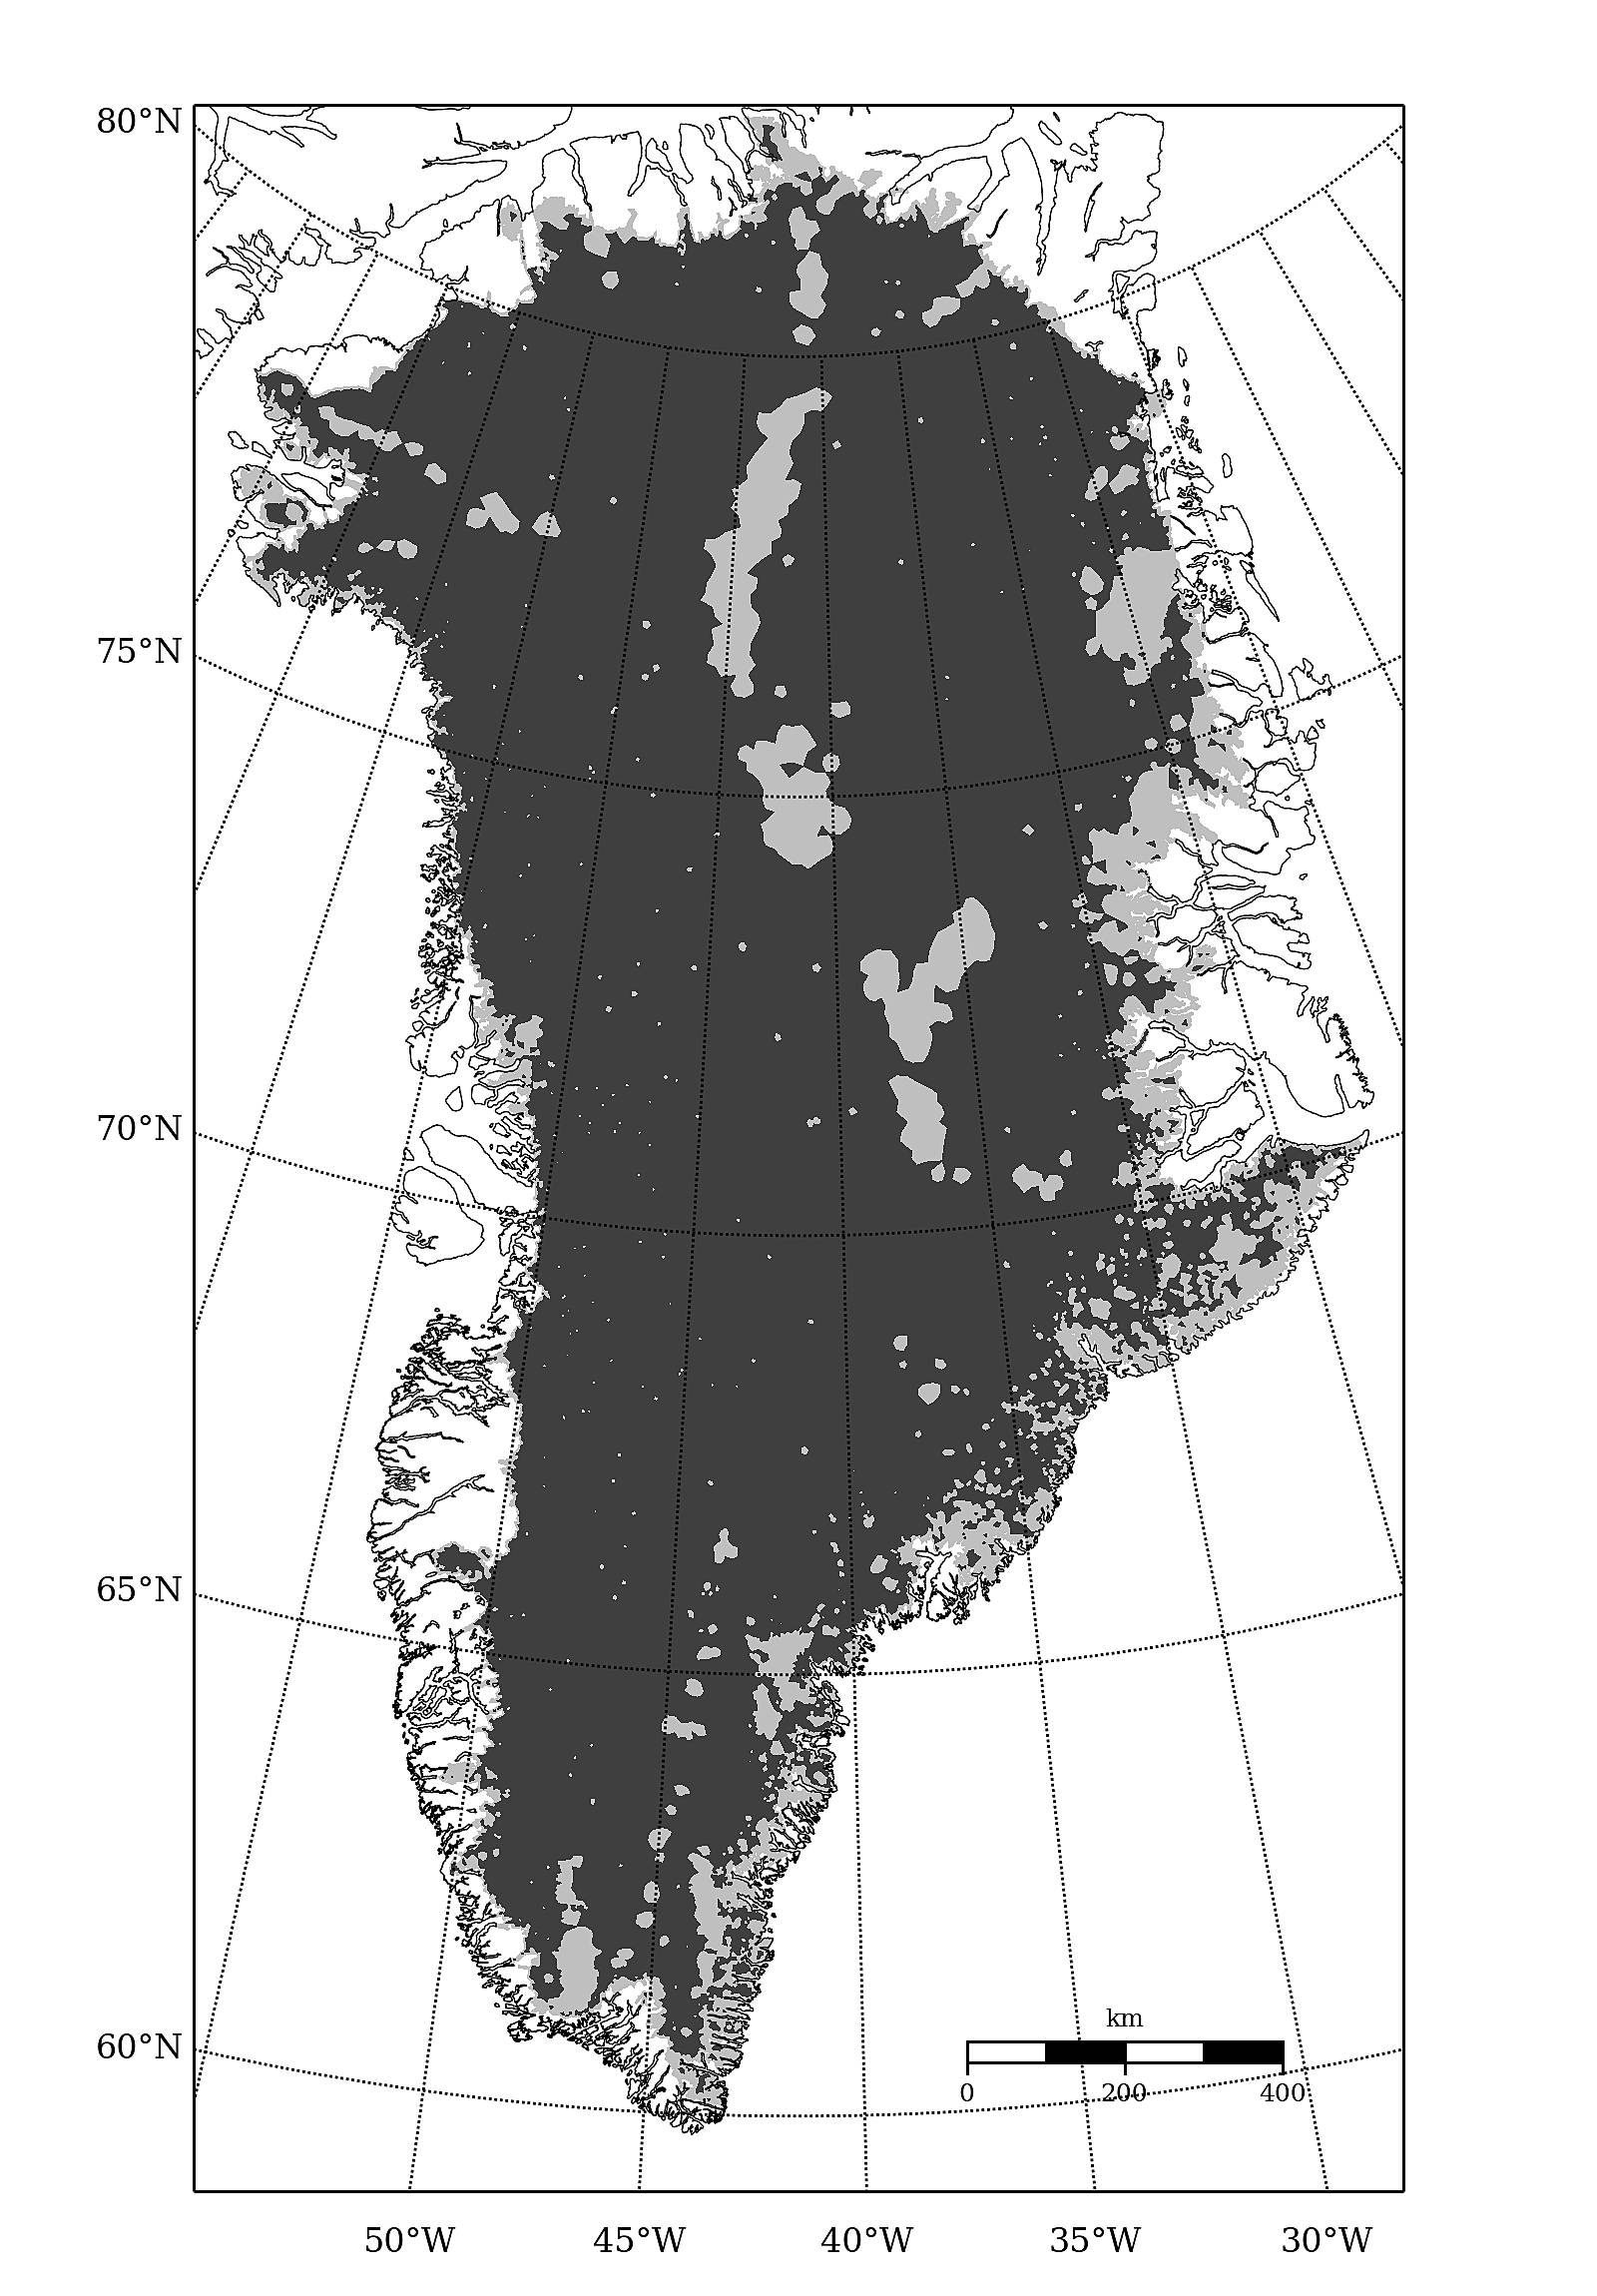
\includegraphics[width=0.35\textwidth]{images/greenland/stats/valid.jpg}
  \caption[]{Region of validity (darker region).}
\end{figure}

\begin{figure}
  \centering
  \begin{minipage}[b]{0.47\linewidth}
    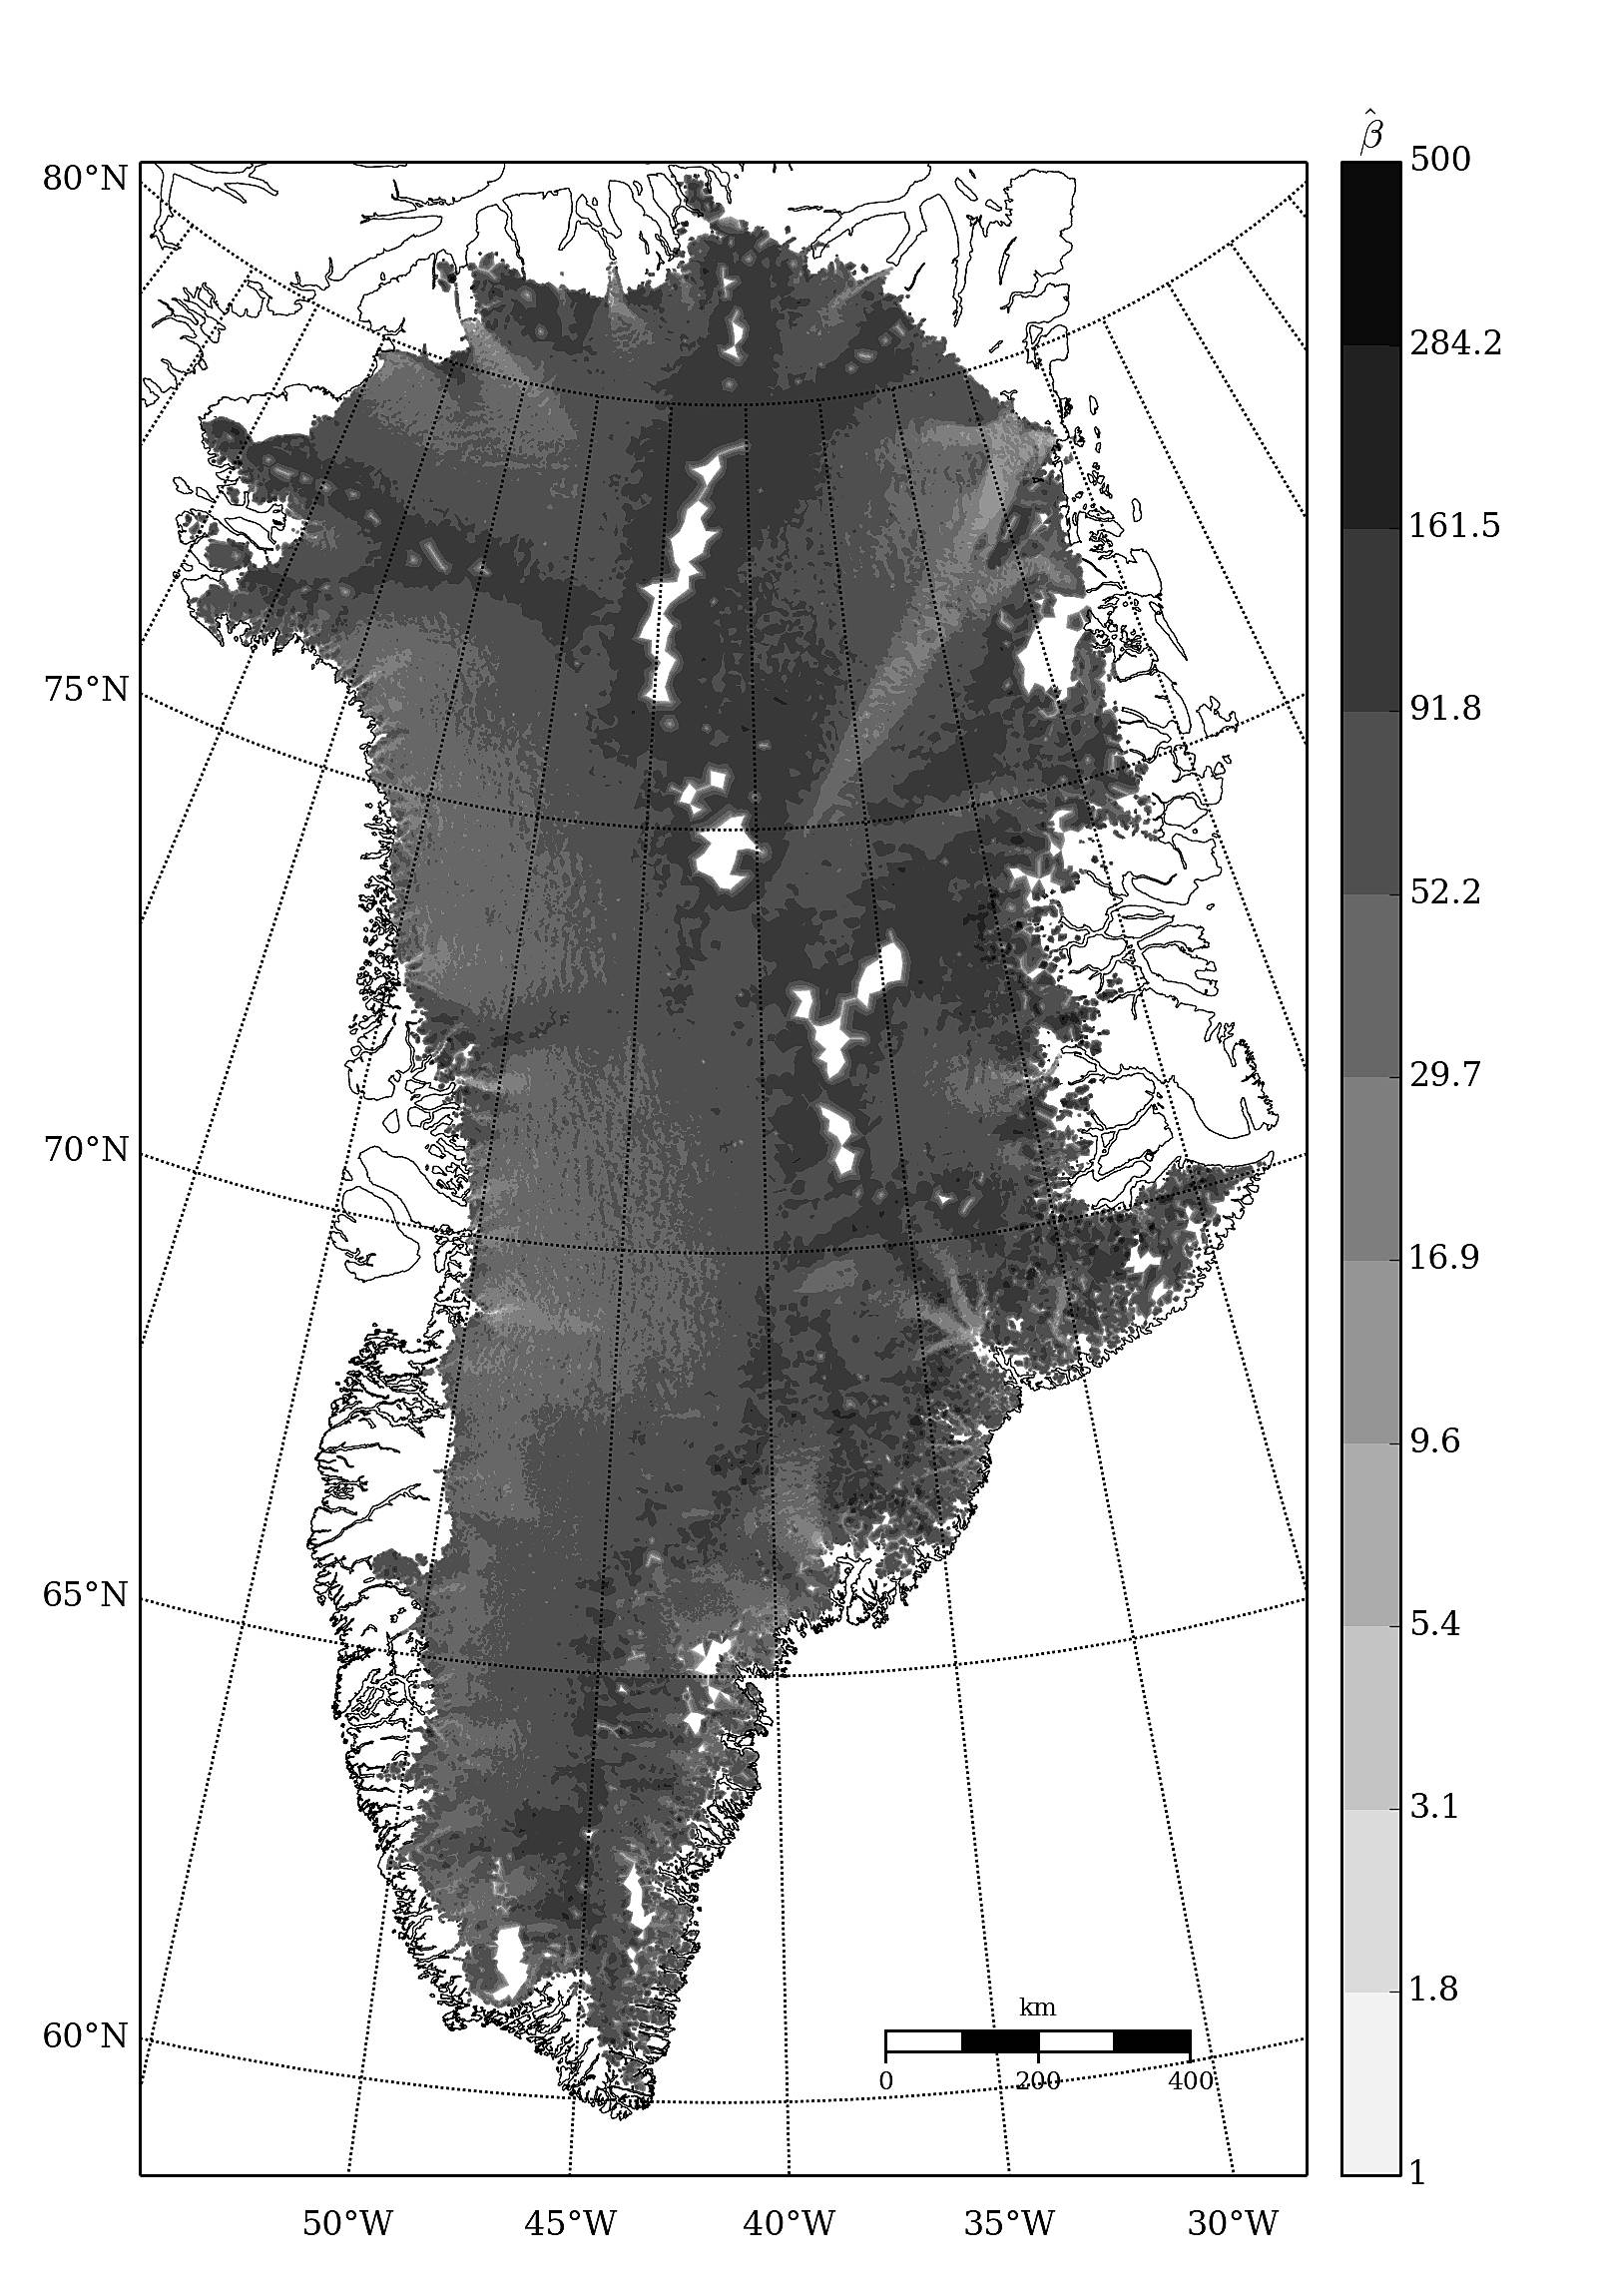
\includegraphics[width=1.0\textwidth]{images/greenland/stats/GLM_beta_no_uvw.jpg}
  \end{minipage}
  \quad
  \begin{minipage}[b]{0.47\linewidth}
    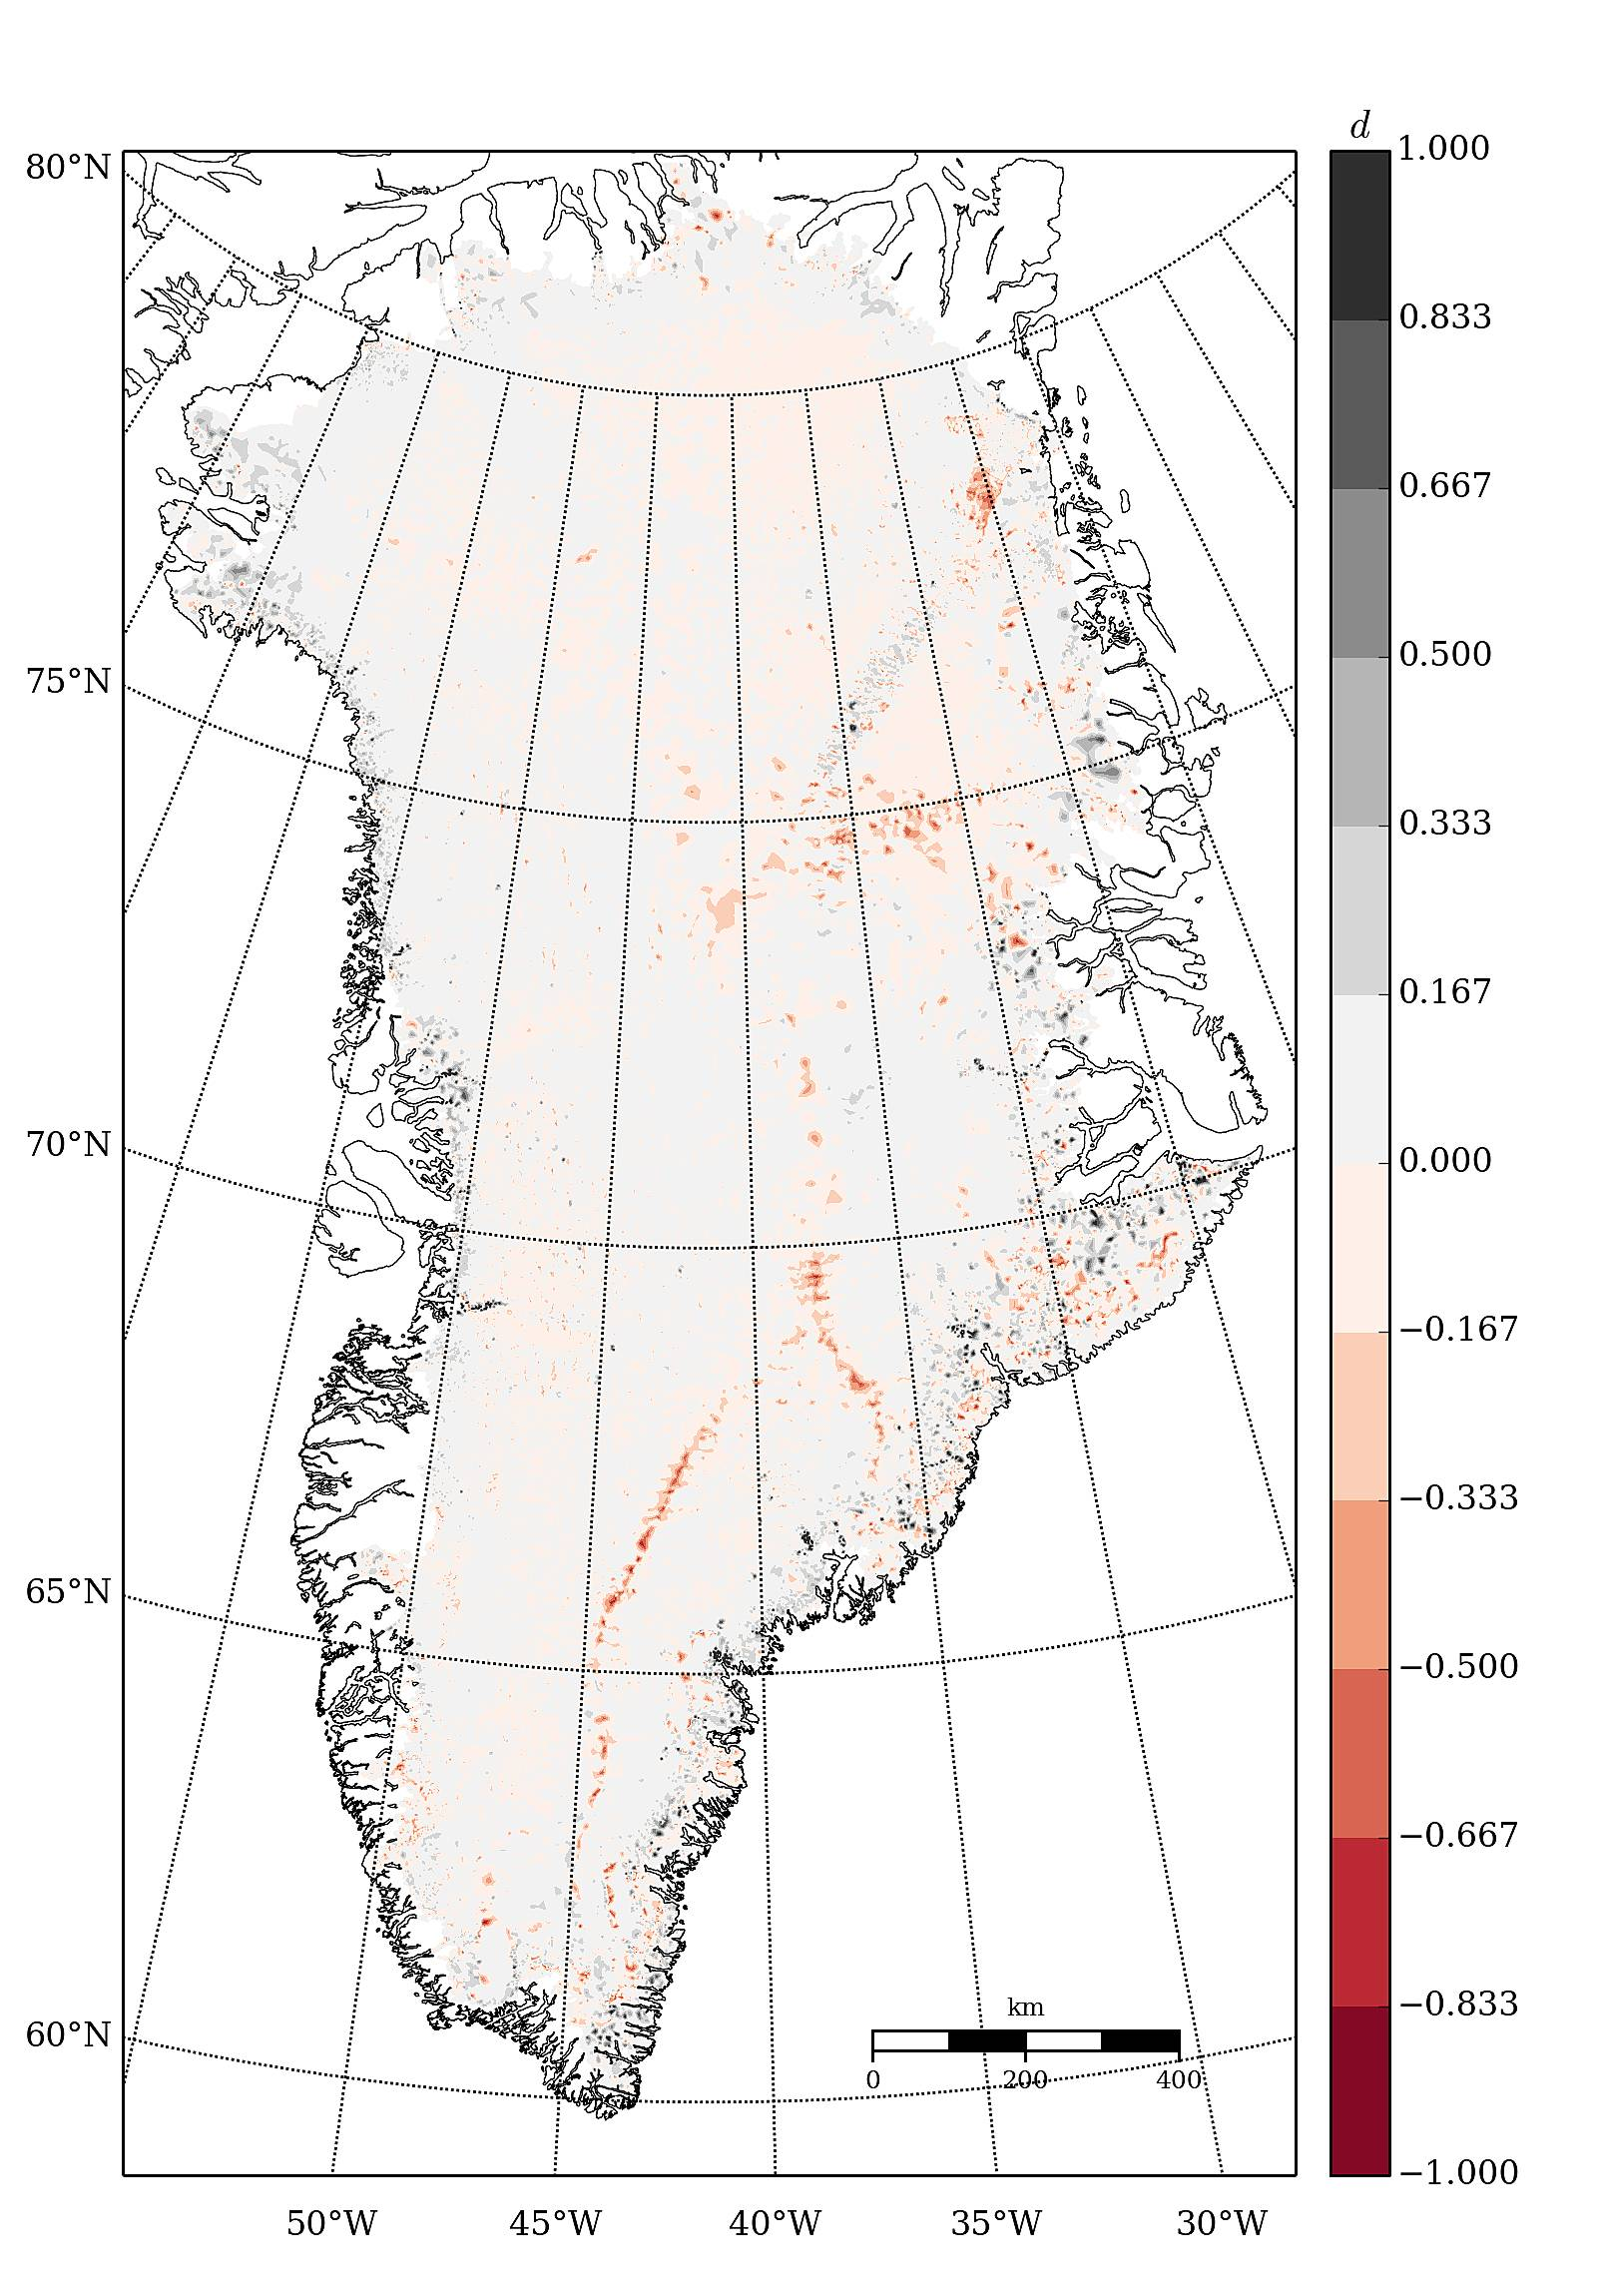
\includegraphics[width=1.0\textwidth]{images/greenland/stats/GLM_resid_no_uvw.jpg}
  \end{minipage}
  \begin{minipage}[b]{0.99\linewidth}
    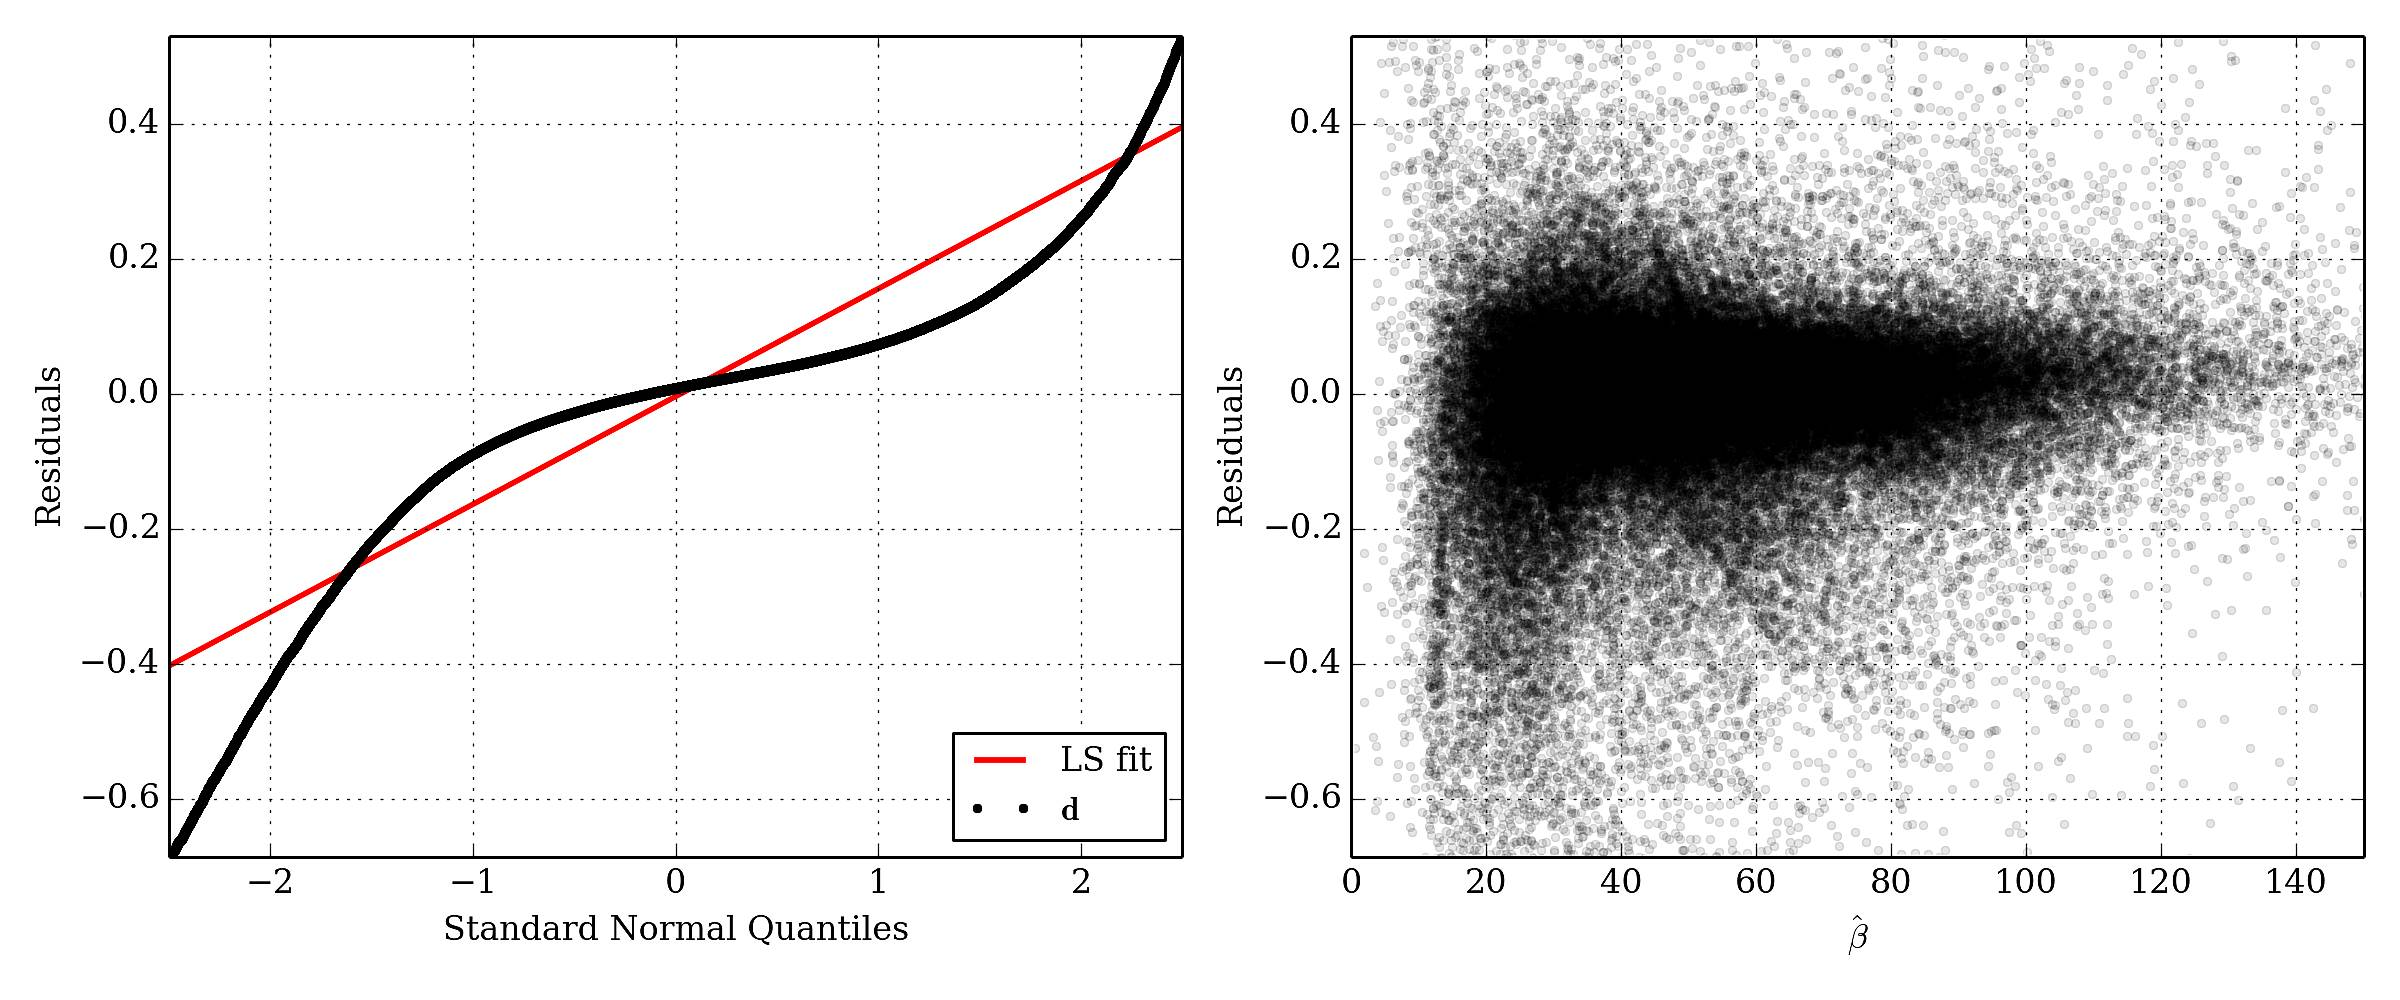
\includegraphics[width=1.0\textwidth]{images/greenland/stats/GLM_resid-NQ_no_uvw.jpg}
  \end{minipage}
  \caption[]{GLM model fit $\bm{\hat{\beta}}$ and residual $\mathbf{d}$ for the full design matrix $\mat{X}$.}
\end{figure}

\begin{figure}
  \centering
  \begin{minipage}[b]{0.47\linewidth}
    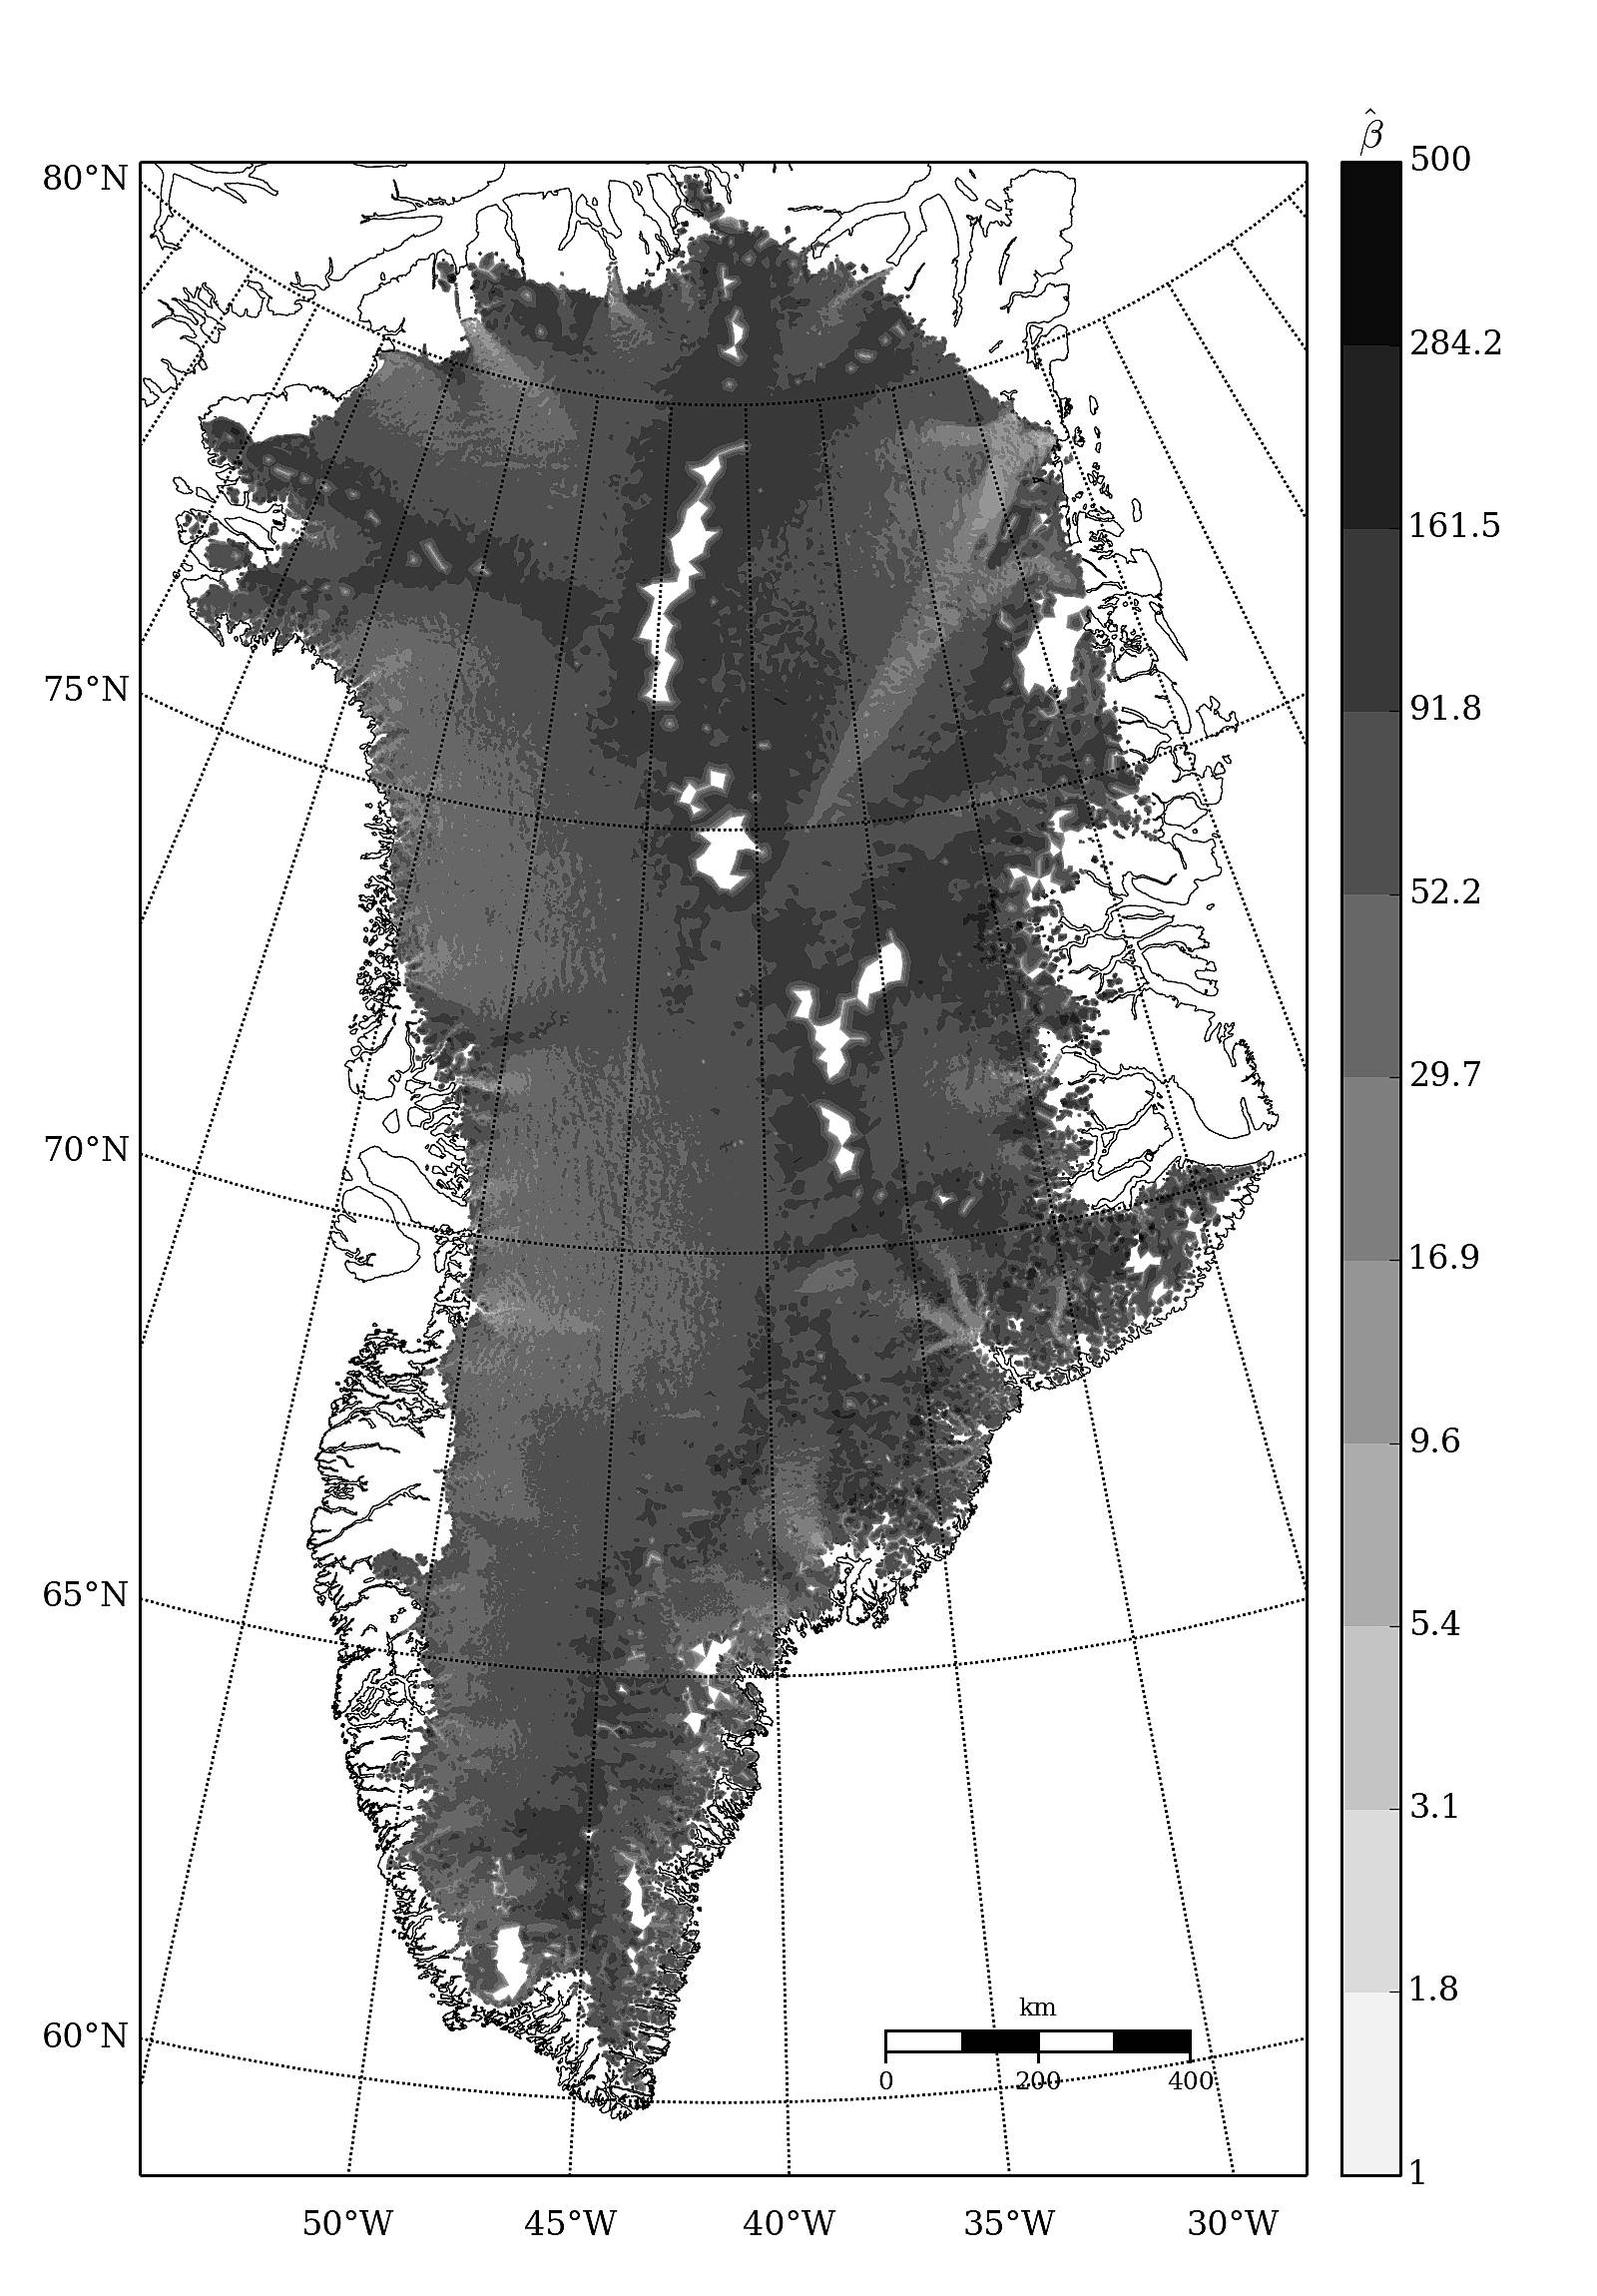
\includegraphics[width=1.0\textwidth]{images/greenland/stats/GLM_beta_no_Mb.jpg}
  \end{minipage}
  \quad
  \begin{minipage}[b]{0.47\linewidth}
    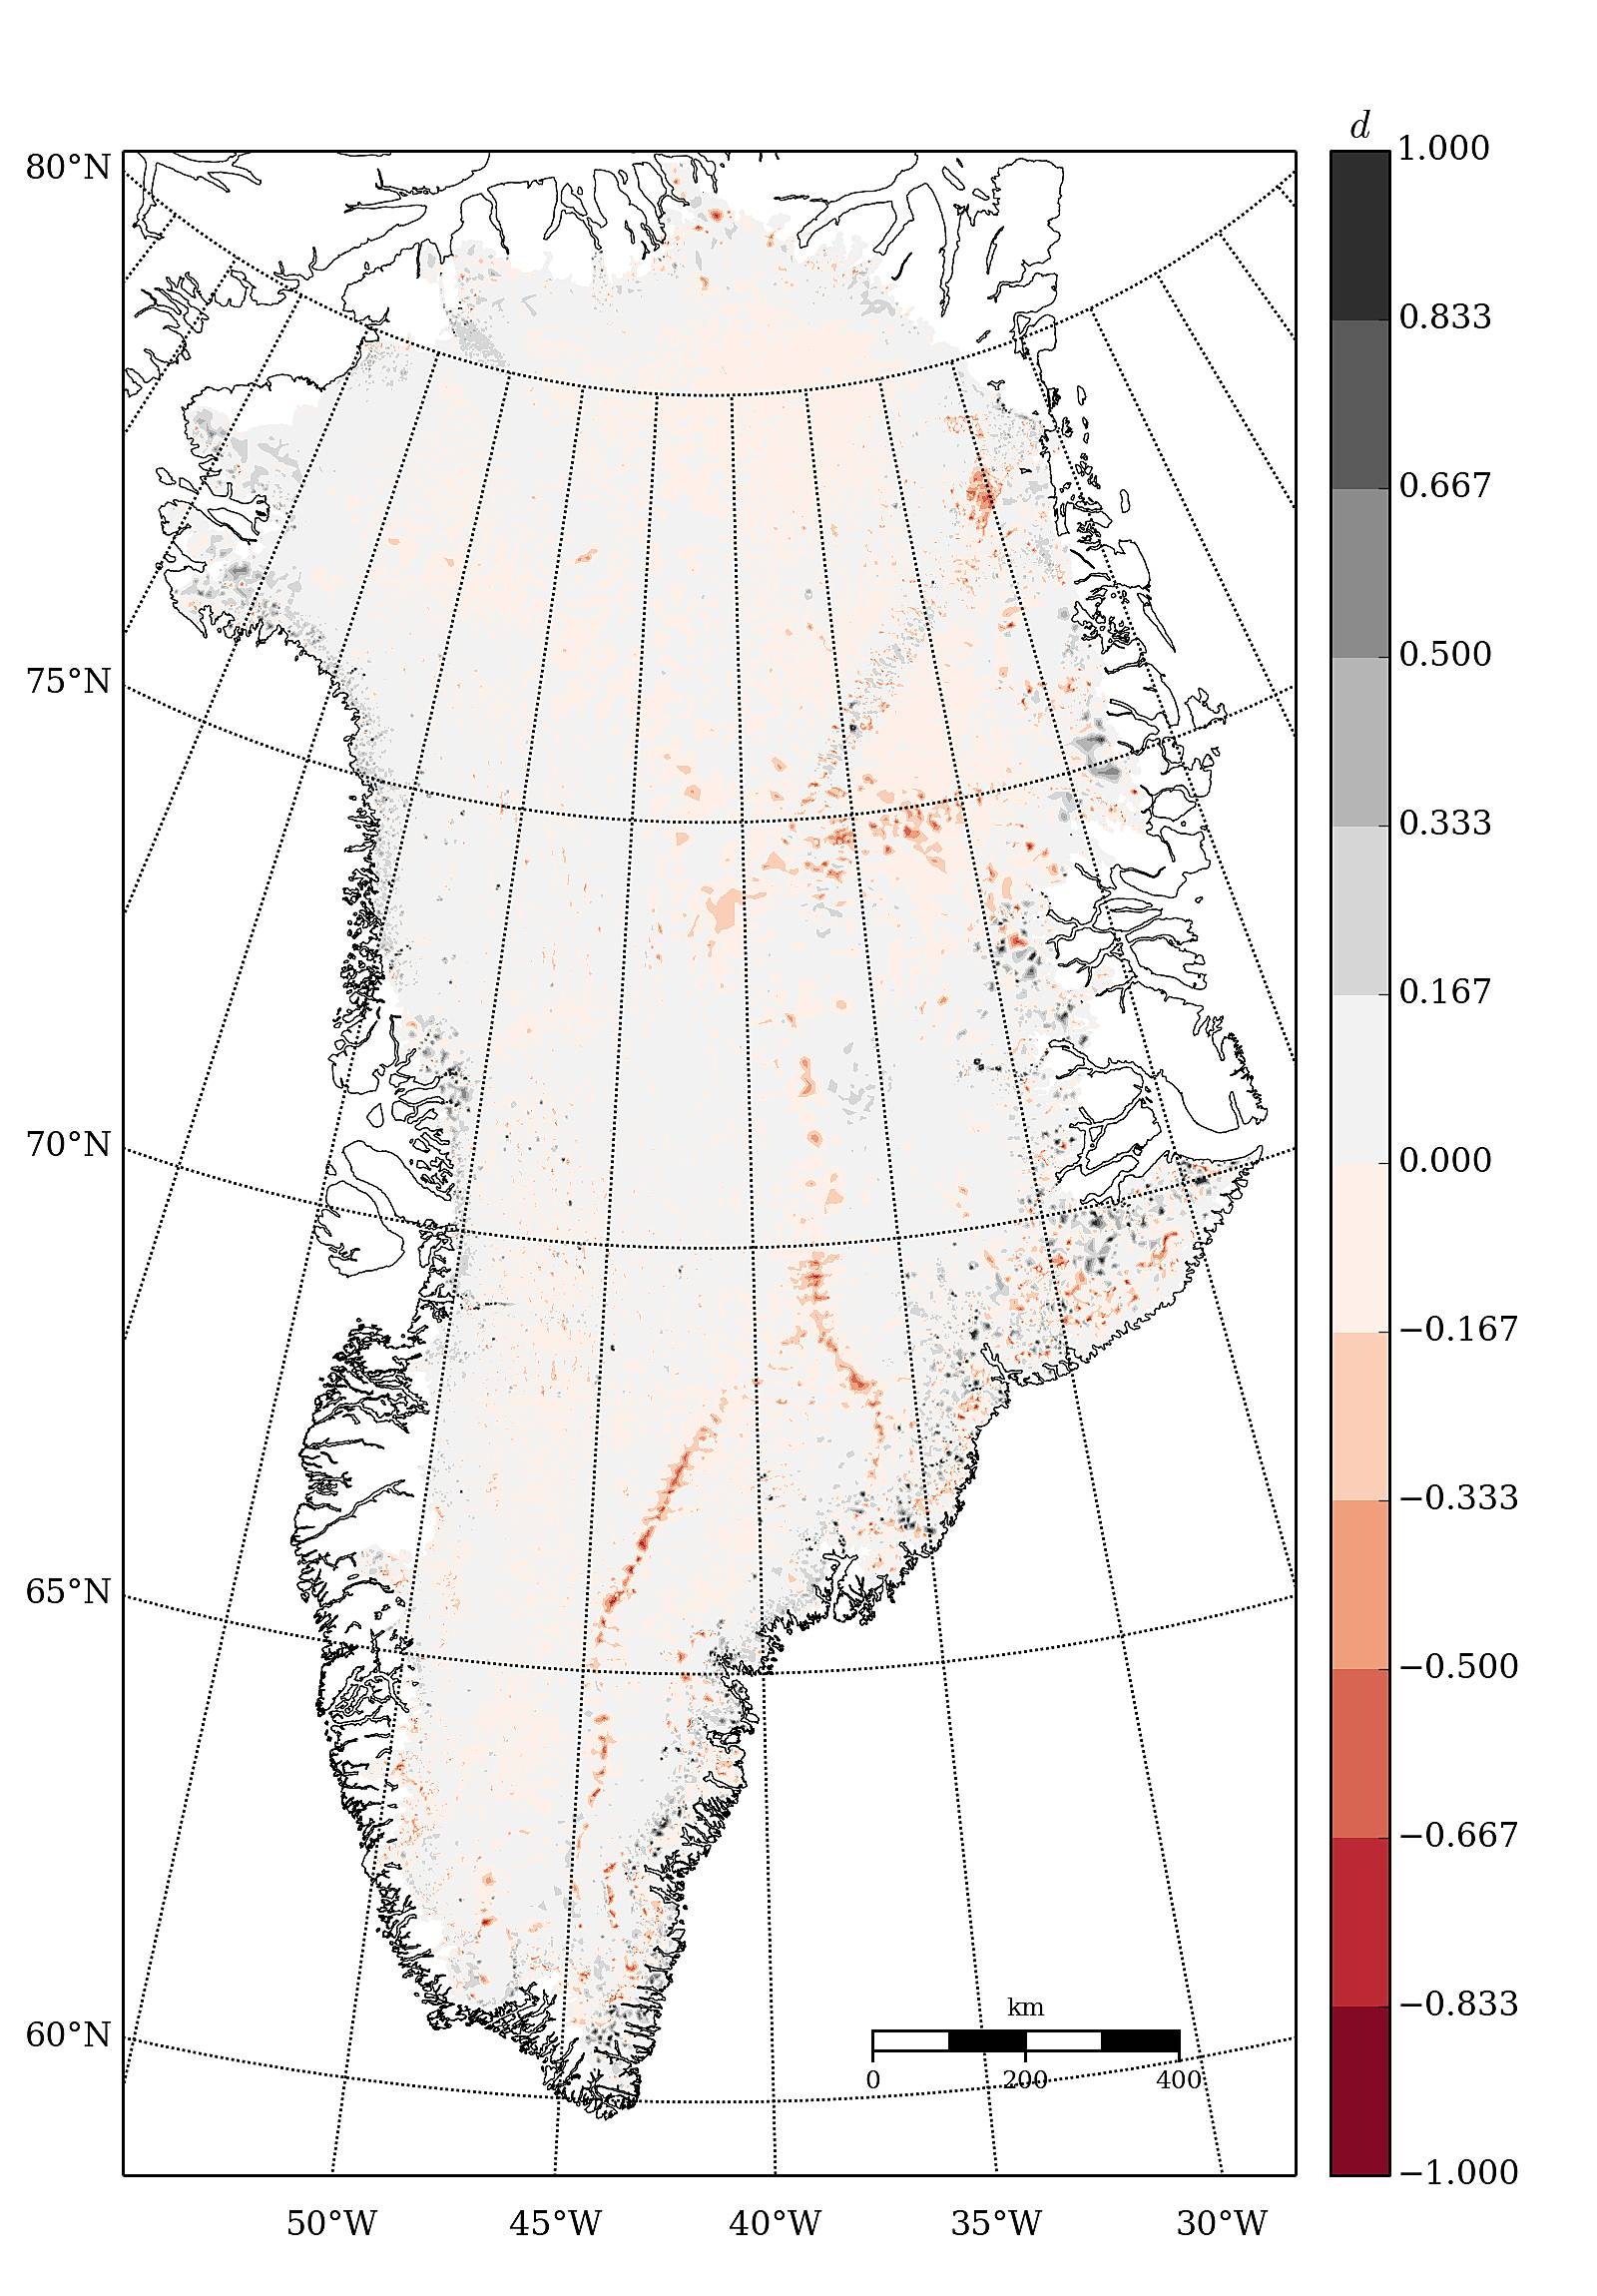
\includegraphics[width=1.0\textwidth]{images/greenland/stats/GLM_resid_no_Mb.jpg}
  \end{minipage}
  \begin{minipage}[b]{0.99\linewidth}
    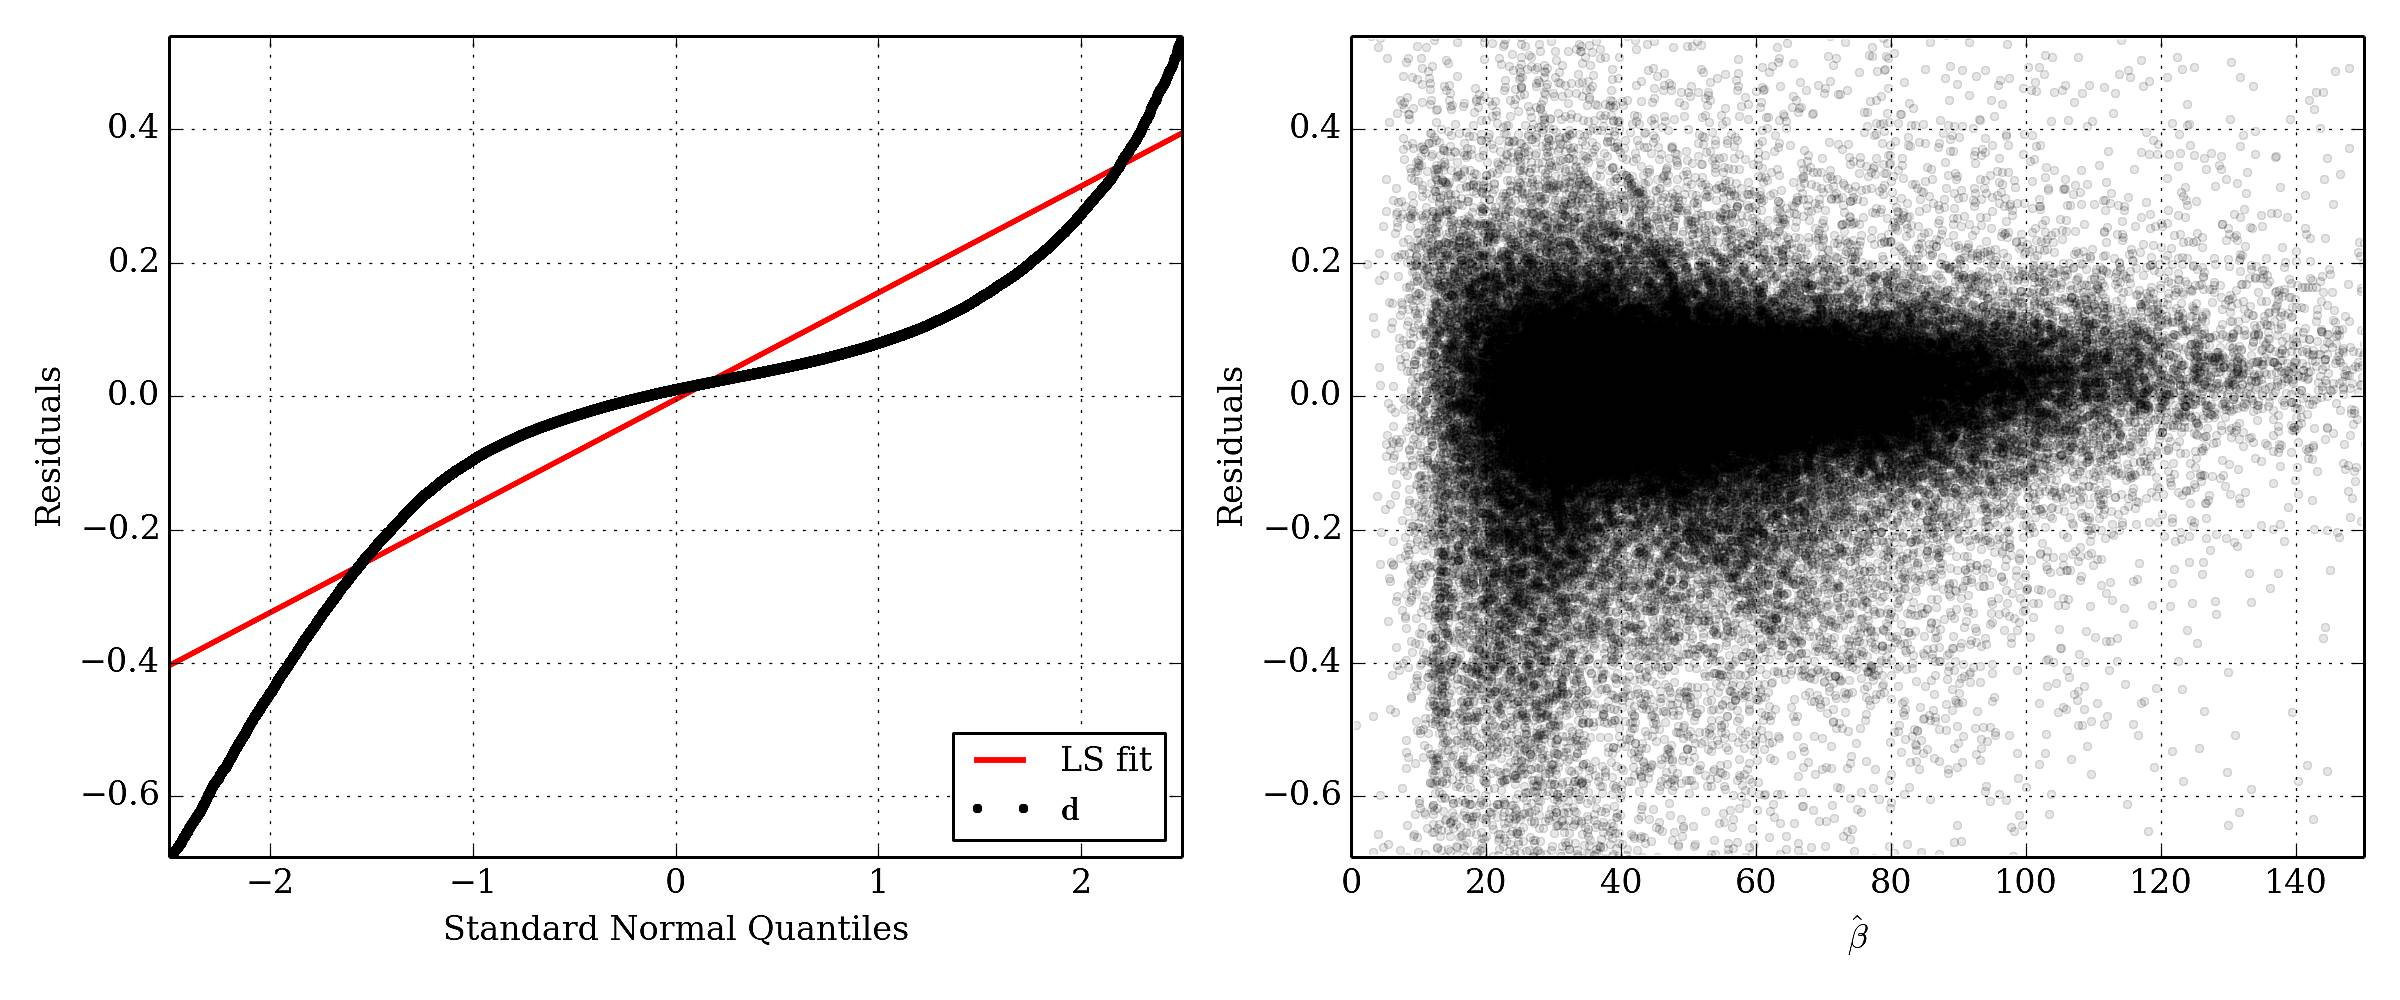
\includegraphics[width=1.0\textwidth]{images/greenland/stats/GLM_resid-NQ_no_Mb.jpg}
  \end{minipage}
  \caption[]{GLM model fit $\bm{\hat{\beta}}$ and residual $\mathbf{d}$, excluding $M_B$ from $\mat{X}$.}
\end{figure}

\begin{figure}
  \centering
  \begin{minipage}[b]{0.47\linewidth}
    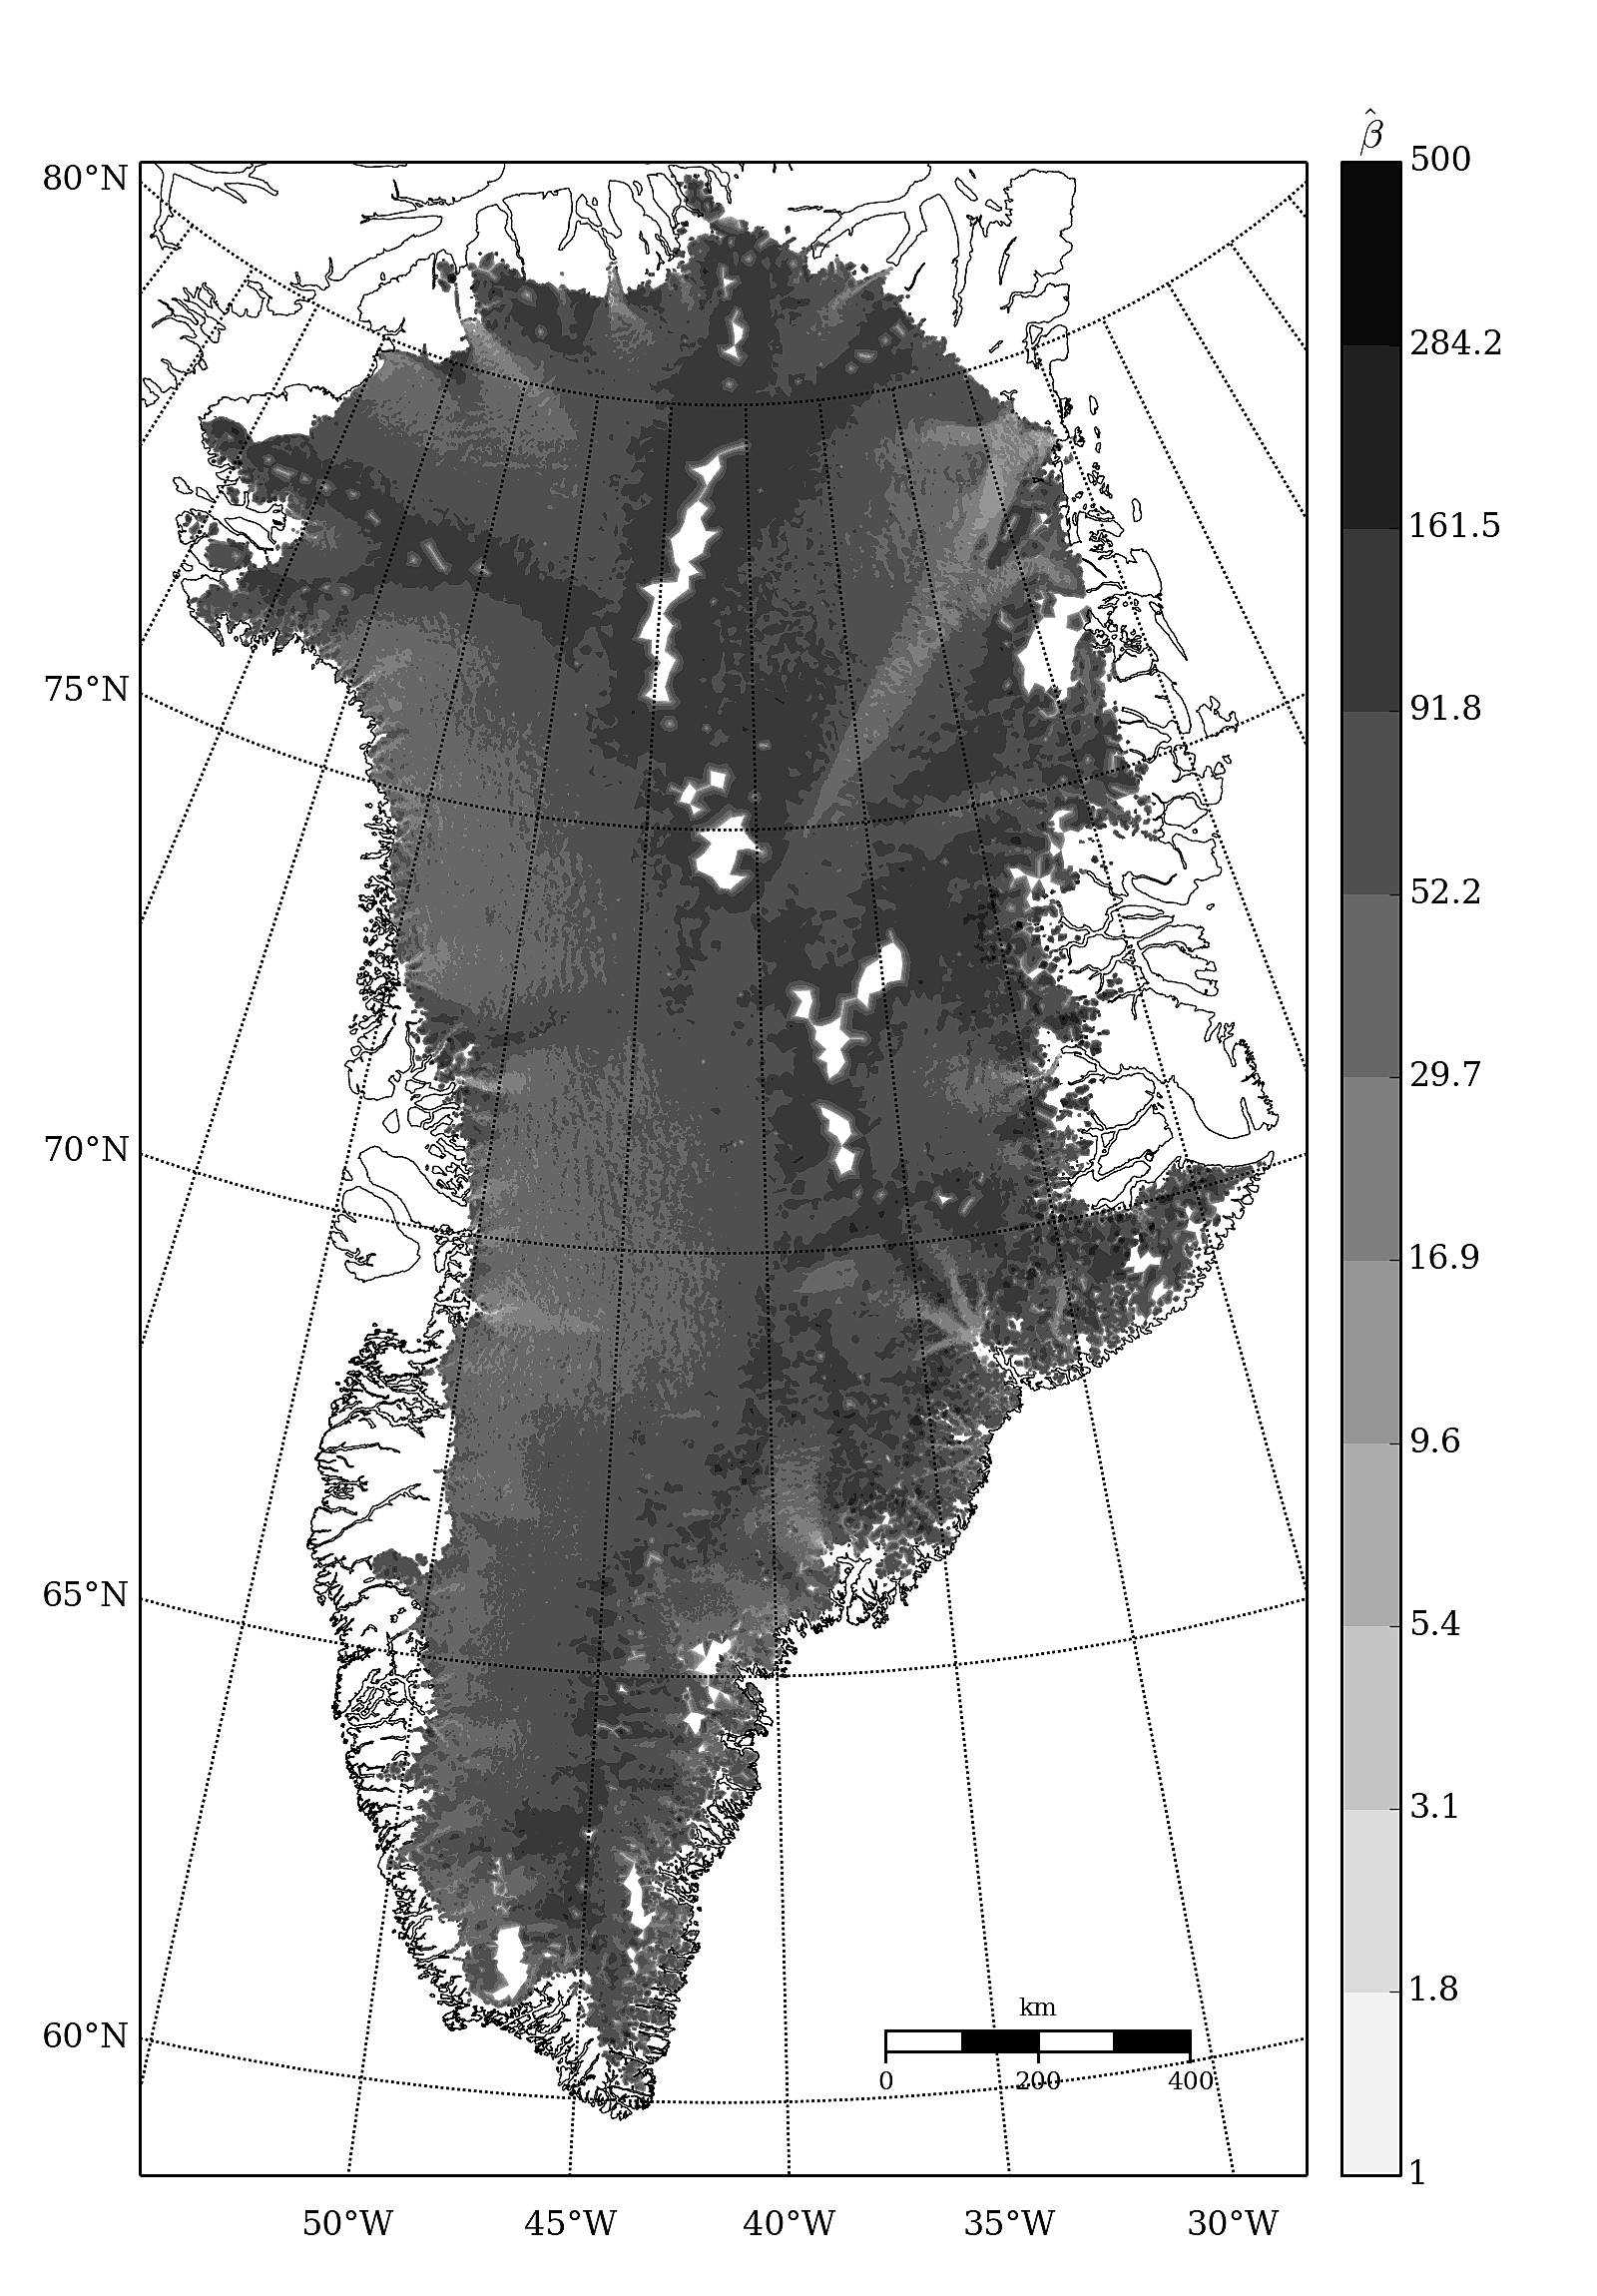
\includegraphics[width=1.0\textwidth]{images/greenland/stats/GLM_beta_no_T.jpg}
  \end{minipage}
  \quad
  \begin{minipage}[b]{0.47\linewidth}
    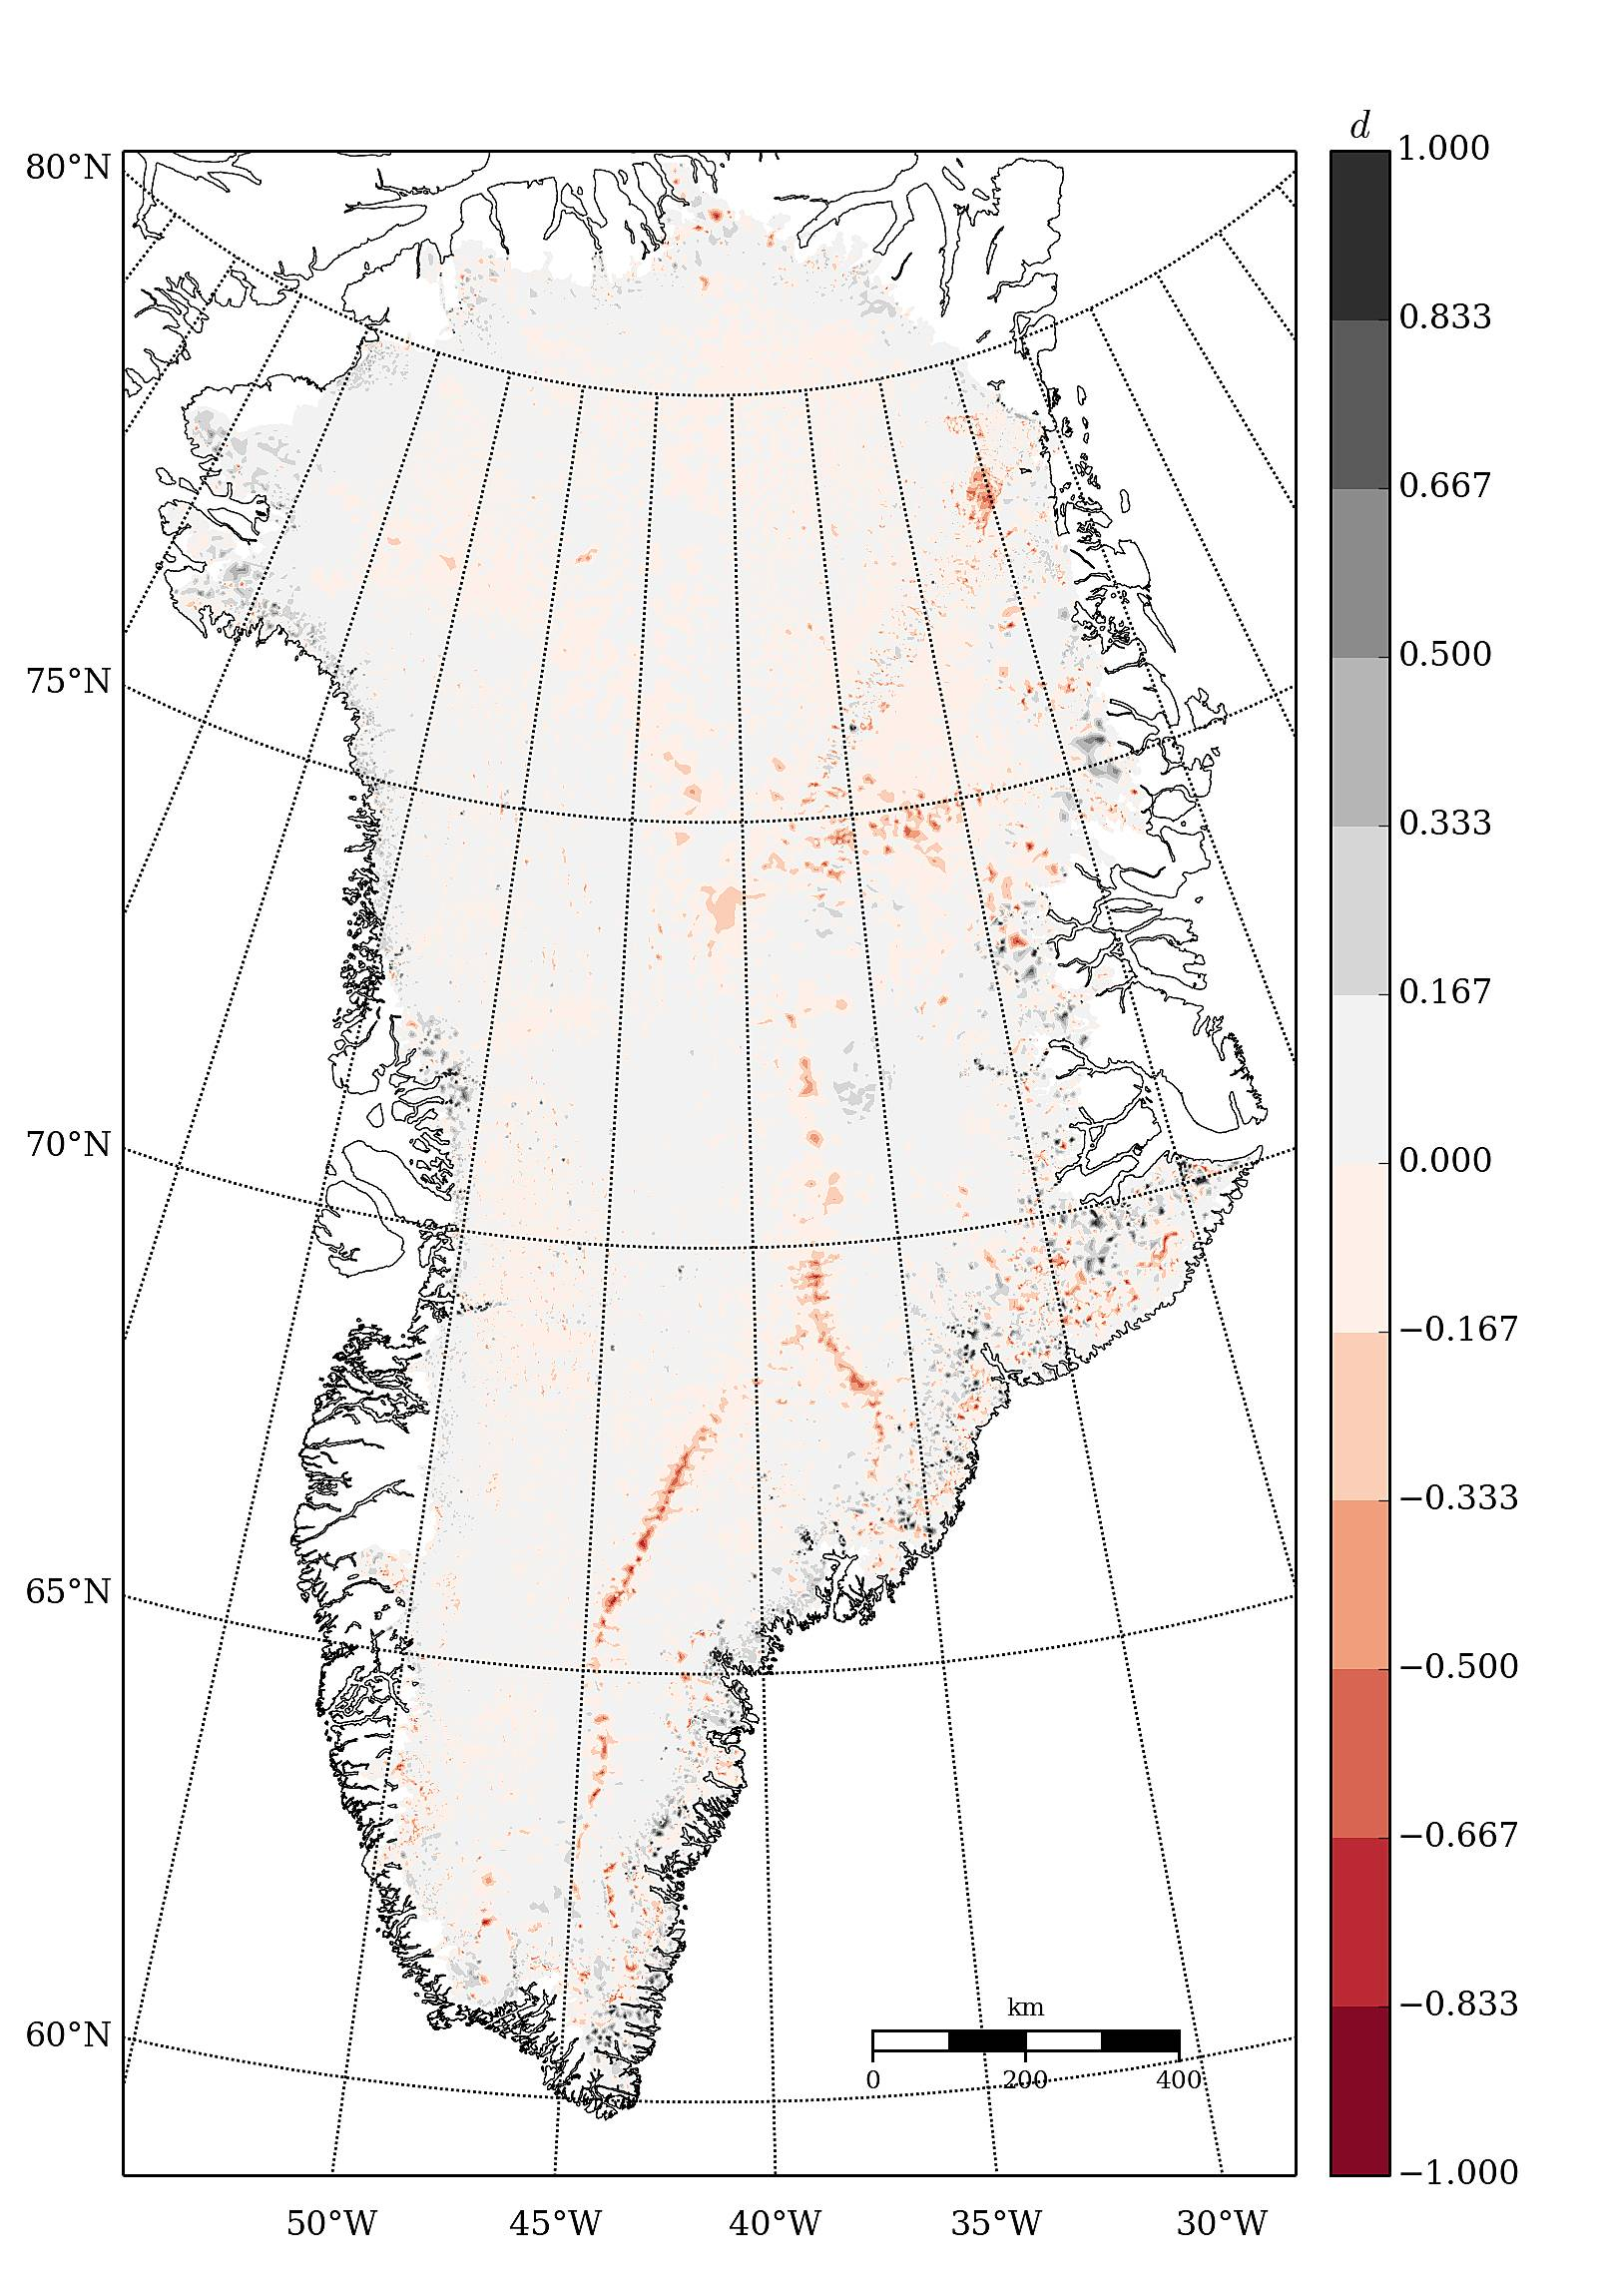
\includegraphics[width=1.0\textwidth]{images/greenland/stats/GLM_resid_no_T.jpg}
  \end{minipage}
  \begin{minipage}[b]{0.99\linewidth}
    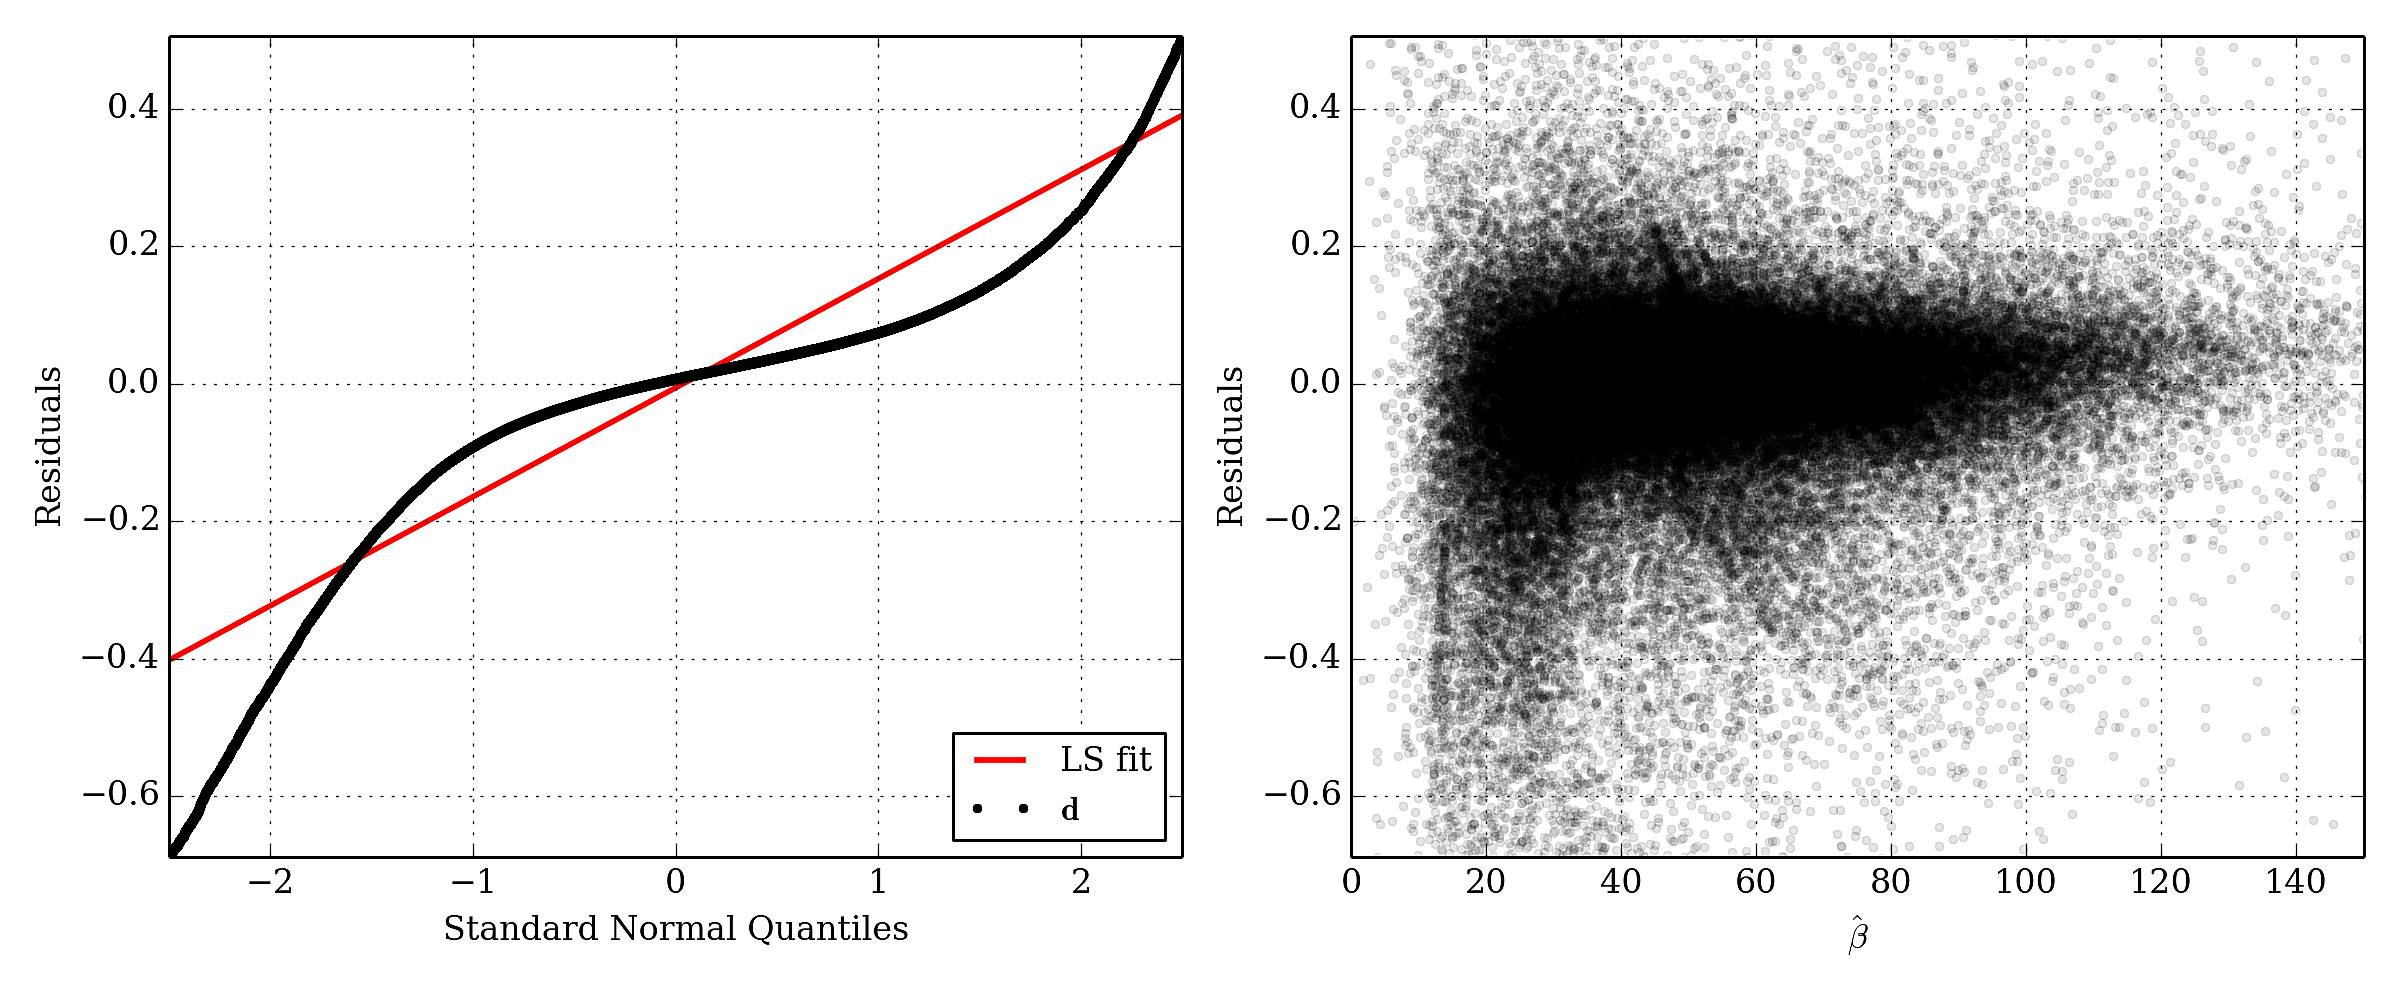
\includegraphics[width=1.0\textwidth]{images/greenland/stats/GLM_resid-NQ_no_T.jpg}
  \end{minipage}
  \caption[]{GLM model fit $\bm{\hat{\beta}}$ and residual $\mathbf{d}$, excluding $T_B$ from $\mat{X}$.}
\end{figure}

\begin{figure}
  \centering
  \begin{minipage}[b]{0.47\linewidth}
    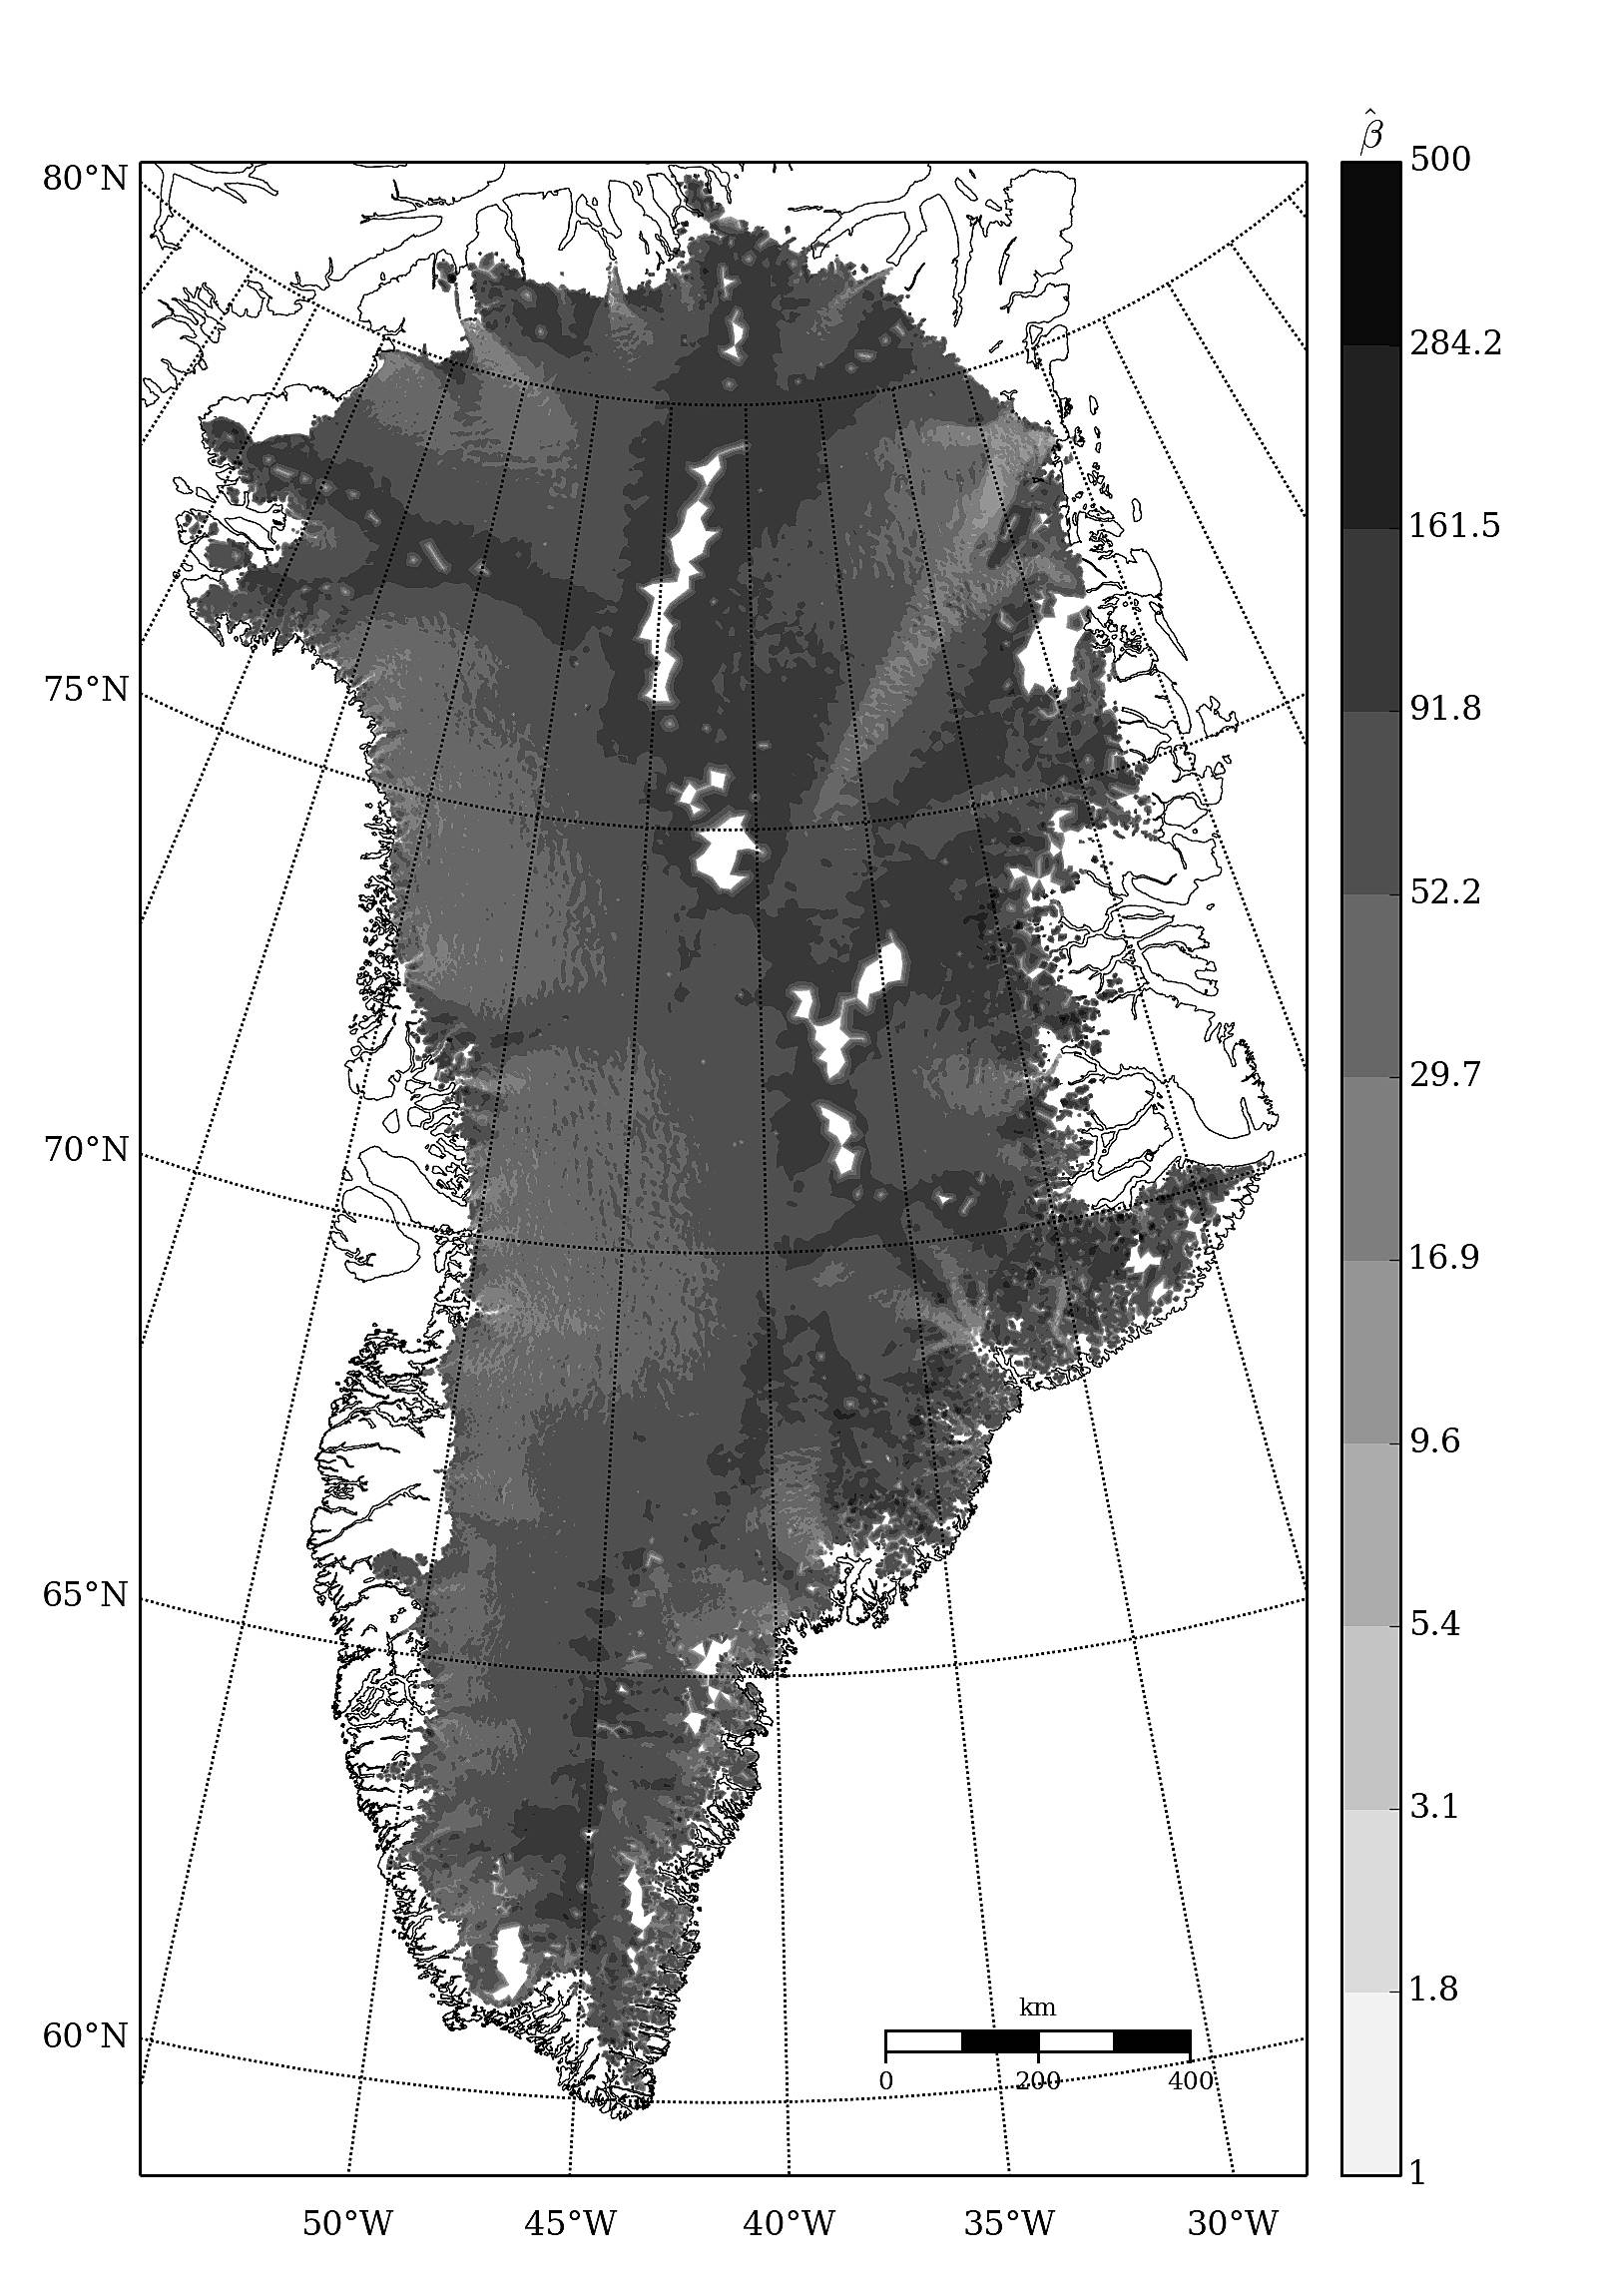
\includegraphics[width=1.0\textwidth]{images/greenland/stats/GLM_beta_no_membrane_stress.jpg}
  \end{minipage}
  \quad
  \begin{minipage}[b]{0.47\linewidth}
    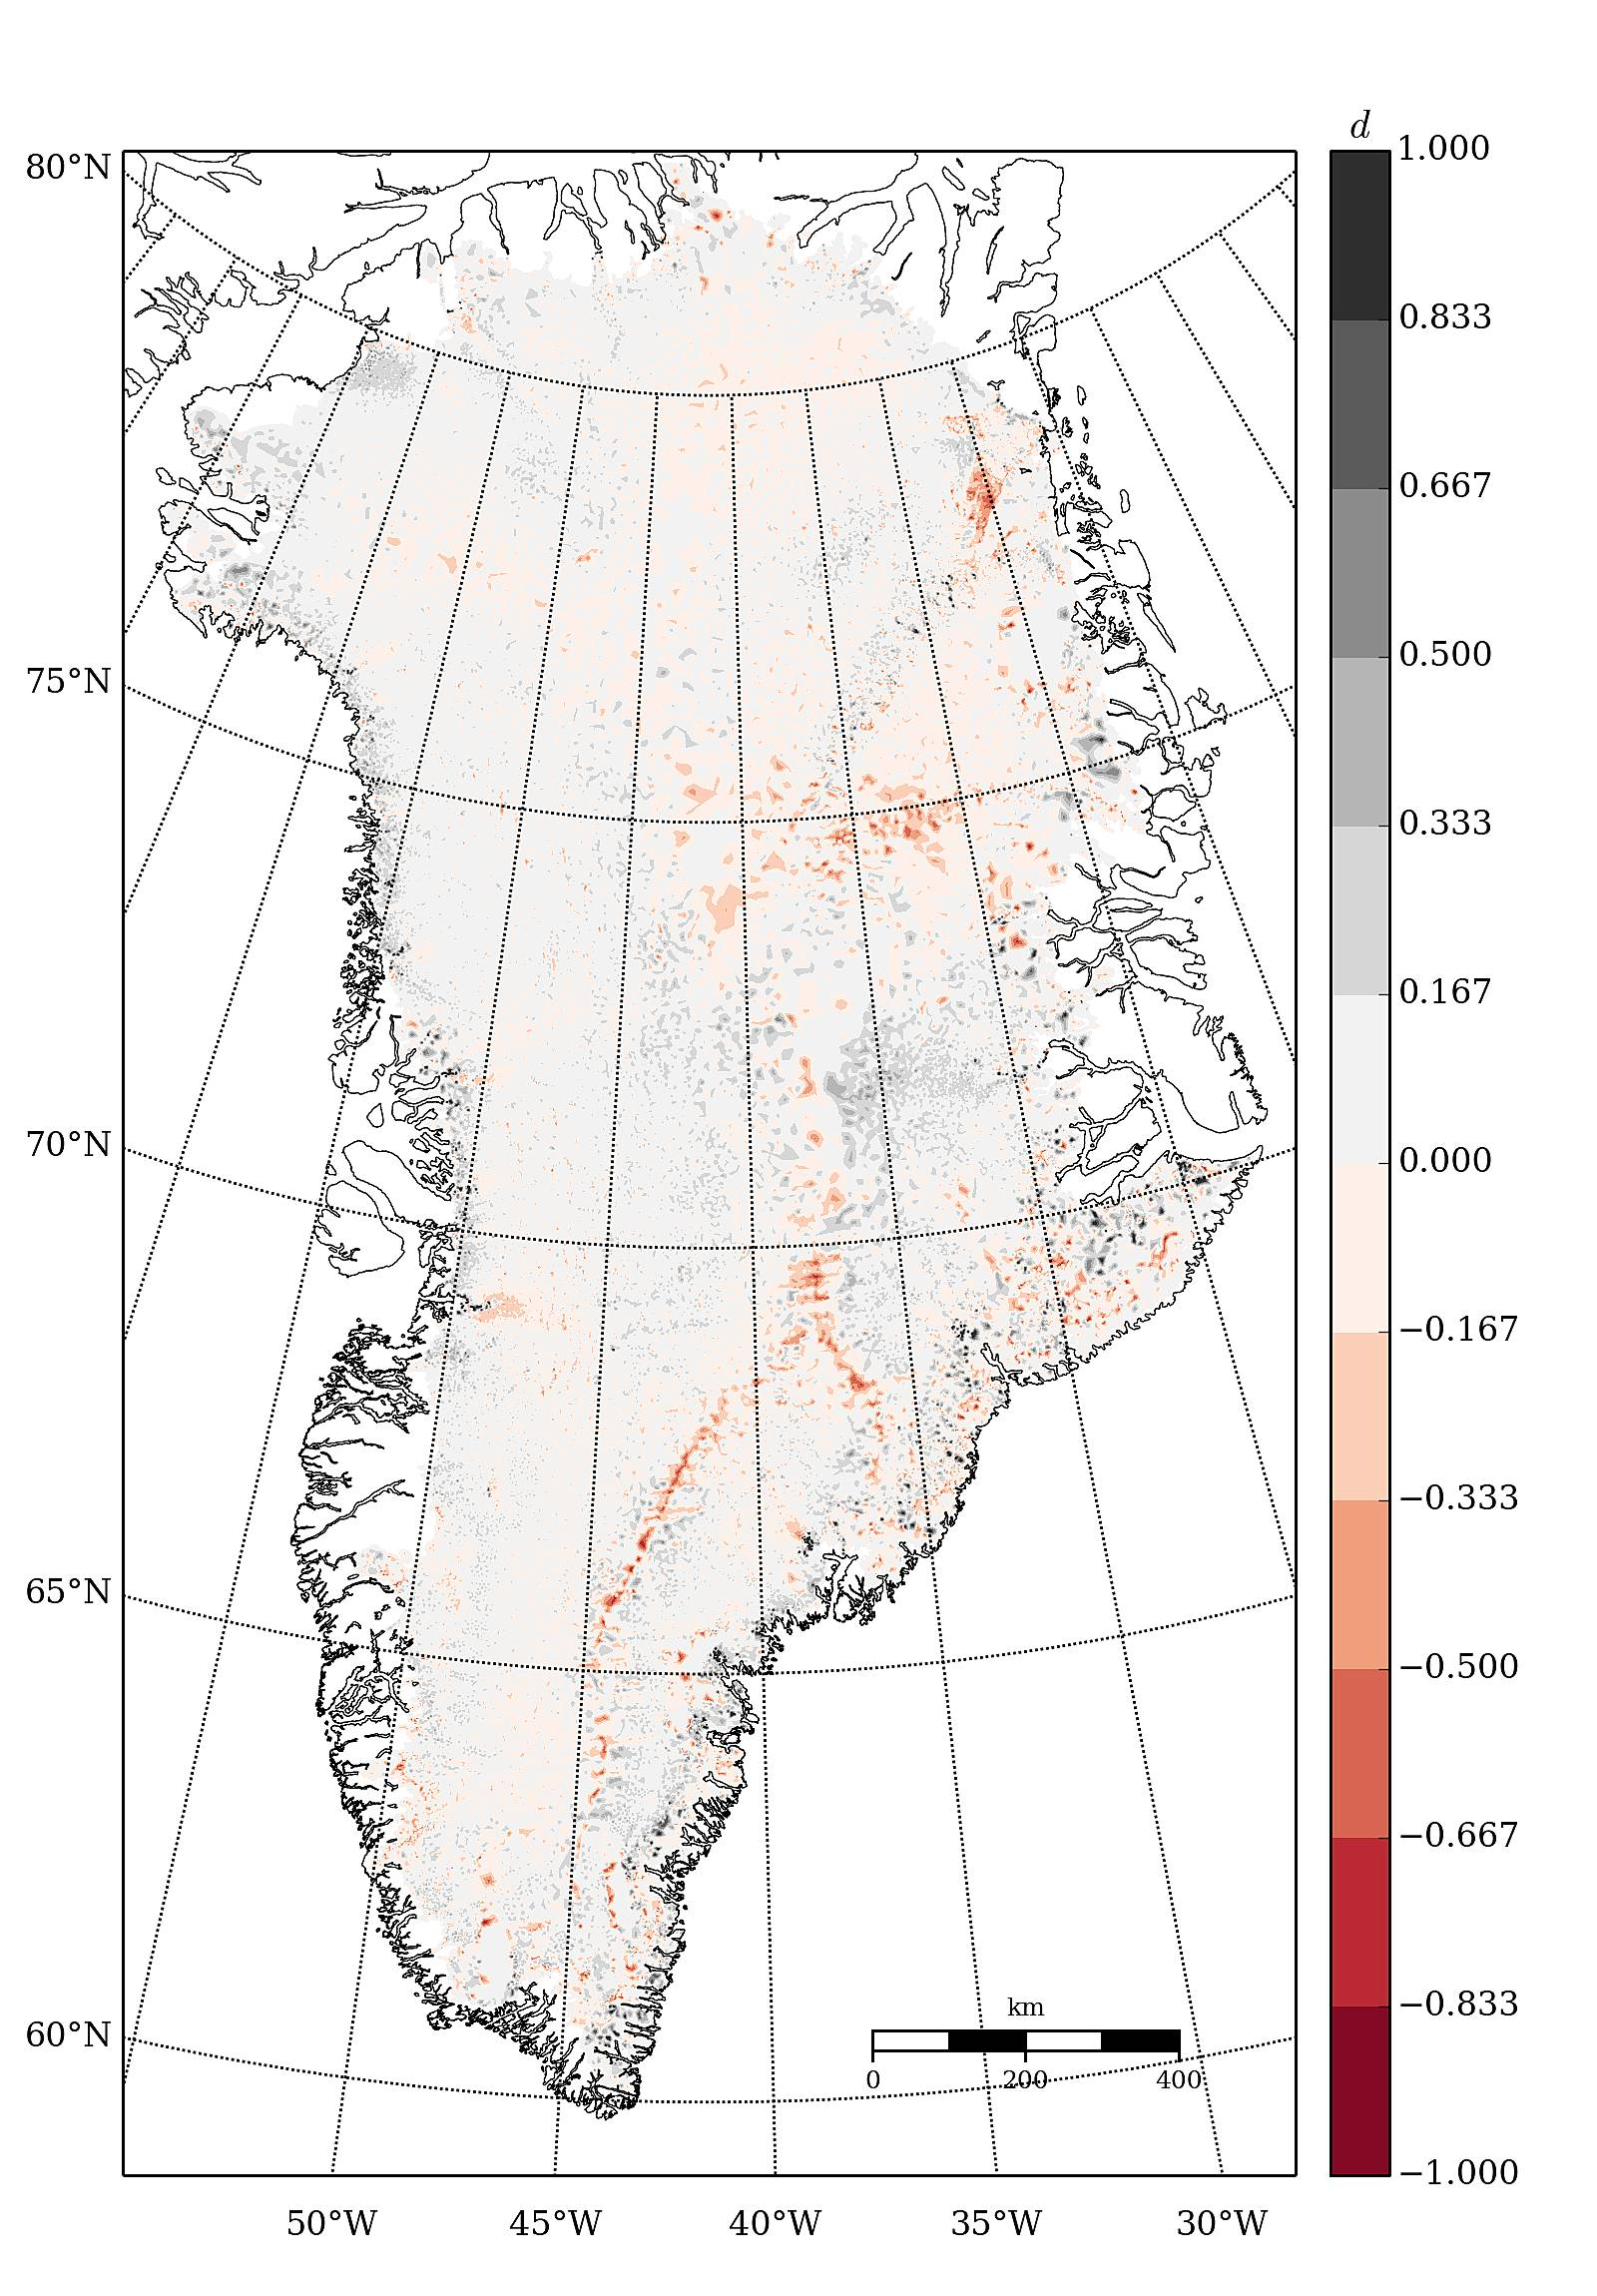
\includegraphics[width=1.0\textwidth]{images/greenland/stats/GLM_resid_no_membrane_stress.jpg}
  \end{minipage}
  \begin{minipage}[b]{0.99\linewidth}
    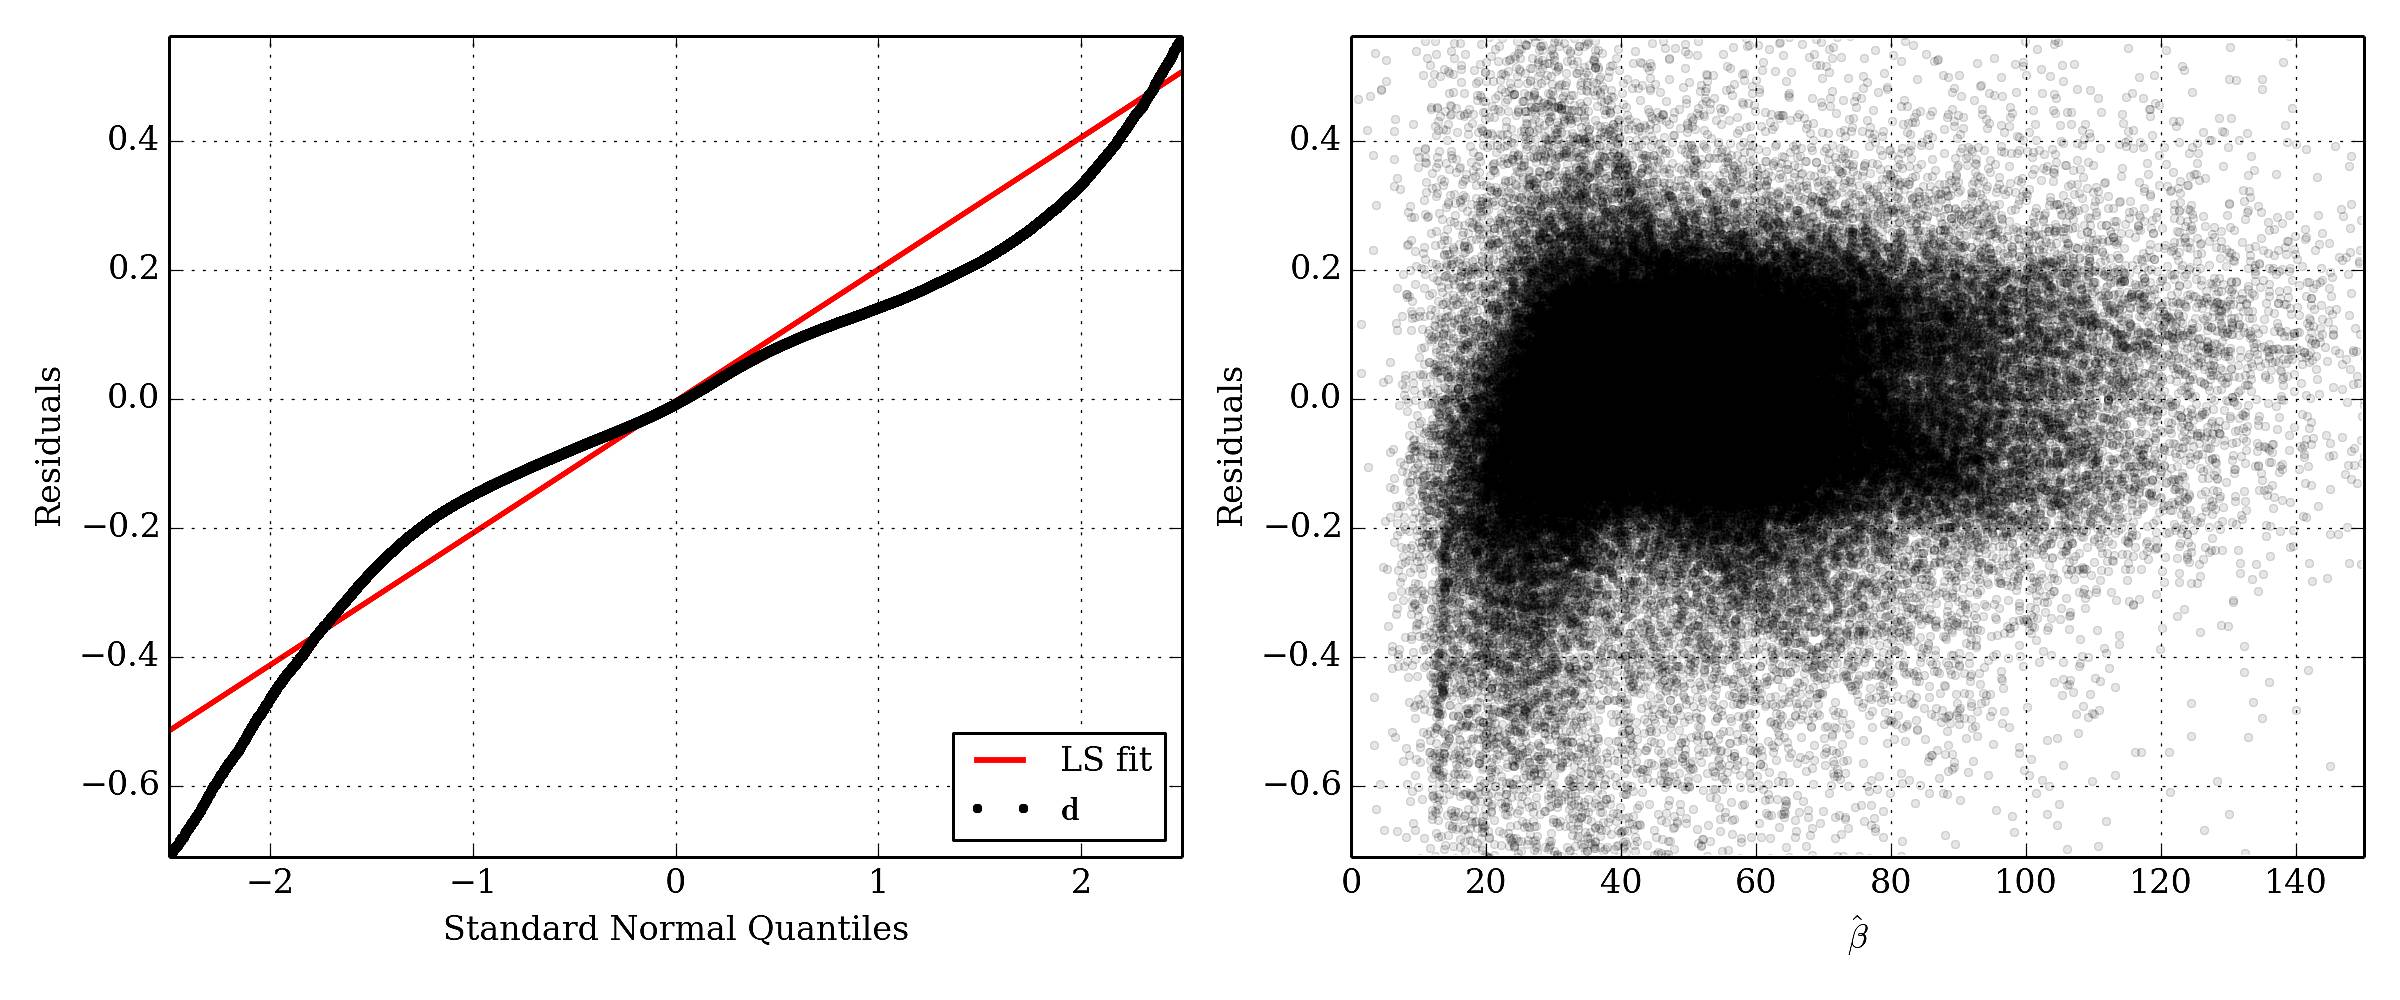
\includegraphics[width=1.0\textwidth]{images/greenland/stats/GLM_resid-NQ_no_membrane_stress.jpg}
  \end{minipage}
  \caption[]{GLM model fit $\bm{\hat{\beta}}$ and residual $\mathbf{d}$, excluding $\tau_{nn}$, $\tau_{nt}$, $\tau_{tn}$, and $\tau_{tt}$ from $\mat{X}$.}
\end{figure}

\begin{figure}
  \centering
  \begin{minipage}[b]{0.47\linewidth}
    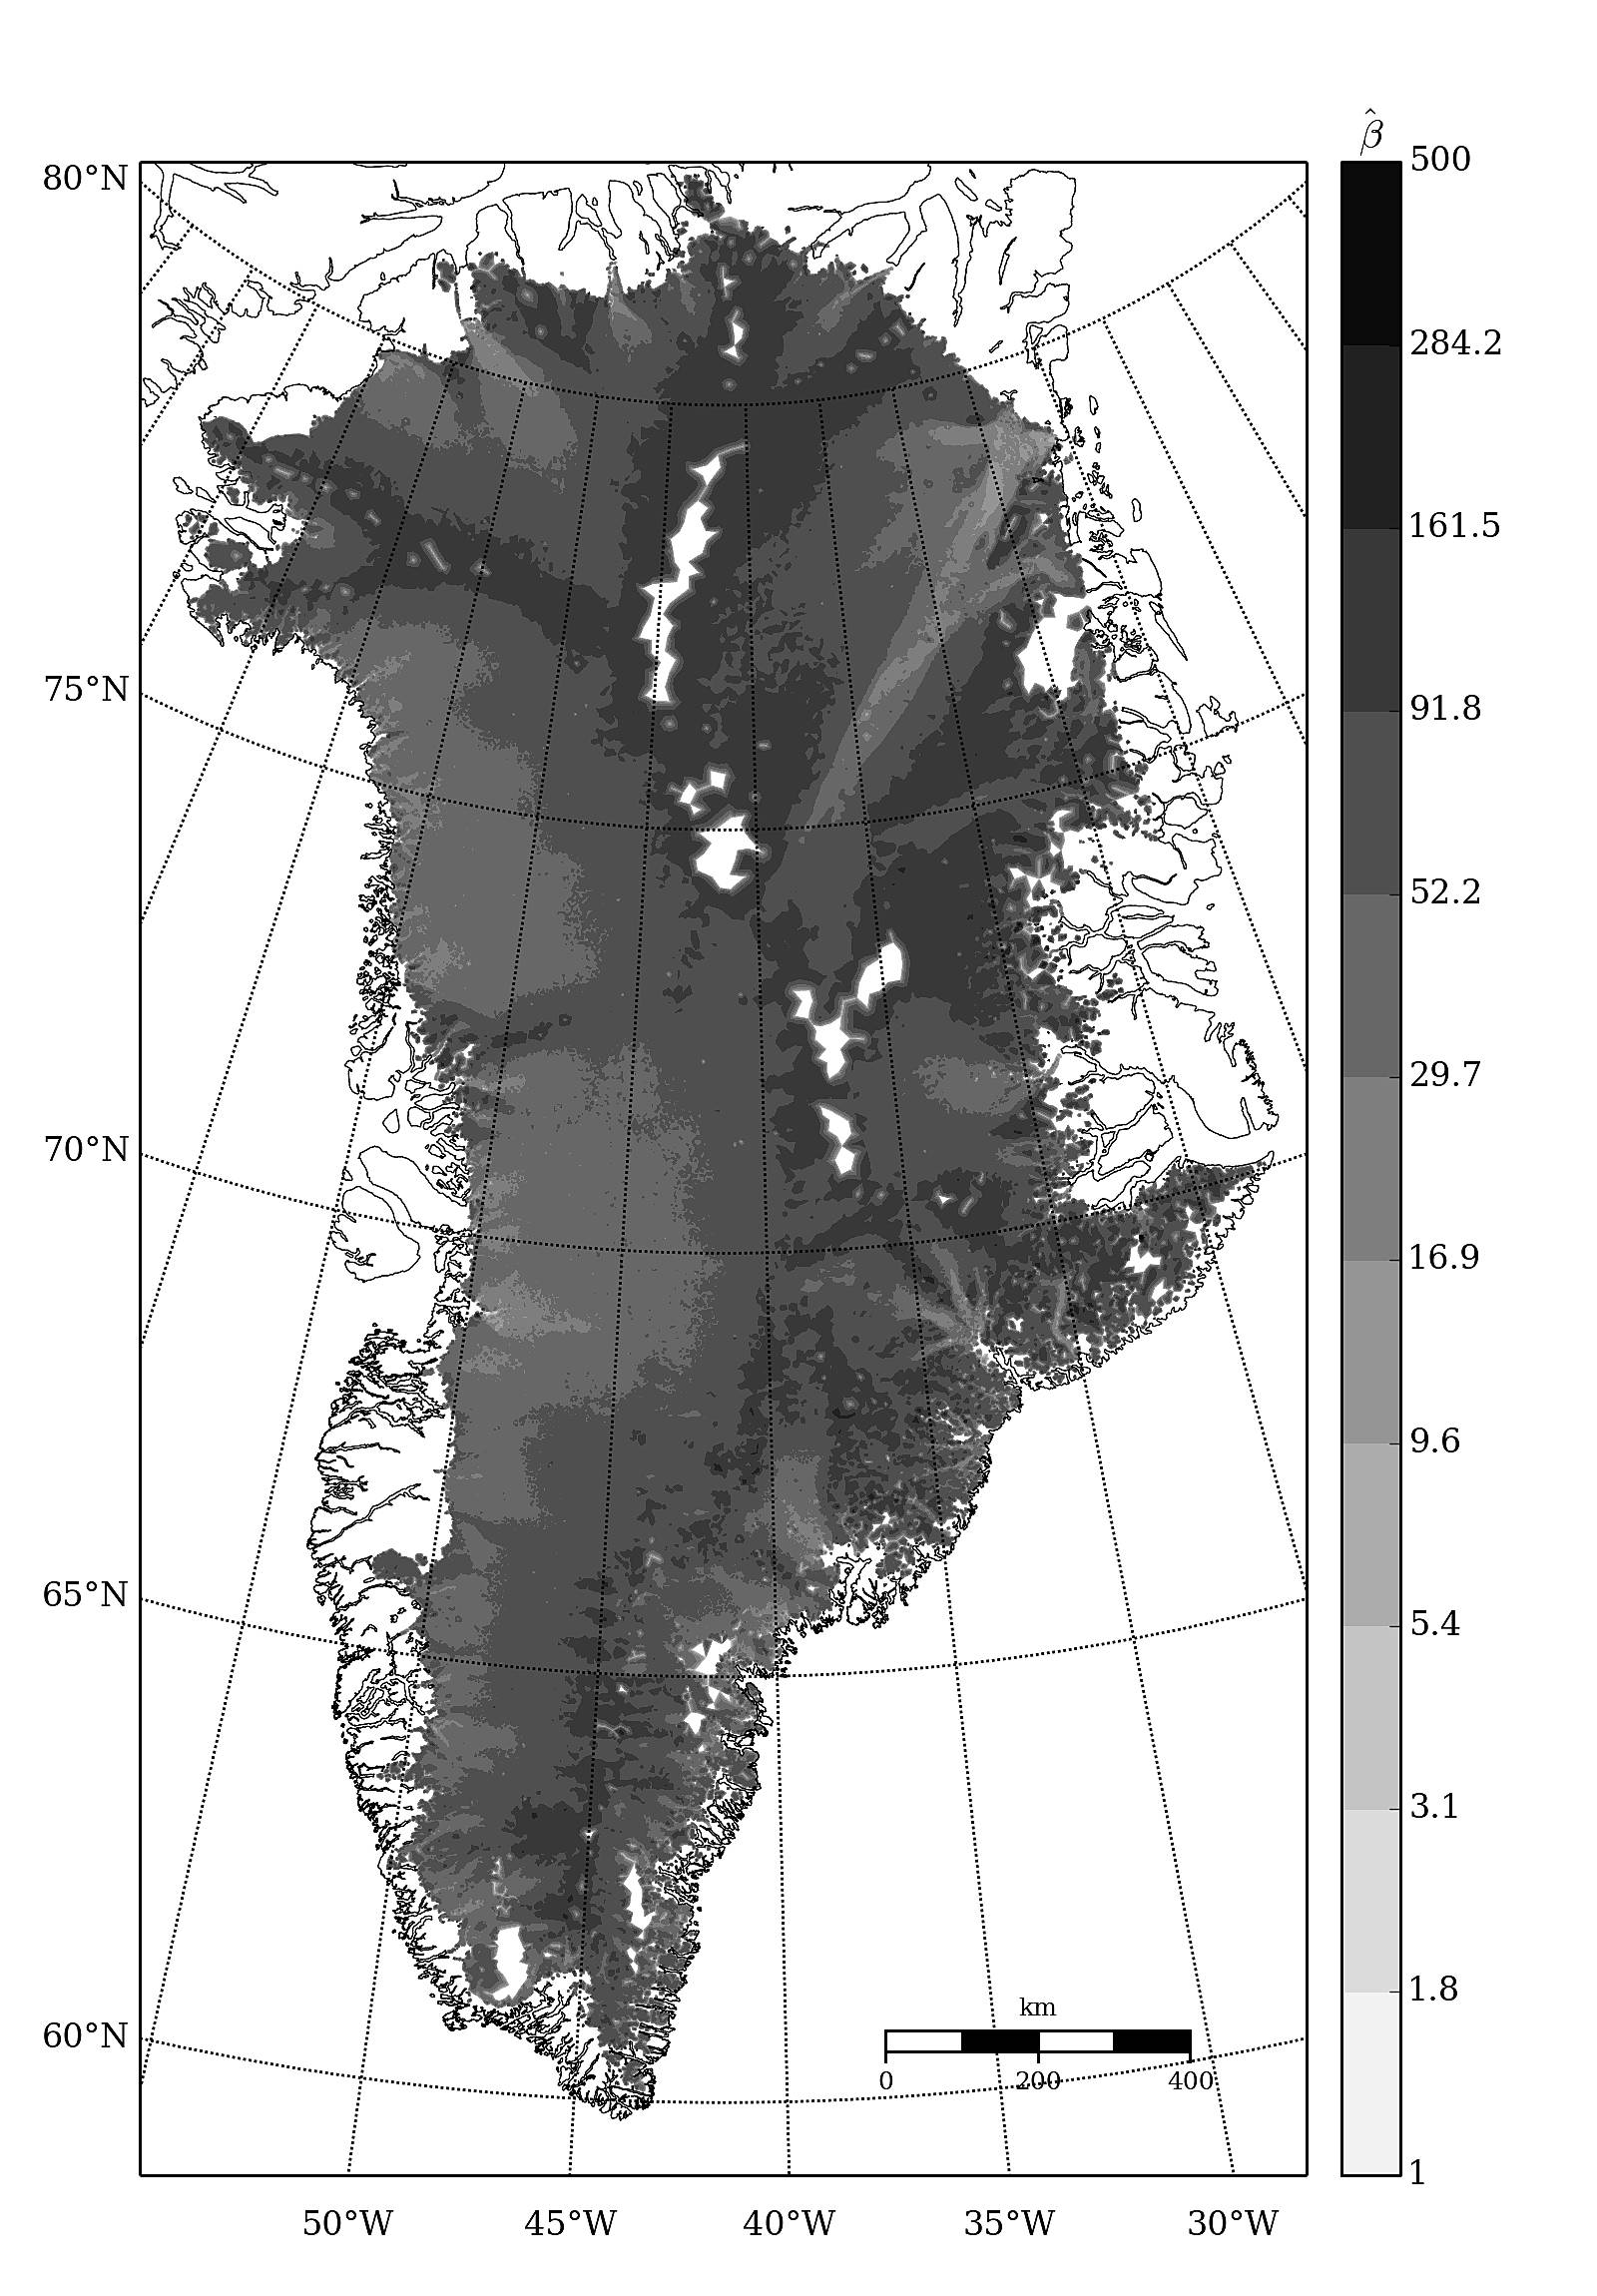
\includegraphics[width=1.0\textwidth]{images/greenland/stats/GLM_beta_no_driving_stress.jpg}
  \end{minipage}
  \quad
  \begin{minipage}[b]{0.47\linewidth}
    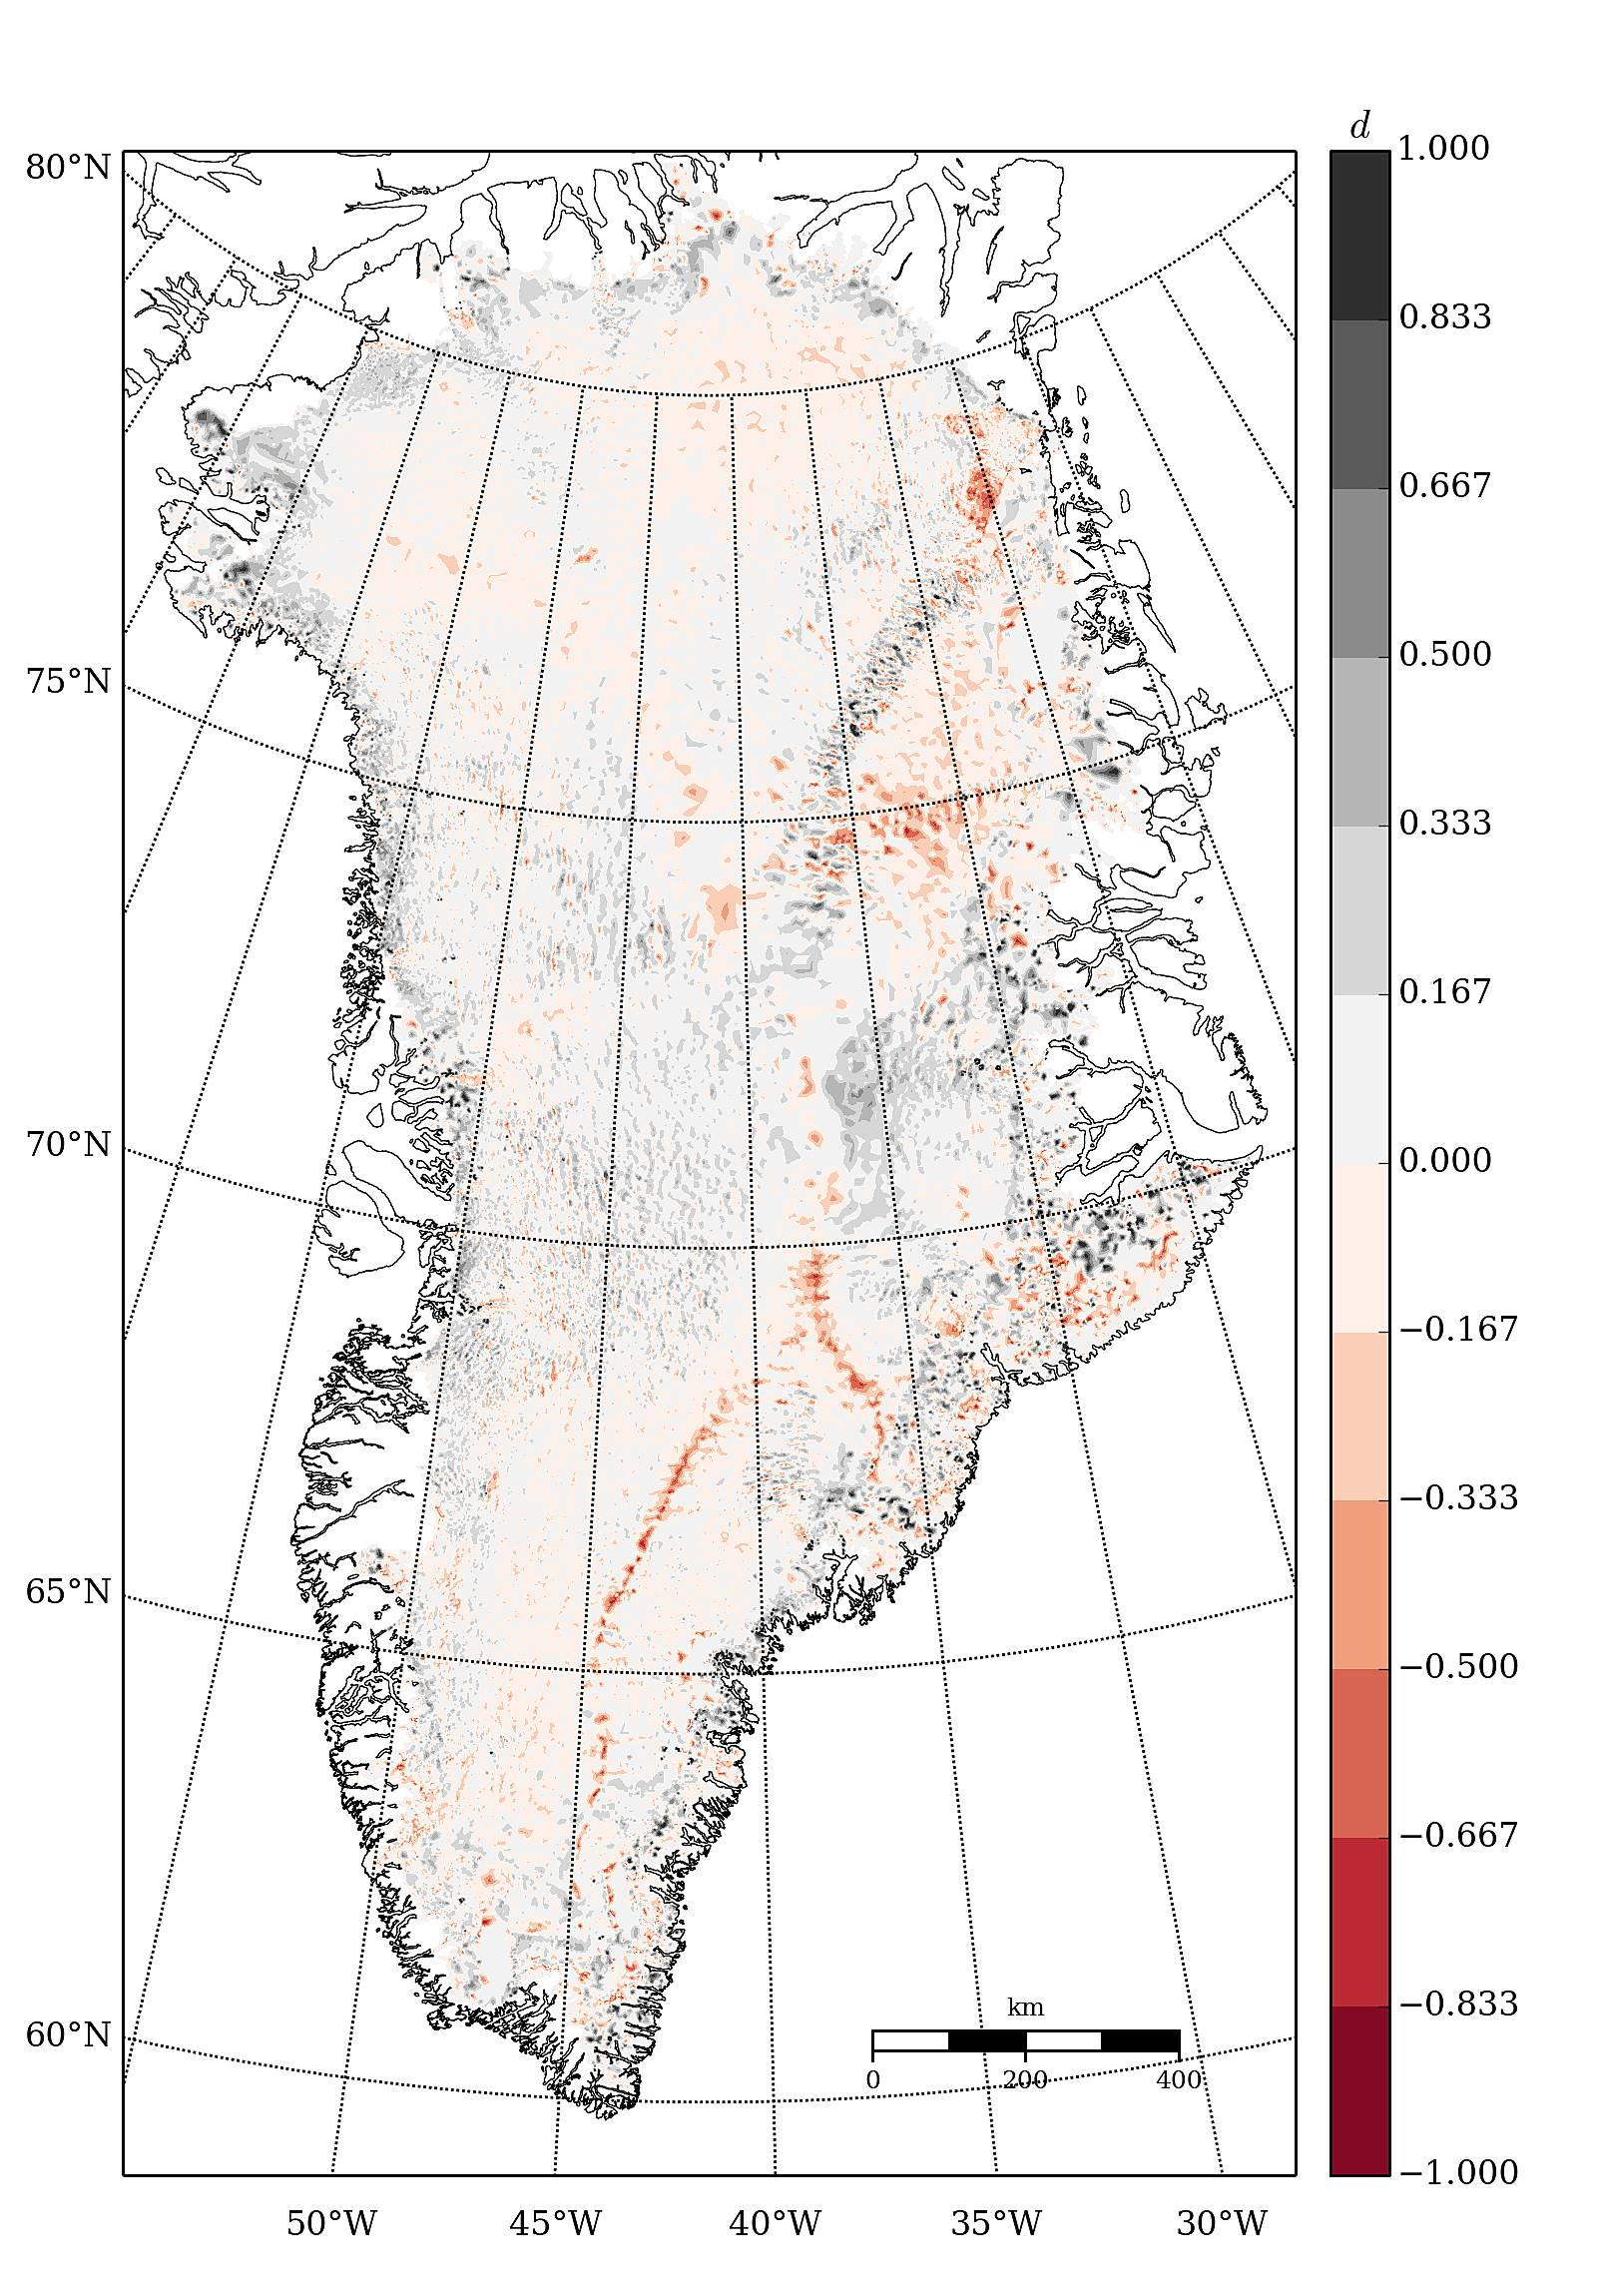
\includegraphics[width=1.0\textwidth]{images/greenland/stats/GLM_resid_no_driving_stress.jpg}
  \end{minipage}
  \begin{minipage}[b]{0.99\linewidth}
    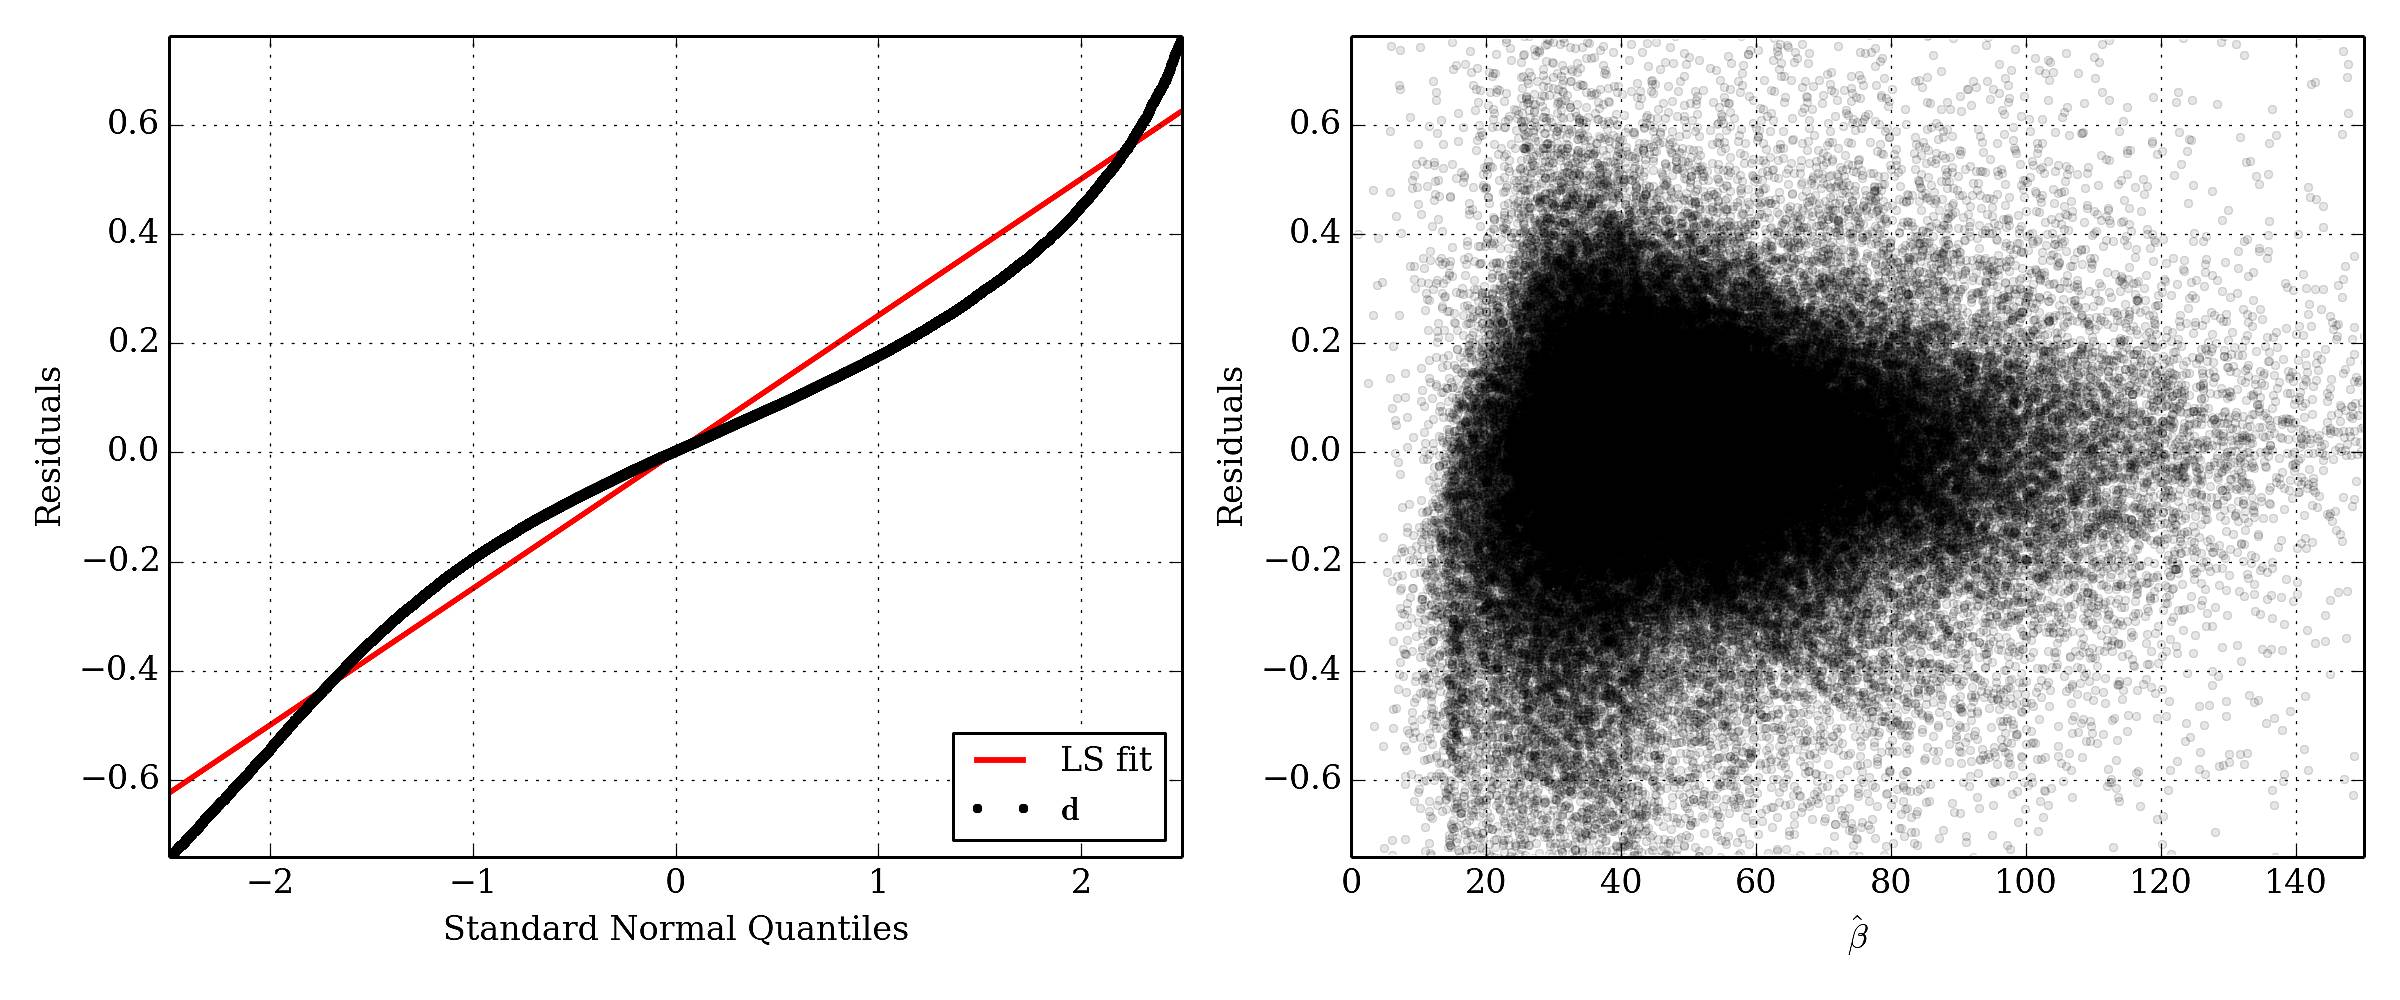
\includegraphics[width=1.0\textwidth]{images/greenland/stats/GLM_resid-NQ_no_driving_stress.jpg}
  \end{minipage}
  \caption[]{GLM model fit $\bm{\hat{\beta}}$ and residual $\mathbf{d}$, excluding $\tau_{dn}$ and $\tau_{dt}$ from $\mat{X}$.}
\end{figure}

\begin{figure}
  \centering
  \begin{minipage}[b]{0.47\linewidth}
    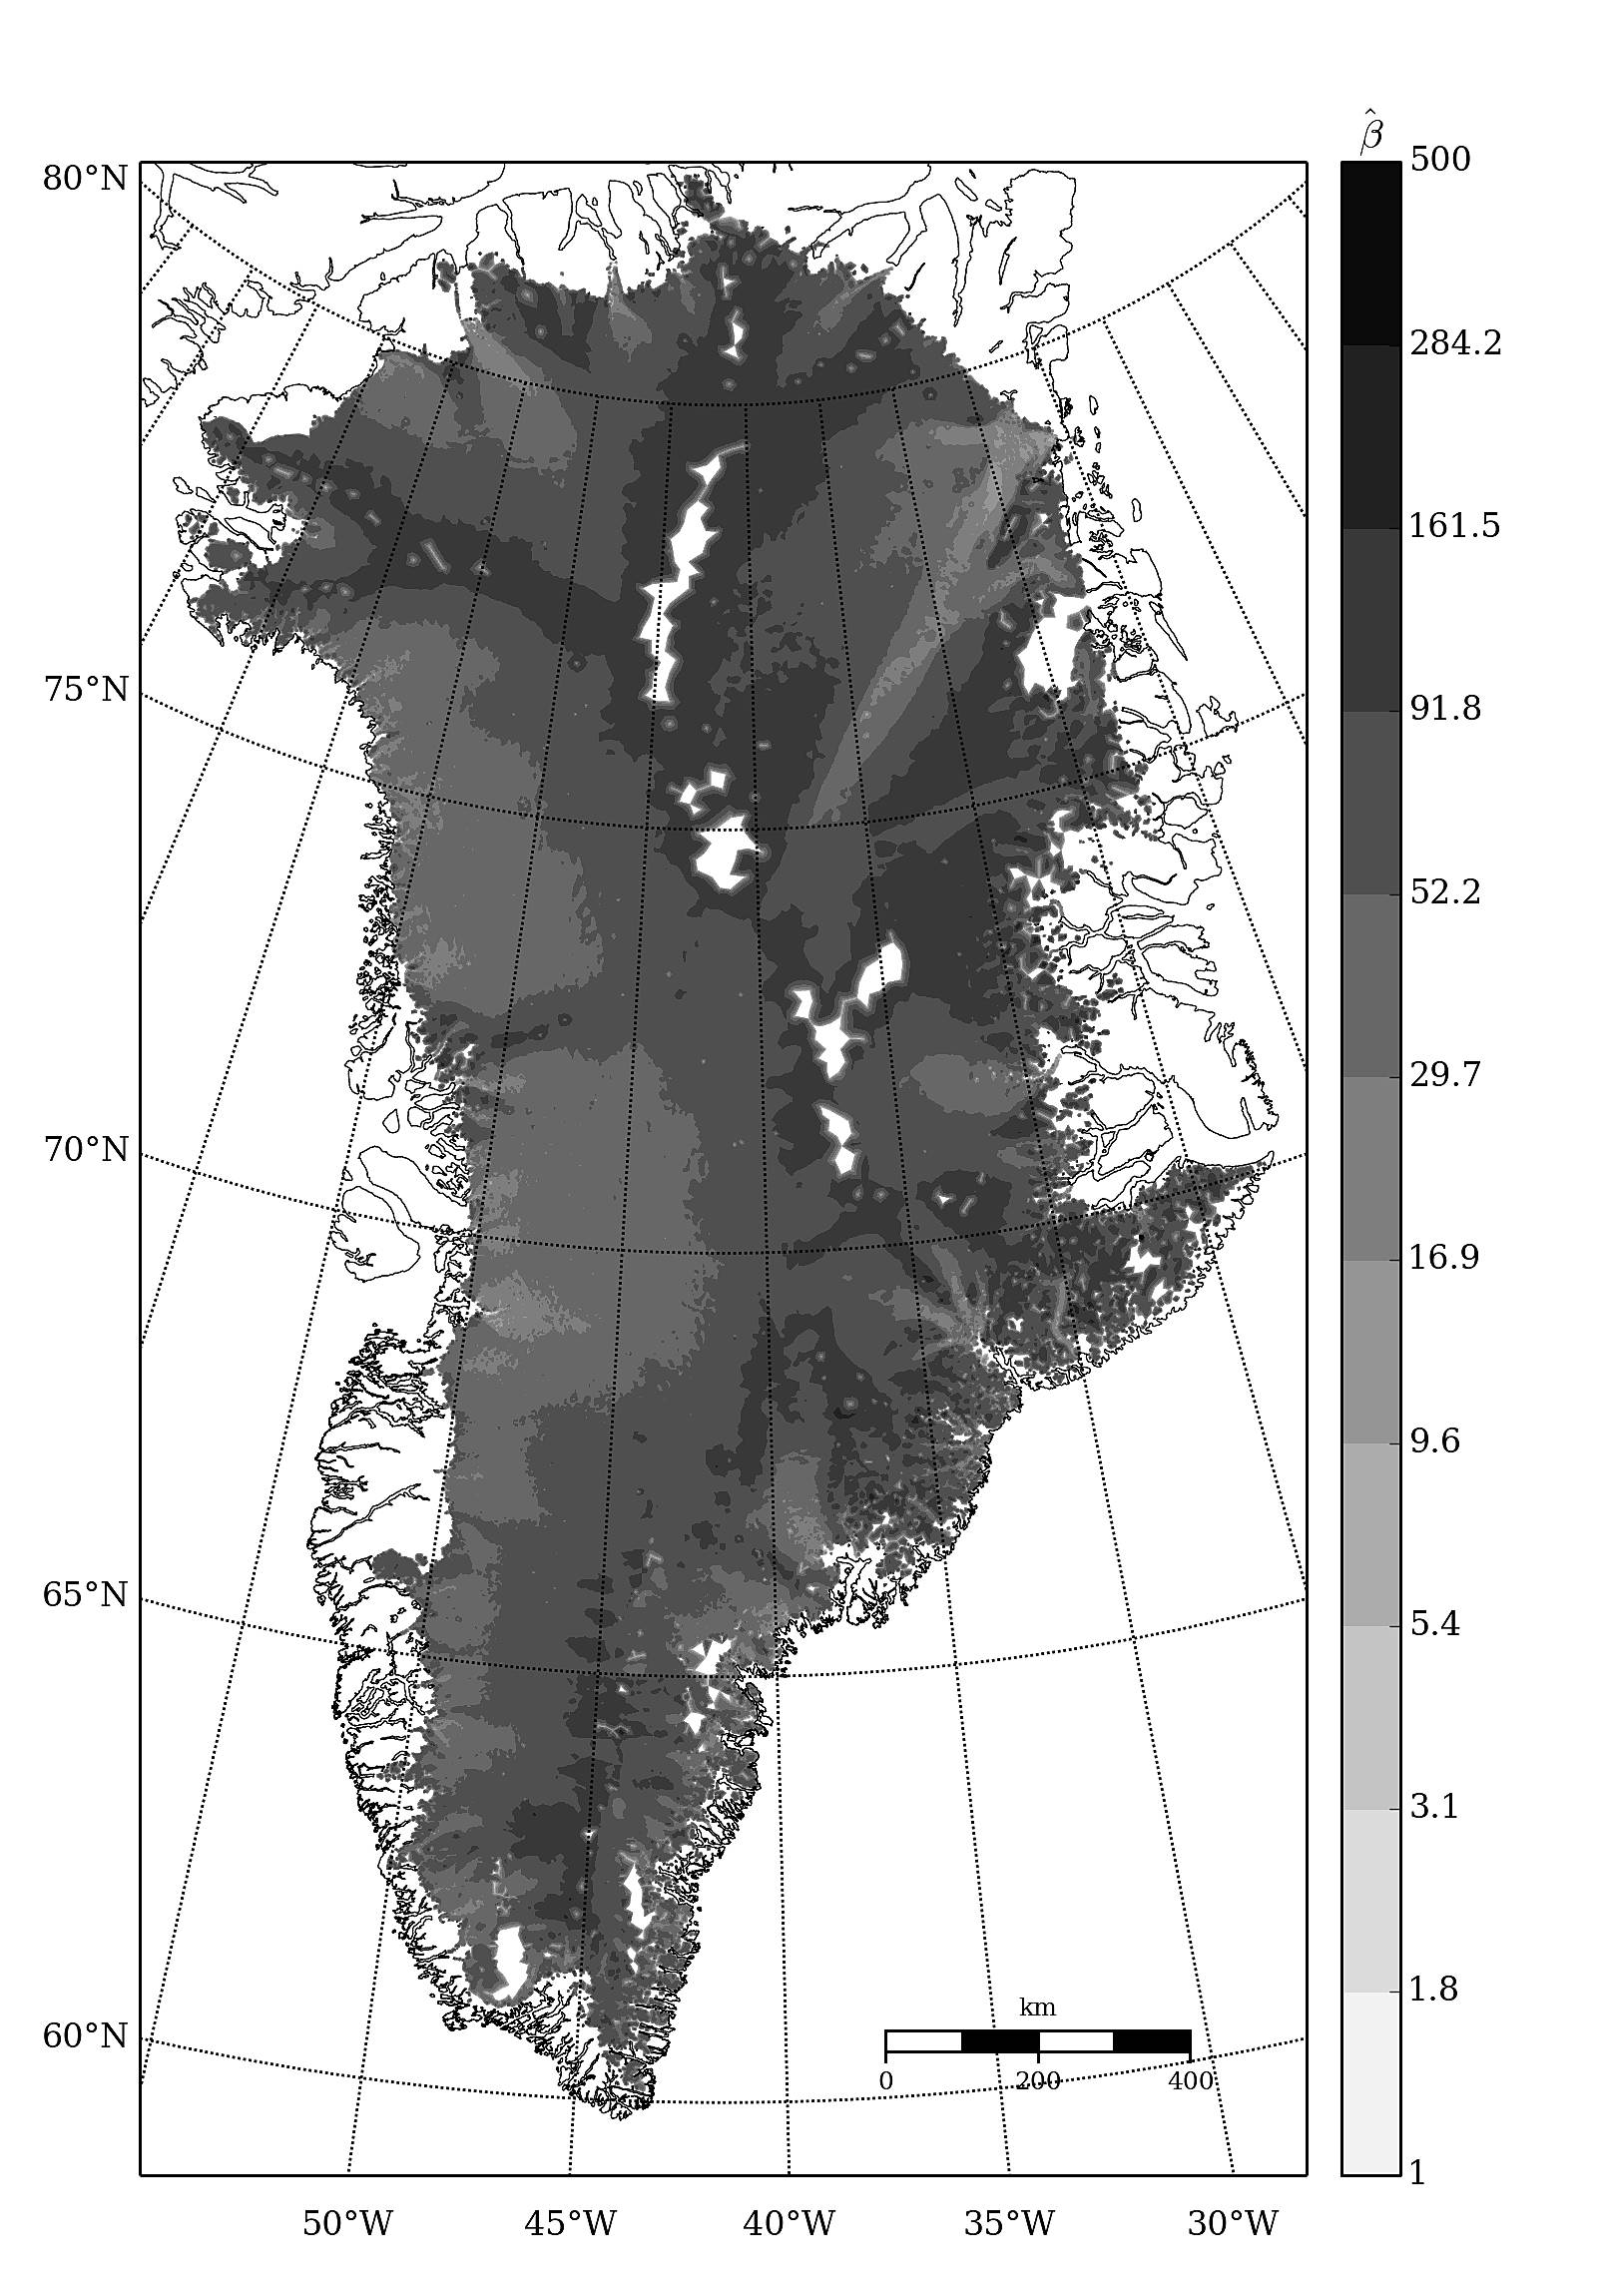
\includegraphics[width=1.0\textwidth]{images/greenland/stats/GLM_beta_no_stress.jpg}
  \end{minipage}
  \quad
  \begin{minipage}[b]{0.47\linewidth}
    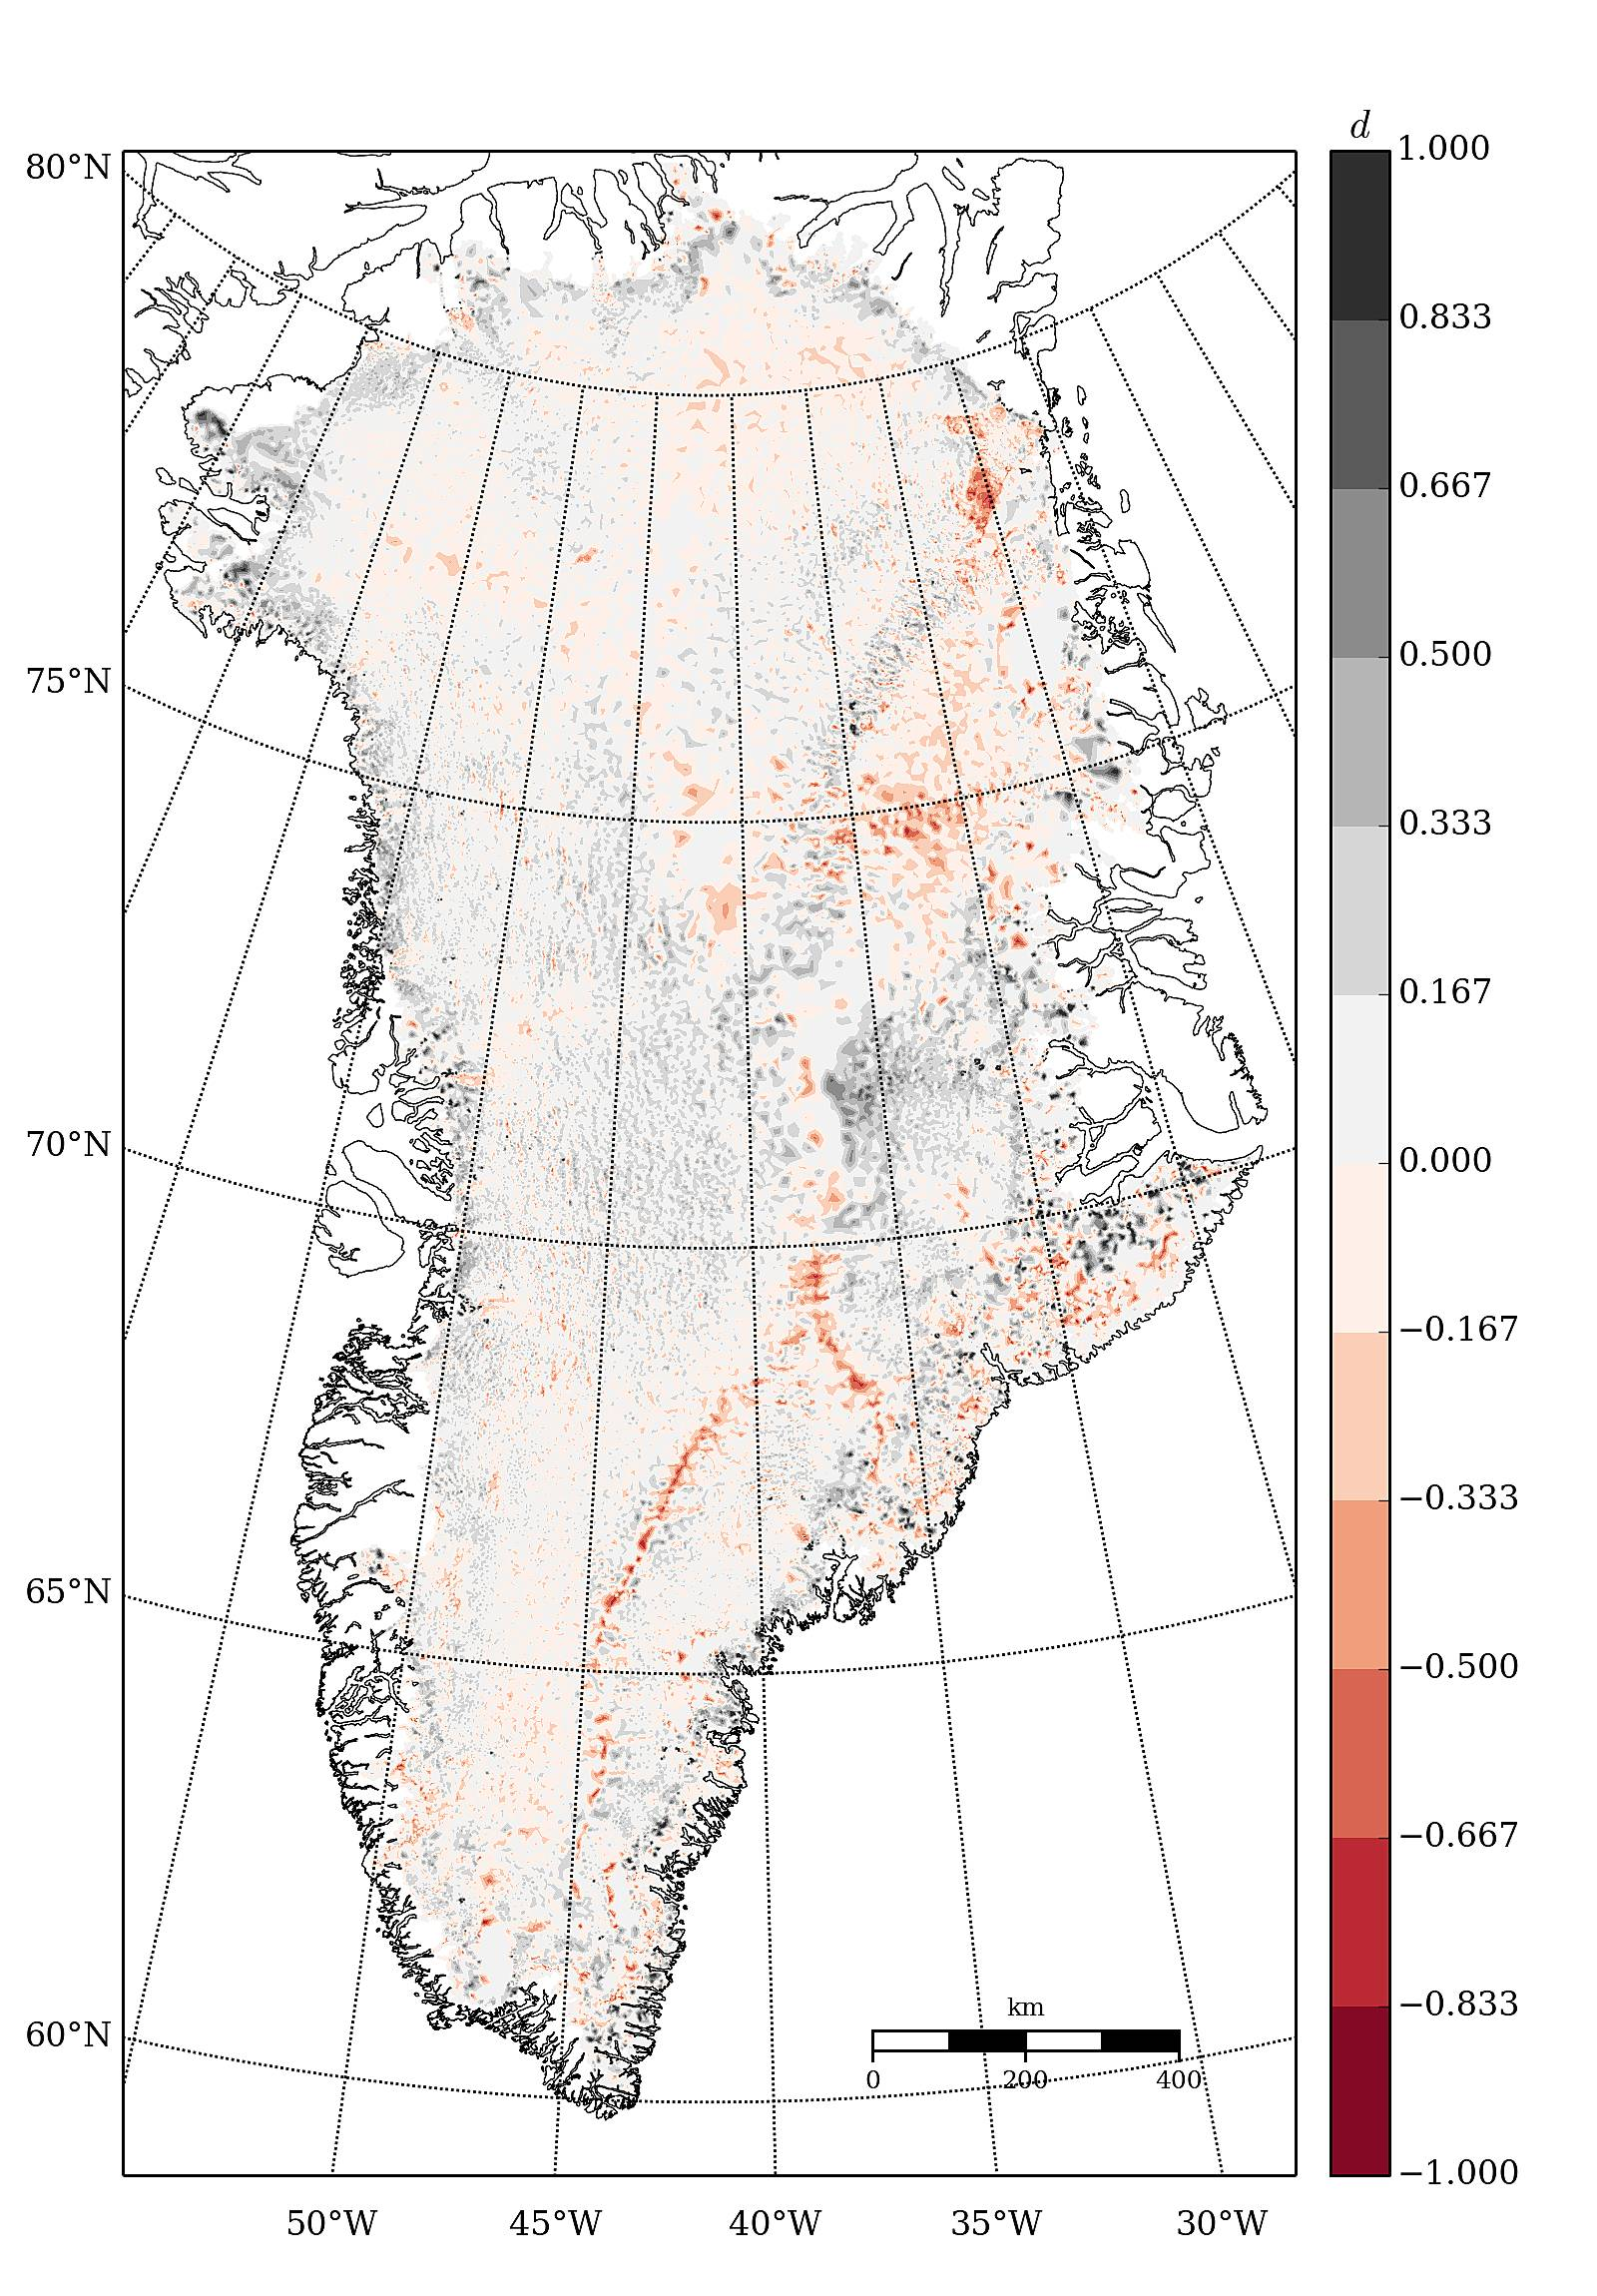
\includegraphics[width=1.0\textwidth]{images/greenland/stats/GLM_resid_no_stress.jpg}
  \end{minipage}
  \begin{minipage}[b]{0.99\linewidth}
    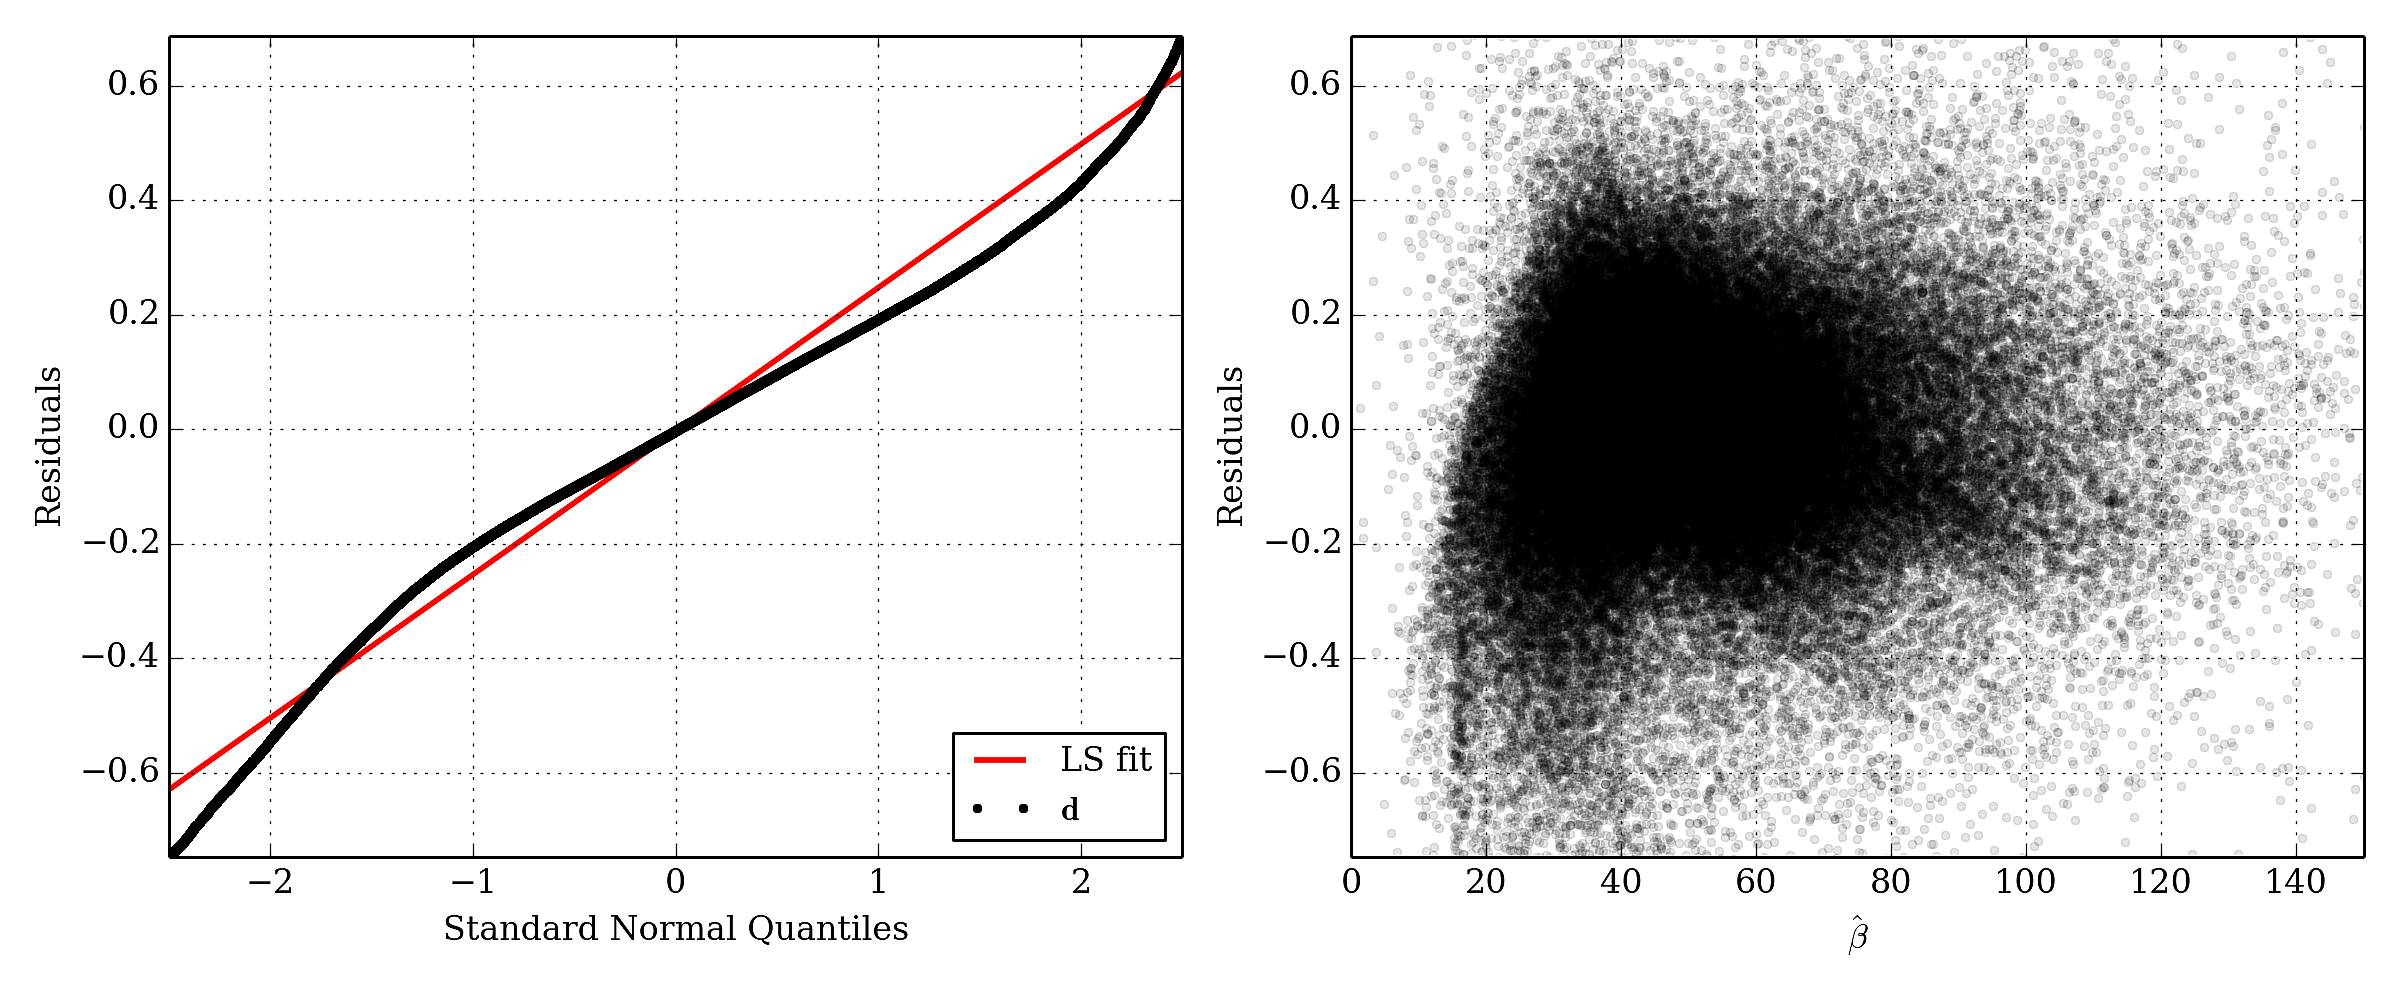
\includegraphics[width=1.0\textwidth]{images/greenland/stats/GLM_resid-NQ_no_stress.jpg}
  \end{minipage}
  \caption[]{GLM model fit $\bm{\hat{\beta}}$ and residual $\mathbf{d}$, excluding $\tau_{nn}$, $\tau_{nt}$, $\tau_{tn}$, $\tau_{tt}$, $\tau_{dn}$, and $\tau_{dt}$ from $\mat{X}$.}
\end{figure}

\begin{figure}
  \centering
  \begin{minipage}[b]{0.47\linewidth}
    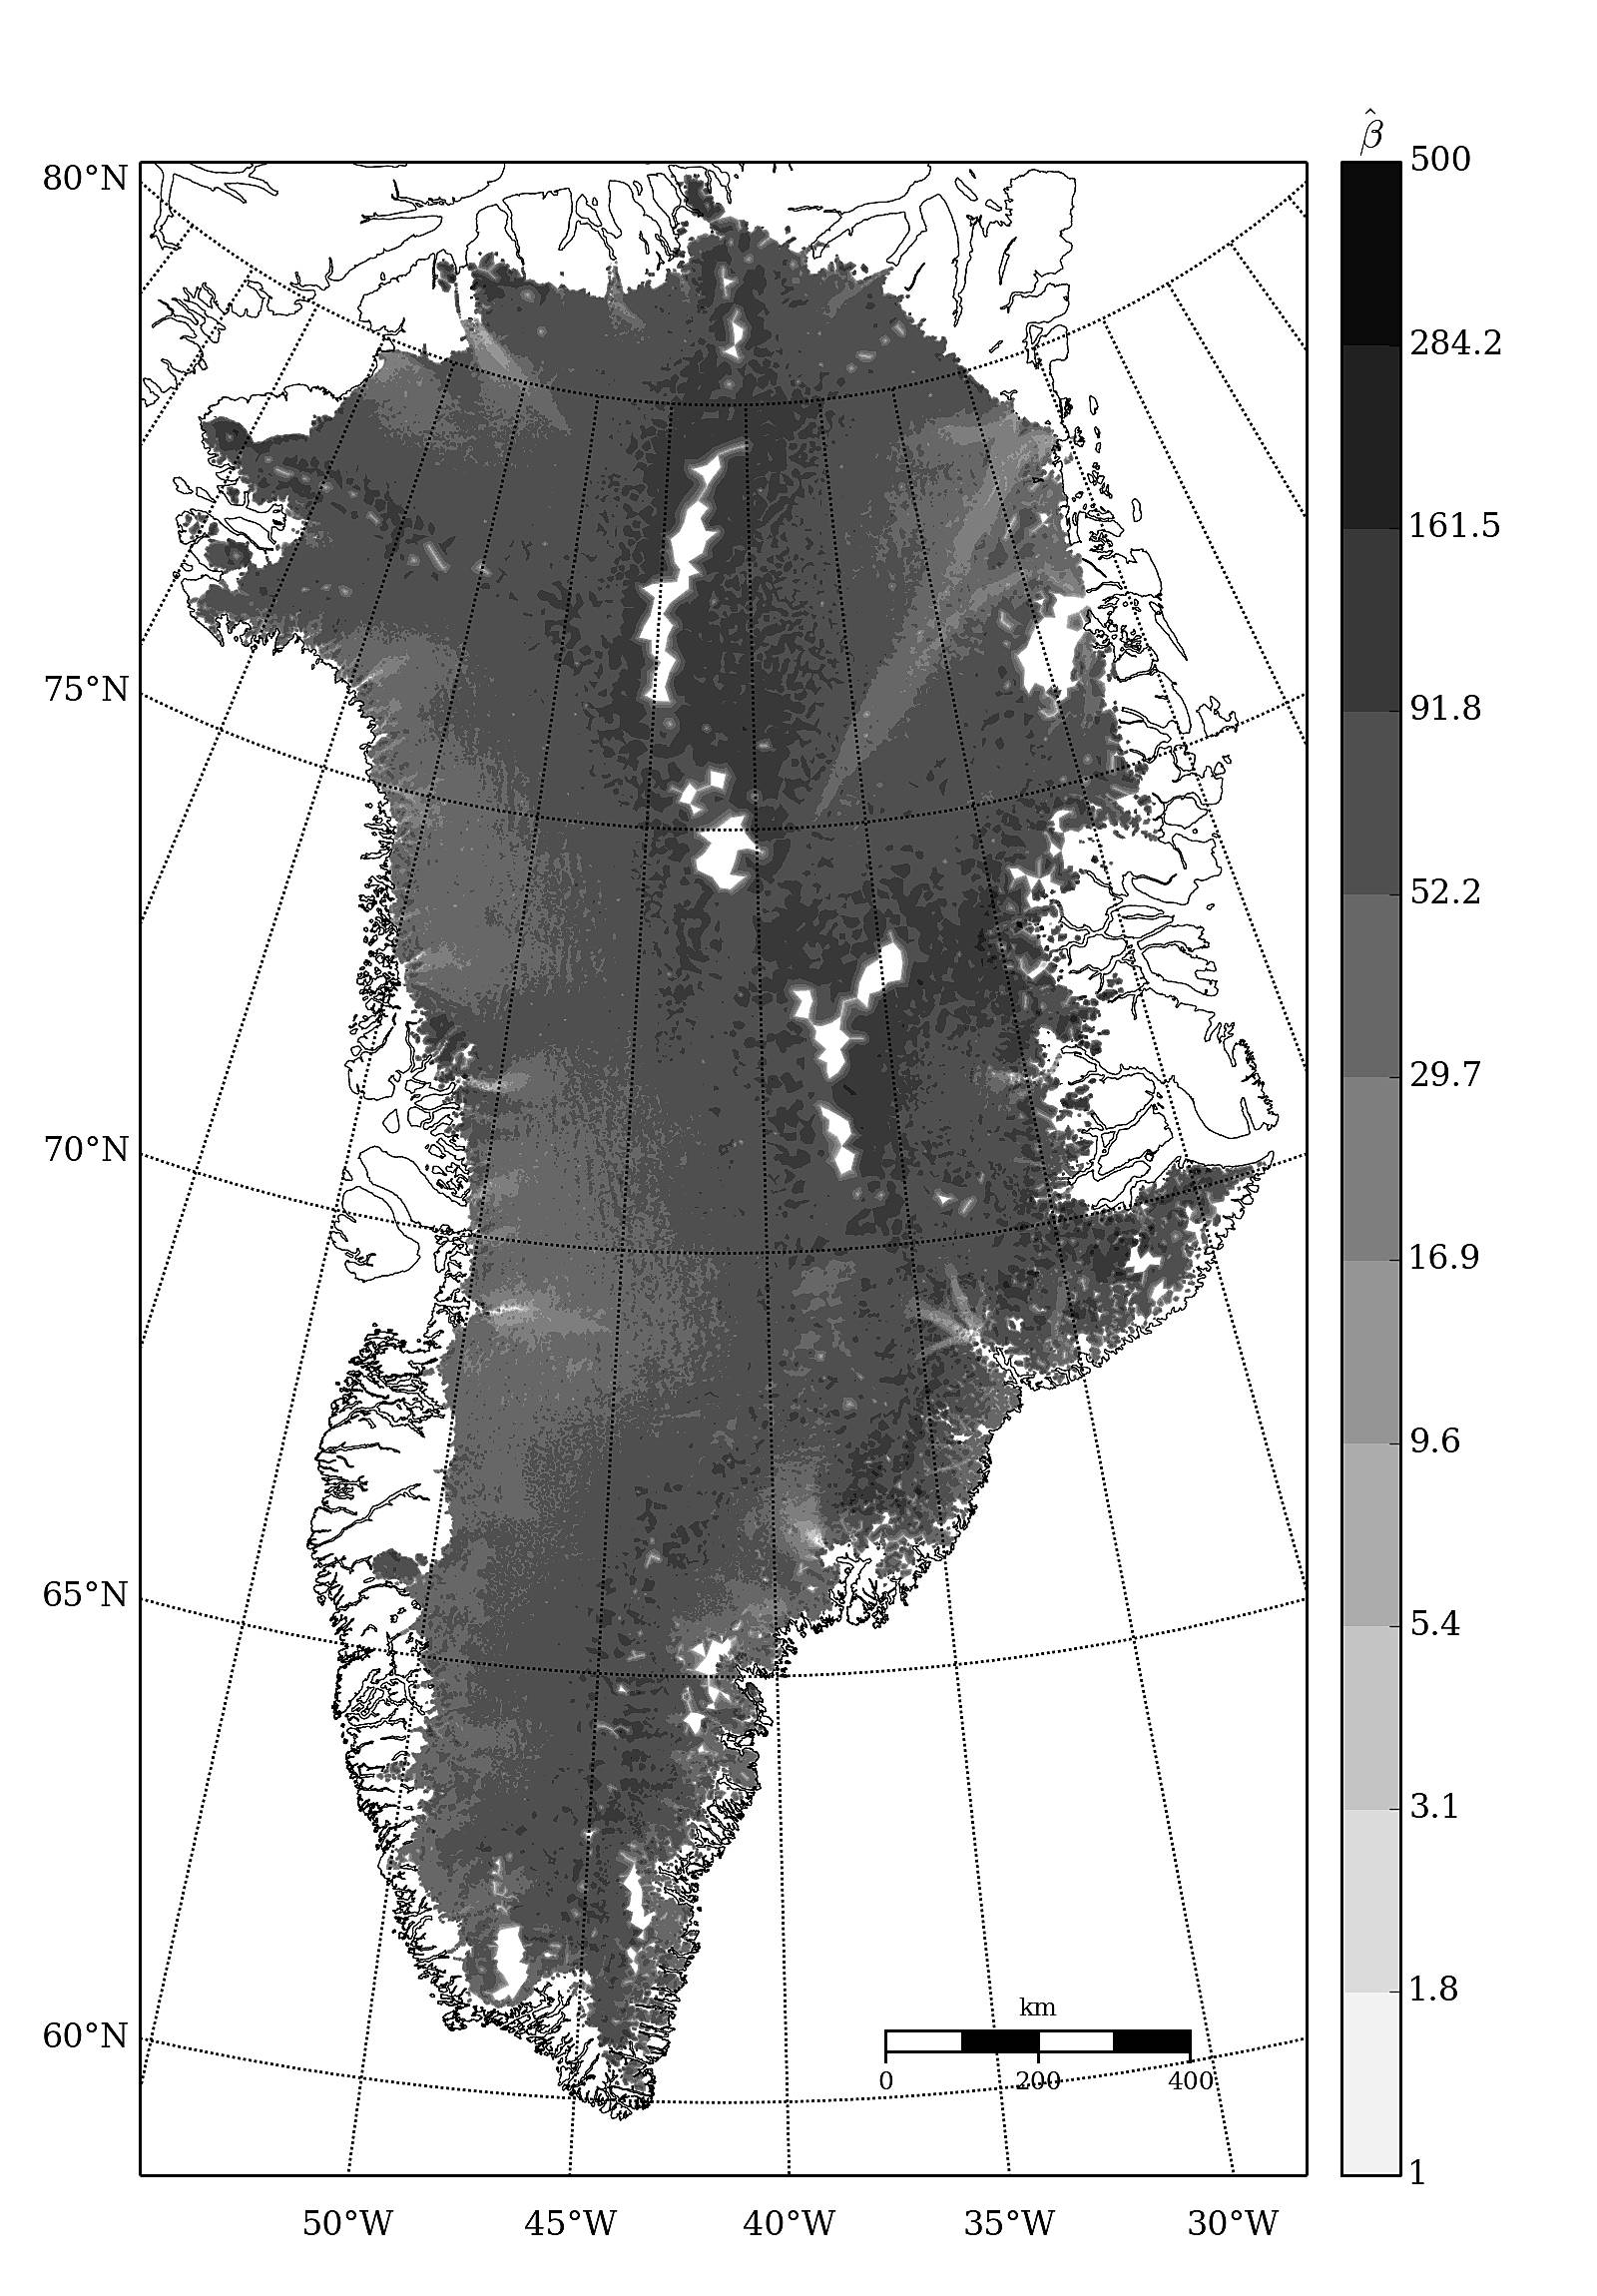
\includegraphics[width=1.0\textwidth]{images/greenland/stats/GLM_beta_no_U.jpg}
  \end{minipage}
  \quad
  \begin{minipage}[b]{0.47\linewidth}
    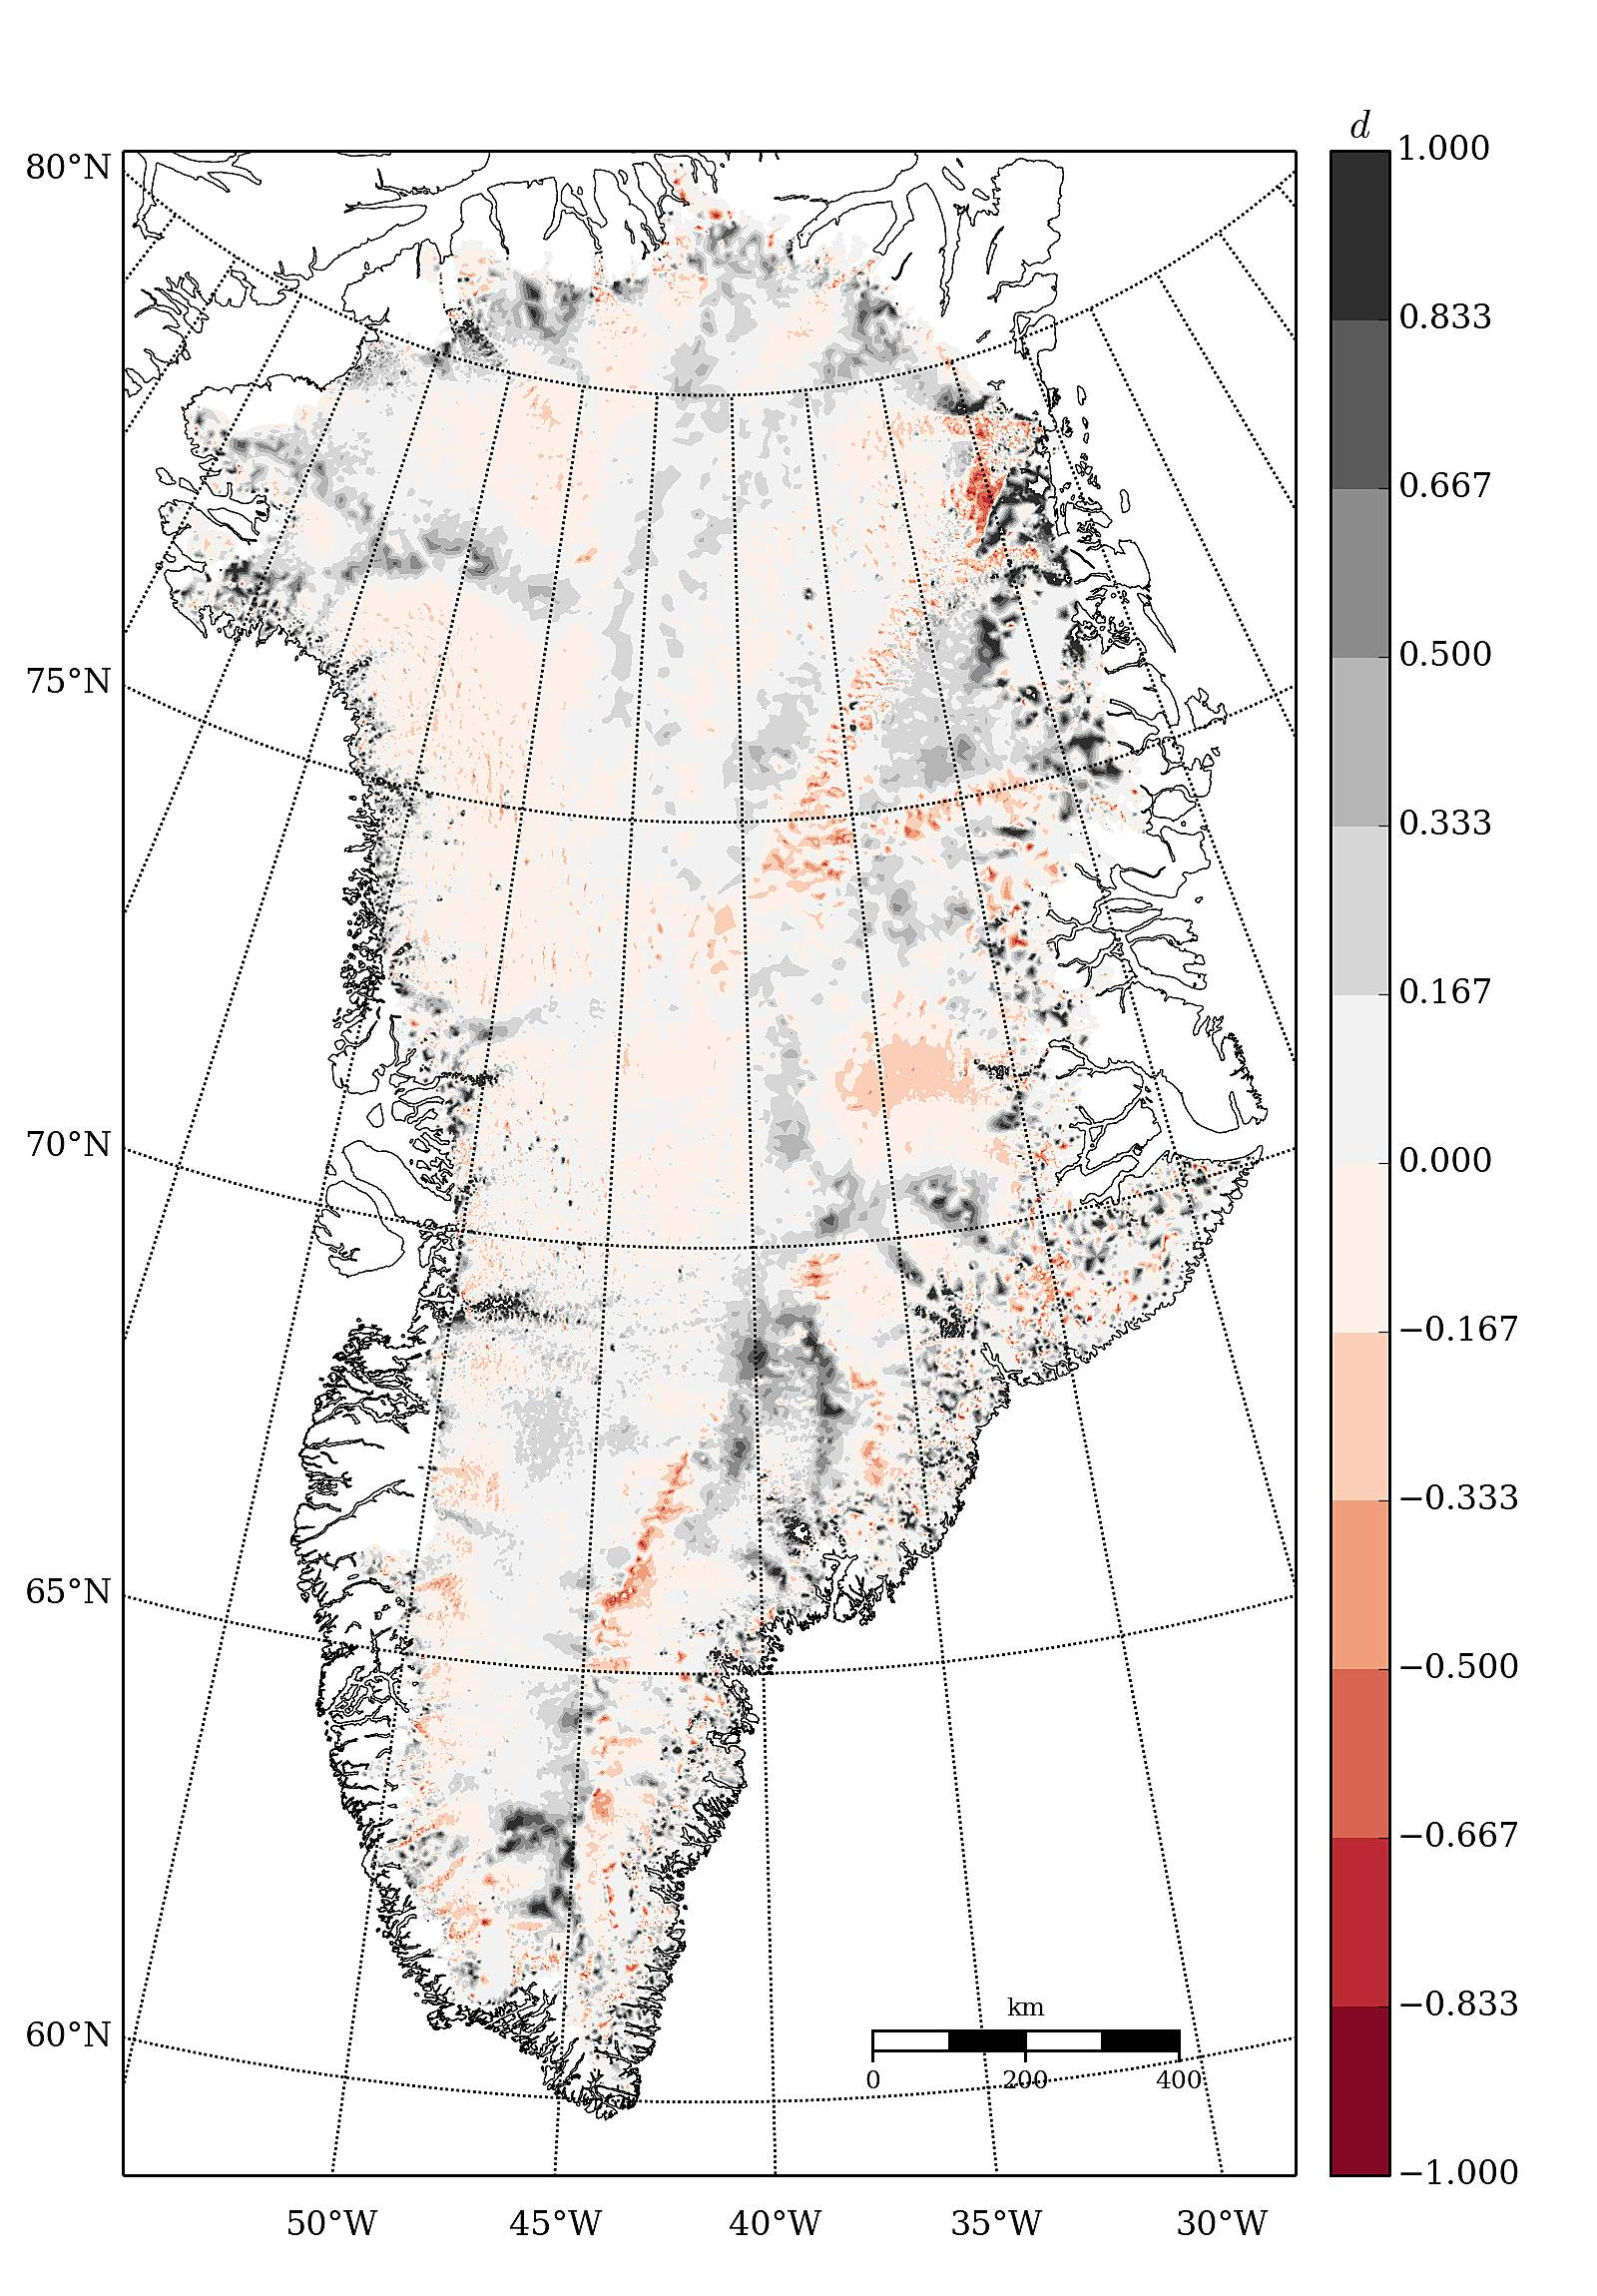
\includegraphics[width=1.0\textwidth]{images/greenland/stats/GLM_resid_no_U.jpg}
  \end{minipage}
  \begin{minipage}[b]{0.99\linewidth}
    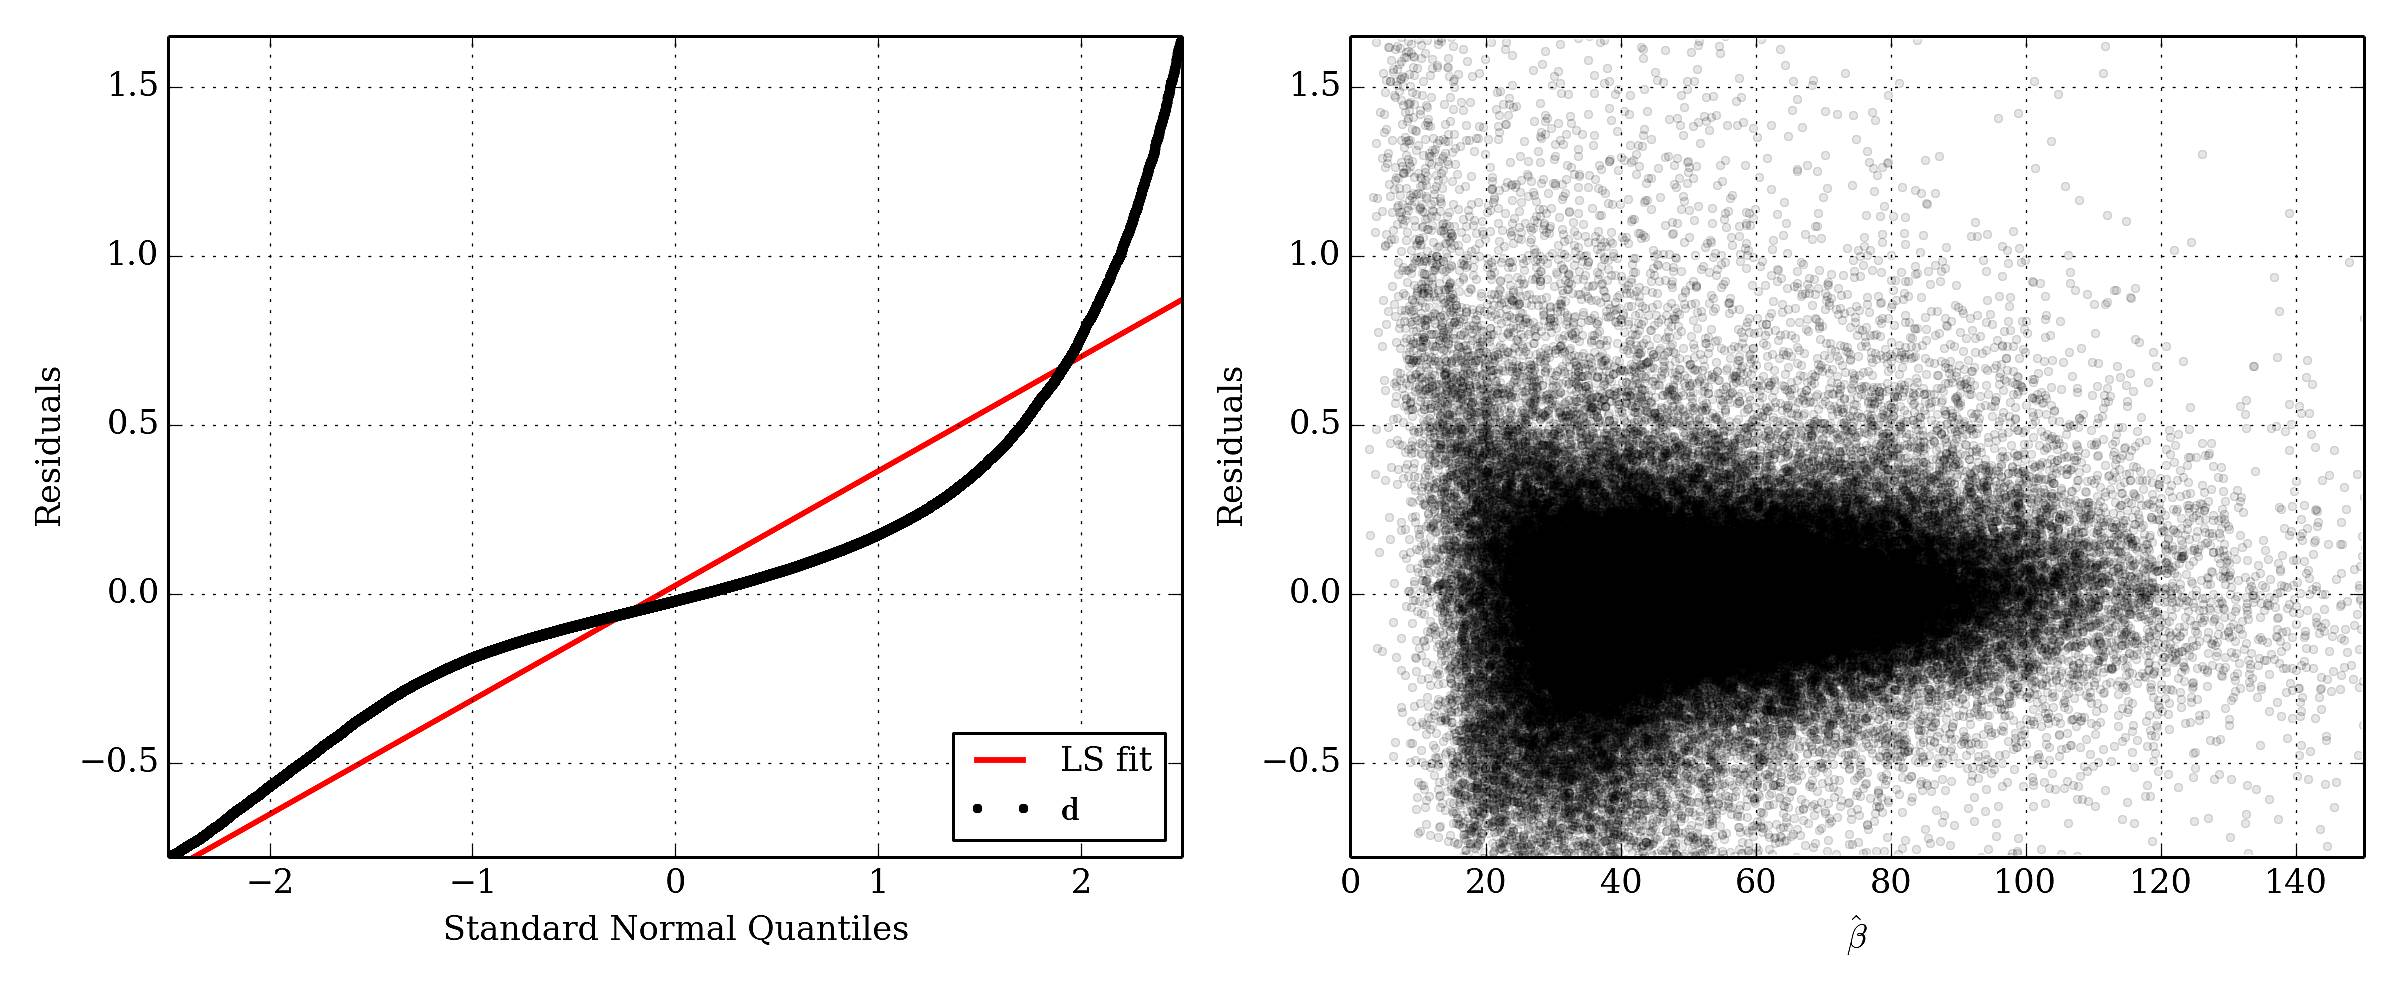
\includegraphics[width=1.0\textwidth]{images/greenland/stats/GLM_resid-NQ_no_U.jpg}
  \end{minipage}
  \caption[]{GLM model fit $\bm{\hat{\beta}}$ and residual $\mathbf{d}$, excluding $\ln\left(\Vert \mathbf{U}_B \Vert + 1\right)$ from $\mat{X}$.}
\end{figure}

\begin{figure}
  \centering
  \begin{minipage}[b]{0.47\linewidth}
    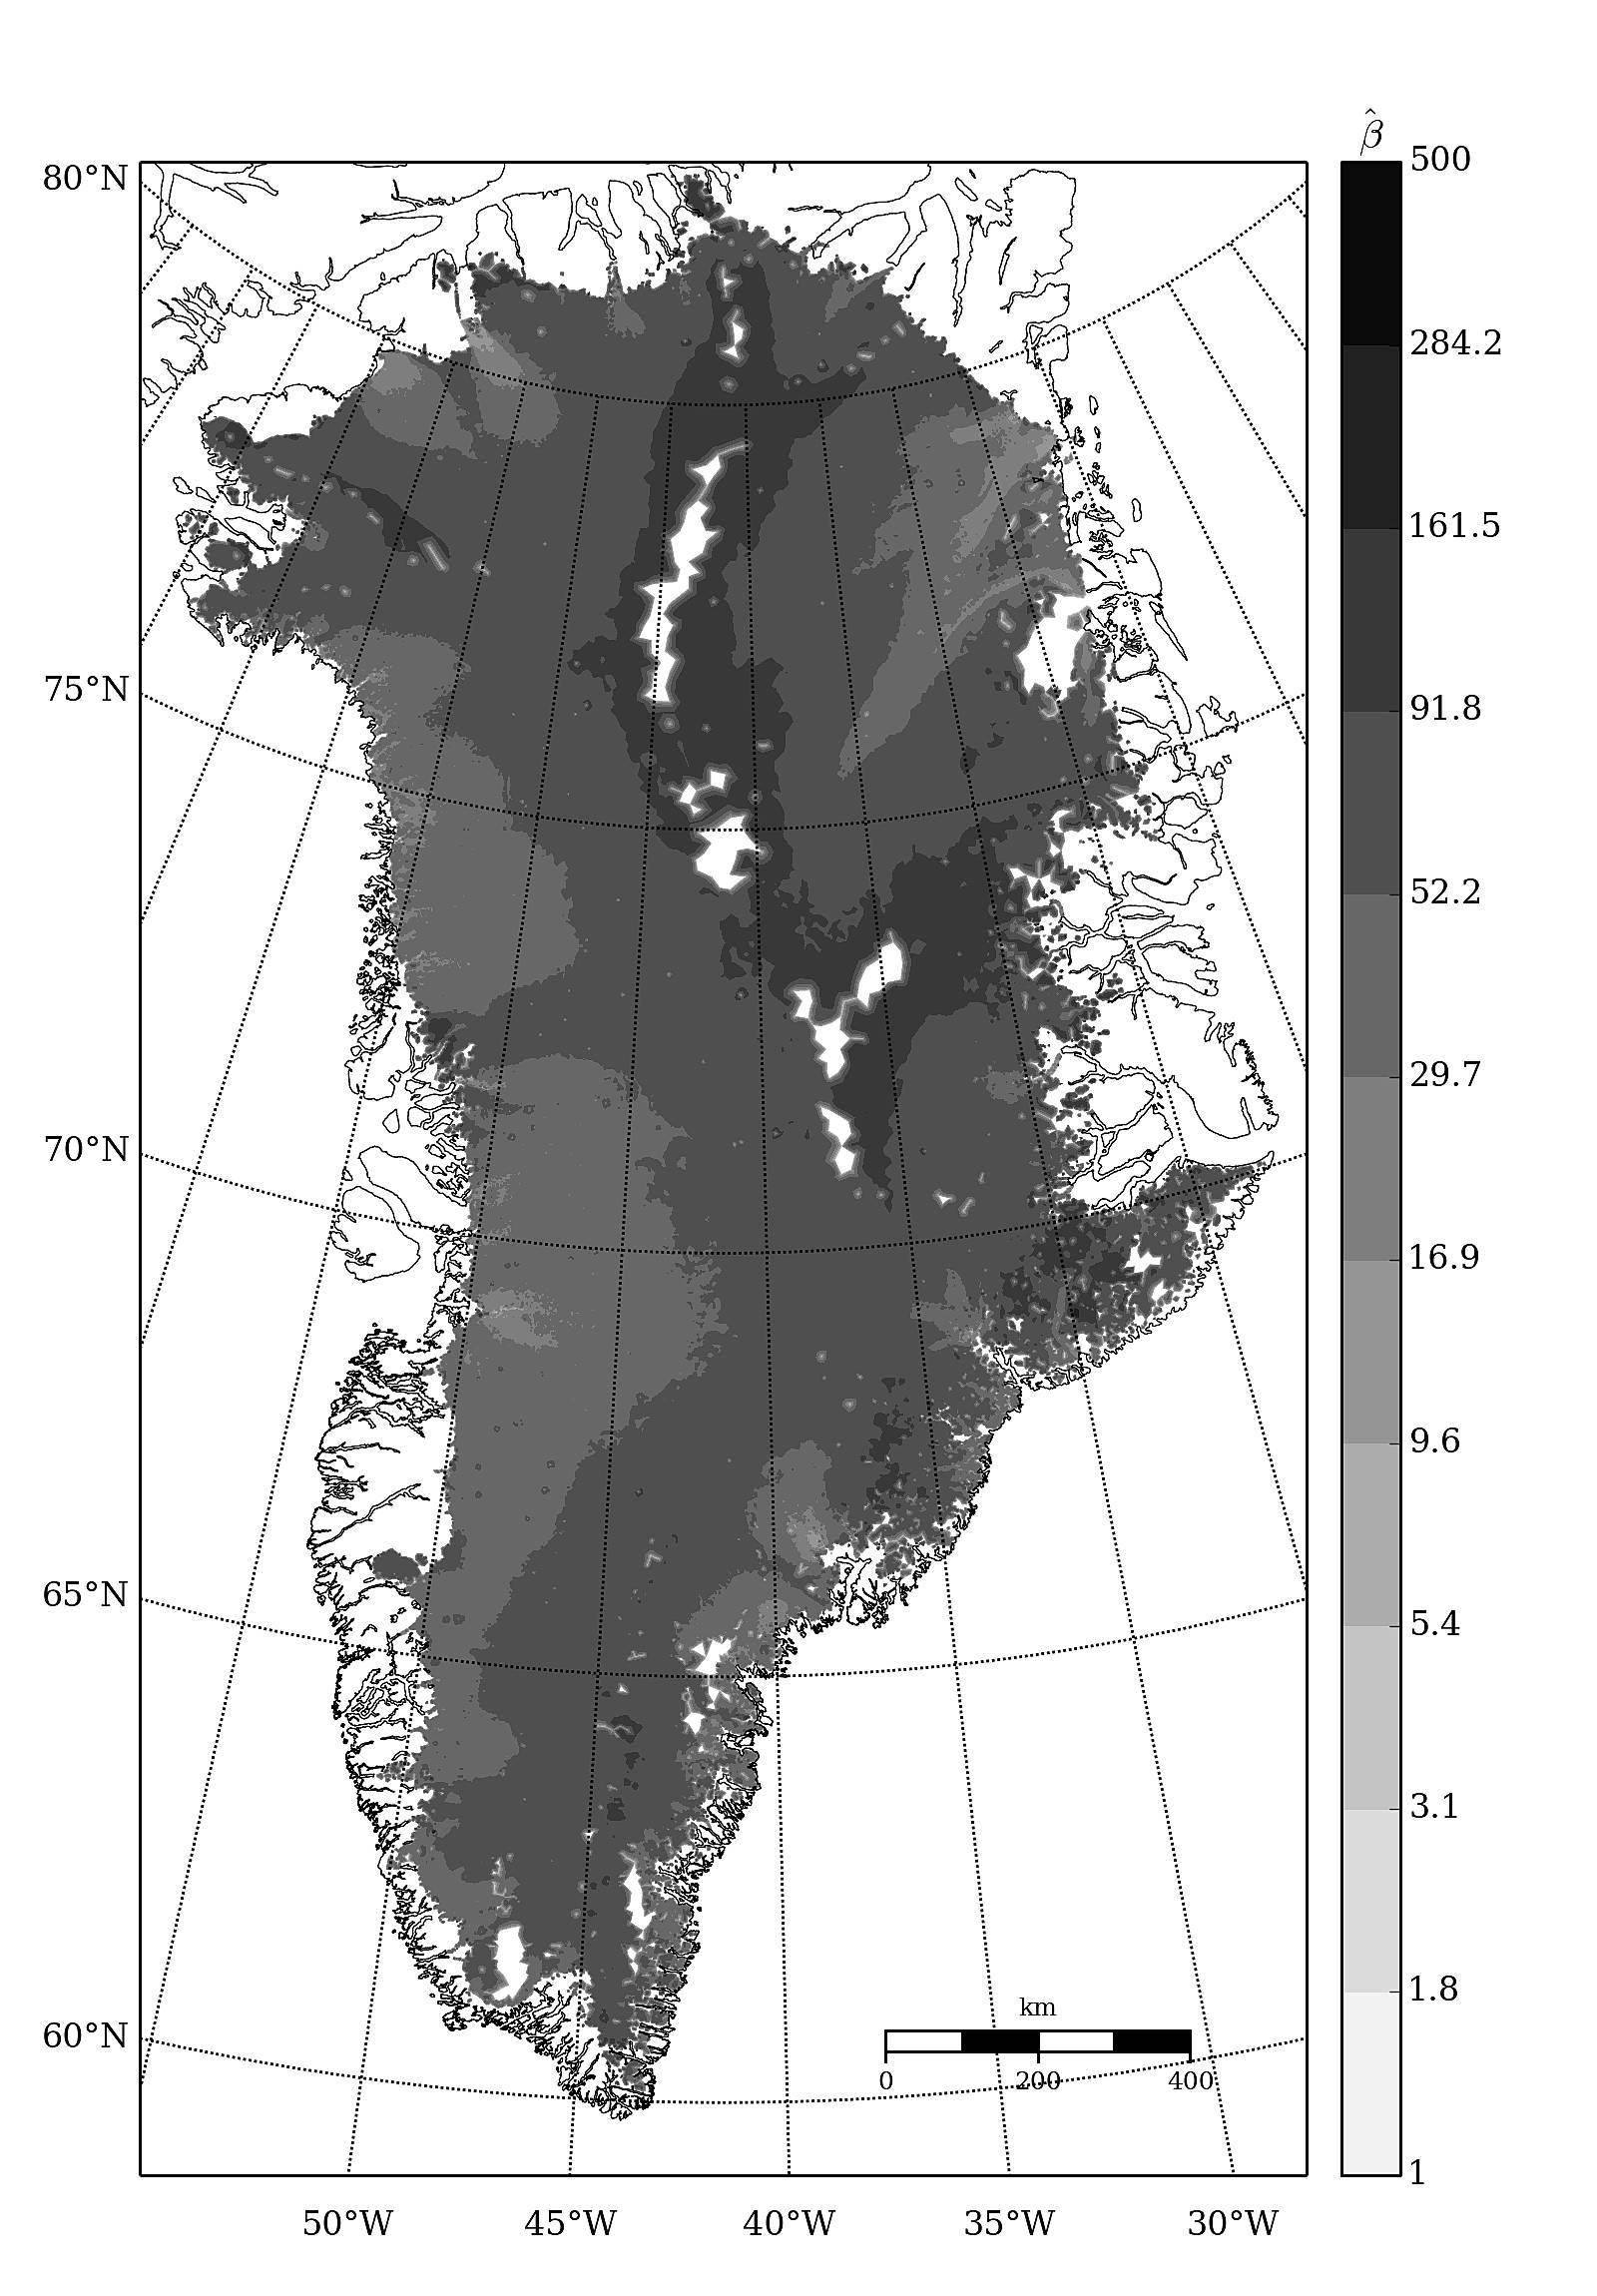
\includegraphics[width=1.0\textwidth]{images/greenland/stats/GLM_beta_no_velocity.jpg}
  \end{minipage}
  \quad
  \begin{minipage}[b]{0.47\linewidth}
    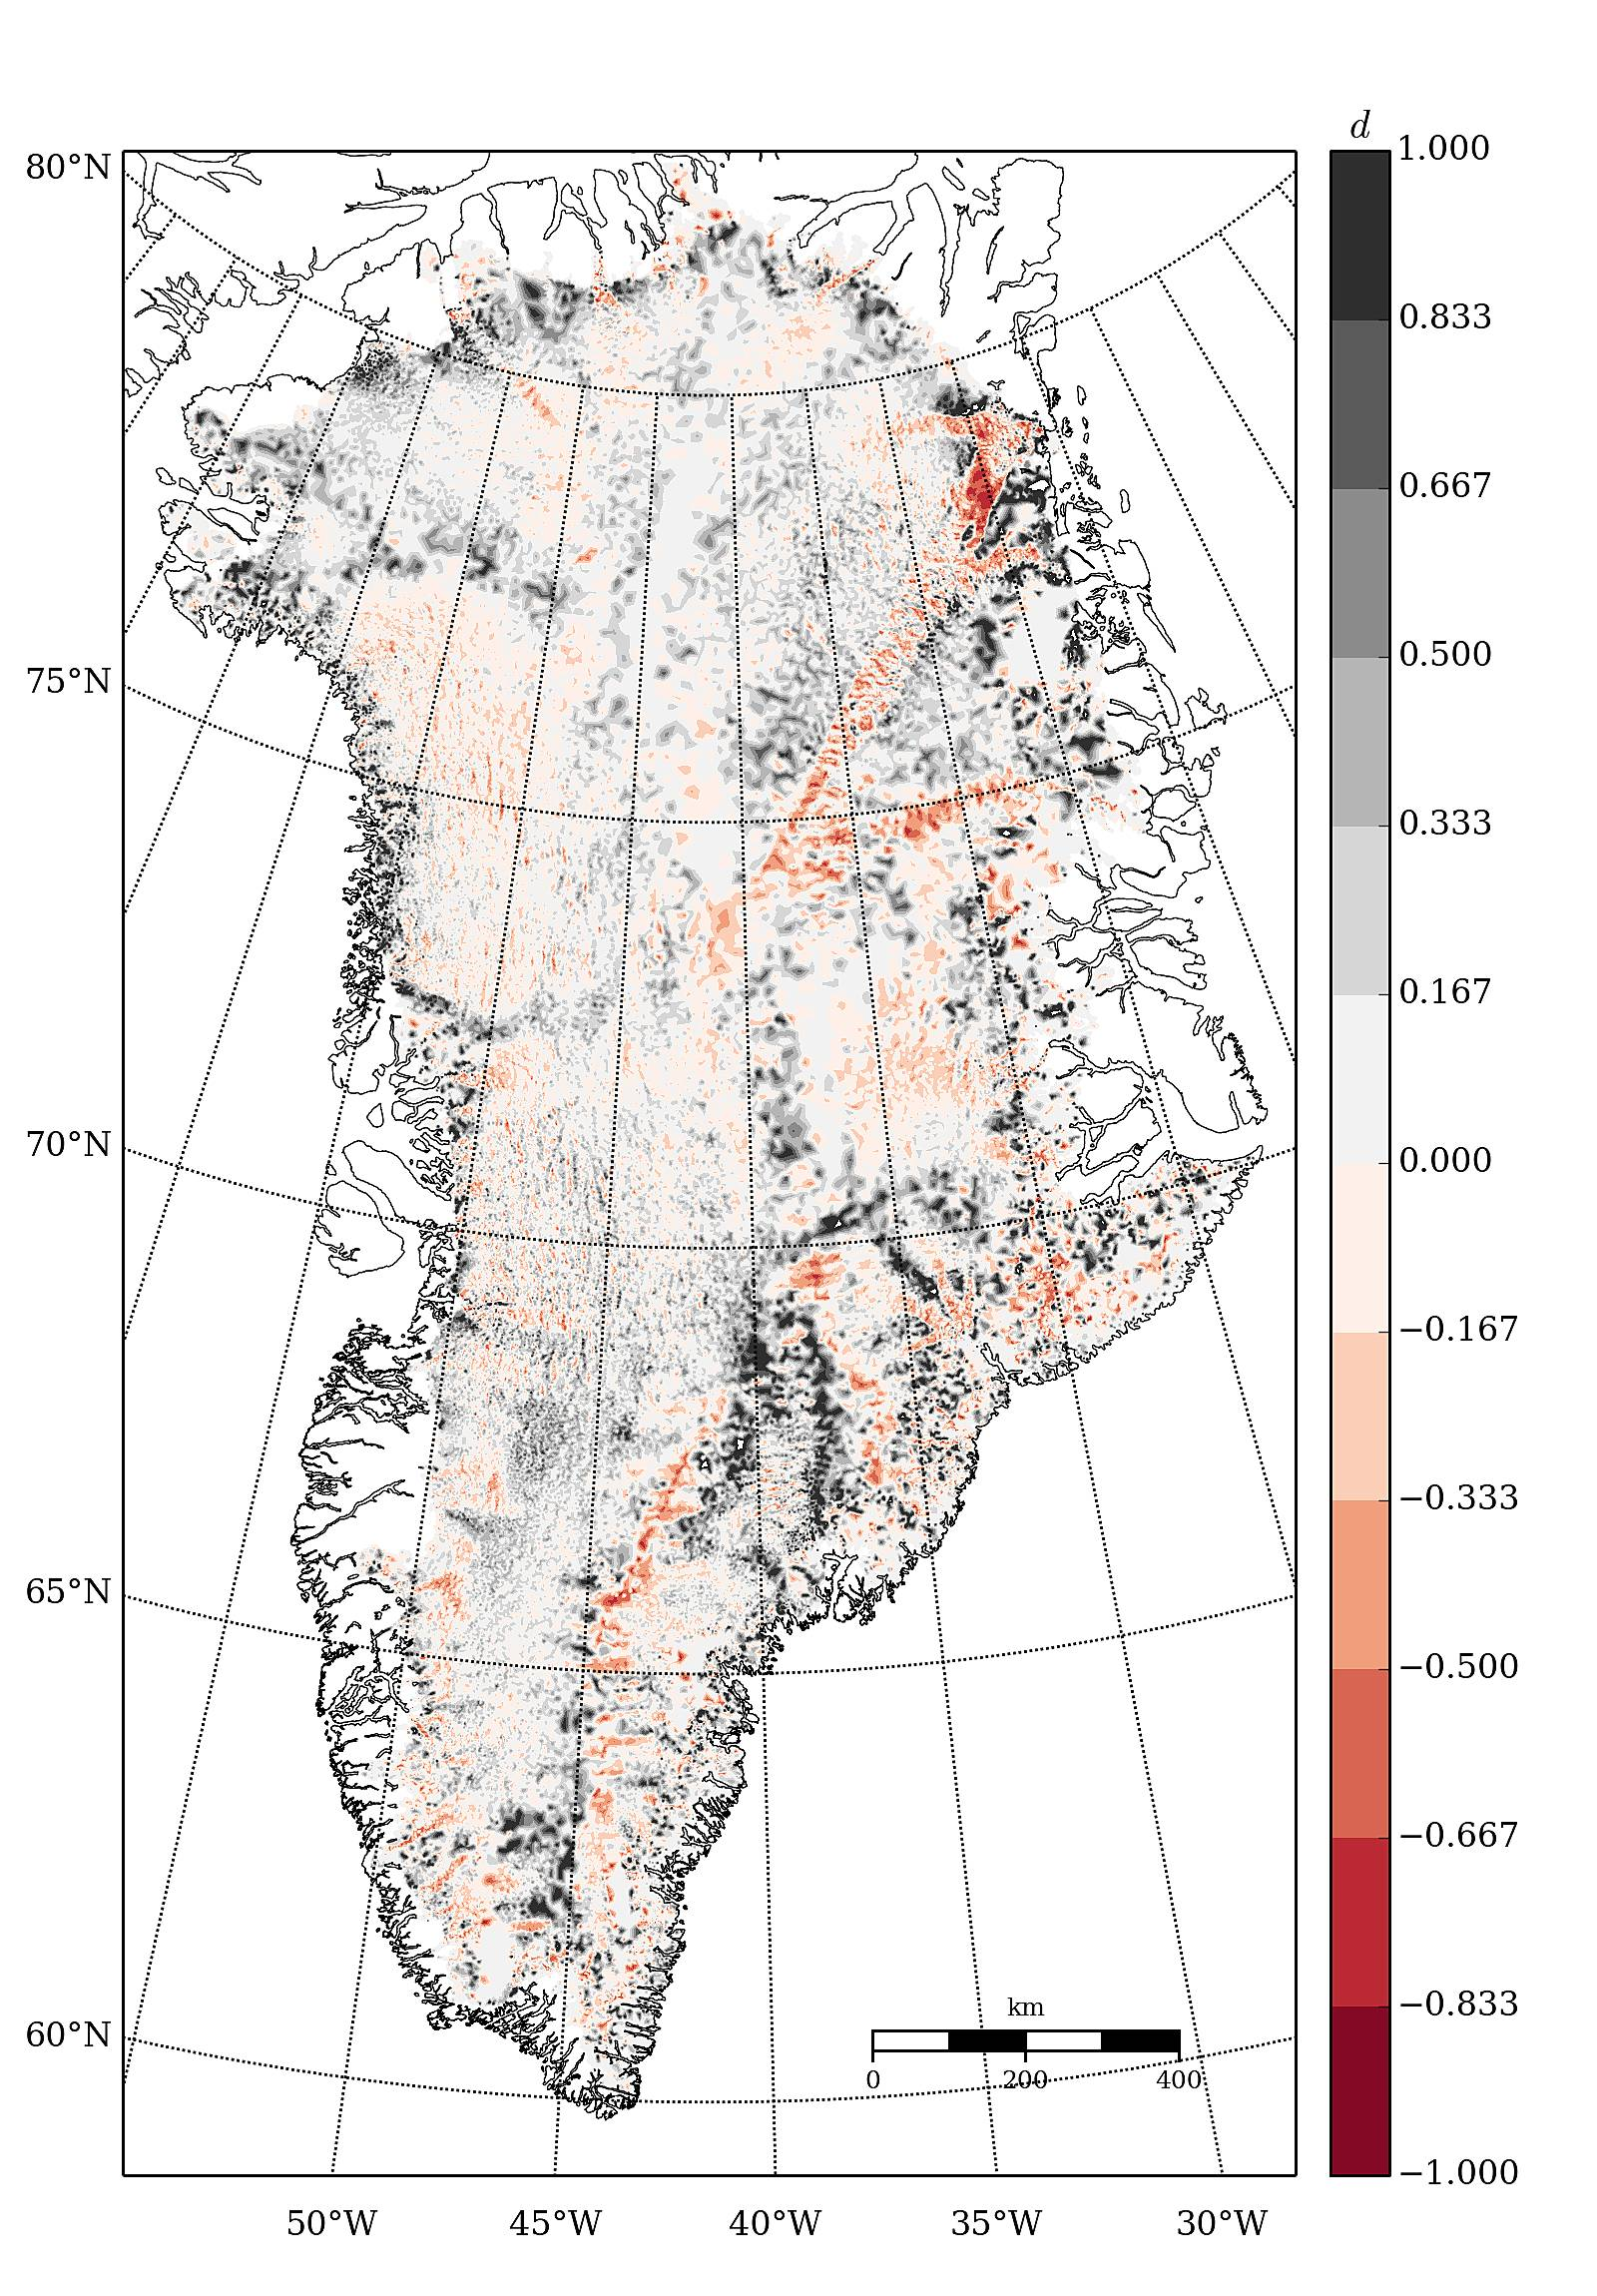
\includegraphics[width=1.0\textwidth]{images/greenland/stats/GLM_resid_no_velocity.jpg}
  \end{minipage}
  \begin{minipage}[b]{0.99\linewidth}
    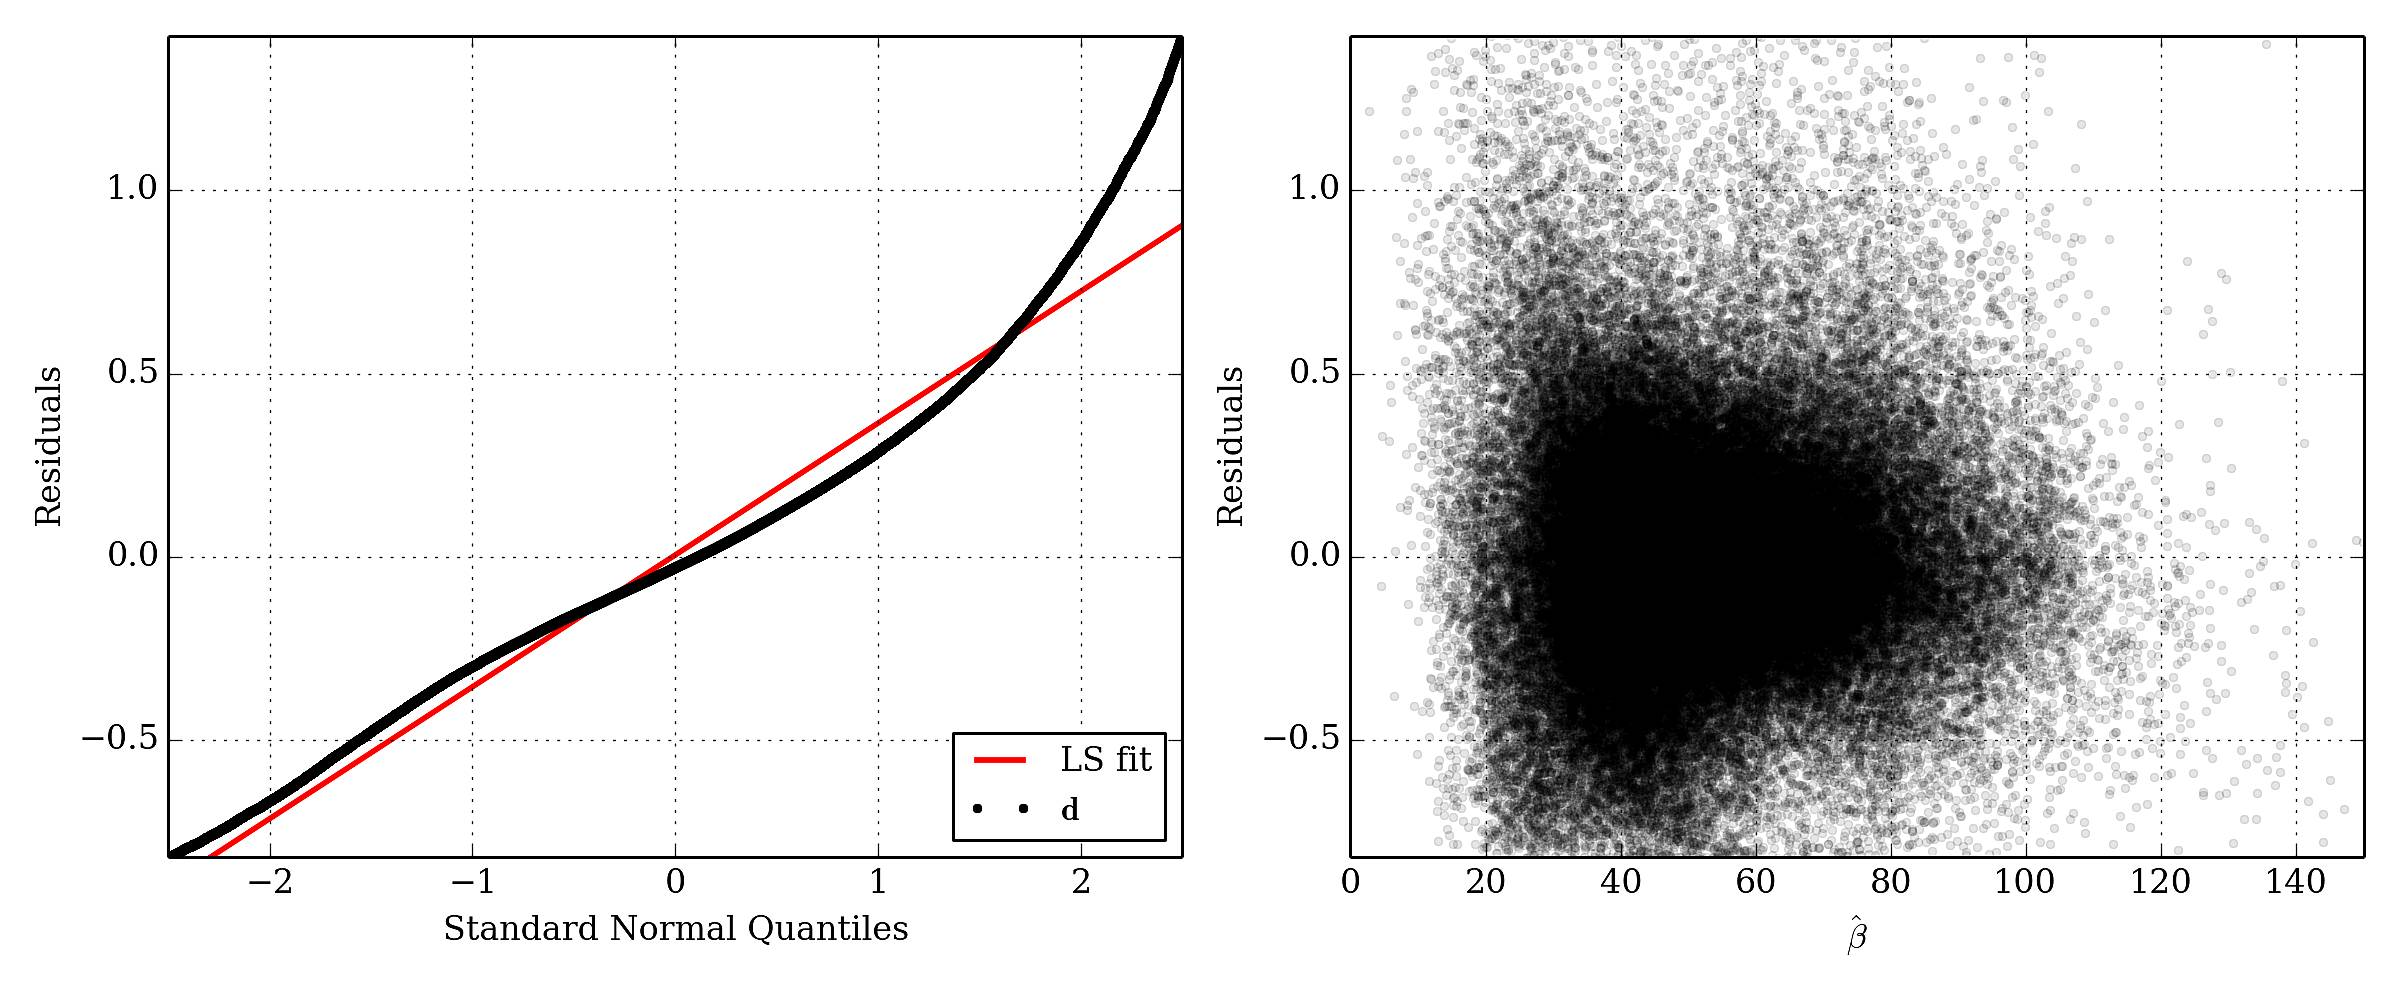
\includegraphics[width=1.0\textwidth]{images/greenland/stats/GLM_resid-NQ_no_velocity.jpg}
  \end{minipage}
  \caption[]{GLM model fit $\bm{\hat{\beta}}$ and residual $\mathbf{d}$, excluding any variable derived from and including $\mathbf{U}$ (except $T_B$ and $M_B$) from $\mat{X}$.}
\end{figure}

\begin{figure}
  \centering
  \begin{minipage}[b]{0.47\linewidth}
    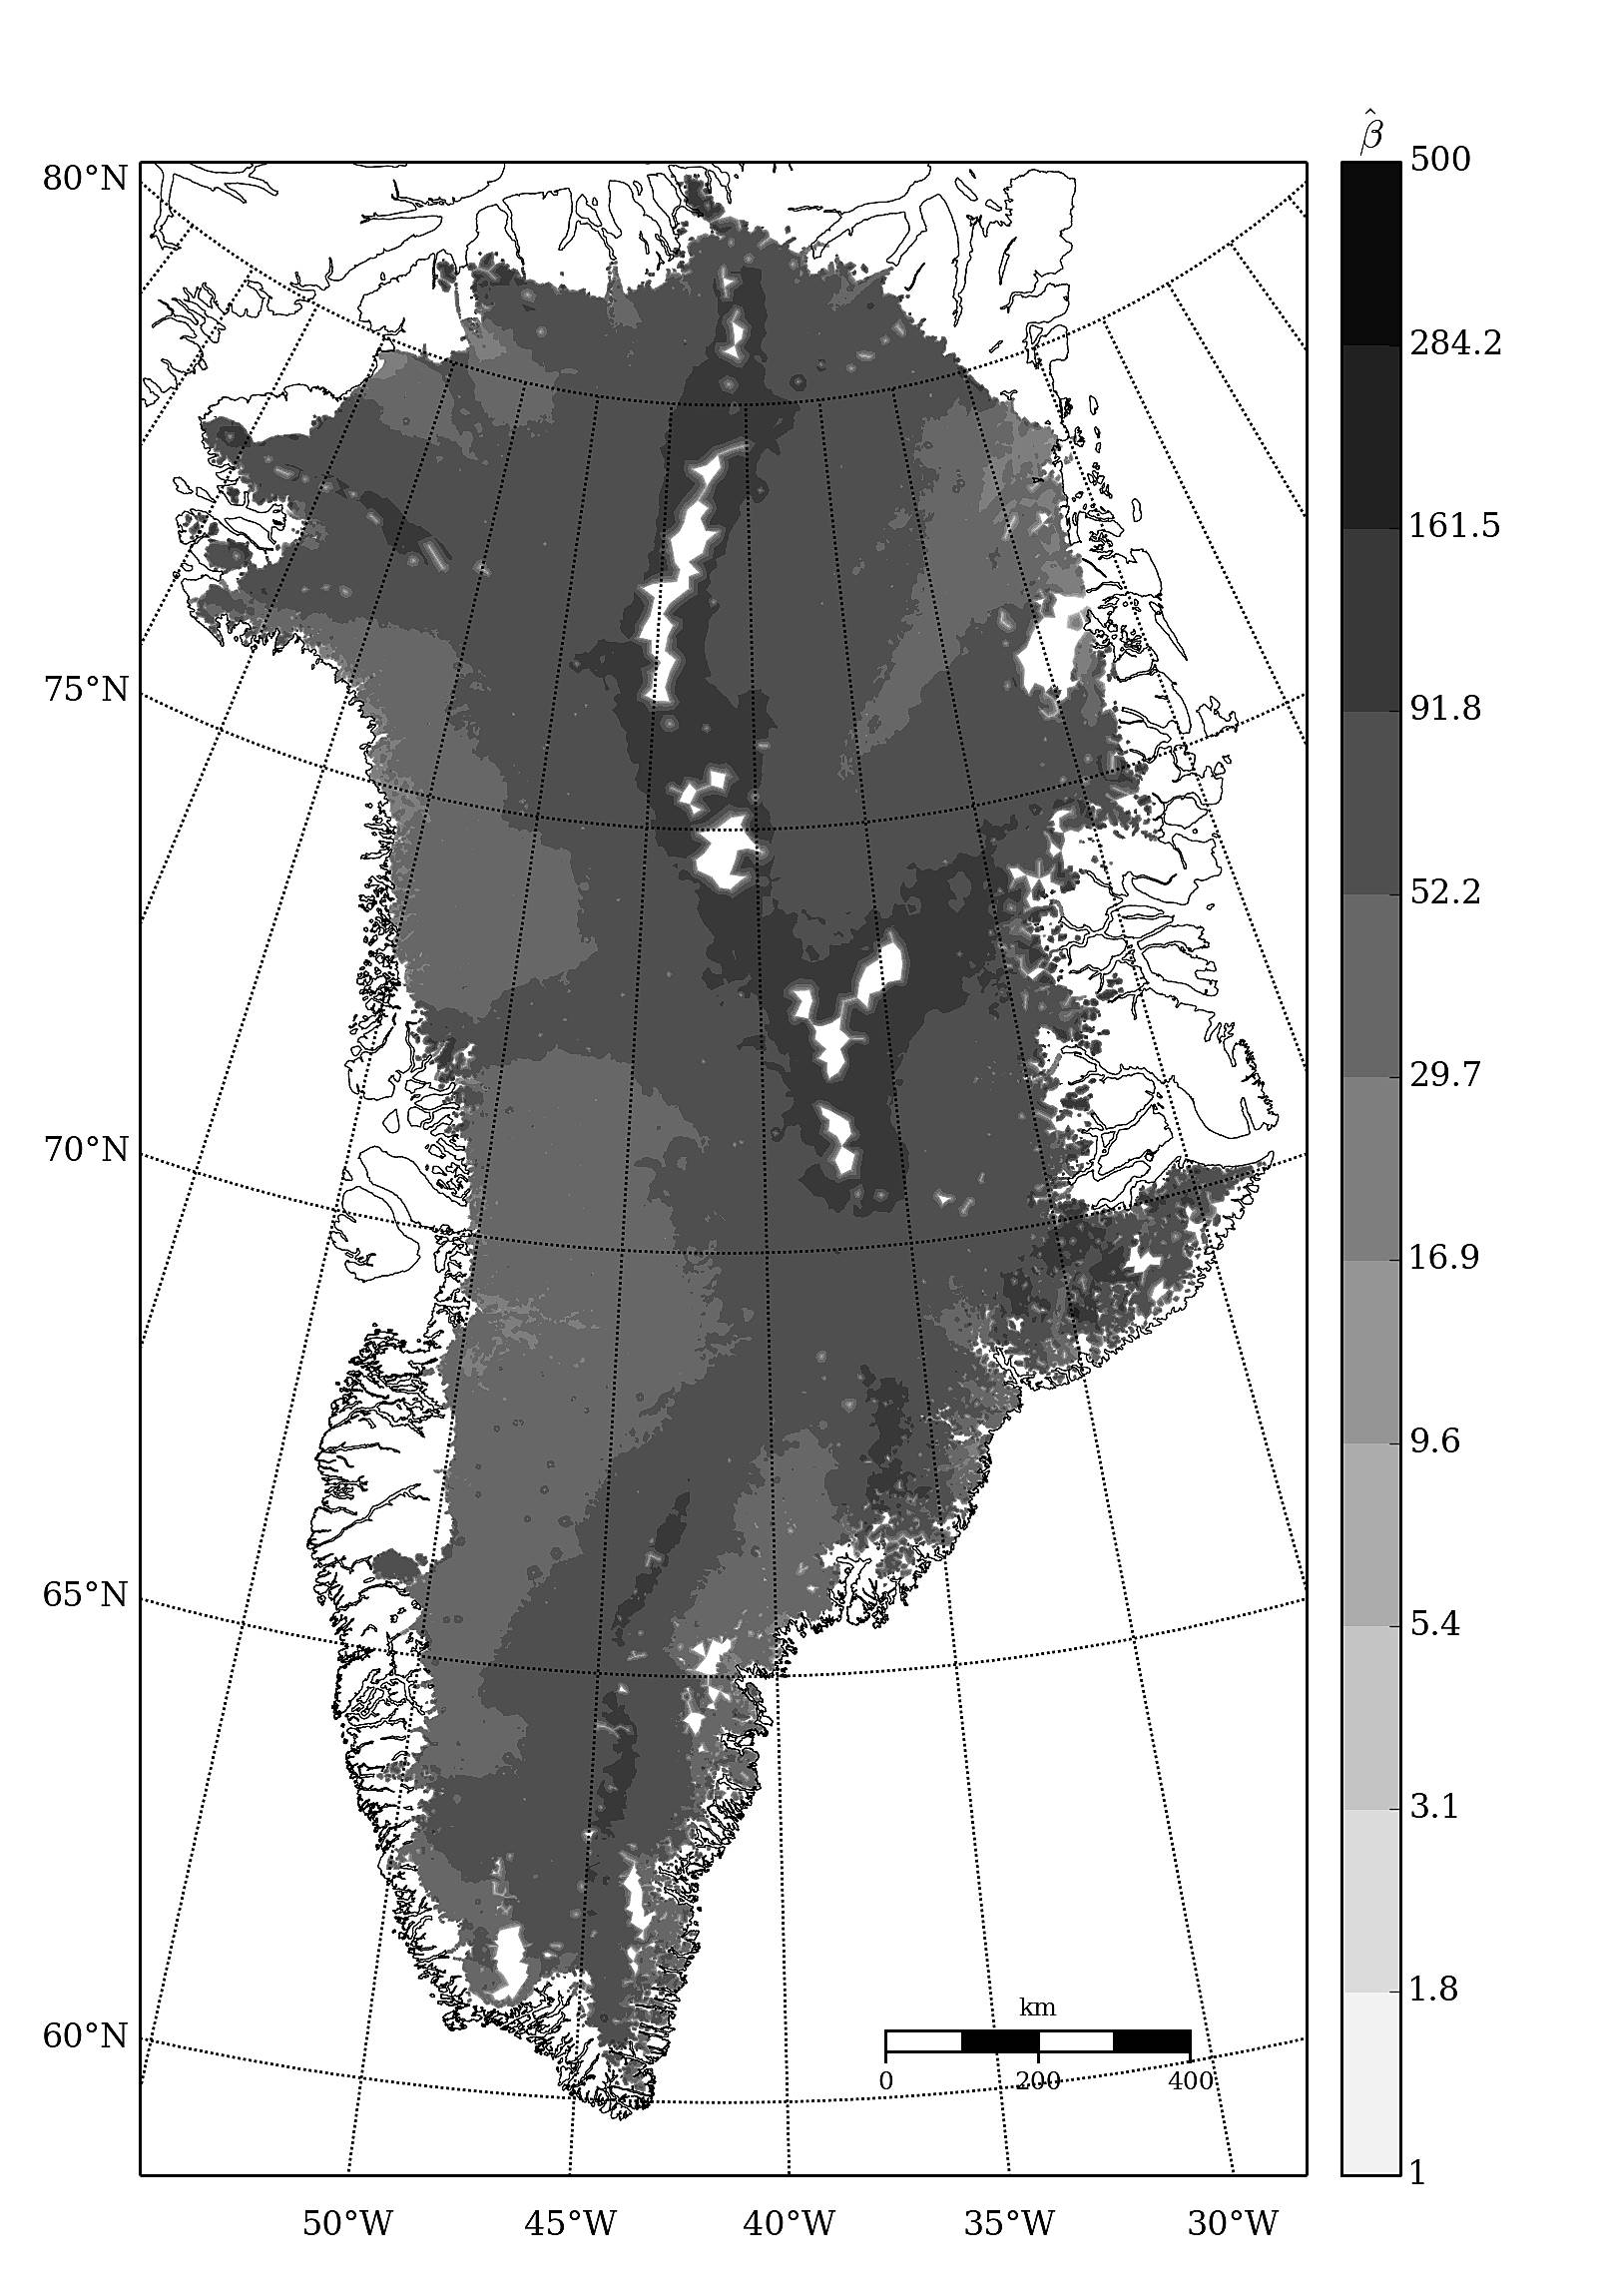
\includegraphics[width=1.0\textwidth]{images/greenland/stats/GLM_beta_ind_only.jpg}
  \end{minipage}
  \quad
  \begin{minipage}[b]{0.47\linewidth}
    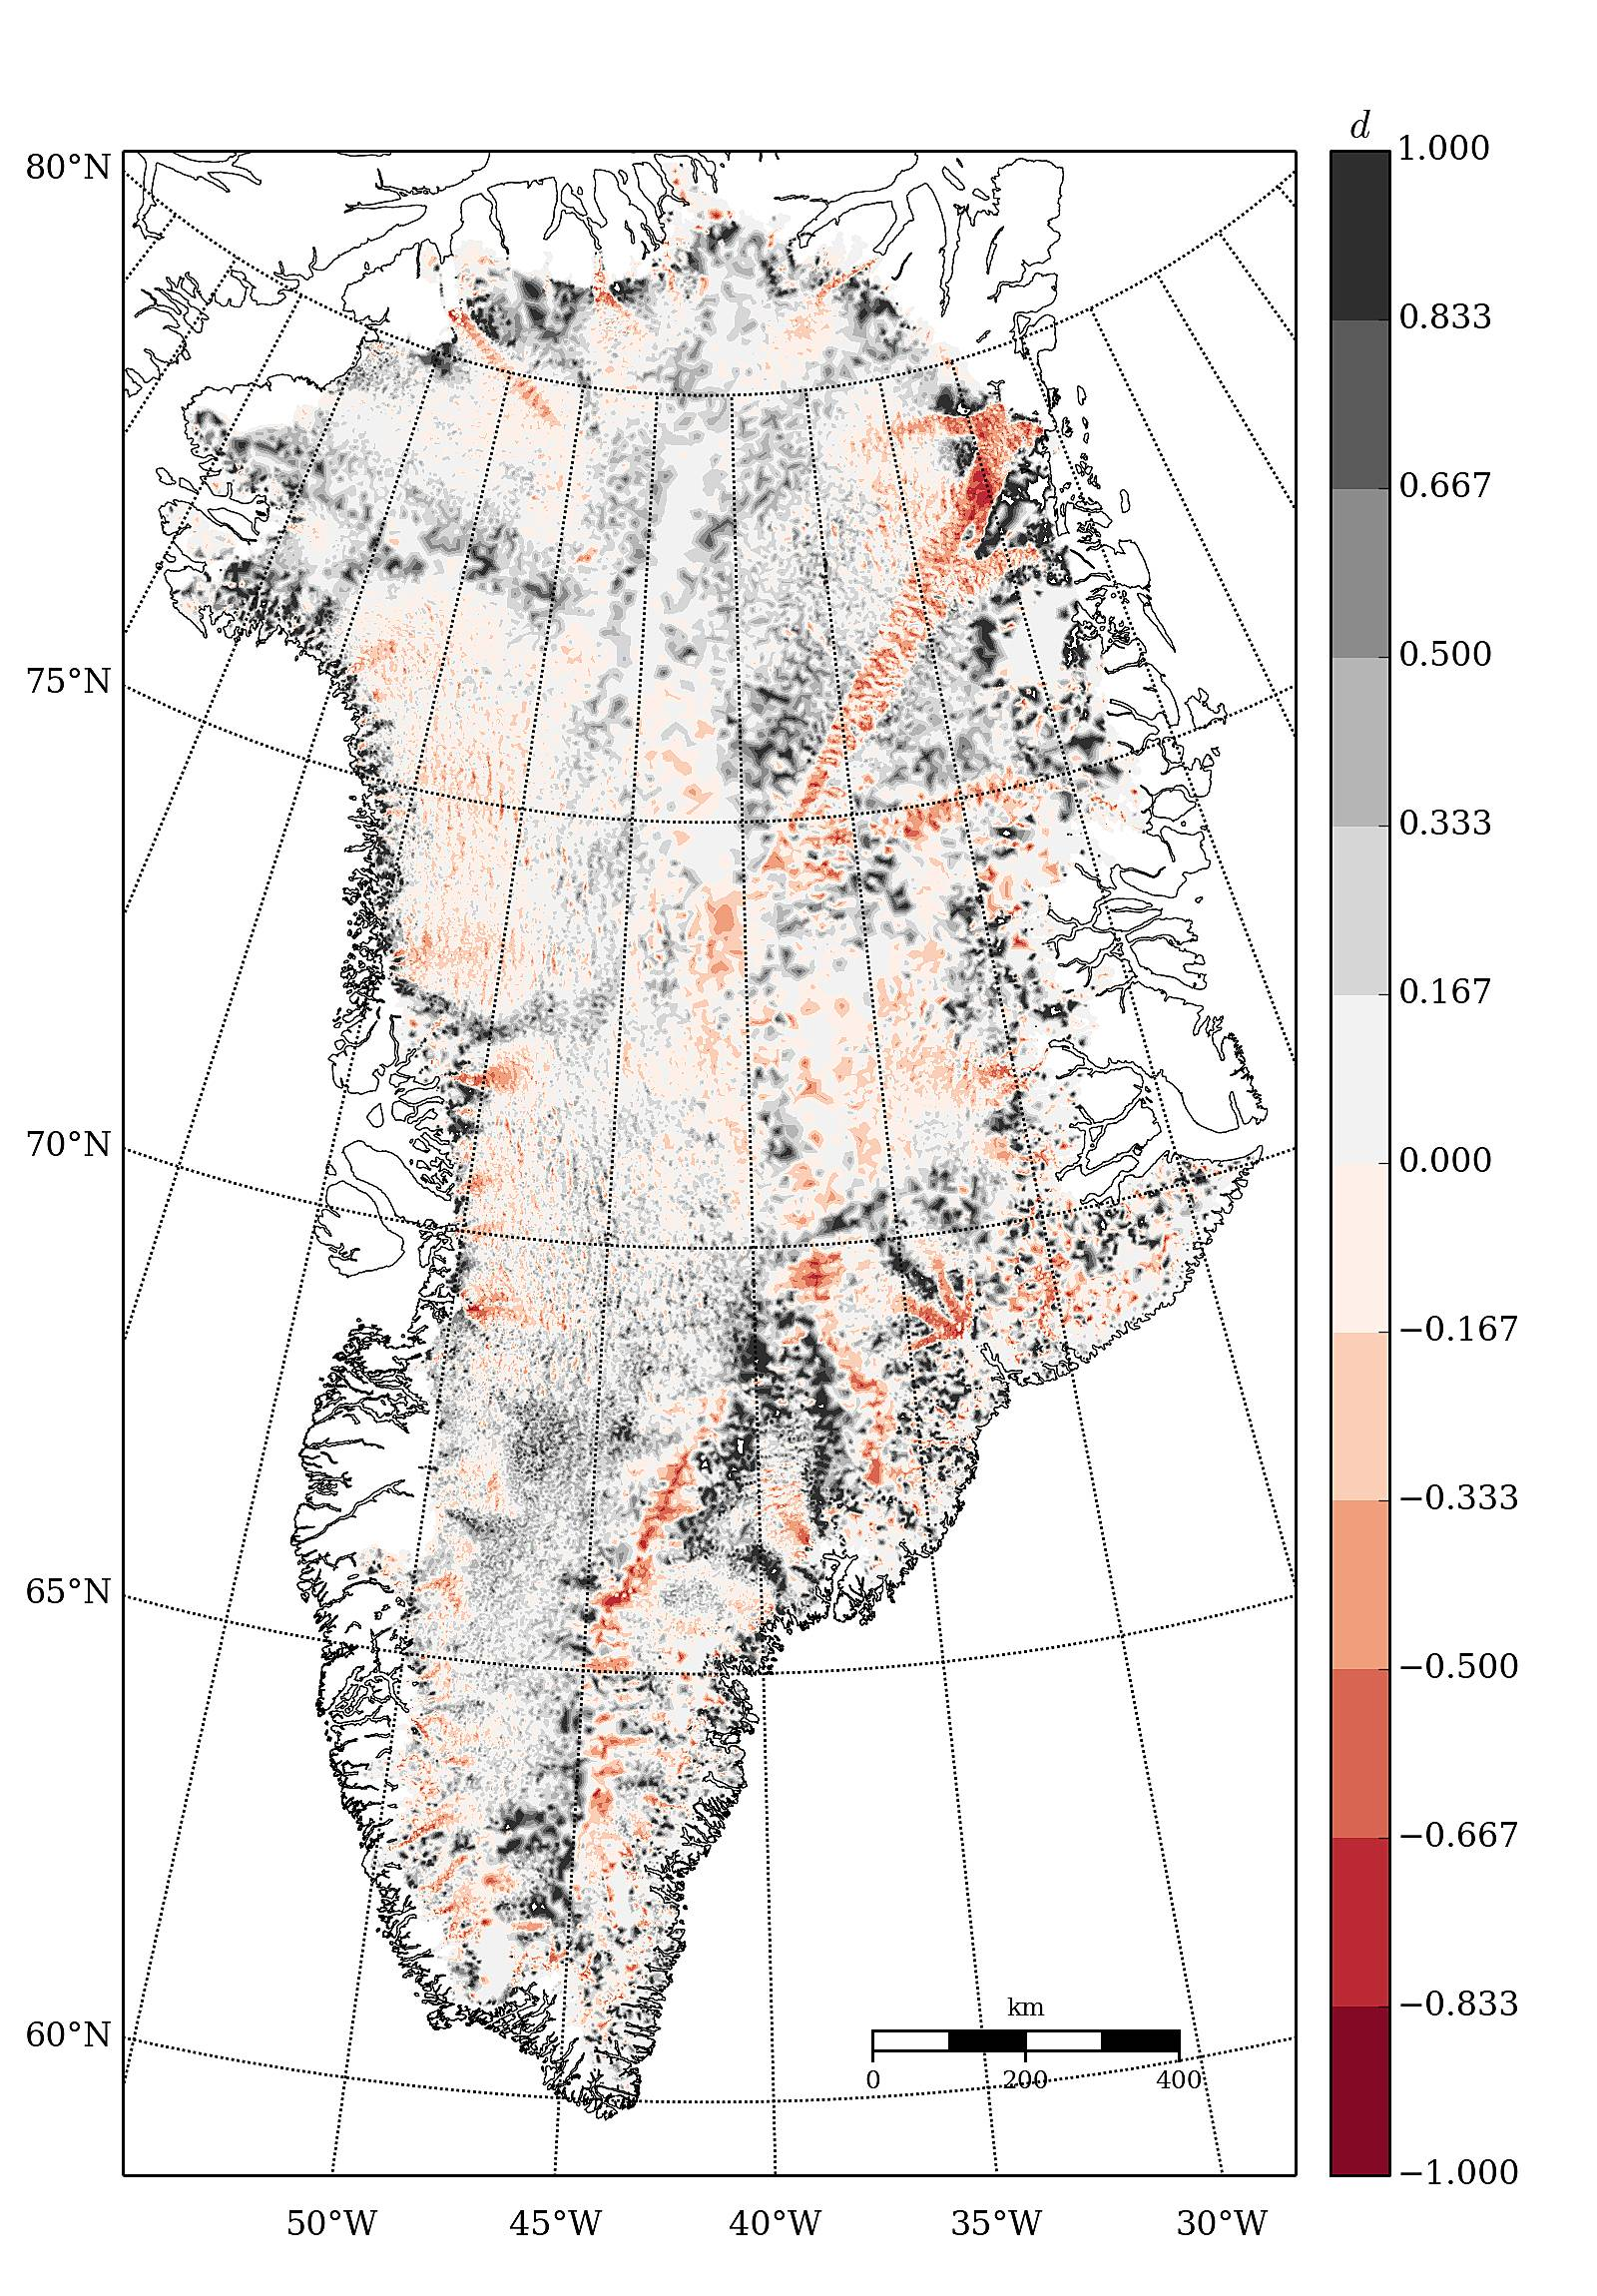
\includegraphics[width=1.0\textwidth]{images/greenland/stats/GLM_resid_ind_only.jpg}
  \end{minipage}
  \begin{minipage}[b]{0.99\linewidth}
    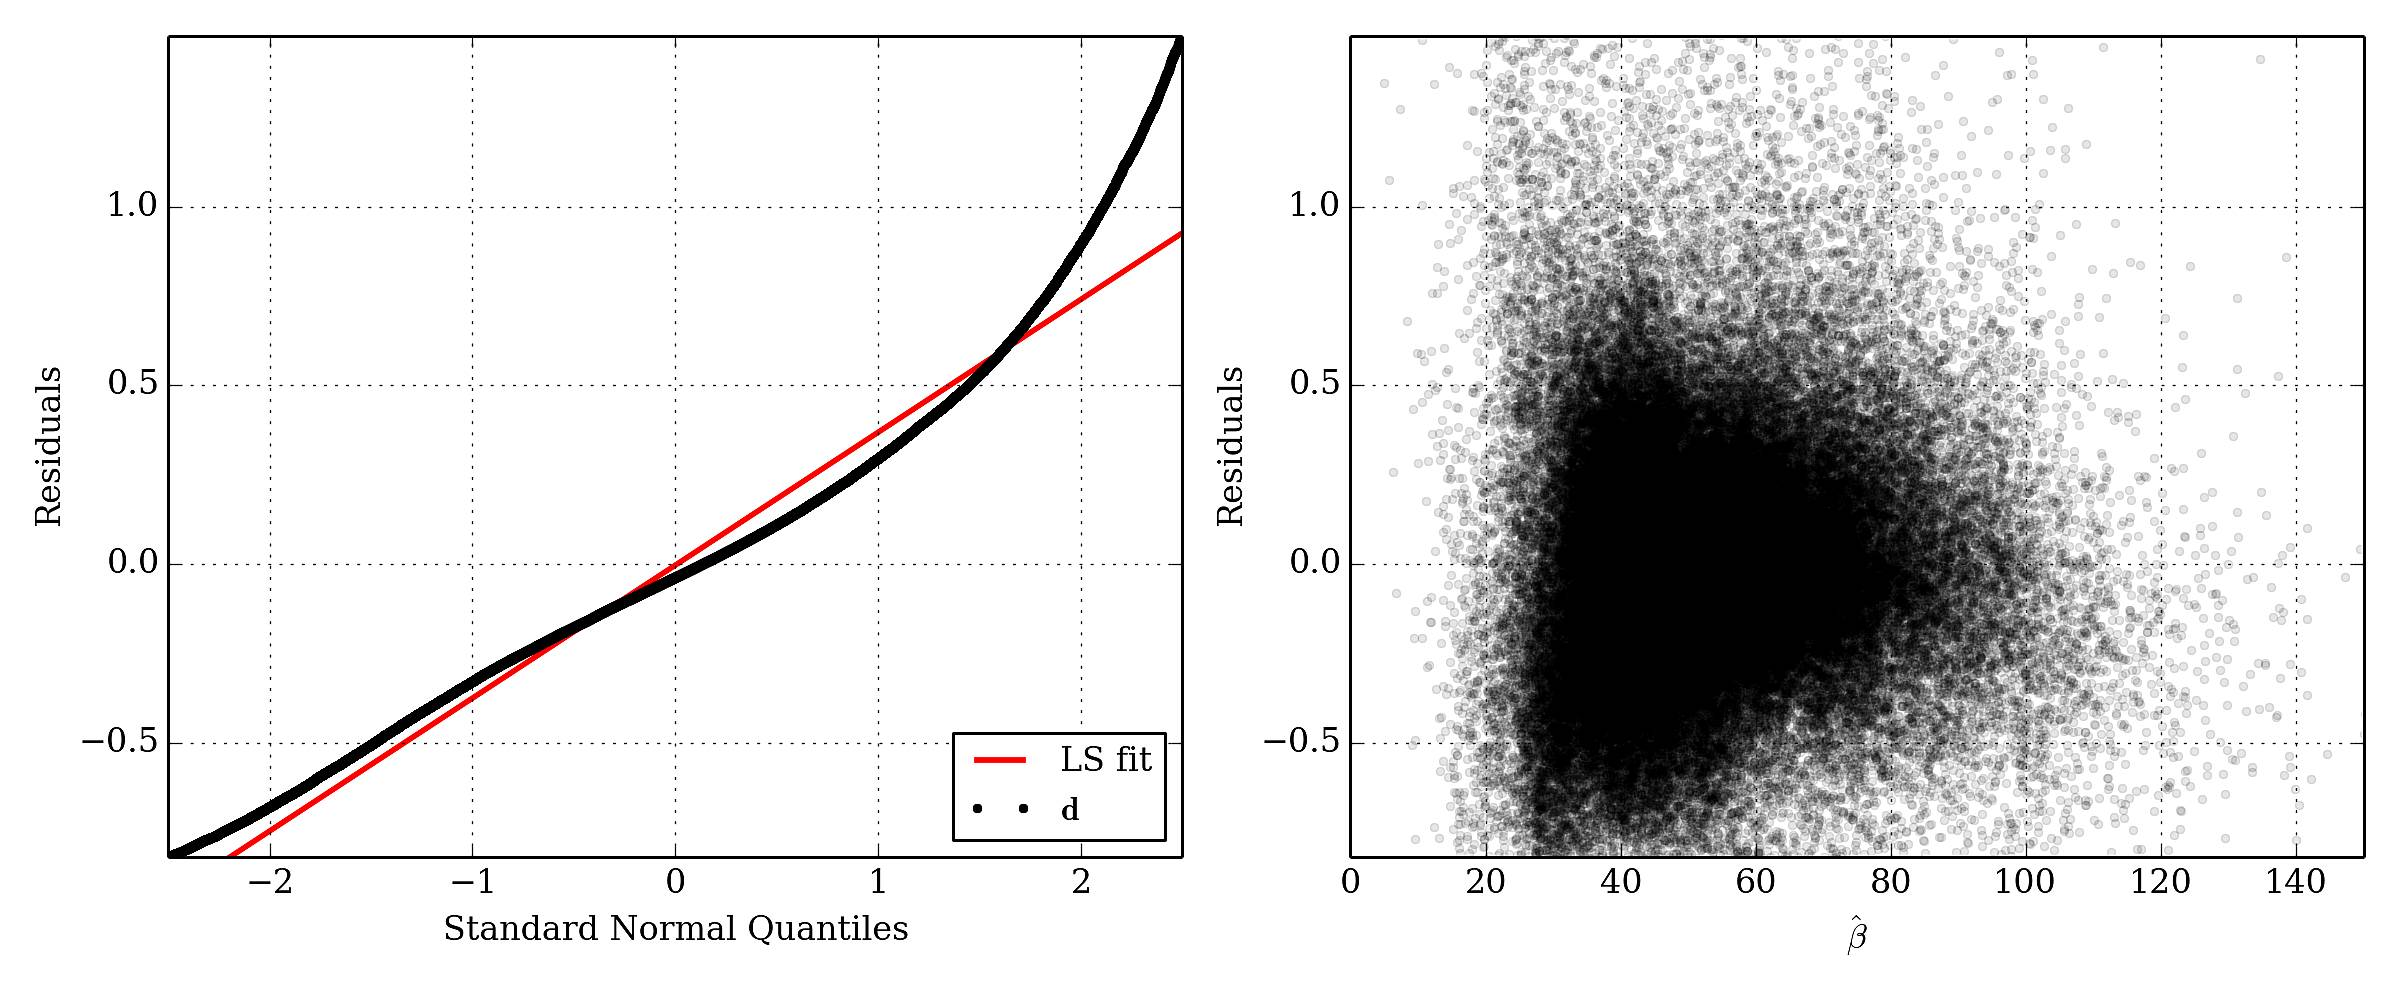
\includegraphics[width=1.0\textwidth]{images/greenland/stats/GLM_resid-NQ_ind_only.jpg}
  \end{minipage}
  \caption[]{GLM model fit $\bm{\hat{\beta}}$ and residual $\mathbf{d}$, including only independent variables in $\mat{X}$.}
\end{figure}



\begin{table}[H]
\centering
\normalsize
\begin{tabular}{l|l|l}
  & $\bm{\beta}$ & $\bm{\hat{\beta}}$ \\
  \hline
$\mu$ & 52.6245 & 52.7069 \\
median & 48.4405 & 48.409 \\
$\sigma$ & 26.7237 & 22.7305 \\
IQR & 3.08544 & 4.12095 \\
$\sigma^2 / \mu$ & 13.5708 & 9.80283 \\
\end{tabular}
  \caption[]{\normalsize Useful statistics of the data $\bm{\beta}$ and predicted values $\bm{\hat{\beta}}$.}
\end{table}

%% results ====================================================================
\section{GLM-derived traction}

Once the adjoint process is completed, we replace the assimilated basal traction with the GLM-derived basal traction and solve the thermo-mechanically coupled system once more.  These results are shown below.

\begin{figure}
  \centering
  \begin{minipage}[b]{1.00\linewidth}
    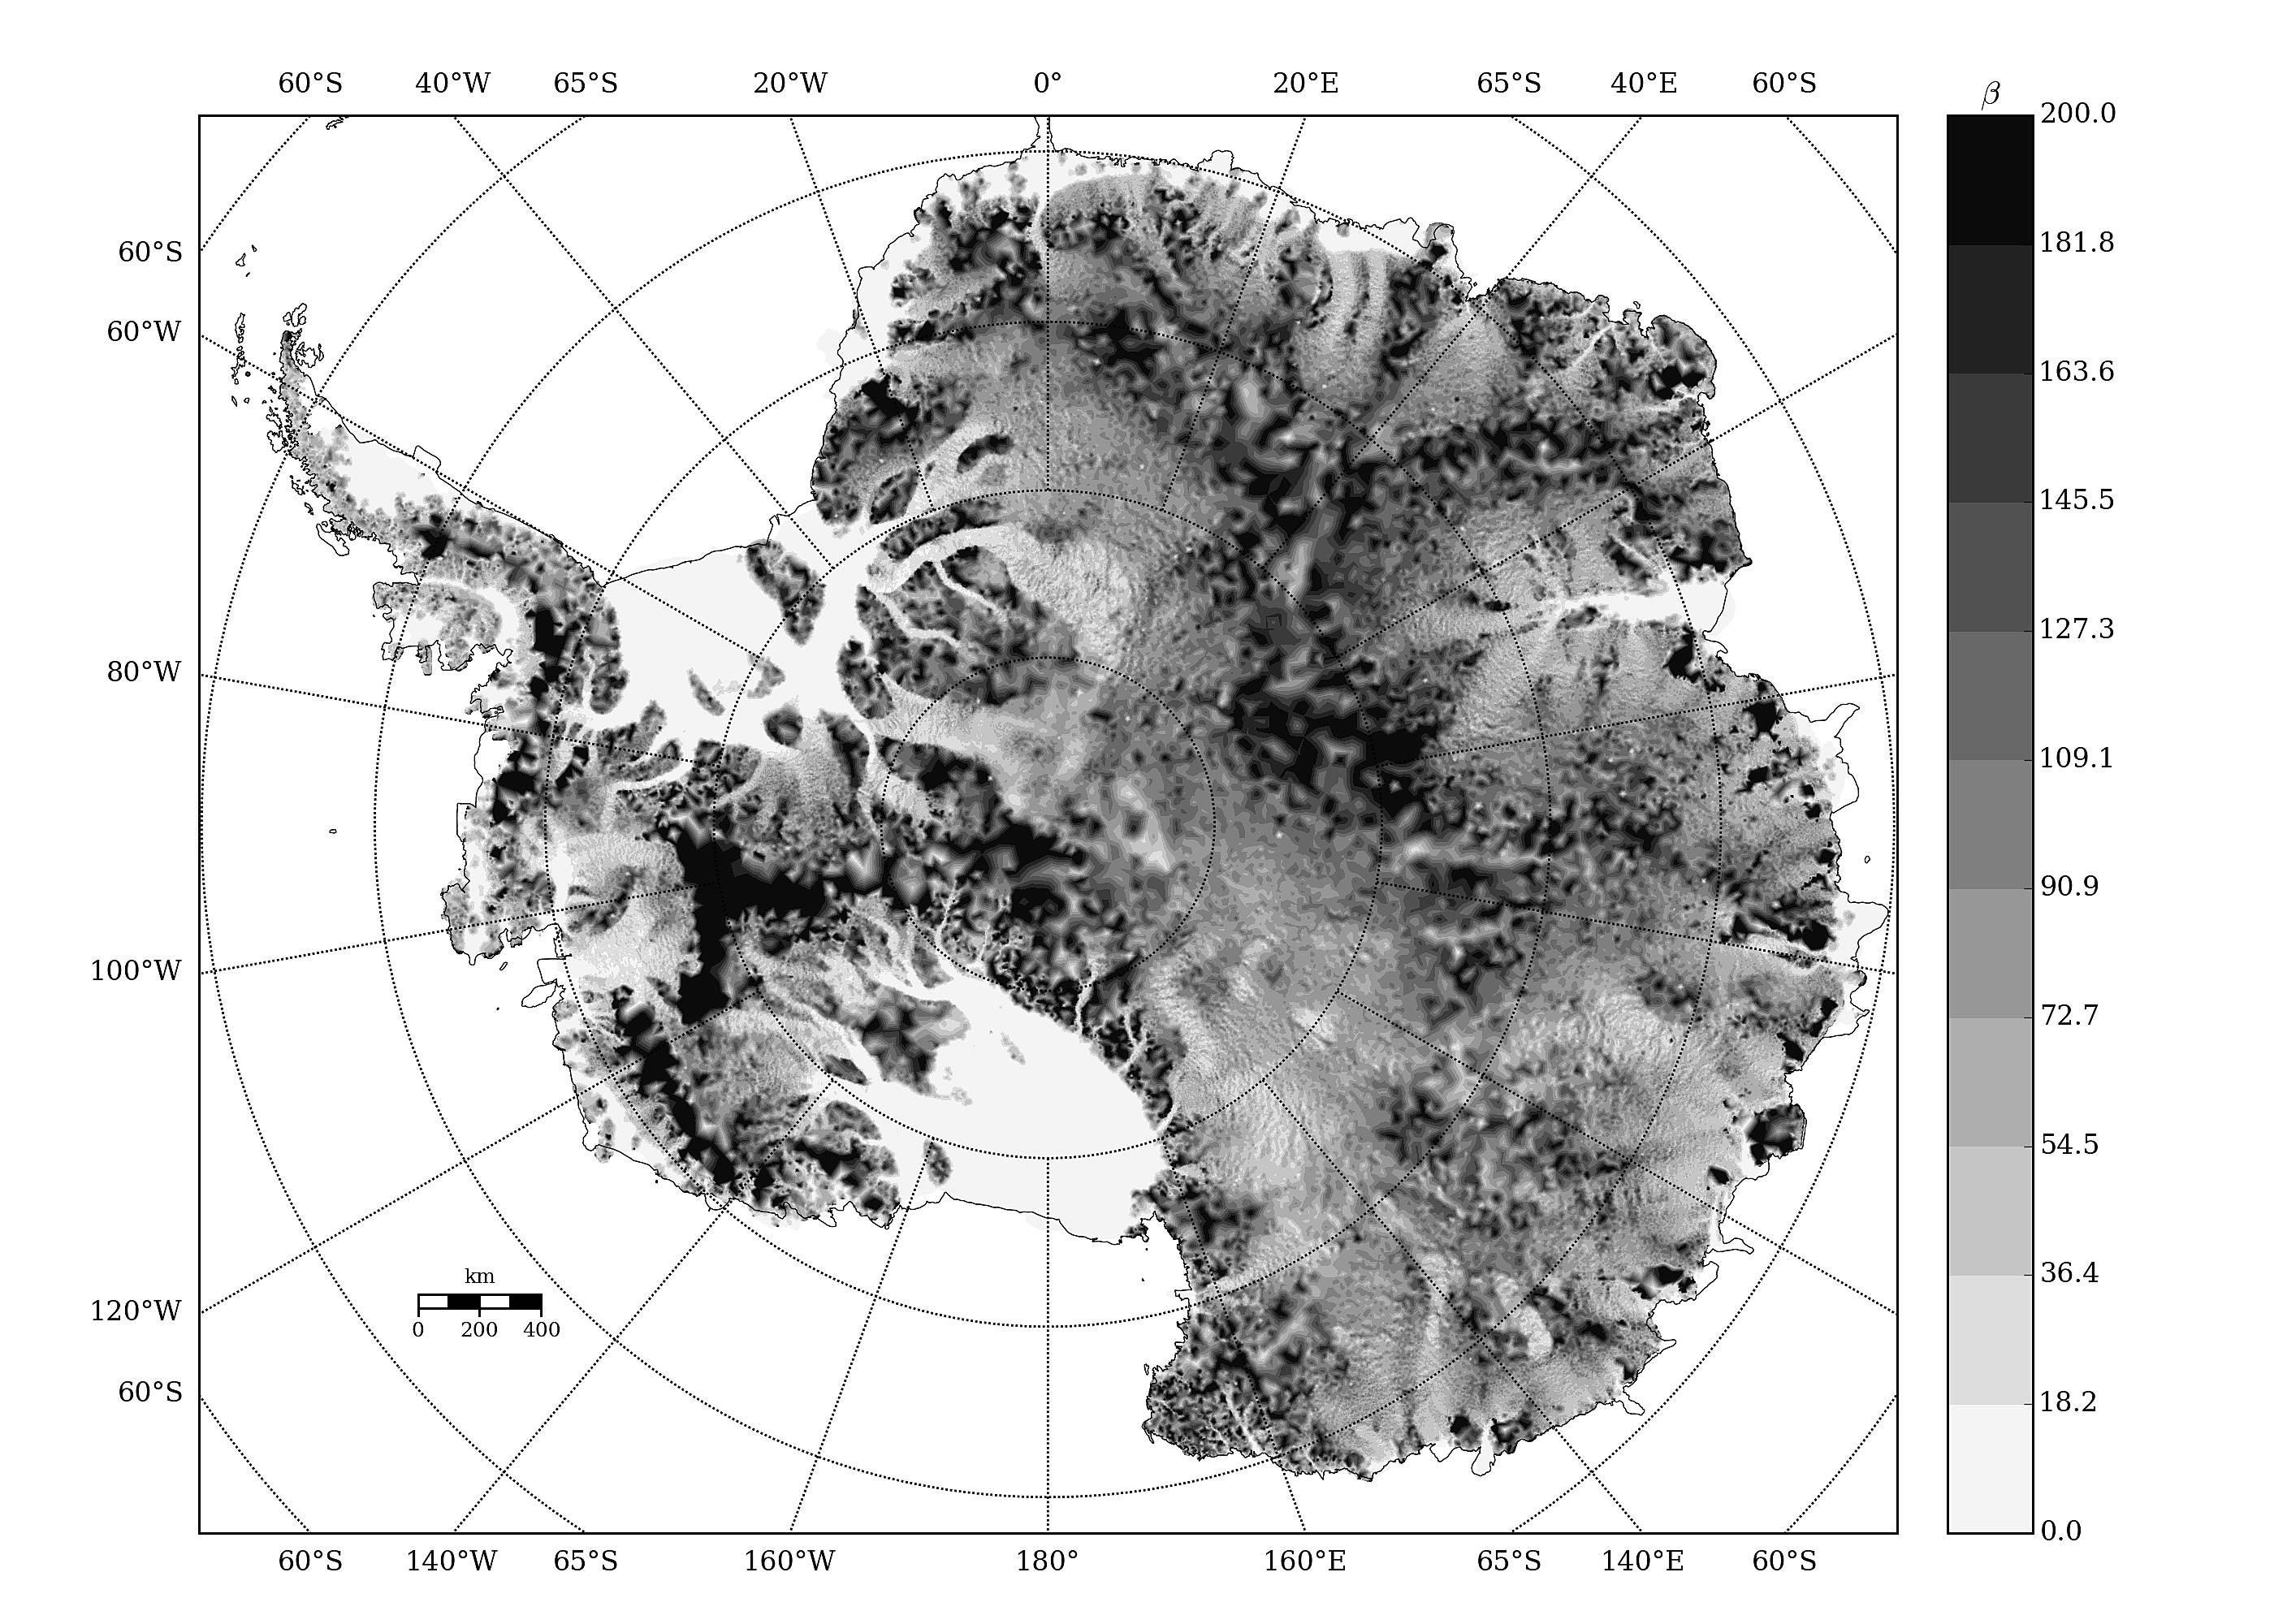
\includegraphics[width=1.0\textwidth]{images/antarctica/model/beta.jpg}
  \end{minipage}
	\caption[]{Basal traction field $\beta$ (Pa a/m)$^{1/2}$ resulting from the adjoint-assimilation process.}
\end{figure}


\begin{figure}
  \centering
  \begin{minipage}[b]{1.00\linewidth}
    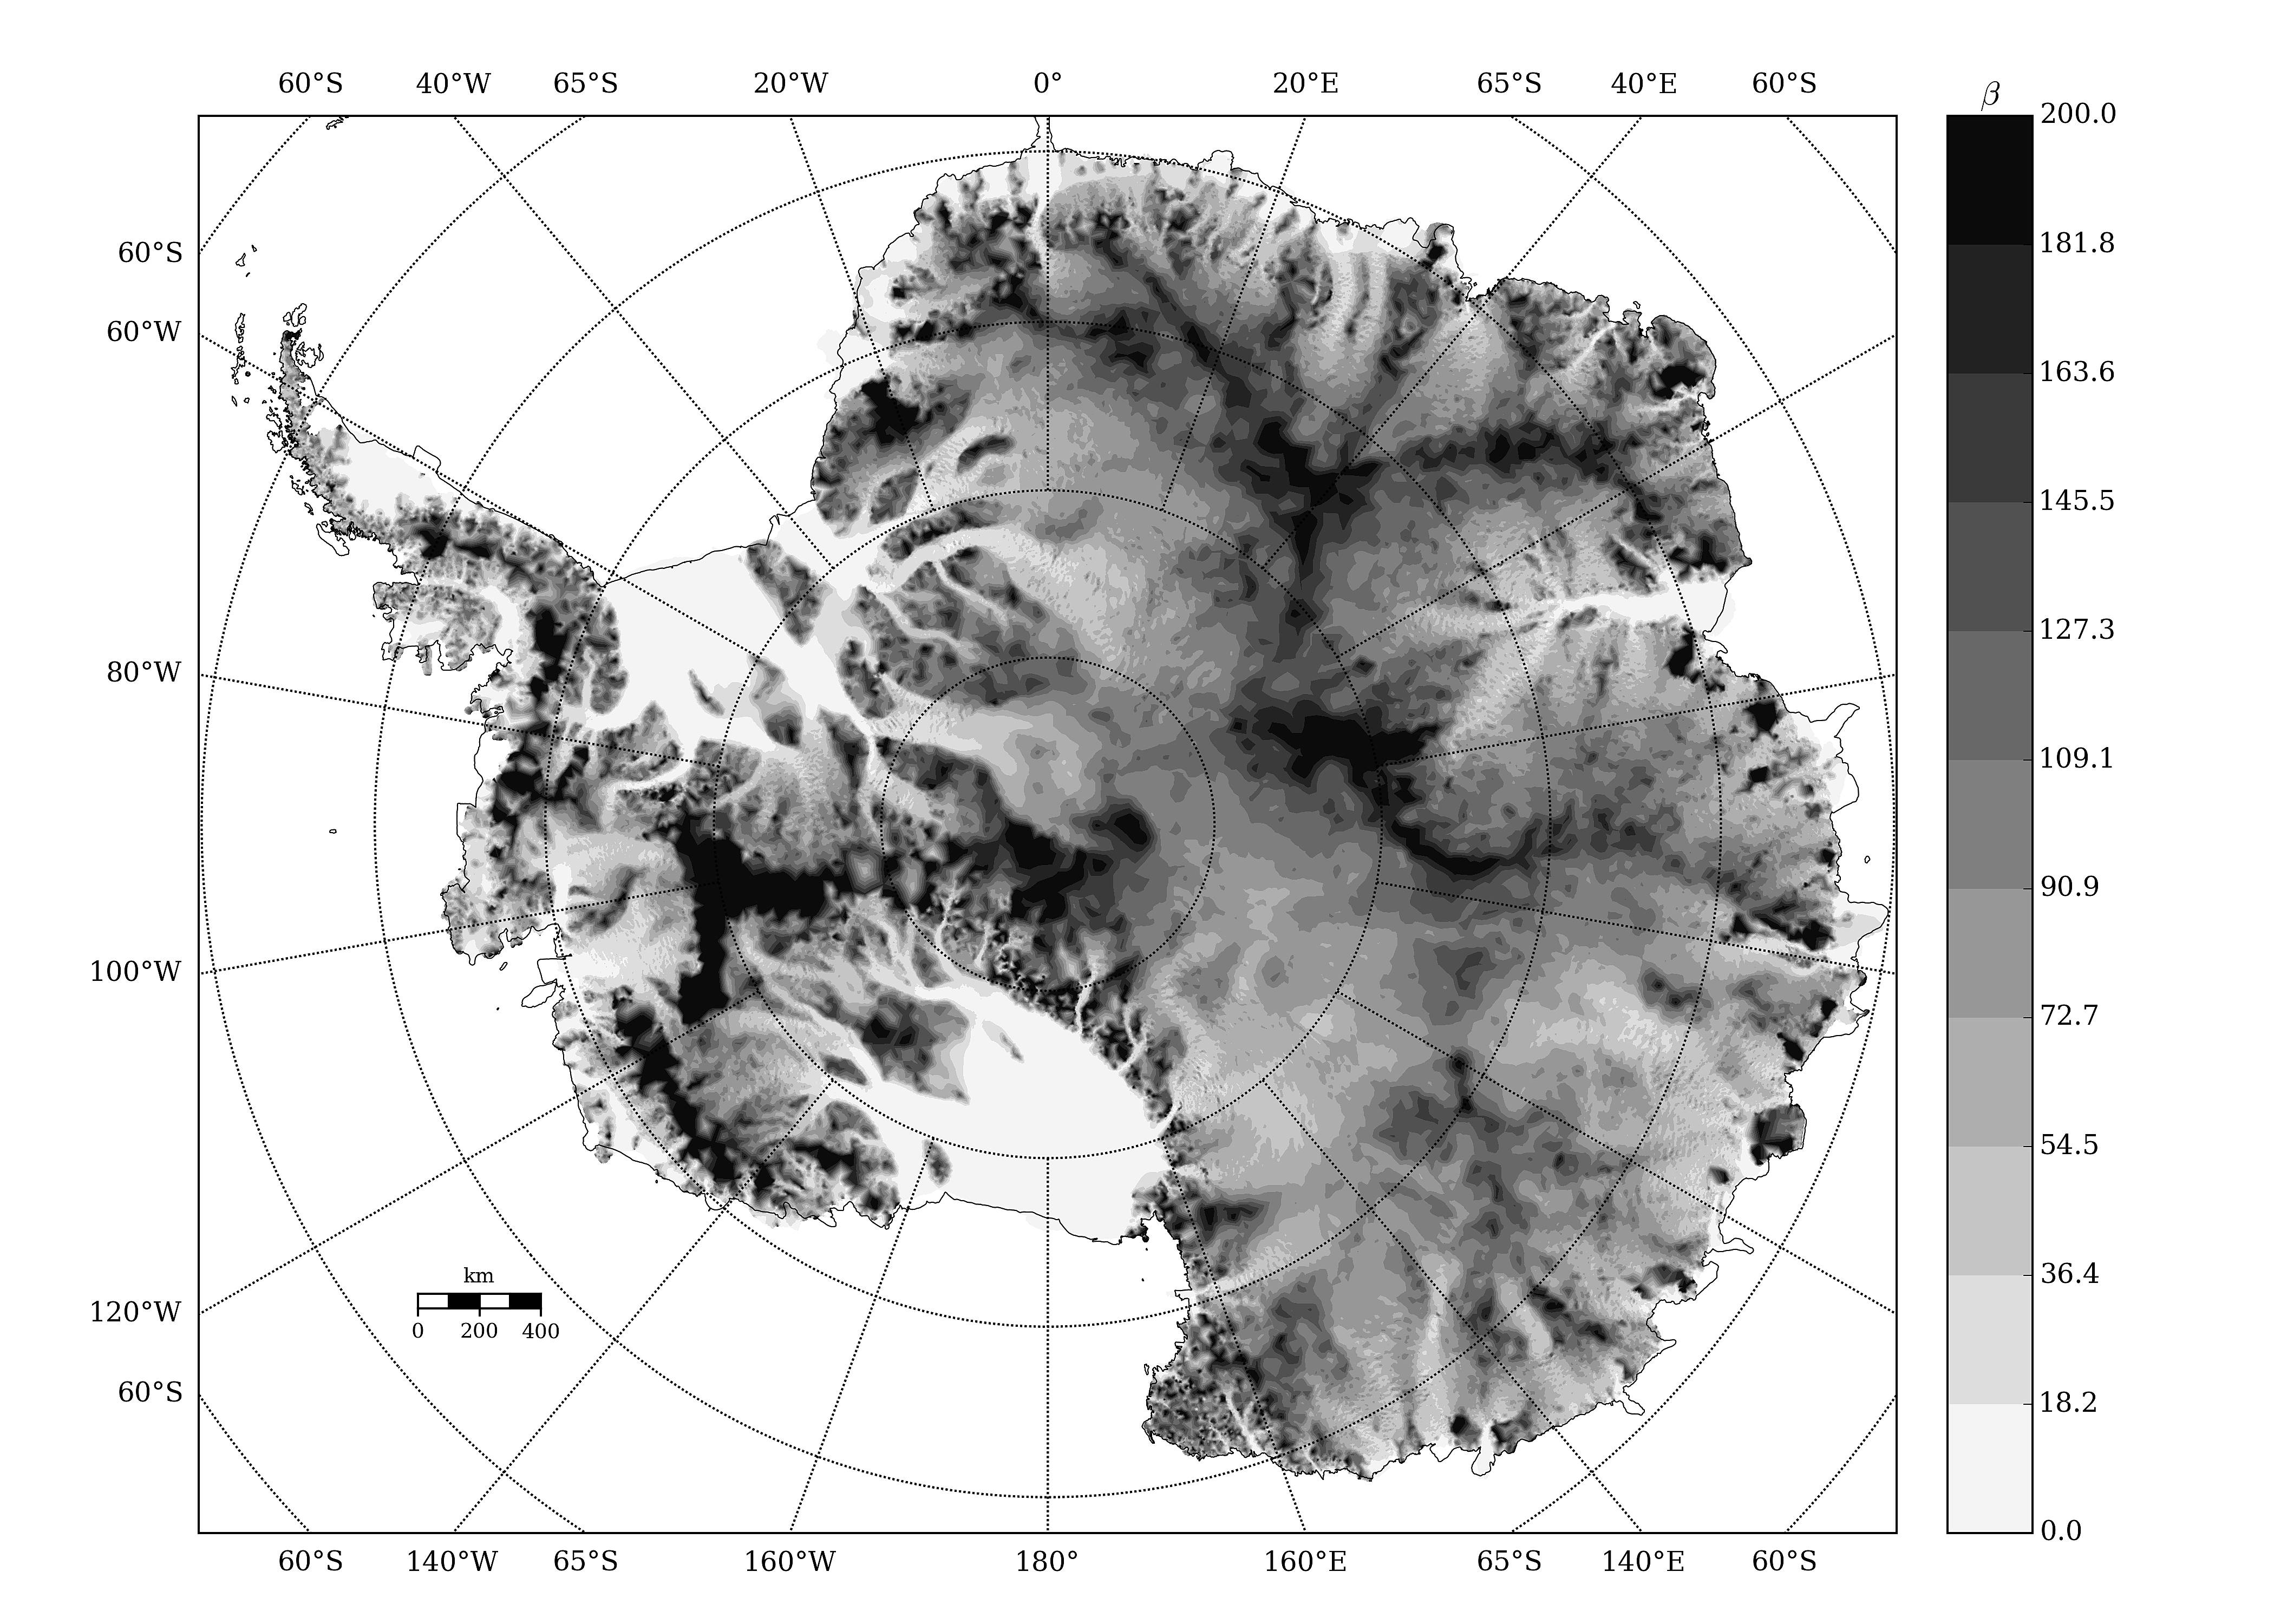
\includegraphics[width=1.0\textwidth]{images/antarctica/stats/GLM_beta_U.jpg}
  \end{minipage}
	\caption[]{GLM-derived basal traction in (Pa a/m)$^{1/2}$ derived with $\mathbf{u}_B$.}
\end{figure}


\begin{figure}
  \centering
  \begin{minipage}[b]{1.00\linewidth}
    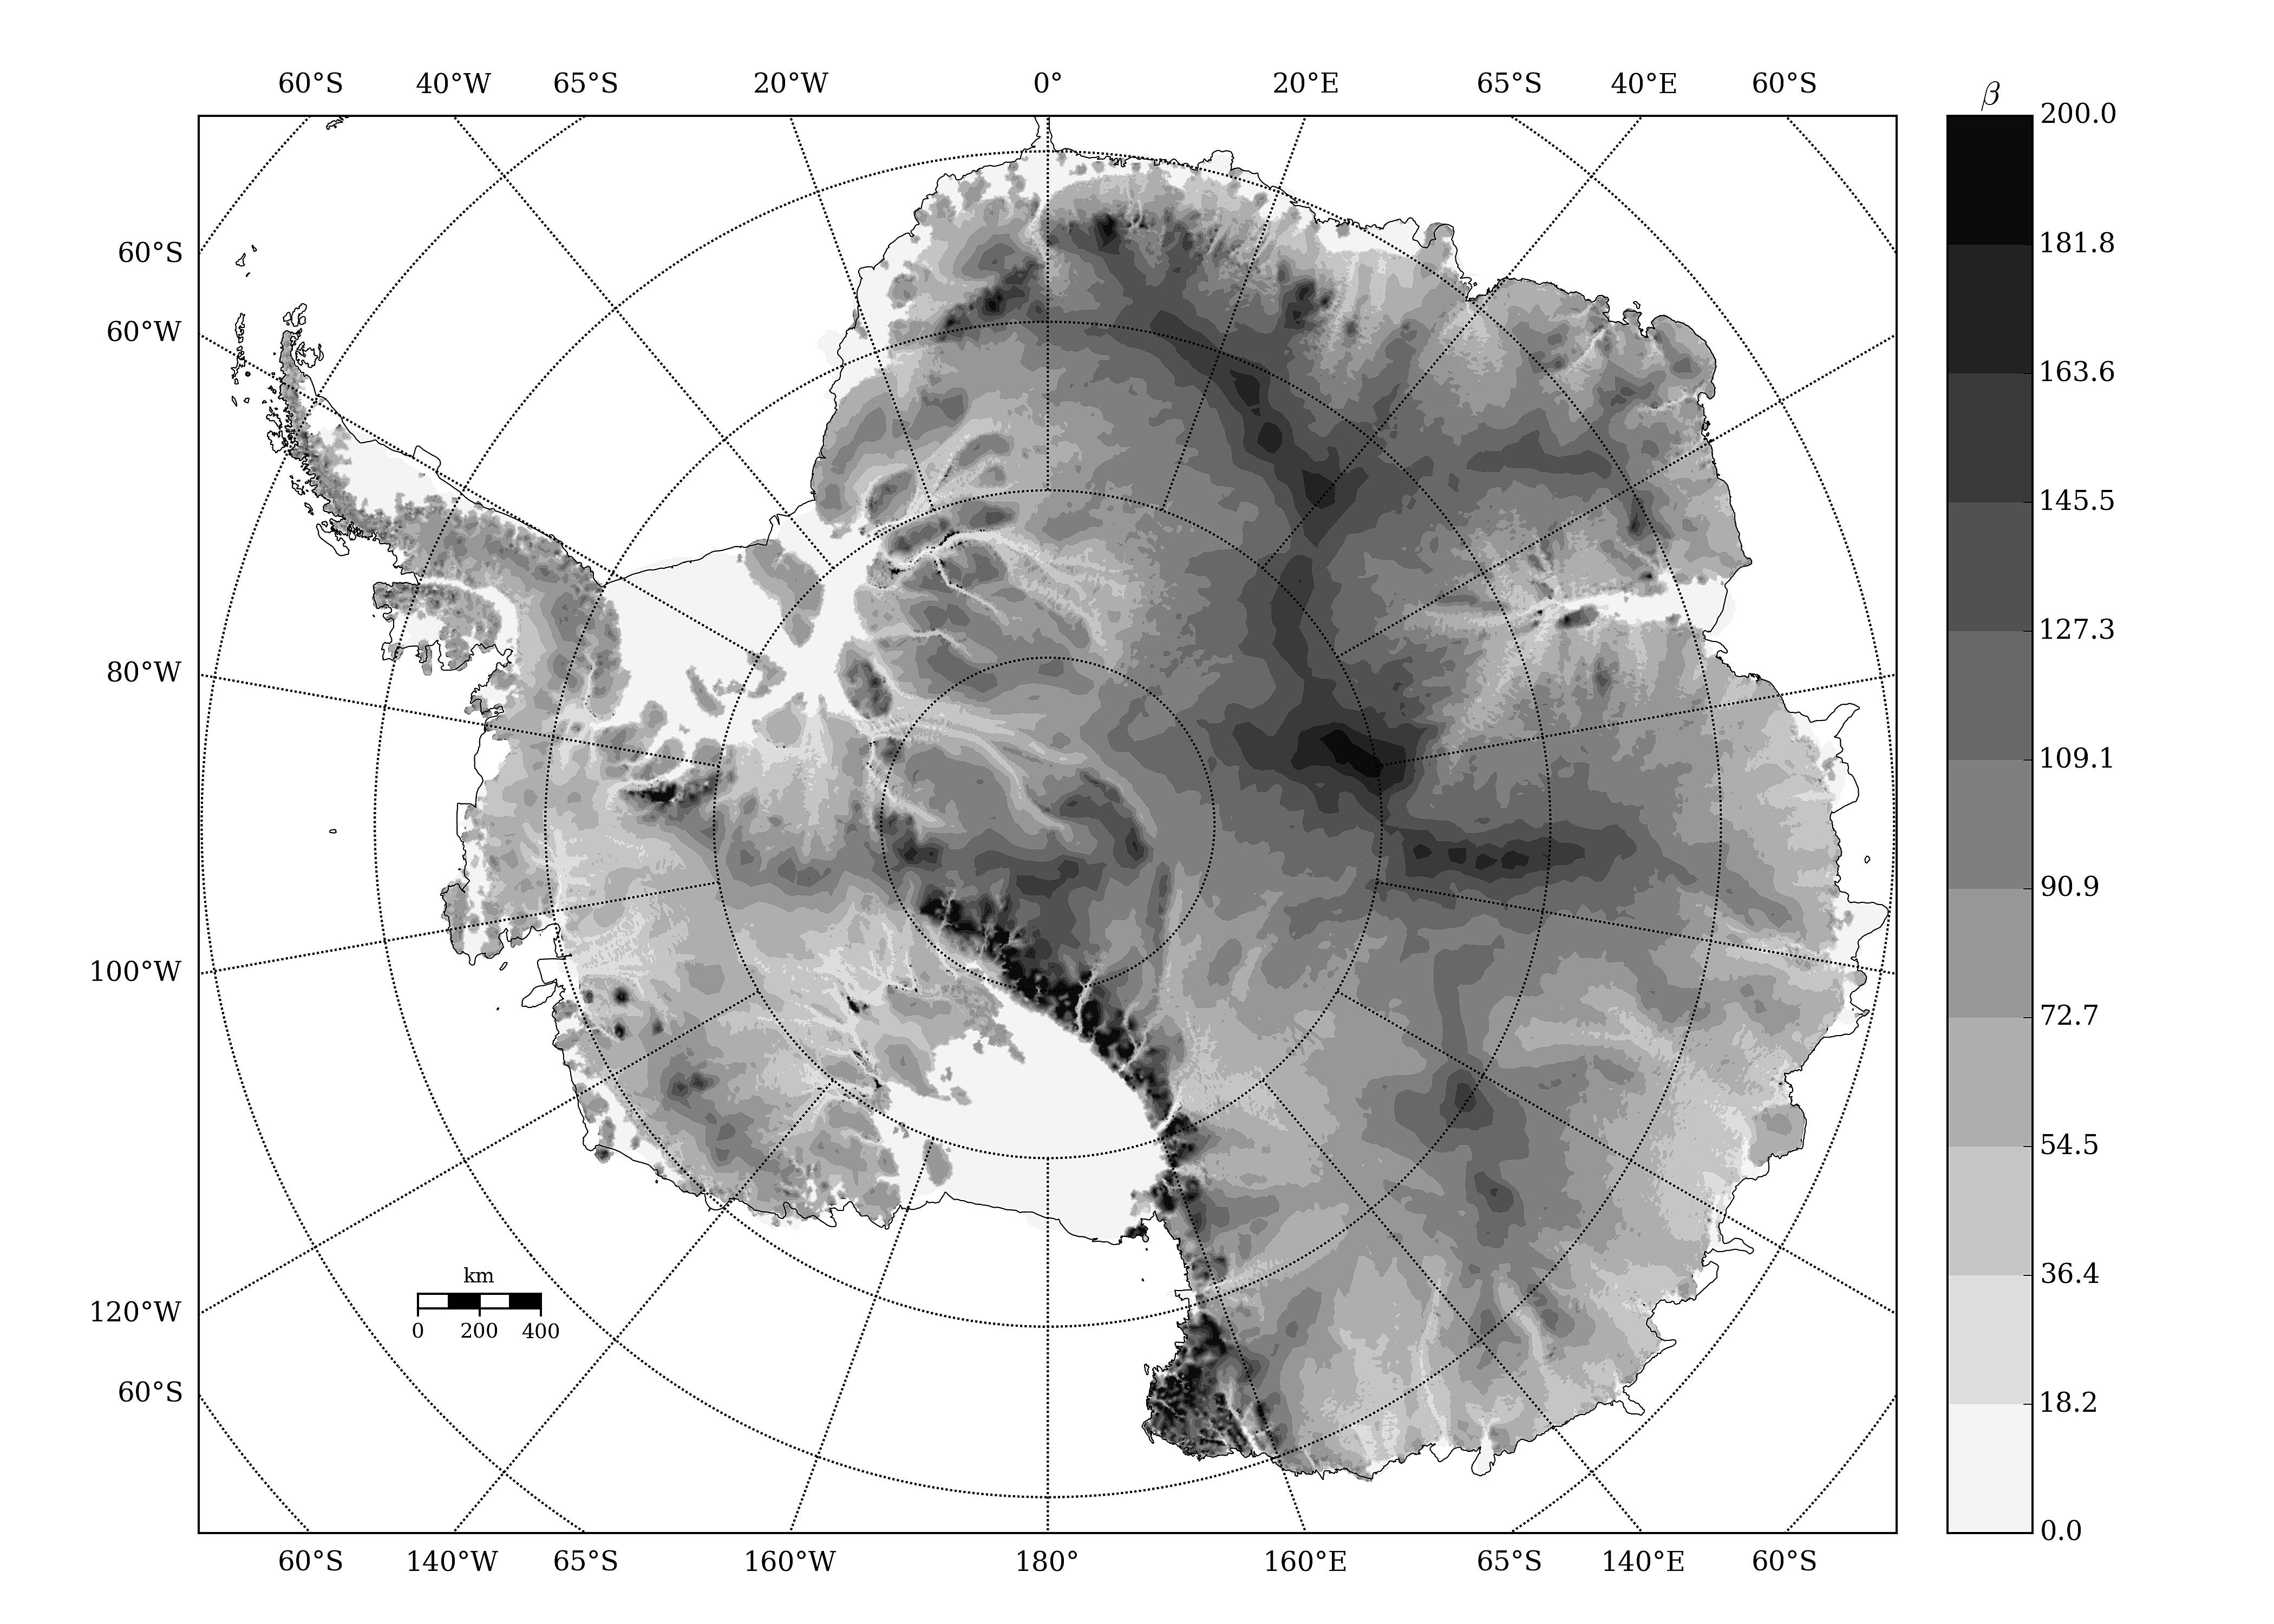
\includegraphics[width=1.0\textwidth]{images/antarctica/stats/GLM_beta_Ubar.jpg}
  \end{minipage}
	\caption[]{GLM-derived basal traction in (Pa a/m)$^{1/2}$ derived with $\mathbf{\bar{u}}$.}
\end{figure}

\begin{figure}
  \centering
  \begin{minipage}[b]{0.47\linewidth}
    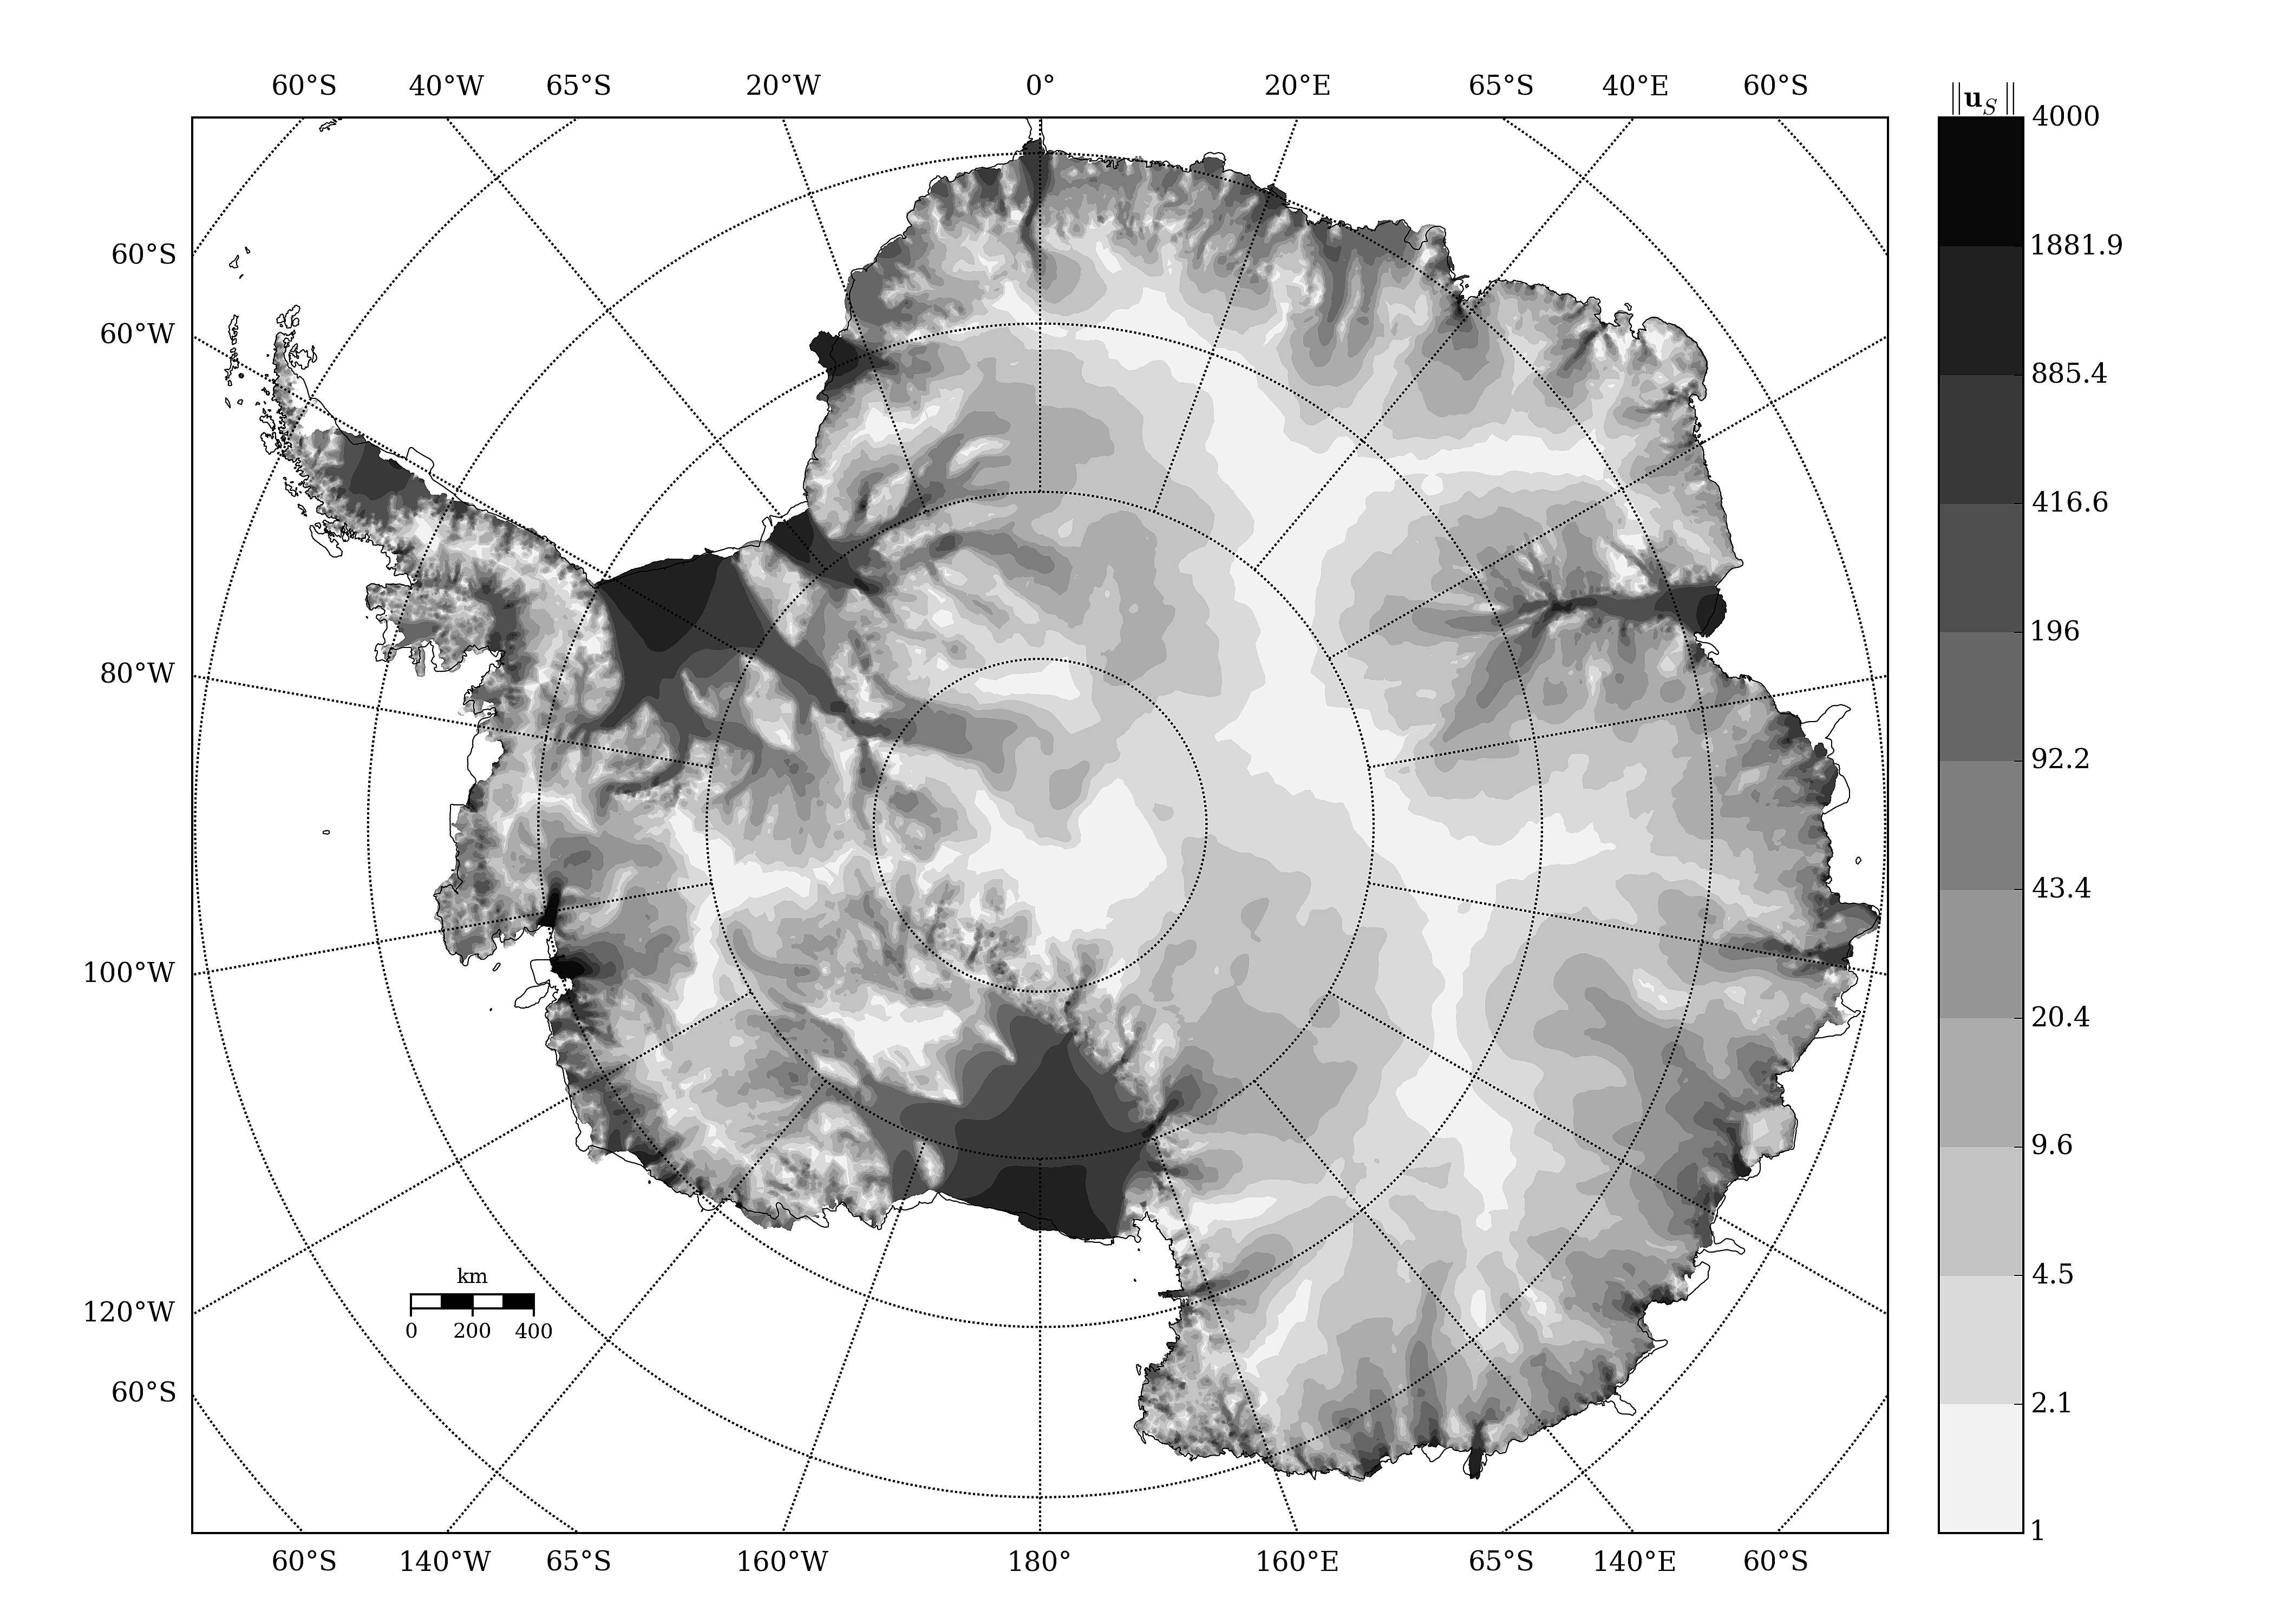
\includegraphics[width=1.0\textwidth]{images/antarctica/stats/GLM_Us_U.jpg}
  \end{minipage}
  \quad
  \begin{minipage}[b]{0.47\linewidth}
    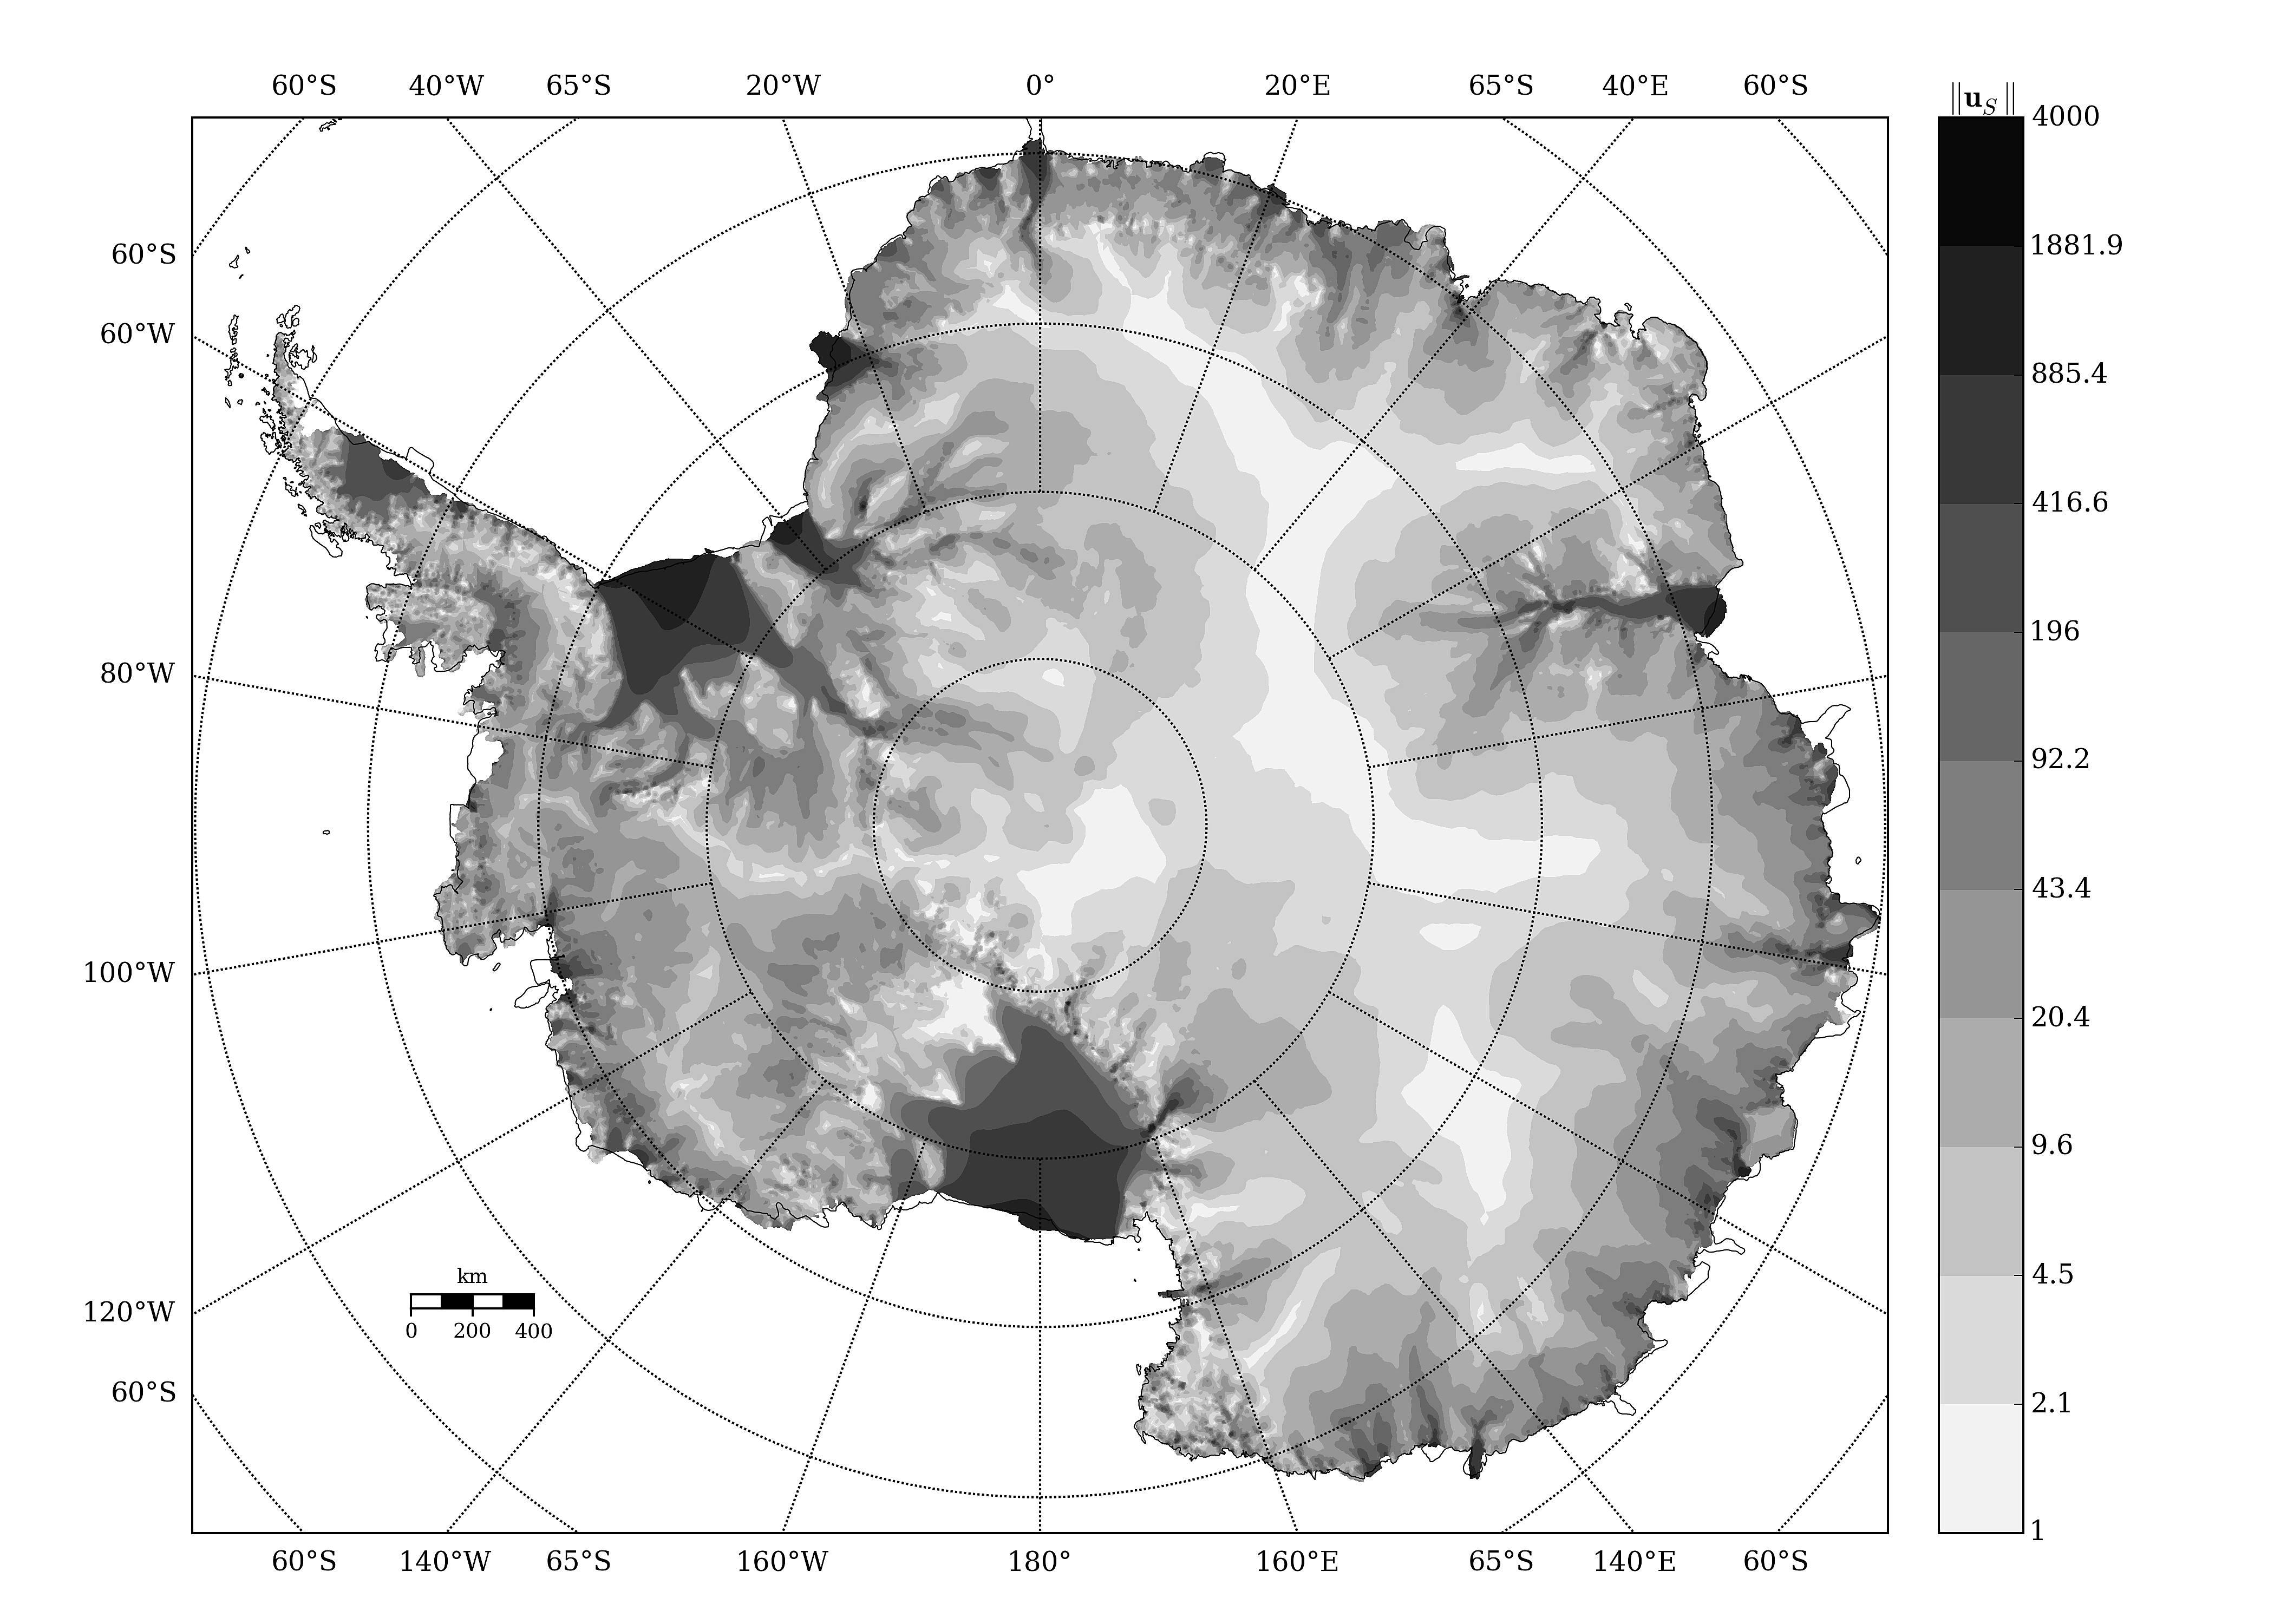
\includegraphics[width=1.0\textwidth]{images/antarctica/stats/GLM_Us_Ubar.jpg}
  \end{minipage}
  \caption[]{Surface speed using GLM-basal-traction derived with $\mathbf{u}_B$ (left) and $\mathbf{\bar{u}}$ (right).}
\end{figure}


% results ====================================================================
\section{Dynamic simulation}

As a final test, we perform a dynamic run beginning with no ice that utilizes climate forcings from the EISMINT experiment \citep{payne_2000}.  For this admittedly simple test, we apply the statistical model over an 800 km radius of bed topography located adjacent to the Amery Ice Shelf, chosen for its deep trench and widely-varying topography, and was performed with a simplified vertically-integrated 2D model.  The results are presented below.

\begin{figure}
  \centering
  
  \begin{minipage}[b]{0.30\linewidth}
    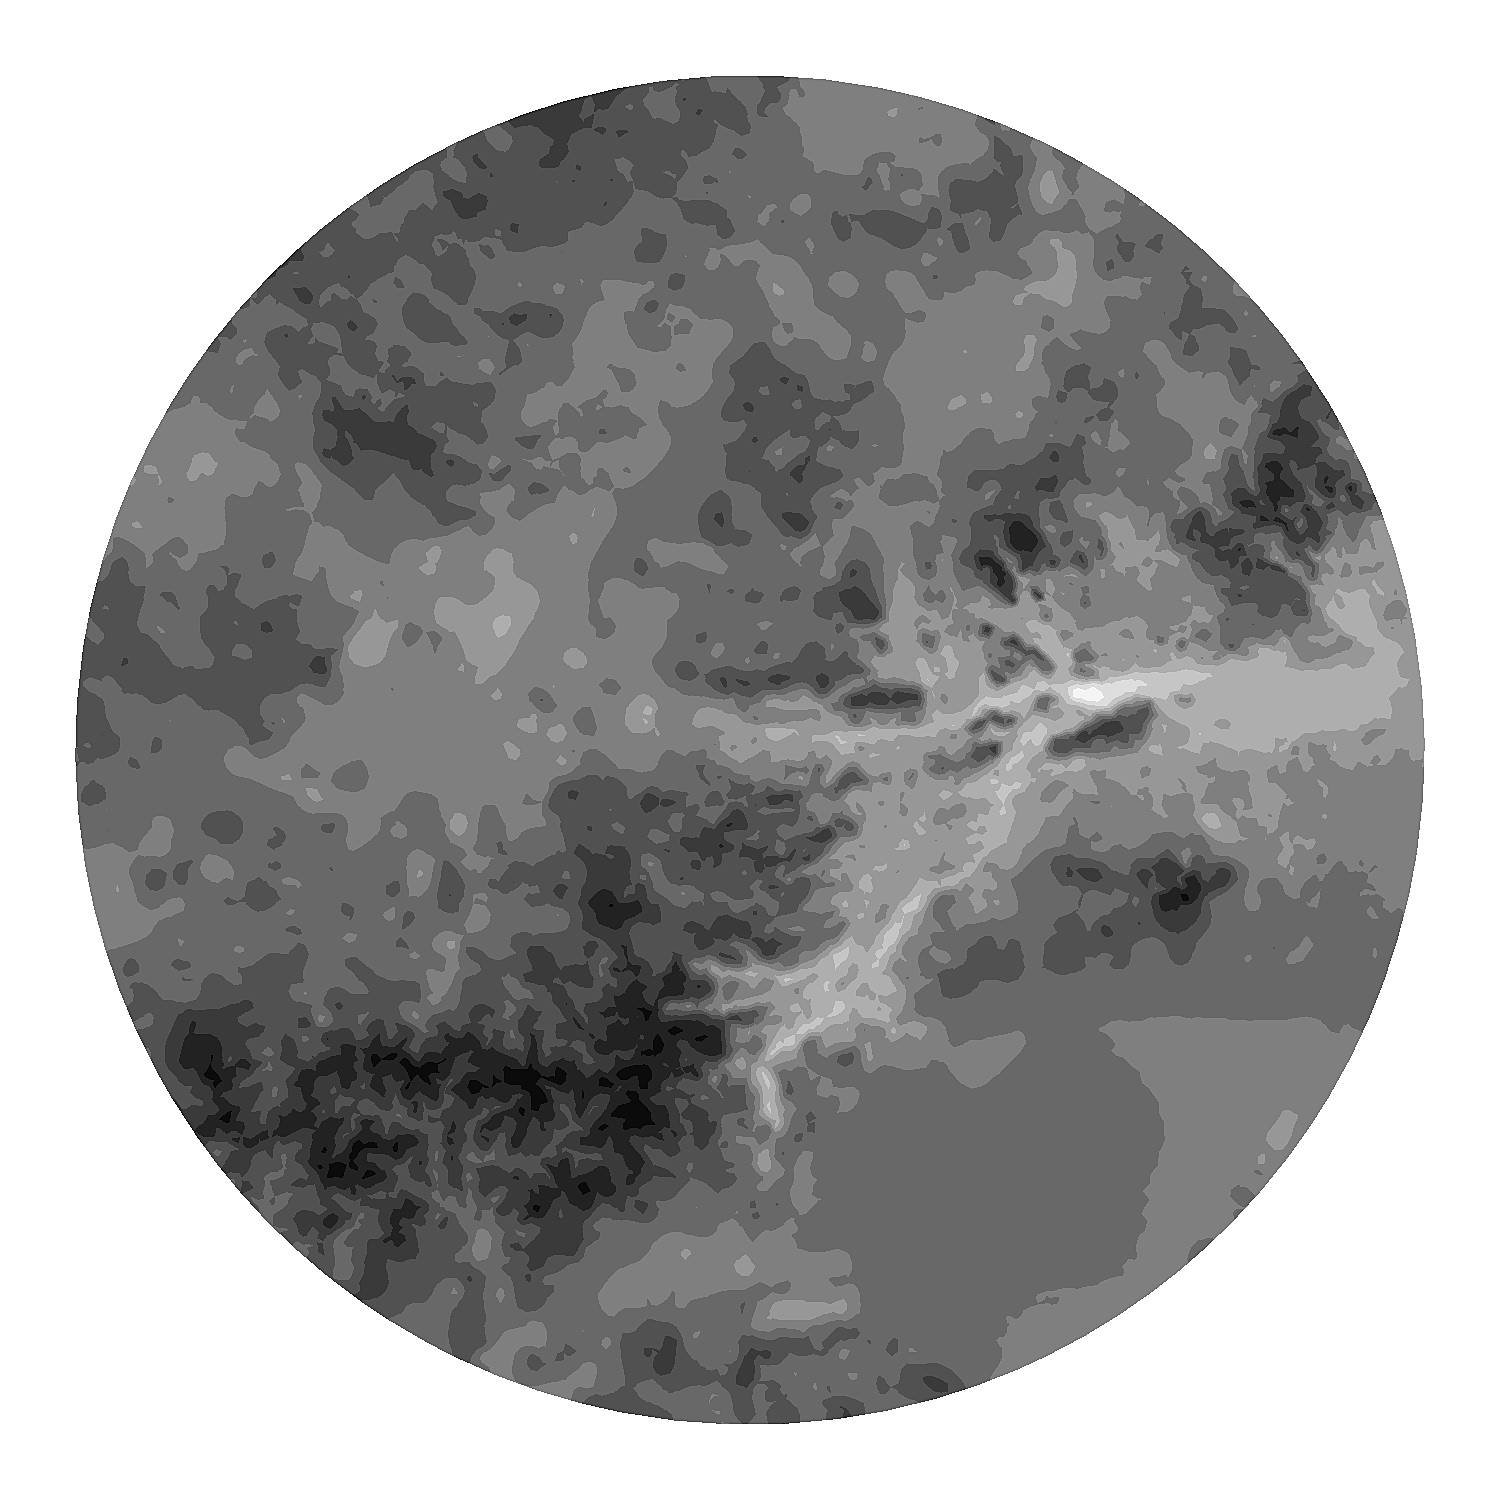
\includegraphics[width=1.0\textwidth]{images/EISMINT_II/vars/B.jpg}
  \end{minipage}
  \quad
  \begin{minipage}[b]{0.30\linewidth}
    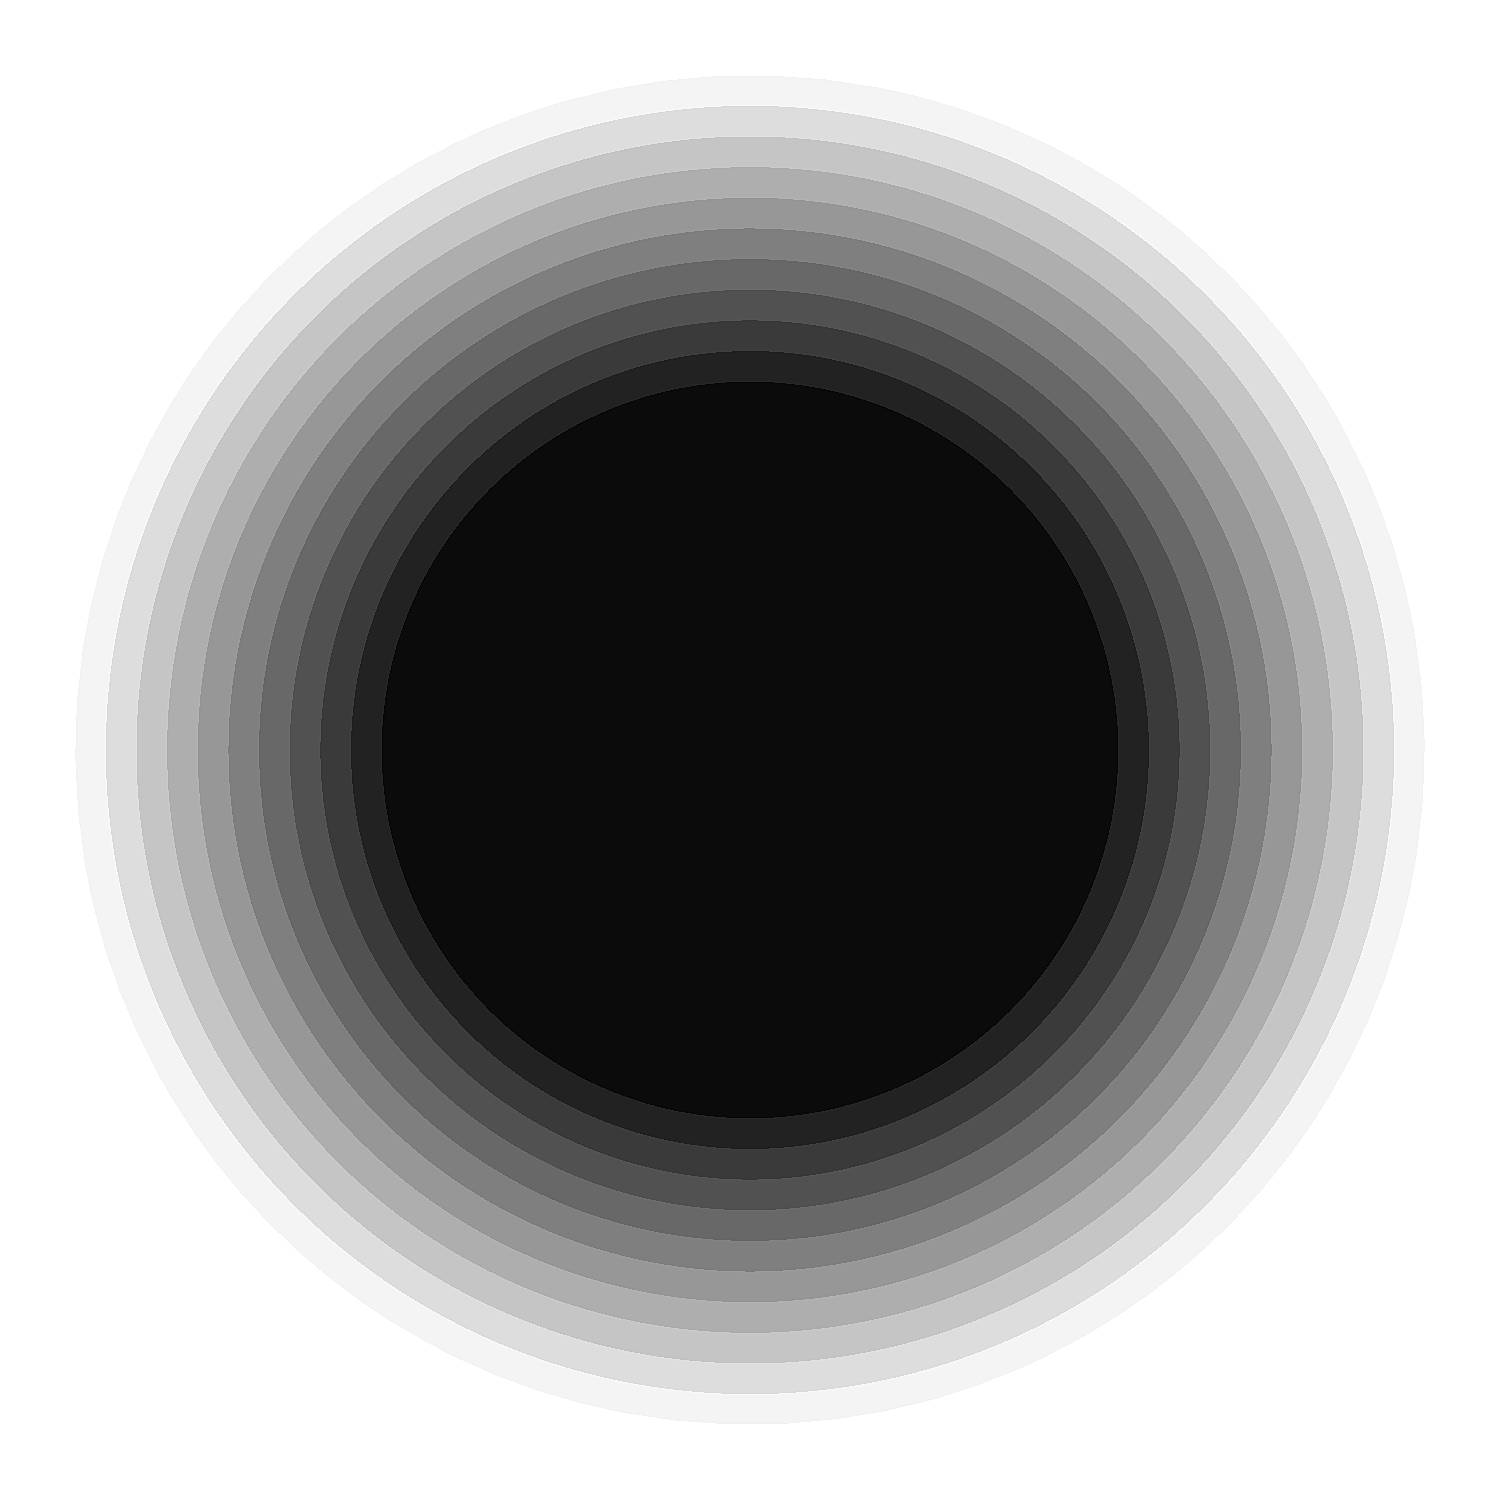
\includegraphics[width=1.0\textwidth]{images/EISMINT_II/vars/adot.jpg}
  \end{minipage}
  \quad
  \begin{minipage}[b]{0.30\linewidth}
    
\includegraphics[width=1.0\textwidth]{images/EISMINT_II/vars/T_s.jpg}
  \end{minipage}
  
  \begin{minipage}[b]{0.30\linewidth}
    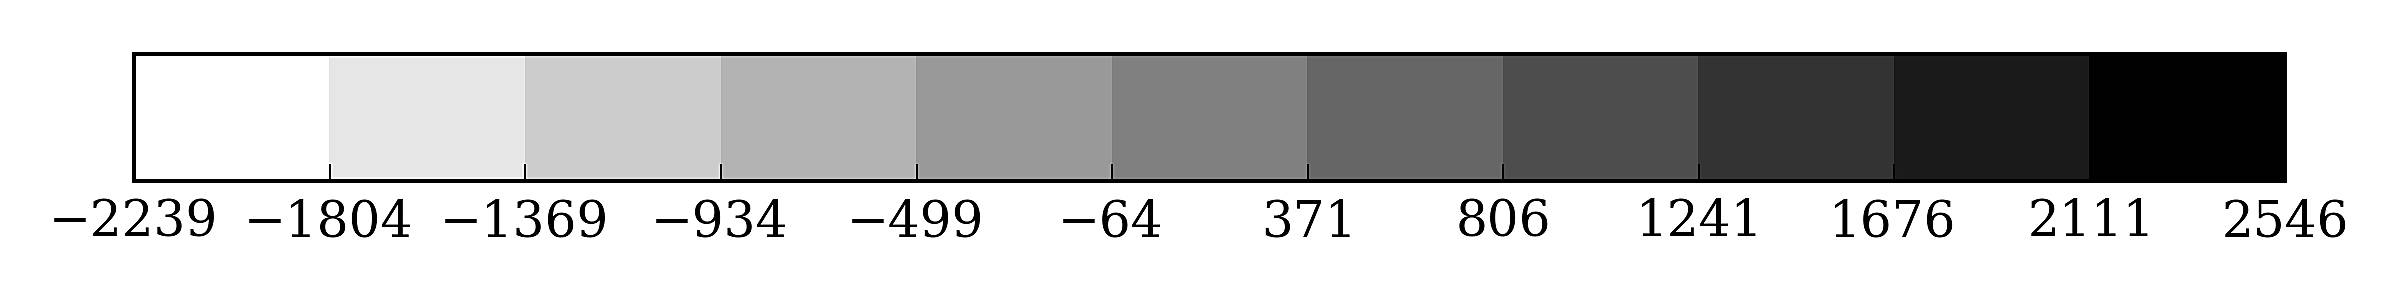
\includegraphics[width=1.0\textwidth]{images/EISMINT_II/vars/B_cb.jpg}
  \end{minipage}
  \quad
  \begin{minipage}[b]{0.30\linewidth}
    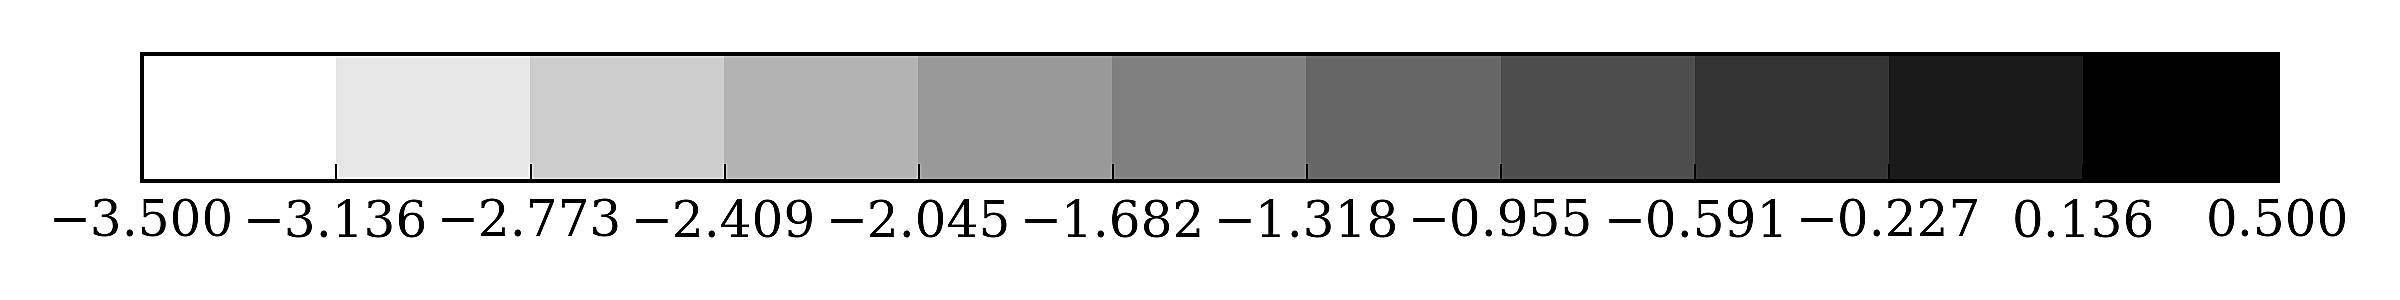
\includegraphics[width=1.0\textwidth]{images/EISMINT_II/vars/adot_cb.jpg}
  \end{minipage}
  \quad
  \begin{minipage}[b]{0.30\linewidth}
    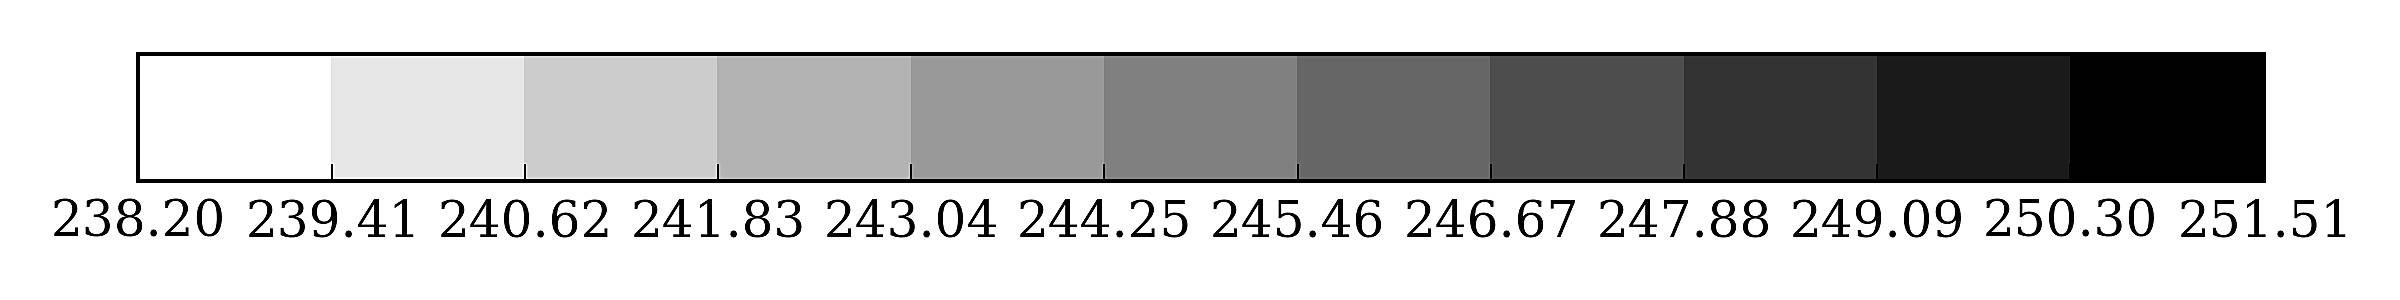
\includegraphics[width=1.0\textwidth]{images/EISMINT_II/vars/T_s_cb.jpg}
  \end{minipage}
  \caption[]{Bed height in meters (left), \ie meters per annum accumulation/ablation rate $\dot{a}$ (middle), and surface temperature in $^\circ$C (right) used as inputs for the experiment.}
\end{figure}


\begin{figure}
  \centering
  
  \begin{minipage}[b]{0.30\linewidth}
    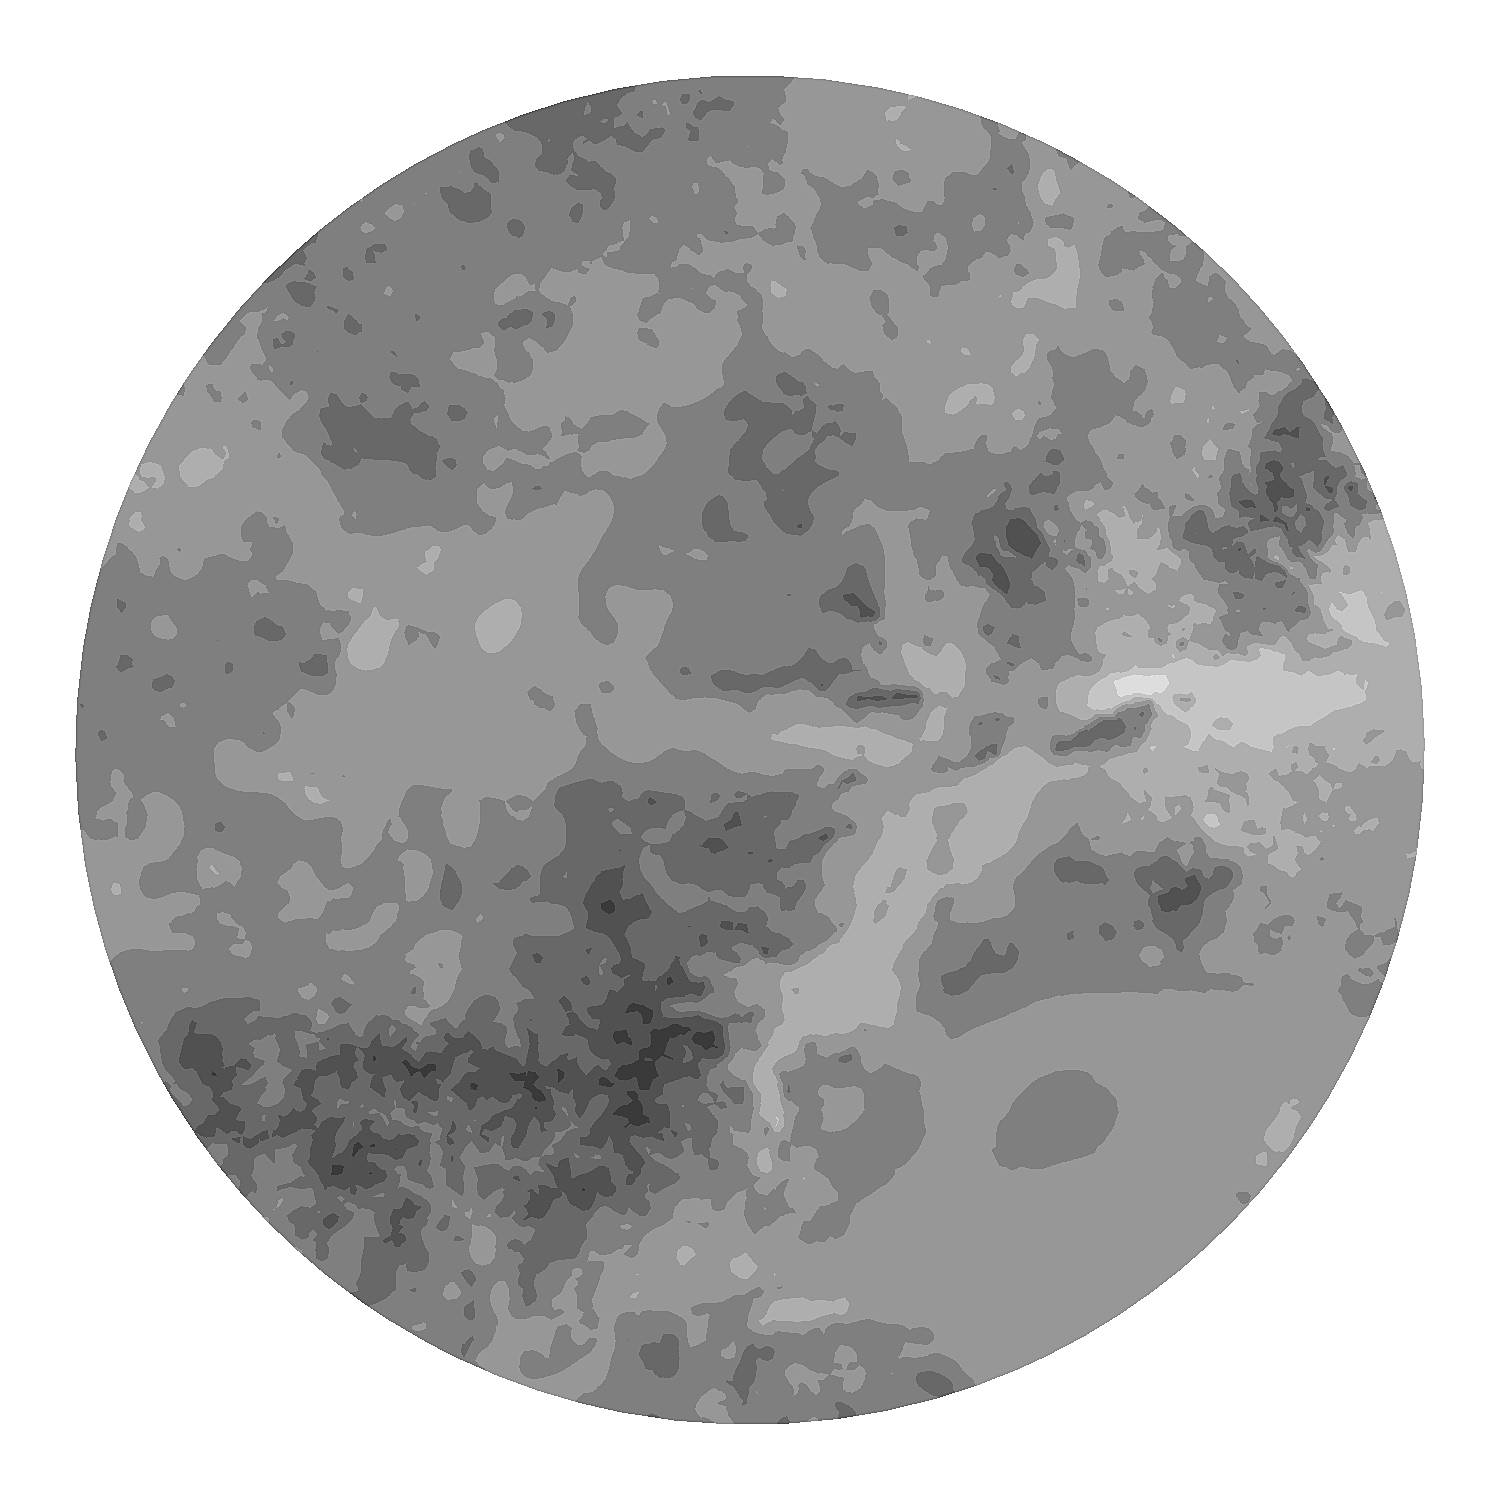
\includegraphics[width=1.0\textwidth]{images/EISMINT_II/U/S_500.jpg}
  \end{minipage}
  \quad
  \begin{minipage}[b]{0.30\linewidth}
    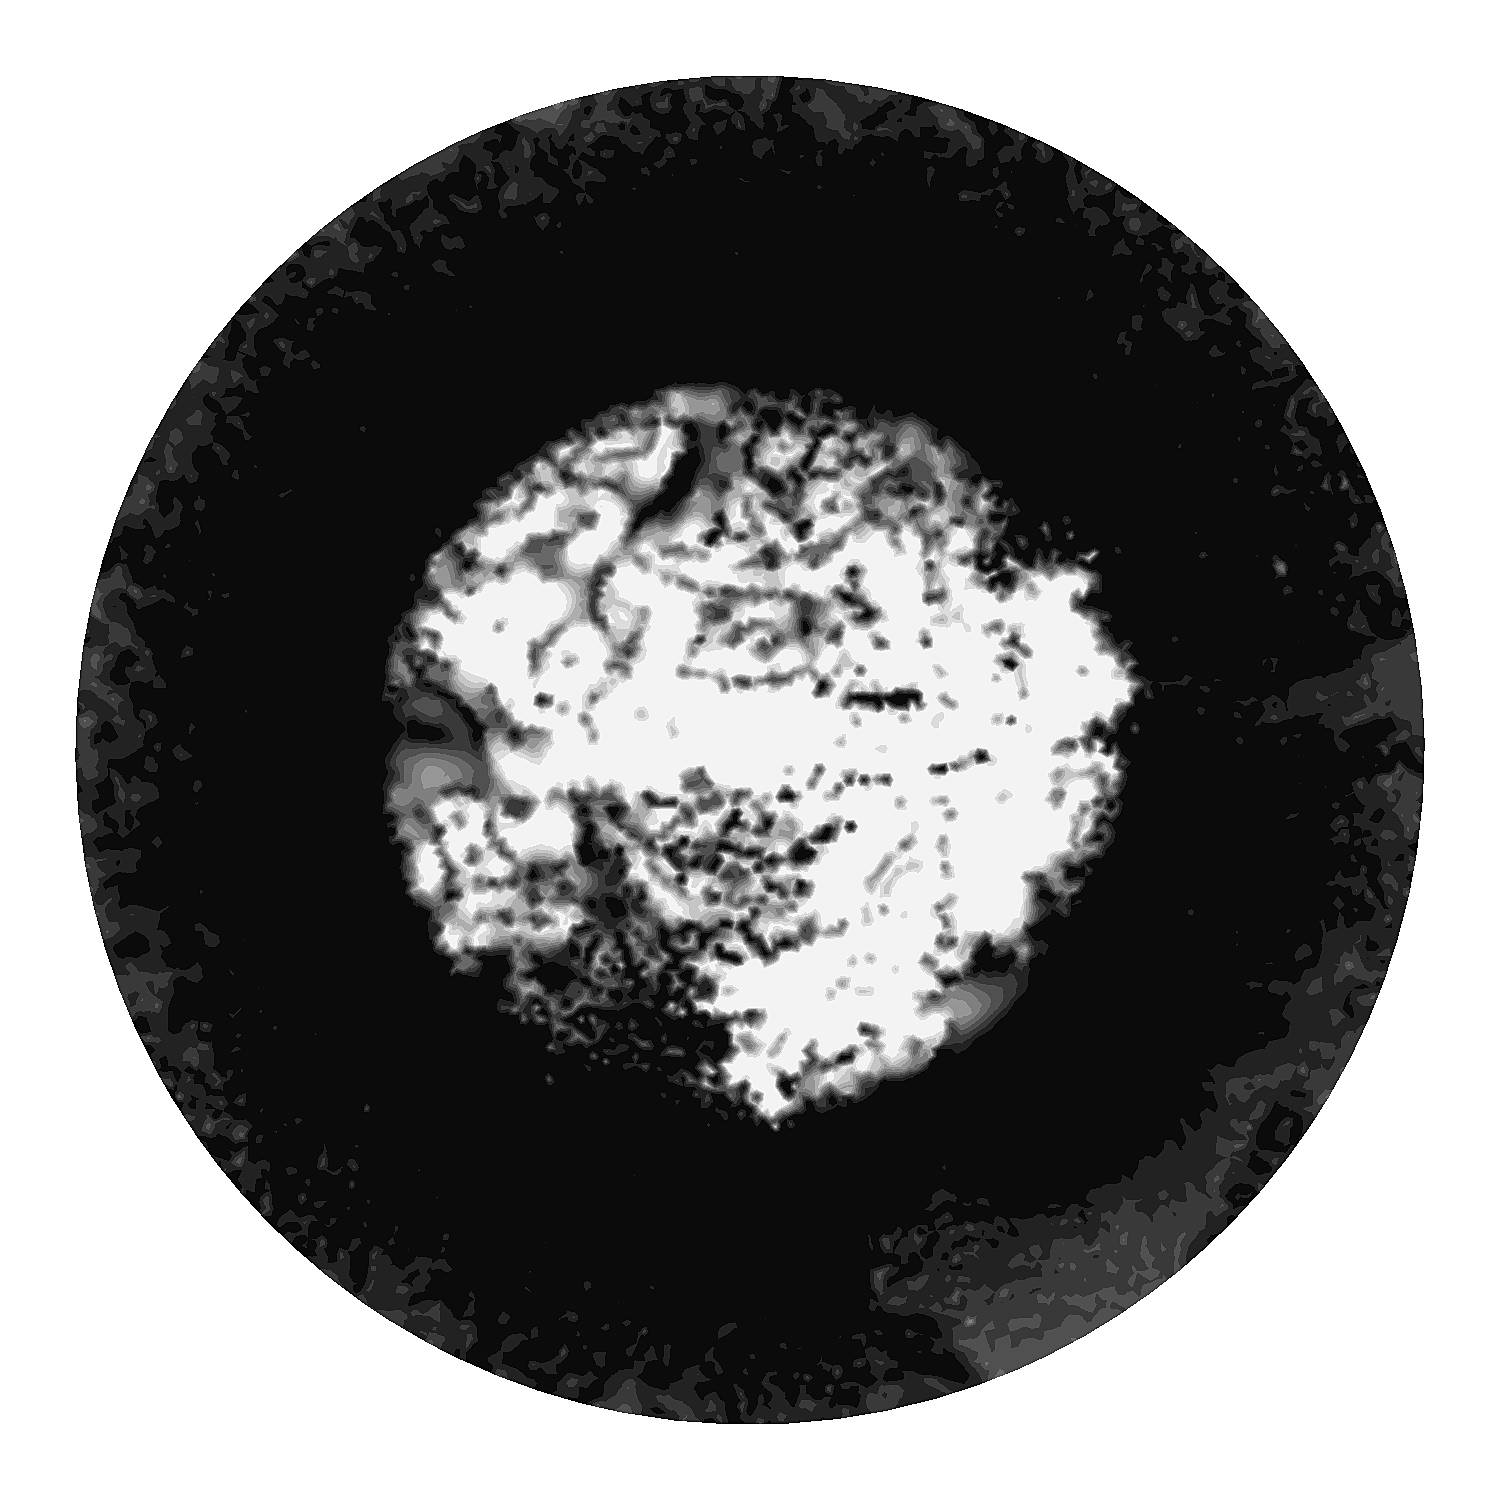
\includegraphics[width=1.0\textwidth]{images/EISMINT_II/U/beta_500.jpg}
  \end{minipage}
  \quad
  \begin{minipage}[b]{0.30\linewidth}
    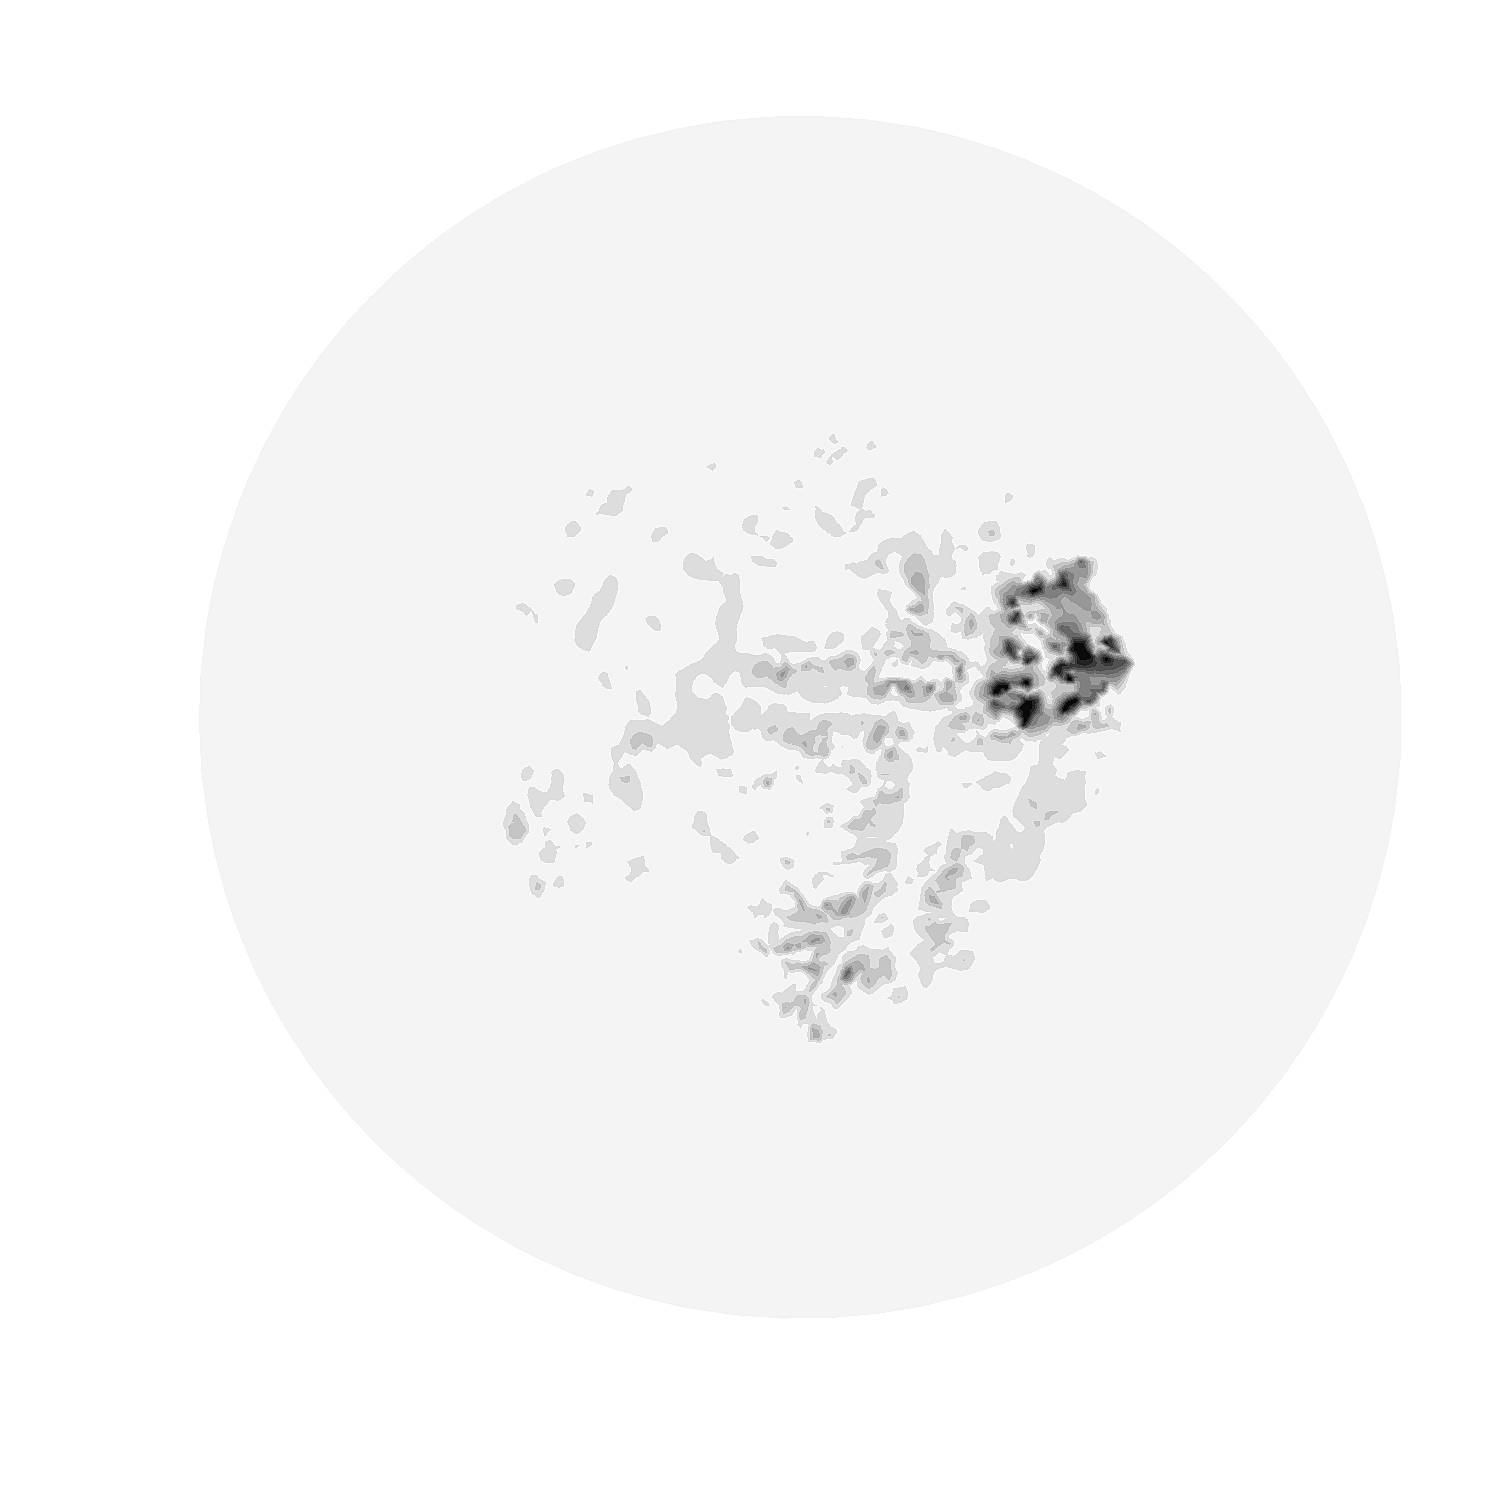
\includegraphics[width=1.0\textwidth]{images/EISMINT_II/U/U_mag_500.jpg}
  \end{minipage}
  
  \begin{minipage}[b]{0.30\linewidth}
    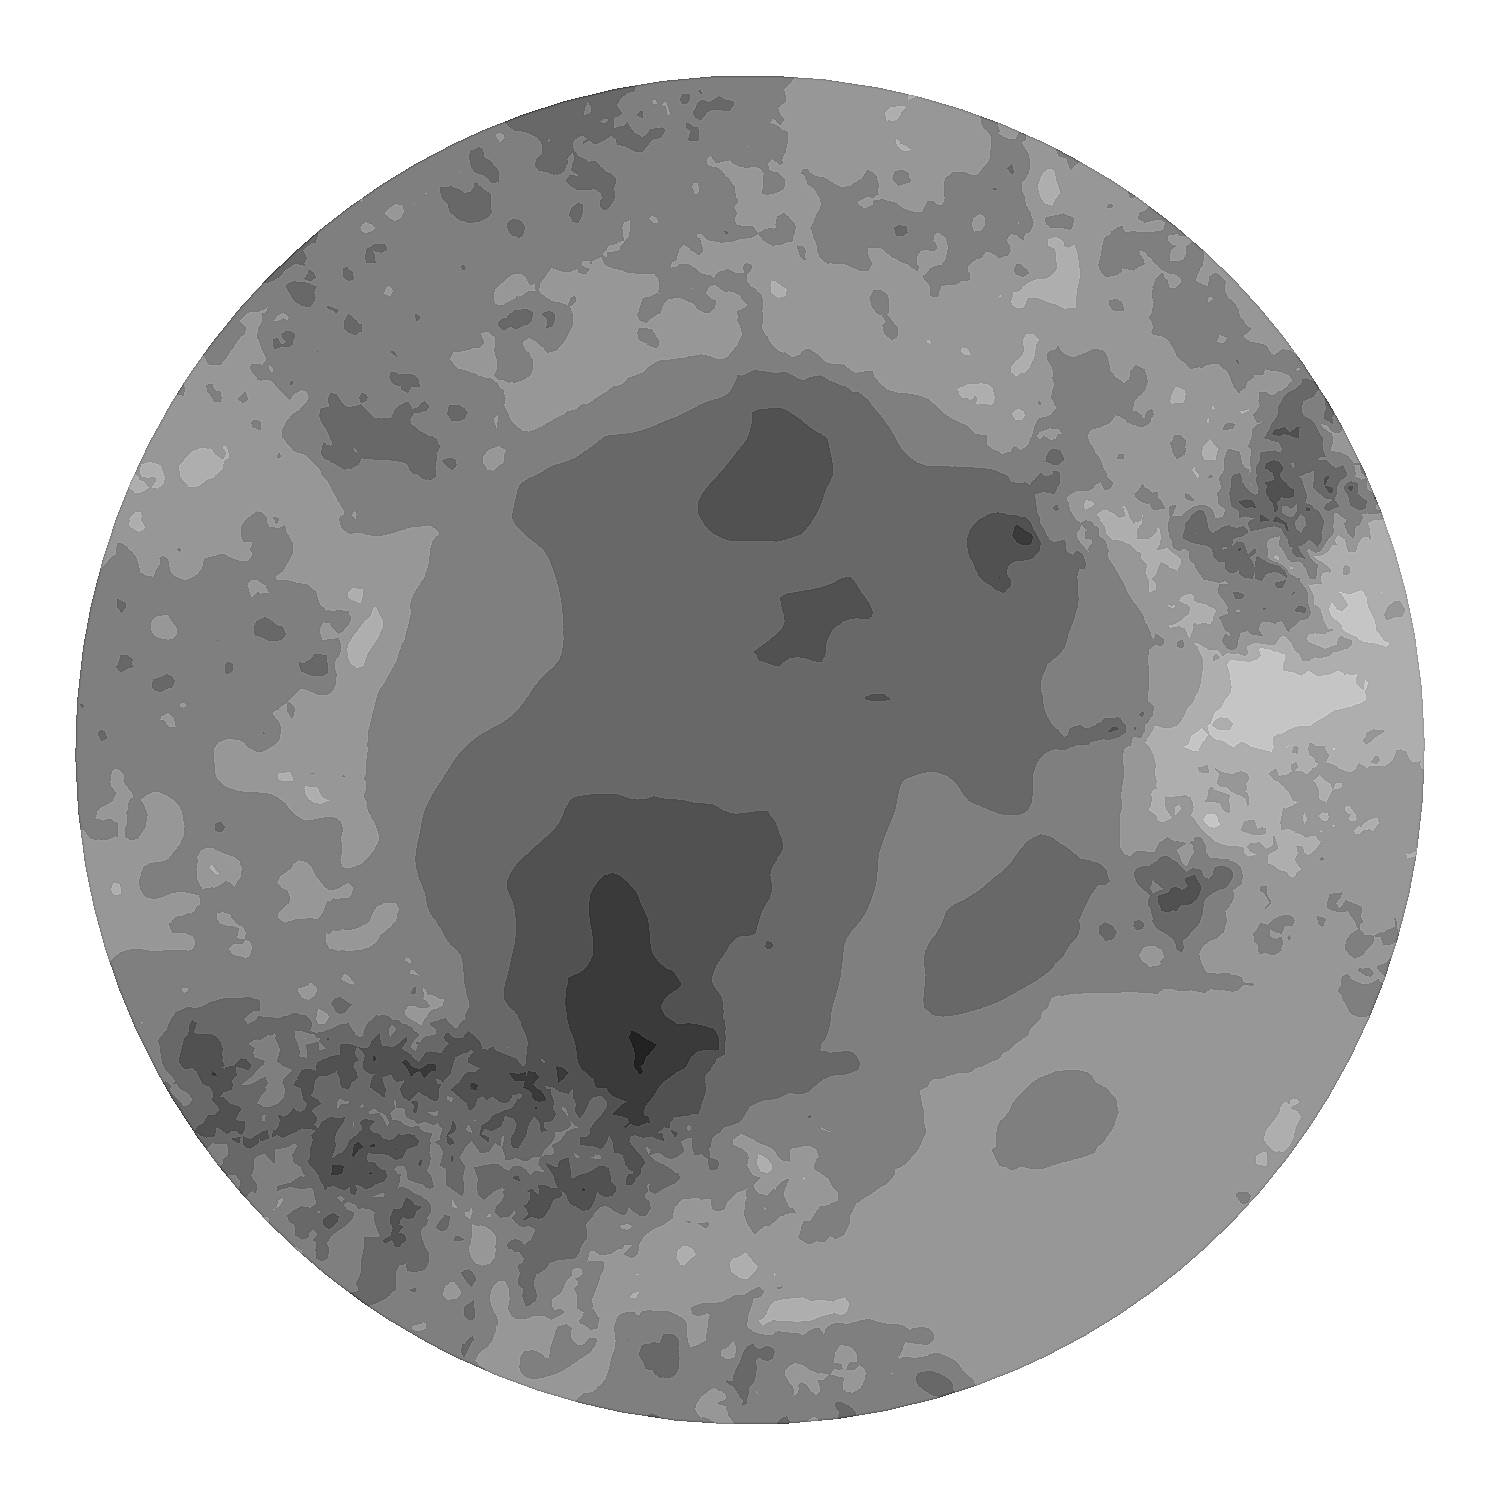
\includegraphics[width=1.0\textwidth]{images/EISMINT_II/U/S_2000.jpg}
  \end{minipage}
  \quad
  \begin{minipage}[b]{0.30\linewidth}
    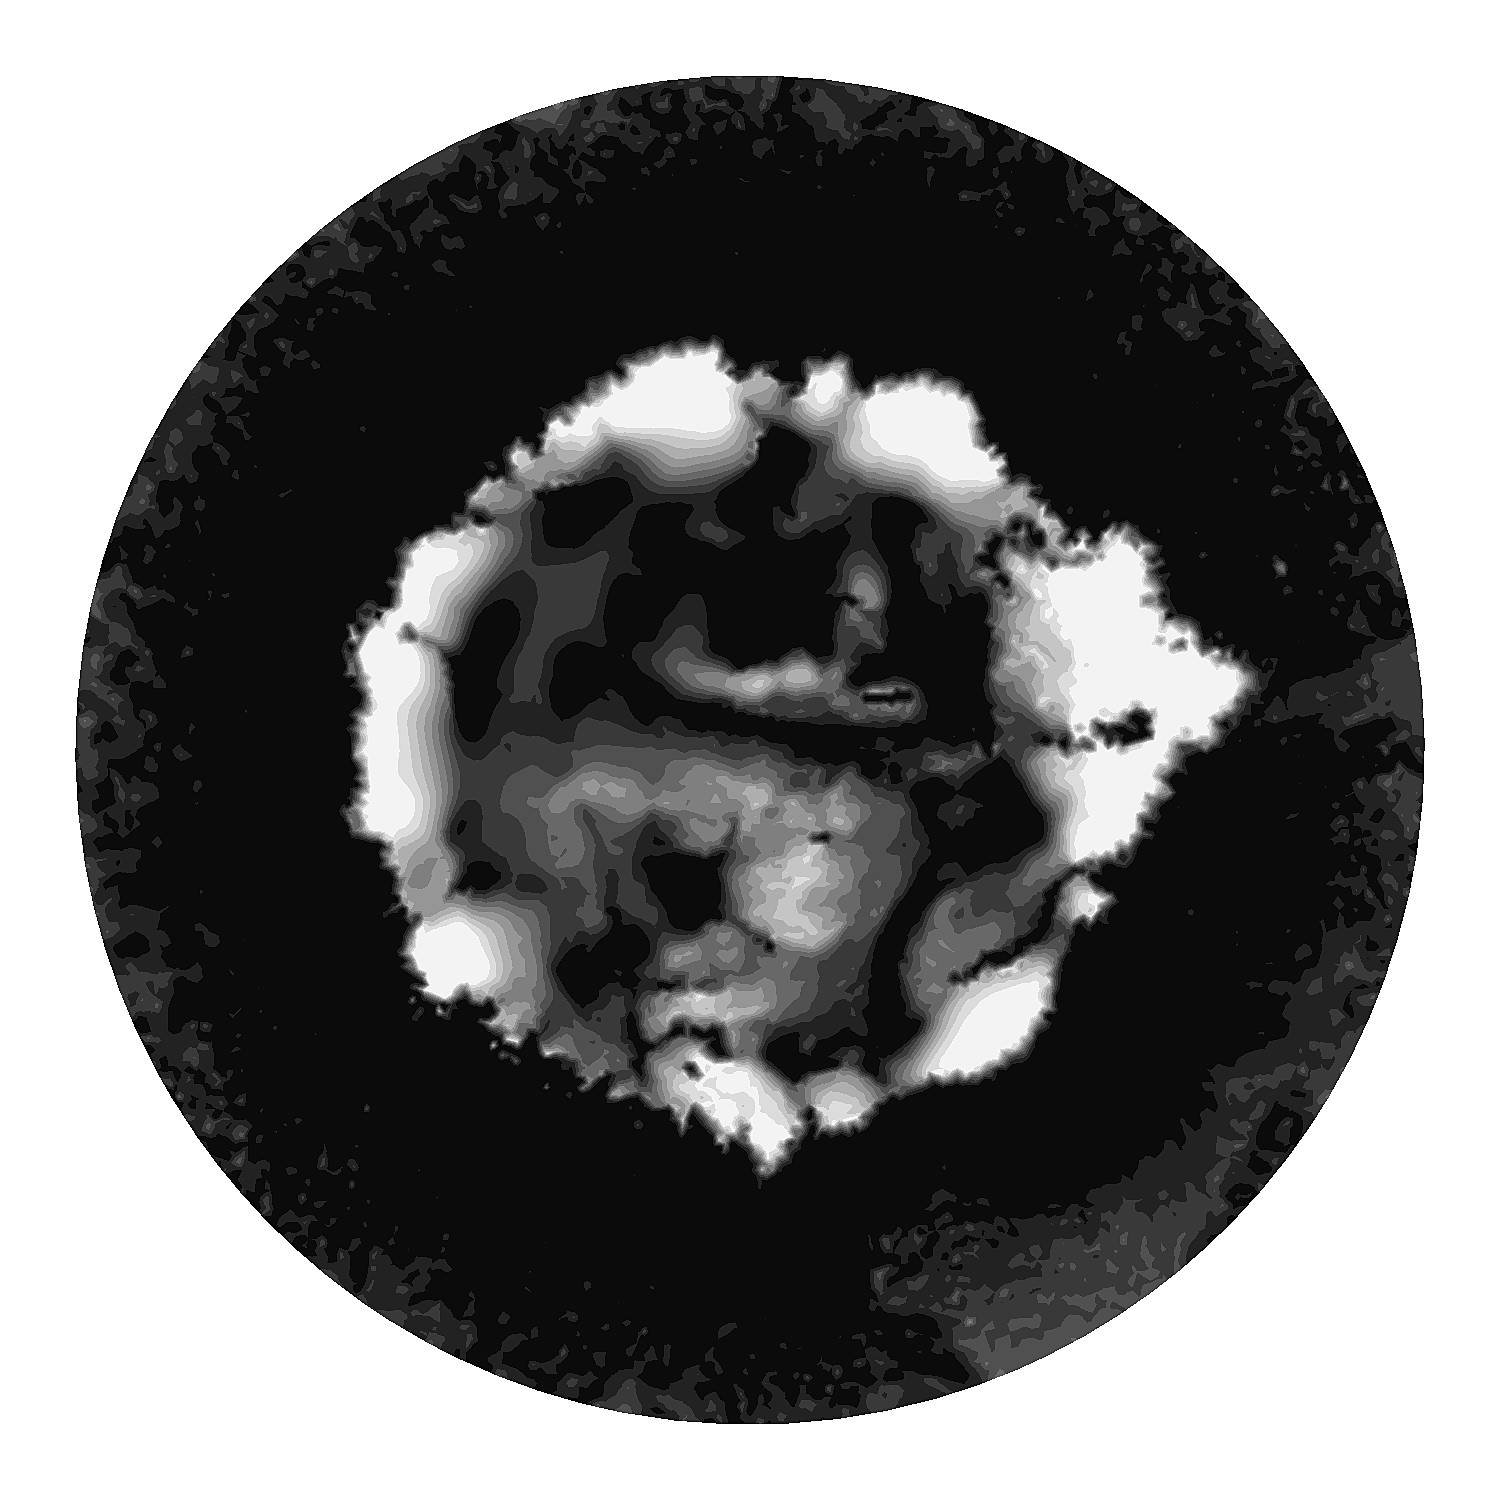
\includegraphics[width=1.0\textwidth]{images/EISMINT_II/U/beta_2000.jpg}
  \end{minipage}
  \quad
  \begin{minipage}[b]{0.30\linewidth}
    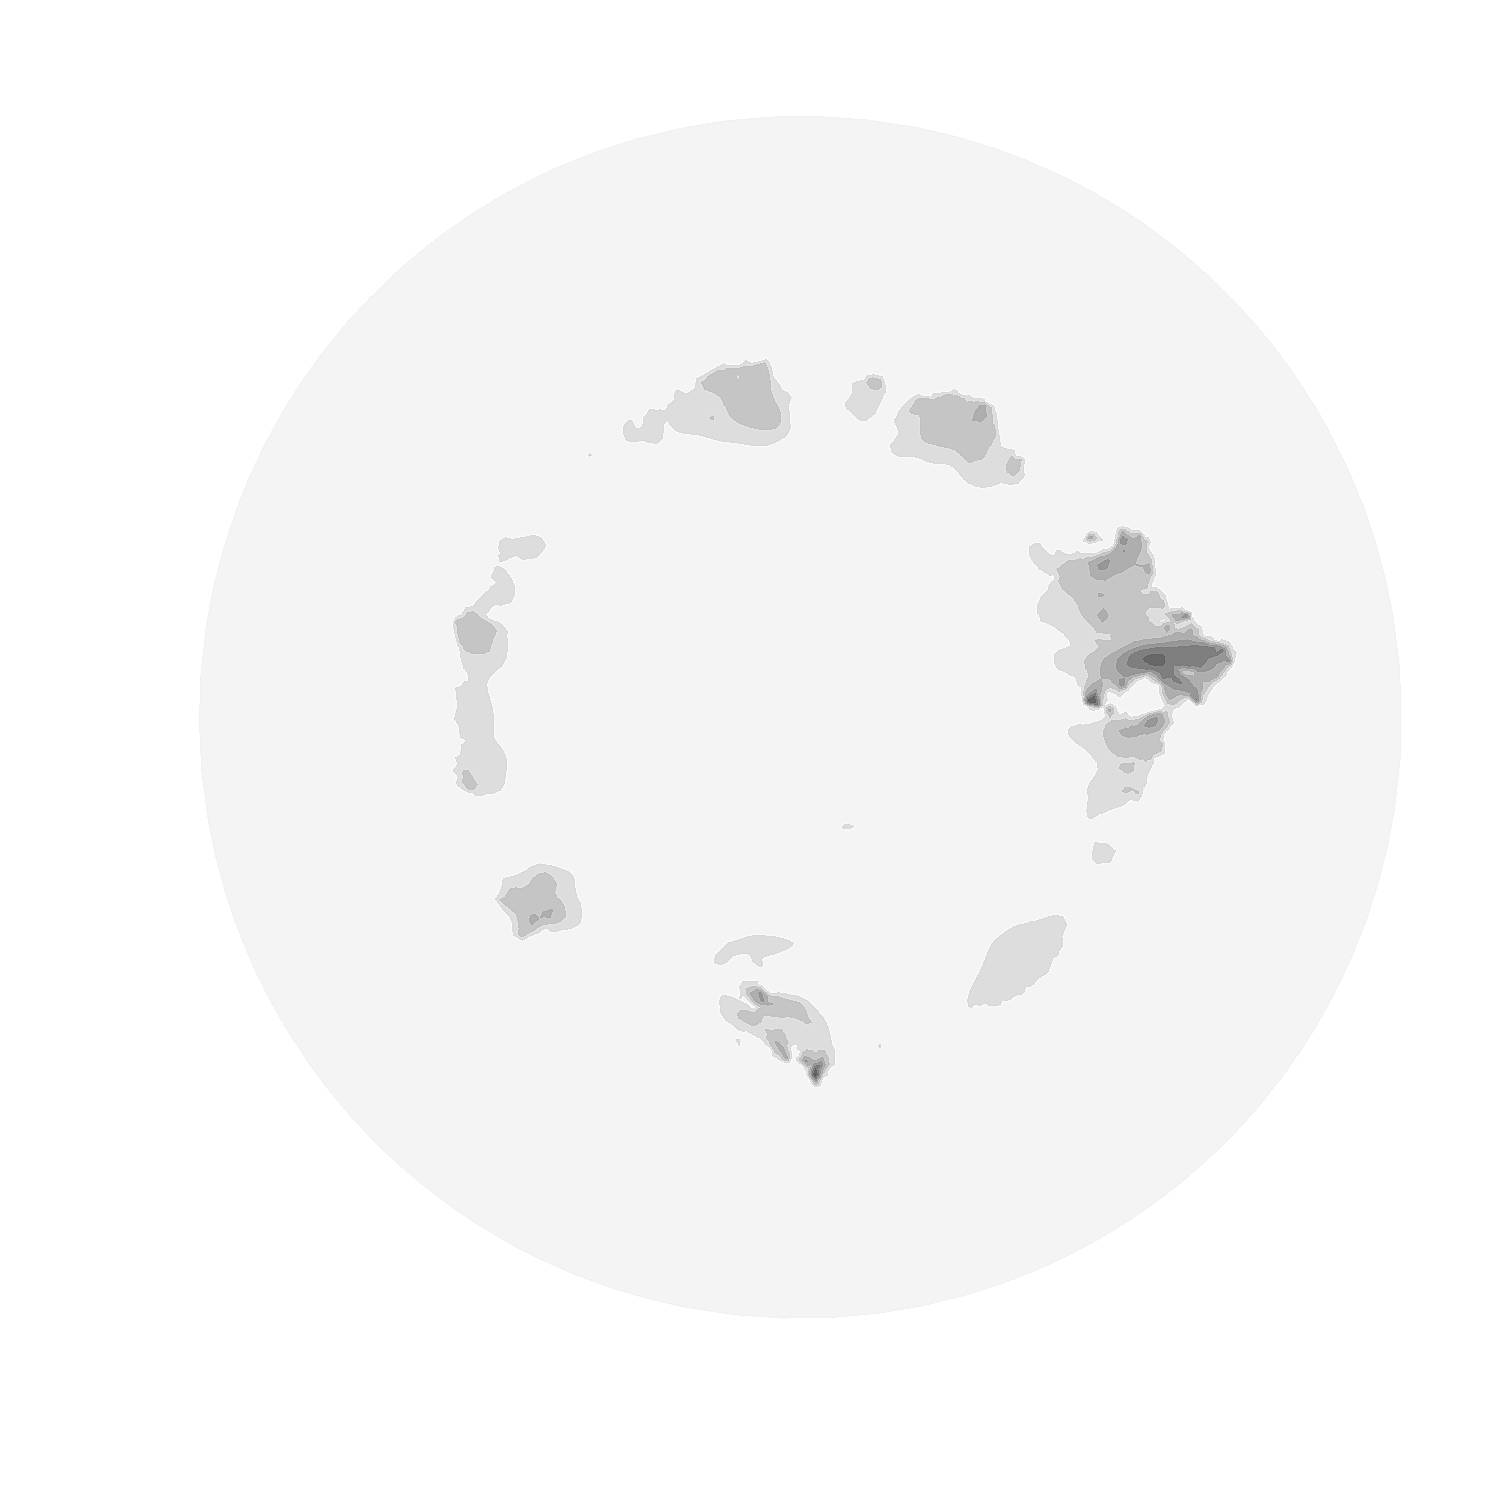
\includegraphics[width=1.0\textwidth]{images/EISMINT_II/U/U_mag_2000.jpg}
  \end{minipage}
  
  \begin{minipage}[b]{0.30\linewidth}
    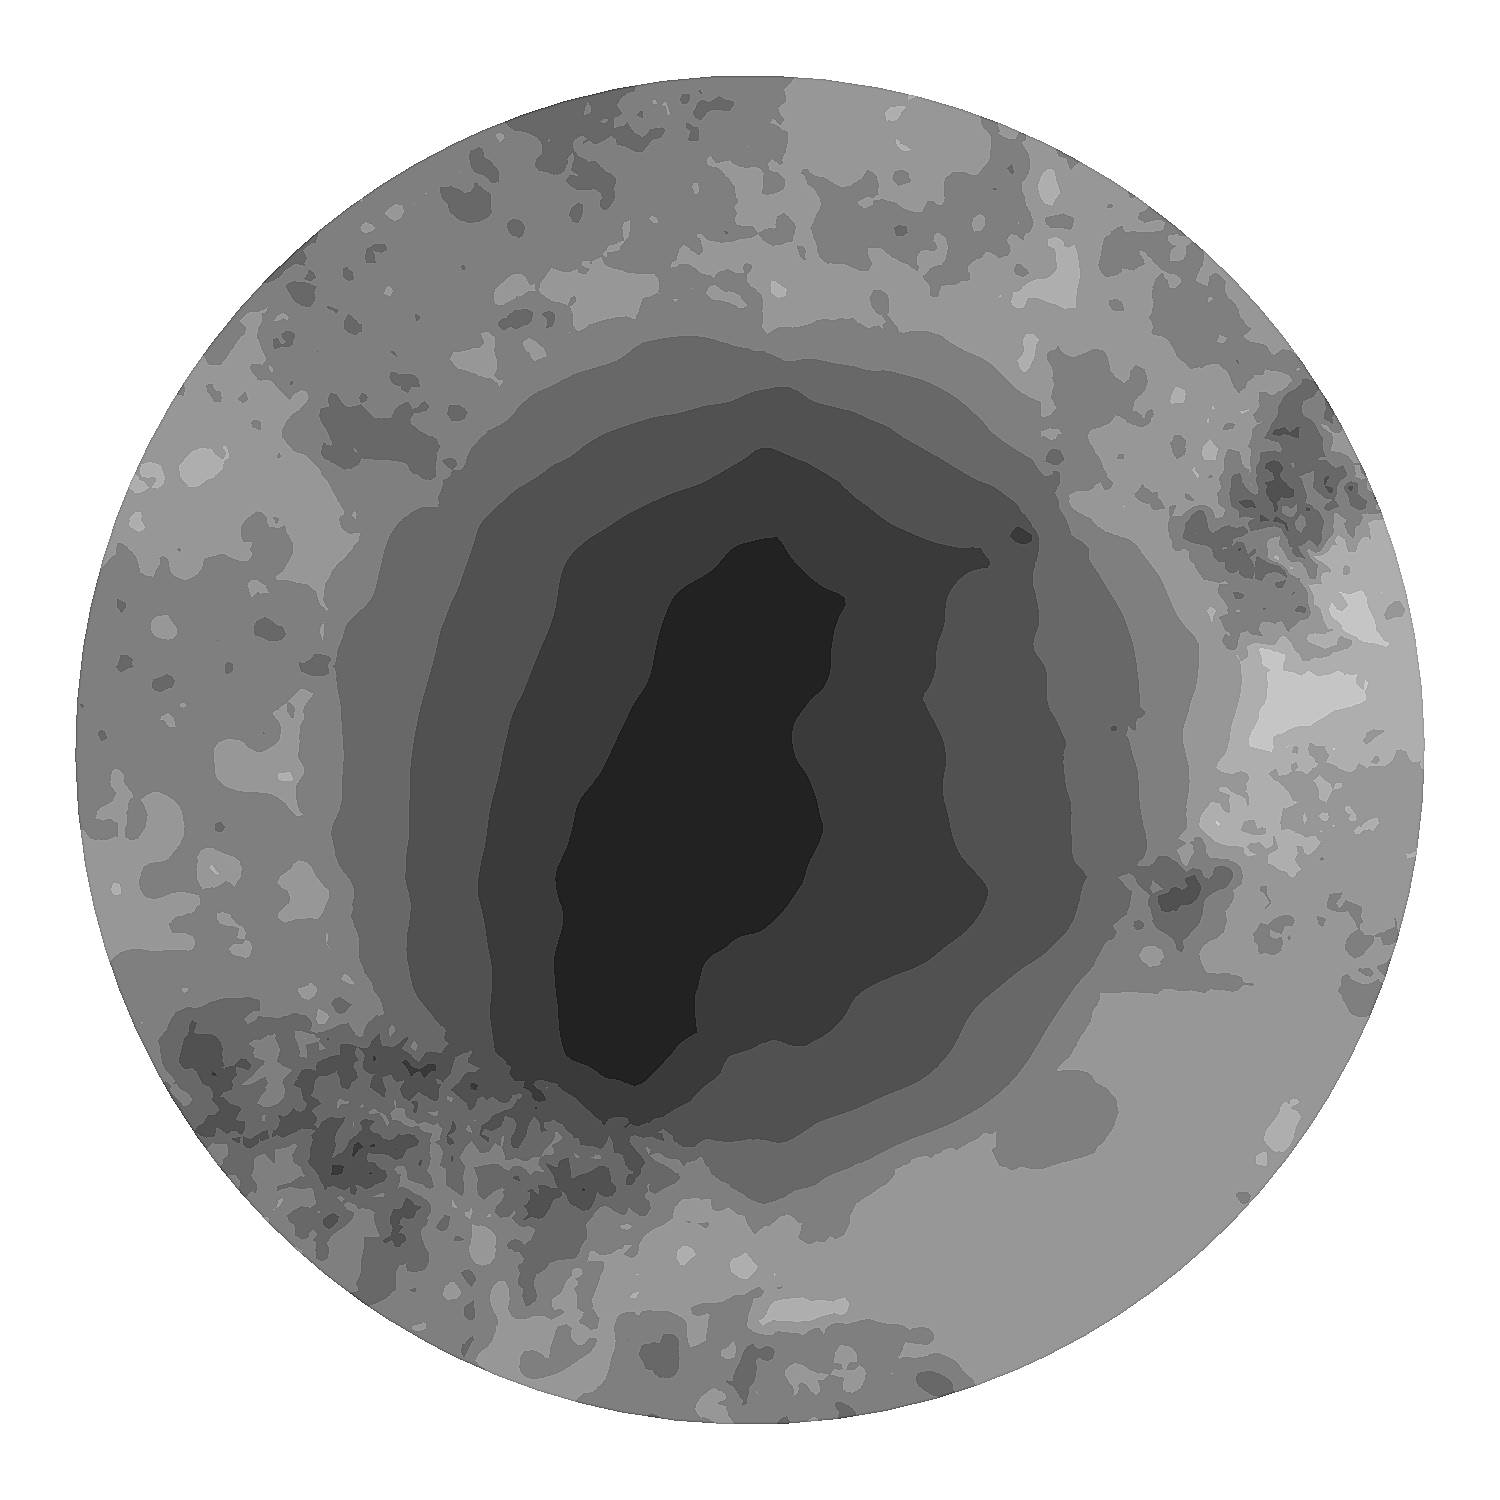
\includegraphics[width=1.0\textwidth]{images/EISMINT_II/U/S_5000.jpg}
  \end{minipage}
  \quad
  \begin{minipage}[b]{0.30\linewidth}
    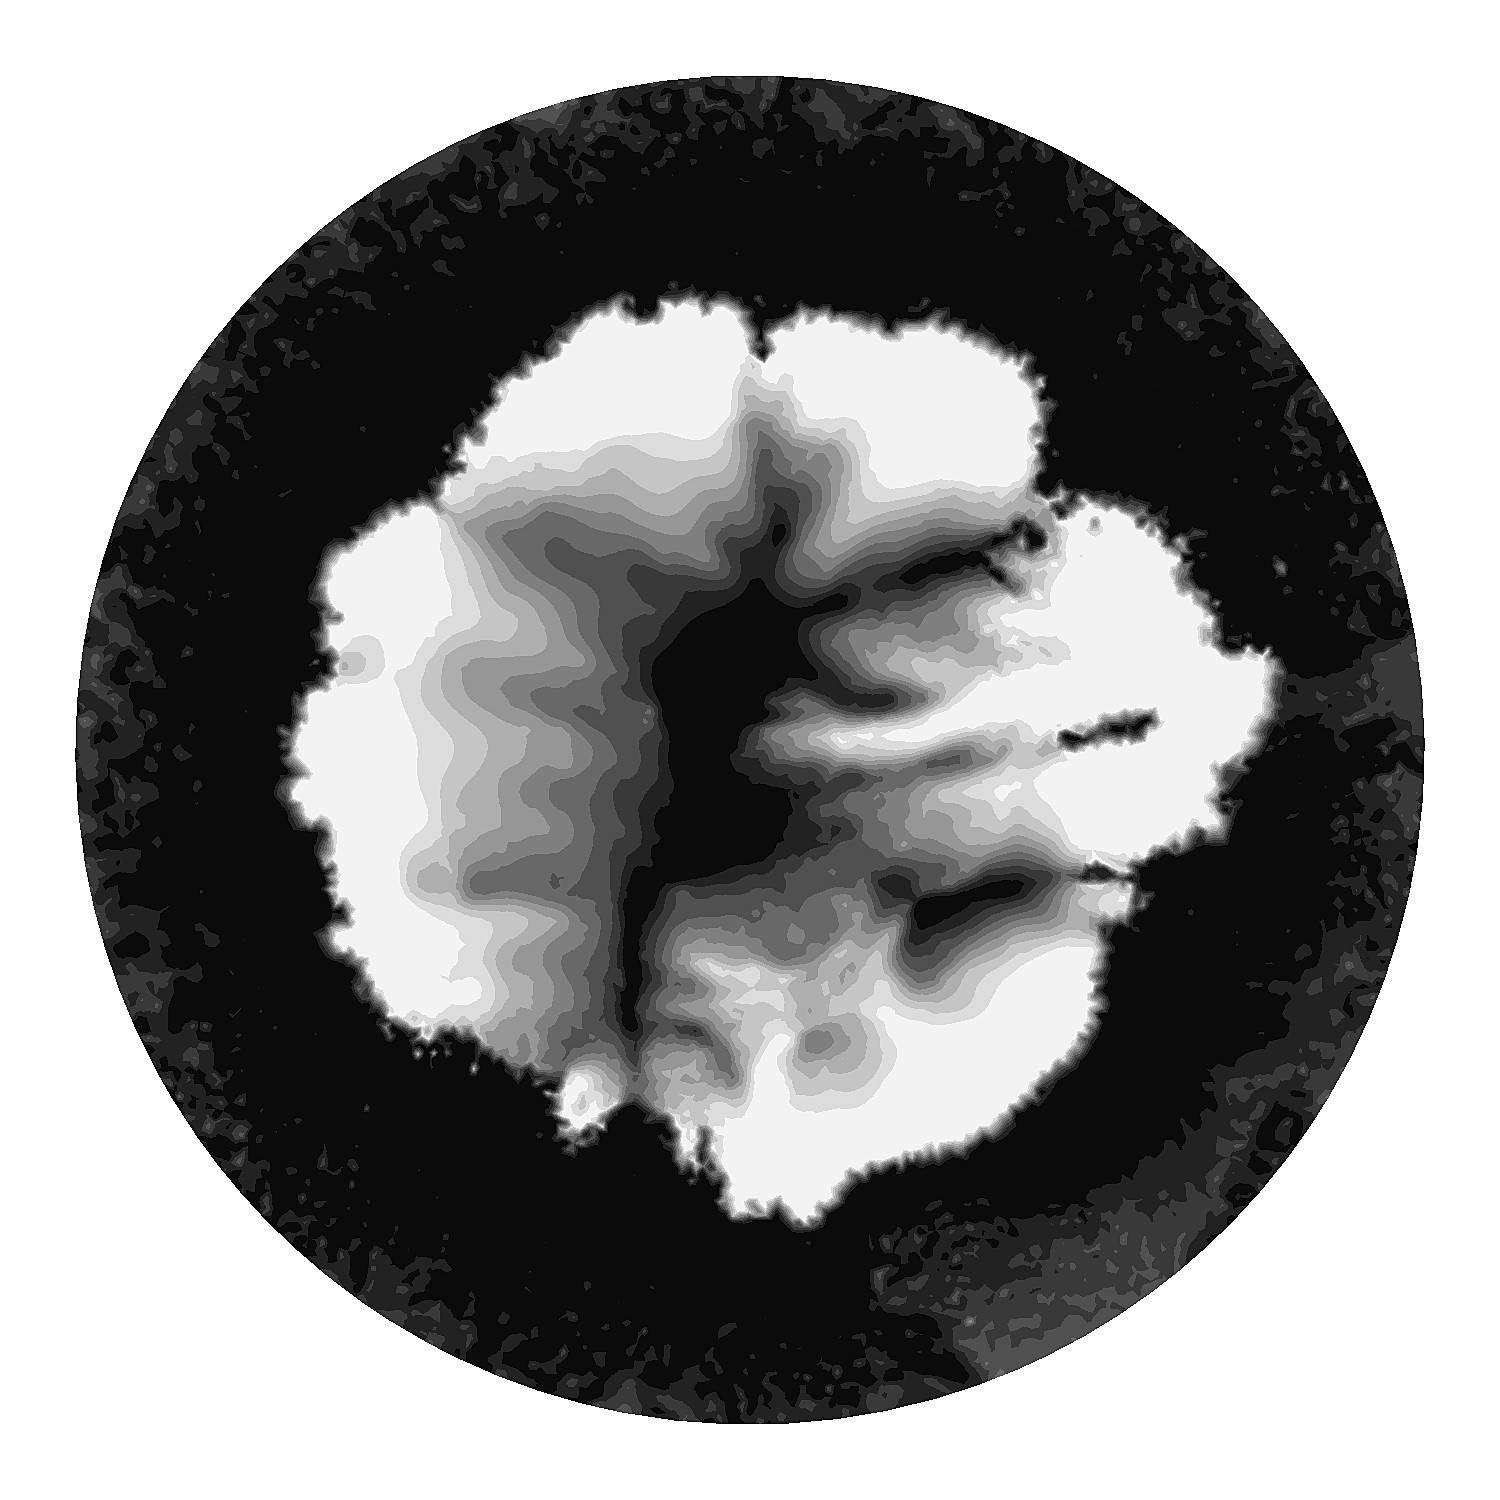
\includegraphics[width=1.0\textwidth]{images/EISMINT_II/U/beta_5000.jpg}
  \end{minipage}
  \quad
  \begin{minipage}[b]{0.30\linewidth}
    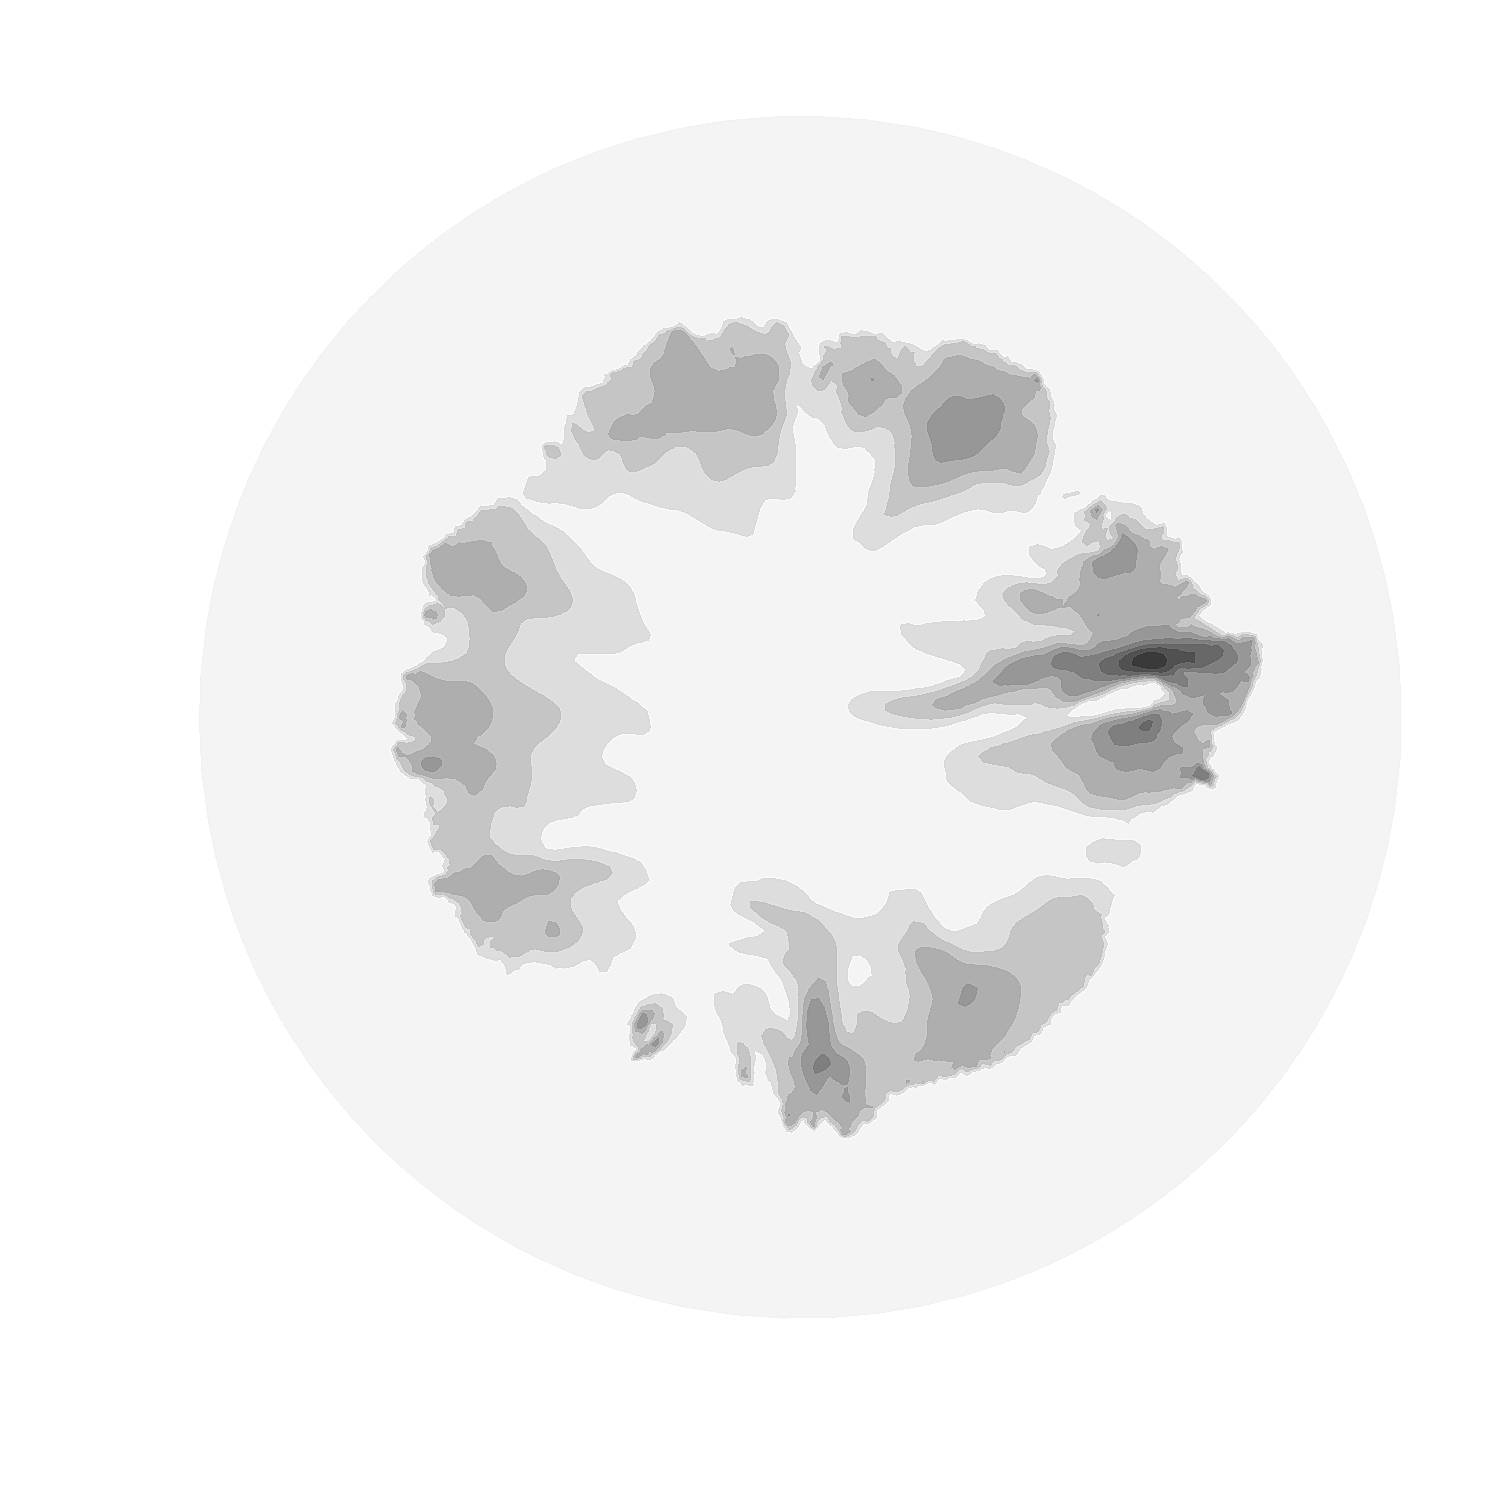
\includegraphics[width=1.0\textwidth]{images/EISMINT_II/U/U_mag_5000.jpg}
  \end{minipage}
  
  \begin{minipage}[b]{0.30\linewidth}
    \includegraphics[width=1.0\textwidth]{images/EISMINT_II/U/S_10000.jpg}
  \end{minipage}
  \quad
  \begin{minipage}[b]{0.30\linewidth}
    \includegraphics[width=1.0\textwidth]{images/EISMINT_II/U/beta_10000.jpg}
  \end{minipage}
  \quad
  \begin{minipage}[b]{0.30\linewidth}
    \includegraphics[width=1.0\textwidth]{images/EISMINT_II/U/U_mag_10000.jpg}
  \end{minipage}
  
  \begin{minipage}[b]{0.30\linewidth}
    \includegraphics[width=1.0\textwidth]{images/EISMINT_II/U/S_35000.jpg}
  \end{minipage}
  \quad
  \begin{minipage}[b]{0.30\linewidth}
    \includegraphics[width=1.0\textwidth]{images/EISMINT_II/U/beta_35000.jpg}
  \end{minipage}
  \quad
  \begin{minipage}[b]{0.30\linewidth}
    \includegraphics[width=1.0\textwidth]{images/EISMINT_II/U/U_mag_35000.jpg}
  \end{minipage}
  
  \begin{minipage}[b]{0.30\linewidth}
    \includegraphics[width=1.0\textwidth]{images/EISMINT_II/U/S_cb.jpg}
  \end{minipage}
  \quad
  \begin{minipage}[b]{0.30\linewidth}
    \includegraphics[width=1.0\textwidth]{images/EISMINT_II/U/beta_cb.jpg}
  \end{minipage}
  \quad
  \begin{minipage}[b]{0.30\linewidth}
    \includegraphics[width=1.0\textwidth]{images/EISMINT_II/U/U_mag_cb.jpg}
  \end{minipage}
  \caption[]{Surface height in meters (left), basal traction in (Pa a/m)$^{1/2}$ (middle), and surface speed in meters per annum (right) using the GLM-derived basal traction field using $\mathbf{u}_B$.  The time ranges from to to bottom : 500, 2000, 5000, 10000, and 35000 years.}
\end{figure}


\begin{figure}
  \centering
  
  \begin{minipage}[b]{0.30\linewidth}
    \includegraphics[width=1.0\textwidth]{images/EISMINT_II/Ubar/S_500.jpg}
  \end{minipage}
  \quad
  \begin{minipage}[b]{0.30\linewidth}
    \includegraphics[width=1.0\textwidth]{images/EISMINT_II/Ubar/beta_500.jpg}
  \end{minipage}
  \quad
  \begin{minipage}[b]{0.30\linewidth}
    \includegraphics[width=1.0\textwidth]{images/EISMINT_II/Ubar/U_mag_500.jpg}
  \end{minipage}
  
  \begin{minipage}[b]{0.30\linewidth}
    \includegraphics[width=1.0\textwidth]{images/EISMINT_II/Ubar/S_2000.jpg}
  \end{minipage}
  \quad
  \begin{minipage}[b]{0.30\linewidth}
    \includegraphics[width=1.0\textwidth]{images/EISMINT_II/Ubar/beta_2000.jpg}
  \end{minipage}
  \quad
  \begin{minipage}[b]{0.30\linewidth}
    \includegraphics[width=1.0\textwidth]{images/EISMINT_II/Ubar/U_mag_2000.jpg}
  \end{minipage}
  
  \begin{minipage}[b]{0.30\linewidth}
    \includegraphics[width=1.0\textwidth]{images/EISMINT_II/Ubar/S_5000.jpg}
  \end{minipage}
  \quad
  \begin{minipage}[b]{0.30\linewidth}
    \includegraphics[width=1.0\textwidth]{images/EISMINT_II/Ubar/beta_5000.jpg}
  \end{minipage}
  \quad
  \begin{minipage}[b]{0.30\linewidth}
    \includegraphics[width=1.0\textwidth]{images/EISMINT_II/Ubar/U_mag_5000.jpg}
  \end{minipage}
  
  \begin{minipage}[b]{0.30\linewidth}
    \includegraphics[width=1.0\textwidth]{images/EISMINT_II/Ubar/S_10000.jpg}
  \end{minipage}
  \quad
  \begin{minipage}[b]{0.30\linewidth}
    \includegraphics[width=1.0\textwidth]{images/EISMINT_II/Ubar/beta_10000.jpg}
  \end{minipage}
  \quad
  \begin{minipage}[b]{0.30\linewidth}
    \includegraphics[width=1.0\textwidth]{images/EISMINT_II/Ubar/U_mag_10000.jpg}
  \end{minipage}
  
  \begin{minipage}[b]{0.30\linewidth}
    \includegraphics[width=1.0\textwidth]{images/EISMINT_II/Ubar/S_35000.jpg}
  \end{minipage}
  \quad
  \begin{minipage}[b]{0.30\linewidth}
    \includegraphics[width=1.0\textwidth]{images/EISMINT_II/Ubar/beta_35000.jpg}
  \end{minipage}
  \quad
  \begin{minipage}[b]{0.30\linewidth}
    \includegraphics[width=1.0\textwidth]{images/EISMINT_II/Ubar/U_mag_35000.jpg}
  \end{minipage}
  
  \begin{minipage}[b]{0.30\linewidth}
    \includegraphics[width=1.0\textwidth]{images/EISMINT_II/Ubar/S_cb.jpg}
  \end{minipage}
  \quad
  \begin{minipage}[b]{0.30\linewidth}
    \includegraphics[width=1.0\textwidth]{images/EISMINT_II/Ubar/beta_cb.jpg}
  \end{minipage}
  \quad
  \begin{minipage}[b]{0.30\linewidth}
    \includegraphics[width=1.0\textwidth]{images/EISMINT_II/Ubar/U_mag_cb.jpg}
  \end{minipage}
  \caption[]{Surface height in meters (left), basal traction in (Pa a/m)$^{1/2}$ (middle), and surface speed in meters per annum (right) using the GLM-derived basal traction field using $\mathbf{\bar{u}}$.  The time ranges from to to bottom : 500, 2000, 5000, 10000, and 35000 years.}
\end{figure}

\begin{figure}
  \centering
  
  \begin{minipage}[b]{0.30\linewidth}
    \includegraphics[width=1.0\textwidth]{images/EISMINT_II/H/S_20000.jpg}
  \end{minipage}
  \quad
  \begin{minipage}[b]{0.30\linewidth}
    \includegraphics[width=1.0\textwidth]{images/EISMINT_II/H/beta_20000.jpg}
  \end{minipage}
  \quad
  \begin{minipage}[b]{0.30\linewidth}
    \includegraphics[width=1.0\textwidth]{images/EISMINT_II/H/U_mag_20000.jpg}
  \end{minipage}
  
  \begin{minipage}[b]{0.30\linewidth}
    \includegraphics[width=1.0\textwidth]{images/EISMINT_II/H/S_cb.jpg}
  \end{minipage}
  \quad
  \begin{minipage}[b]{0.30\linewidth}
    \includegraphics[width=1.0\textwidth]{images/EISMINT_II/H/beta_cb.jpg}
  \end{minipage}
  \quad
  \begin{minipage}[b]{0.30\linewidth}
    \includegraphics[width=1.0\textwidth]{images/EISMINT_II/H/U_mag_cb.jpg}
  \end{minipage}
  \caption[]{Surface height in meters (left), basal traction in (Pa a/m)$^{1/2}$ (middle), and surface speed in meters per annum (right) after 20000 years for the EISMINT II H experiment.  Basal traction is set to $\sqrt{1\mathrm{E}3}$ for areas where the temperature is below the pressure-melting point, and $\sqrt{1\mathrm{E}9}$ for areas above.}
\end{figure}
